%% Copyright 2012-2016 by abnTeX2 group at http://www.abntex.net.br/ 
%%
%% This work may be distributed and/or modified under the
%% conditions of the LaTeX Project Public License, either version 1.3
%% of this license or (at your option) any later version.
%% The latest version of this license is in
%%   http://www.latex-project.org/lppl.txt
%% and version 1.3 or later is part of all distributions of LaTeX
%% version 2005/12/01 or later.
%%
%% This work has the L PPL maintenance status `maintained'.
%% 
%% The Current Maintainer of this work is the abnTeX2 team, led
%% by Lauro César Araujo. Further information are available on 
%% http://www.abntex.net.br/
%%

% ------------------------------------------------------------------------
% ------------------------------------------------------------------------
% abnTeX2: Modelo de Trabalho Academico (tese de doutorado, dissertacao de
% mestrado e trabalhos monograficos em geral) em conformidade com 
% ABNT NBR 14724:2011: Informacao e documentacao - Trabalhos academicos -
% Apresentacao
% ------------------------------------------------------------------------
% ------------------------------------------------------------------------
% Personalização para o modelo Udesc 2020 7. ed. revisada e modificada
% MANUAL_2020_09_07_1599489825065_12510.pdf
% Autor: Felipe Joel Zimann (felipezimann@hotmail.com)
% Data: 02/12/2020 v1.0
% Data: 13/02/2021 v1.0.1 alterado tamanho numeração da página para 10pt
% ------------------------------------------------------------------------
% ------------------------------------------------------------------------

\documentclass[							% Descrição
	12pt,								% tamanho da fonte
	openright,							% capítulos começam em pág ímpar (insere página vazia caso preciso)
	oneside,							% para impressão em recto e verso (twoside). Oposto a (oneside)
	a4paper,							% tamanho do papel. 
	chapter=TITLE,						% títulos de capítulos convertidos em letras maiúsculas
	section=TITLE,						% títulos de seções convertidos em letras maiúsculas
	sumario=abnt-6027-2012,
	english,							% idioma adicional para hifenização
	brazil,								% o último idioma é o principal do documento
	fleqn,								% equações alinhadas a esquerda (UDESC/CCT)+
	]{abntex2}

% ----------------------------------------------------------
% Pacotes básicos 
% ----------------------------------------------------------
%\usepackage{fancyhdr}																																		% Pacote para deixar as figuras no cabeçalho
\usepackage{wrapfig} 																																		% Pacote para deixar as figuras ao lado do texto
\usepackage{acronym}																																		% Pacote para uso de acrônimos. Documentação: http://linorg.usp.br/CTAN/macros/latex/contrib/acronym/acronym.pdf
\usepackage{parcolumns} 																																	% Incluido para dividir os itemize em duas colunas
\usepackage{ragged2e}																																		% Incluido para usar o justify
\usepackage{amsmath}																																		% Pacote matemático
\usepackage{amssymb}																																		% Pacote matemático
\usepackage{amsfonts}																																		% Pacote matemático
%\usepackage{lmodern}																																		% Usa a fonte Latin Modern		
\usepackage{mathptmx} 																																		% Usa a fonte Times New Roman	 (UDESC/CCT)
\usepackage[T1]{fontenc}																																	% Selecao de codigos de fonte.
\usepackage[utf8]{inputenc}																																	% Codificacao do documento (conversão automática dos acentos)
\usepackage{lastpage}																																		% Usado pela Ficha catalográfica
\usepackage{indentfirst}																																	% Indenta o primeiro parágrafo de cada seção.
%\usepackage{pdfpages}																																		% Pacote para inserir PDFs
%\usepackage[dvipsnames,table]{xcolor}																														% Controle das cores
\usepackage{graphicx}																																		% Inclusão de gráficos
\usepackage{microtype} 																																		% para melhorias de justificação
\usepackage{lipsum}																																			% para geração de dummy text
\usepackage[brazilian,hyperpageref]{backref}																												% Paginas com as citações na bibl
\usepackage[alf,abnt-emphasize=bf,abnt-full-initials=yes]{abntex2cite}																						% Citações padrão ABNT
%\usepackage[num]{abntex2cite}																																% Citações padrão ABNT numérica
\usepackage{adjustbox}																																		% Pacote de ajuste de boxes
\usepackage{subcaption}																																		% Inclusão de Subfiguras e sublegendas		
\usepackage{enumitem}																																		% Personalização de listas
\usepackage{siunitx}																																		% Grandezas e unidades
\usepackage[section]{placeins}																																% Manter as figuras delimitadas na respectiva seção com a opção [section]
\usepackage{multirow}																																		% Multi colunas nas tabelas
\usepackage{array,tabularx} 																																% Pacotes de tabelas
\usepackage{booktabs}																																		% Pacote de tabela profissonal
\usepackage{rotating}																																		% Rotacionar figuras e tabelas
\usepackage{xfrac}																																			% Fazer frações n/d em linha
\usepackage{bm}																																				% Negrito em modo matemático
\usepackage{xstring}																																		% Manipulação de strings
\usepackage{pgfplots}																																		% Pacote de Gráficos
\usepackage{tikz}																																			% Pacote de Figuras
\usepackage[american, cuteinductors,smartlabels, fulldiode, siunitx, americanvoltages, oldvoltagedirection, smartlabels]{circuitikz}						% Pacote de circuitos elétricos
%\usepackage{chemformula}																																	% Pacote para fórmulas químicas
\usepackage{chngcntr}																																		% Pacte usado para deixar numeração de equações sequencial (UDESC/CCT)
\counterwithout{equation}{chapter}
% fonte: https://latex.org/forum/viewtopic.php?t=15392

% Comando para deixar numeração das equações contínua (1), (2), (3)... ao invés de organizar por capítulos (1.1)(1.2)... (2.1)(2.2)
%\renewcommand{\theequation}{\arabic{equation}}

%\numberwithin{equation}{section}


% Cabecalho cabeçalho somente com numeração de página 10pt
\makepagestyle{PagNumReduzida}
\makeevenhead{PagNumReduzida}{\ABNTEXfontereduzida\thepage}{}{}
\makeoddhead{PagNumReduzida}{}{}{\ABNTEXfontereduzida\thepage}
%fonte: https://github.com/abntex/abntex2/wiki/HowToCustomizarCabecalhoRodape
%fonte: Manual memoir seção 7.3 pg. 111 pdf http://linorg.usp.br/CTAN/macros/latex/contrib/memoir/memman.pdf 

% Personalização das opções das listas
\setlist[itemize]{leftmargin=\parindent}

% Citação online --- MODIFICAR ---
\newcommand{\citeshort}[1]{\citeauthoronline{#1}~(\citeyear{#1})}

\newcommand{\me}[1]{Elaborado pelo autor (#1).}

% Configuração do pgfplots
\pgfplotsset{compat=newest} %compat=1.14
\pgfplotsset{plot coordinates/math parser=false} 
\newlength\figureheight 
\newlength\figurewidth 

% Libraries do TiKz
\usetikzlibrary{quotes,angles,arrows}
\usetikzlibrary{through,calc,math}
\usetikzlibrary{graphs,backgrounds,fit}
\usetikzlibrary{shapes,positioning,patterns,shadows}
\usetikzlibrary{decorations.pathreplacing}
\usetikzlibrary{shapes.geometric}
\usetikzlibrary{arrows.meta}
\usetikzlibrary{external}

%\tikzexternalize[]
%\tikzexternalenable
%\tikzexternalize
%\tikzexternaldisable
%\tikzset{external/force remake}
%\tikzexternalize[shell escape=-enable-write18]

% Configurações do CircuiTiKz
\ctikzset{bipoles/thickness=1}
%\ctikzset{bipoles/length=1.2cm}
\ctikzset{monopoles/ground/width/.initial=.2}
\ctikzset{bipoles/resistor/height=0.25}
\ctikzset{bipoles/resistor/width=0.6}
\ctikzset{bipoles/capacitor/height=0.5}
\ctikzset{bipoles/capacitor/width=0.15}
\ctikzset{bipoles/generic/height=0.25}
\ctikzset{bipoles/generic/width=0.6}
%\ctikzset{bipoles/capacitor polar/length=0.5}
%\ctikzset{bipoles/diode/height=.375}
%\ctikzset{bipoles/diode/width=.3}
%\ctikzset{tripoles/thyristor/height=.8}
%\ctikzset{tripoles/thyristor/width=1}
\ctikzset{bipoles/vsourcesin/height=.5}
\ctikzset{bipoles/vsourcesin/width=.5}
\ctikzset{bipoles/cvsourceam/height=.6}
\ctikzset{bipoles/cvsourceam/width=.6}
%\ctikzset{tripoles/european controlled voltage source/width=.4}

\tikzstyle{every node}=[font=\footnotesize]
\tikzstyle{every path}=[line width=0.25pt,line cap=round,line join=round]
%\tikzstyle{every path}=[line cap=round,line join=round]


% Definição de cores MATLAB
\definecolor{matlab_blue}{rgb}	{         0,    0.4470,    0.7410}
\definecolor{matlab_orange}{rgb}{    0.8500,    0.3250,    0.0980}
\definecolor{matlab_yellow}{rgb}{    0.9290,    0.6940,    0.1250}
\definecolor{matlab_violet}{rgb}{    0.4940,    0.1840,    0.5560}
\definecolor{matlab_green}{rgb}	{	 0.4660,    0.6740,    0.1880}
\definecolor{matlab_lblue}{rgb}	{    0.3010,    0.7450,    0.9330}
\definecolor{matlab_red}{rgb}	{    0.6350,    0.0780,    0.1840}

% Personalização das legendas
\usepackage[format = plain, %hang
			justification = centering,
			labelsep = endash,
			singlelinecheck = false,
			skip = 6pt,
			listformat = simple]{caption}	

% Personalização das unidades
\sisetup{output-decimal-marker = {,}}
\sisetup{exponent-product = \cdot, output-product = \cdot}
\sisetup{tight-spacing=true}
\sisetup{group-digits = false}

% Personalizações de tipo de colunas de tabelas
\newcolumntype{L}[1]{>{\raggedright\let\newline\\\arraybackslash\hspace{0pt}}m{#1}}
\newcolumntype{C}[1]{>{\centering\let\newline\\\arraybackslash\hspace{0pt}}m{#1}}
\newcolumntype{R}[1]{>{\raggedleft\let\newline\\\arraybackslash\hspace{0pt}}m{#1}}

% Personalizações de cores da UDESC
\definecolor{CapaAmareloUDESC}{RGB}{243,186,83}		% Especializacao
\definecolor{CapaVerdeUDESC}{RGB}{0,112,52}			% Mestrado
\definecolor{CapaVermelhoUDESC}{RGB}{171,35,21}		% Doutorado
\definecolor{CapaAzulUDESC}{RGB}{38,54,118} 		% Pós-Doutorado

% CONFIGURAÇÕES DE PACOTES
% Configurações do pacote backref
% Usado sem a opção hyperpageref de backref
\renewcommand{\backrefpagesname}{Citado na(s) página(s):~}
% Texto padrão antes do número das páginas
\renewcommand{\backref}{}
% Define os textos da citação
\renewcommand*{\backrefalt}[4]{
	\ifcase #1 %
	Nenhuma citação no texto.%
	\or
	Citado na página #2.%
	\else
	Citado #1 vezes nas páginas #2.%
	\fi}%

% alterando o aspecto da cor azul
%\definecolor{blue}{RGB}{41,5,195}

% informações do PDF
\makeatletter
\hypersetup{
	%pagebackref=true,
	pdftitle={\@title}, 
	pdfauthor={\@author},
	pdfsubject={\imprimirpreambulo},
	pdfcreator={LaTeX with abnTeX2},
	pdfkeywords={abnt}{latex}{abntex}{abntex2}{trabalho academico}, 
	colorlinks=true,       		% false: boxed links; true: colored links
	linkcolor=black,          	% color of internal links
	citecolor=black,        	% color of links to bibliography
	filecolor=black,      		% color of file links
	urlcolor=black,
	bookmarksdepth=4
}
\makeatother


\makeatletter
\newcommand{\includetikz}[1]{%
	\tikzsetnextfilename{#1}%
	\input{#1.tex}%
}
\makeatother

% ---
% Possibilita criação de Quadros e Lista de quadros.
% Ver https://github.com/abntex/abntex2/issues/176
%
\newcommand{\quadroname}{Quadro}
\newcommand{\listofquadrosname}{Lista de quadros}

\newfloat[chapter]{quadro}{loq}{\quadroname}
\newlistof{listofquadros}{loq}{\listofquadrosname}
\newlistentry{quadro}{loq}{0}

% configurações para atender às regras da ABNT
\setfloatadjustment{quadro}{\centering}
\counterwithout{quadro}{chapter}
\renewcommand{\cftquadroname}{\quadroname\space} 
\renewcommand*{\cftquadroaftersnum}{\hfill--\hfill}

\setfloatlocations{quadro}{hbtp} % Ver https://github.com/abntex/abntex2/issues/176
% ---


% Espaçamento depois do título
\setlength{\afterchapskip}{0.7\baselineskip}
% O tamanho do parágrafo é dado por:
\setlength{\parindent}{1.25cm}
% Controle do espaçamento entre um parágrafo e outro:
\setlength{\parskip}{0.0cm}  % tente também \onelineskip
%\SingleSpacing % Espaçamento simples 
\OnehalfSpacing % Espaçamento 1,5 (UDESC/CCT)
%\DoubleSpacing	% Espaçamento duplo

% ---
% Margens - NBR 14724/2011 - 5.1 Formato
% ---
\setlrmarginsandblock{3cm}{2cm}{*}
\setulmarginsandblock{3cm}{2cm}{*}
\checkandfixthelayout[fixed]
% ---


% To use externalize consider
%https://tex.stackexchange.com/questions/182783/tikzexternalize-not-compatible-with-miktex-2-9-abntex2-package
%Lauro Cesar digged into the problem until he came with a solution for me to test. And it Works!
%
%According to this link:
%
%The package calc changed the commands \setcounter and friends to be fragile. So you have to make them robust. The example below uses etoolbox with \robustify:
%
\usepackage{etoolbox}
\robustify\setcounter
\robustify\addtocounter
\robustify\setlength
\robustify\addtolength


%% How to silence memoir class warning against the use of caption package?
%% https://tex.stackexchange.com/questions/391993/how-to-silence-memoir-class-warning-against-the-use-of-caption-package
%\usepackage{silence}
%\WarningFilter*{memoir}{You are using the caption package with the memoir class}
%\WarningFilter*{Class memoir Warning}{You are using the caption package with the memoir class}

% --------------------------------------------------------
% INICIO DAS CUSTOMIZACOES PARA A UDESC
% --------------------------------------------------------

% --------------------------------------------------------
% Fontes padroes de part, chapter, section, subsection e subsubsection
% --------------------------------------------------------
% --- Chapter ---
\renewcommand{\ABNTEXchapterfont}{\fontseries{b}} %\bfseries
\renewcommand{\ABNTEXchapterfontsize}{\normalsize}
% --- Part ---
\renewcommand{\ABNTEXpartfont}{\ABNTEXchapterfont}
\renewcommand{\ABNTEXpartfontsize}{\LARGE}
% --- Section ---
\renewcommand{\ABNTEXsectionfont}{\normalfont}
\renewcommand{\ABNTEXsectionfontsize}{\normalsize}
% --- SubSection ---
\renewcommand{\ABNTEXsubsectionfont}{\fontseries{b}} %\bfseries
\renewcommand{\ABNTEXsubsectionfontsize}{\normalsize}
% --- SubSubSection ---
\renewcommand{\ABNTEXsubsubsectionfont}{\itshape}
\renewcommand{\ABNTEXsubsubsectionfontsize}{\normalsize}

\renewcommand{\ABNTEXsubsubsubsectionfont}{\normalfont}
\renewcommand{\ABNTEXsubsubsubsectionfontsize}{\normalsize}
% ---

% --------------------------------------------------------
% Fontes das entradas do sumario
% --------------------------------------------------------

\renewcommand{\cftpartfont}{\ABNTEXpartfont\selectfont}
\renewcommand{\cftpartpagefont}{\normalsize\selectfont}

\renewcommand{\cftchapterfont}{\ABNTEXchapterfont\selectfont}
\renewcommand{\cftchapterpagefont}{\normalsize\selectfont}

\renewcommand{\cftsectionfont}{\ABNTEXsectionfont\selectfont}
\renewcommand{\cftsectionpagefont}{\normalsize\selectfont}

\renewcommand{\cftsubsectionfont}{\ABNTEXsubsectionfont\selectfont}
\renewcommand{\cftsubsectionpagefont}{\normalsize\selectfont}

\renewcommand{\cftsubsubsectionfont}{\normalfont\itshape\selectfont}
\renewcommand{\cftsubsubsectionpagefont}{\normalsize\selectfont}

\renewcommand{\cftparagraphfont}{\normalfont\selectfont}
\renewcommand{\cftparagraphpagefont}{\normalsize\selectfont}

% --------------------------------------------------------
% Usando os pacotes hyperref, uppercase... 
% Para deixar a section do toc uppercase precisa de:
% --------------------------------------------------------
\usepackage{textcase}

\makeatletter

\let\oldcontentsline\contentsline
\def\contentsline#1#2{%
	\expandafter\ifx\csname l@#1\endcsname\l@section
	\expandafter\@firstoftwo
	\else
	\expandafter\@secondoftwo
	\fi
	{%
		\oldcontentsline{#1}{\MakeTextUppercase{#2}}%
	}{%
		\oldcontentsline{#1}{#2}%
	}%
}
\makeatother

% --------------------------------------------------------
% Renomenando as entradas de APÊNDICES E ANEXOS
% --------------------------------------------------------

\renewcommand{\apendicesname}{AP\^ENDICES}
\renewcommand{\anexosname}{ANEXOS}
\newcommand{\refanexo}[1]{\hyperref[#1]{Anexo~\ref{#1}}} 						%Esse comando é para arrumar a chamada via ponteiro (que estava chamando anexos como apêndices) [usar \refanexo{} ao invés de \autoref{}]


% Manipulação de Strings
%\RequirePackage{xstring}

% Comando para inverter sobrenome e nome
\newcommand{\invertname}[1]{%
	\StrBehind{#1}{{}}, \StrBefore{#1}{{}}%
}%


% --------------------------------------------------------
% Alterando os estilos de Caption e Fonte
% --------------------------------------------------------
\makeatletter
% Define o comando \fonte que respeita as configurações de caption do memoir ou do caption
\renewcommand{\fonte}[2][\fontename]{%
	\M@gettitle{#2}%
	\memlegendinfo{#2}%
	\par
	\begingroup
	\@parboxrestore
	\if@minipage
	\@setminipage
	\fi
	\ABNTEXfontereduzida
	\configureseparator
	\captiondelim{\ABNTEXcaptionfontedelim}
	\@makecaption{#1}{\ignorespaces #2}\par
	\endgroup}


\captionstyle[\raggedright]{\raggedright}

\makeatother

\setlength{\cftbeforechapterskip}{0pt plus 0pt}
\renewcommand*{\insertchapterspace}{}

\newlength{\mylen}	% New length to use with spacing
\setlength{\mylen}{1pt}

\setlength{\cftbeforechapterskip}{\mylen}
\setlength{\cftbeforesectionskip}{\mylen}
\setlength{\cftbeforesubsectionskip}{\mylen}
\setlength{\cftbeforesubsubsectionskip}{\mylen}
\setlength{\cftbeforesubsubsubsectionskip}{\mylen}


% ---
% Ajuste das listas de abreviaturas e siglas ; e símbolos [Personalizada para UDESC com espaçamento 1,5]
% ---

% ---
% Redefinição da Lista de abreviaturas e siglas [Personalizada para UDESC com espaçamento 1,5]
\renewenvironment{siglas}{%
	\pretextualchapter{\listadesiglasname}
}
% ---
 

% ---
% Redefinição da Lista de símbolos [Personalizada para UDESC com espaçamento 1,5]
\renewenvironment{simbolos}{%
	\pretextualchapter{\listadesimbolosname}
	\begin{symbols}
		\setlength{\itemsep}{0pt}	% Ajuste para Espaçamento 1,5 (UDESC/CCT)
	}{%
	\end{symbols}
	\cleardoublepage
}
% ---




% ---
% FIM DAS CUSTOMIZACOES PARA A  Universidade do Estado de Santa Catarina - UDESC/CCT
% ---					% Incliu pacotes básicos 

% -----------------------------------------------------------------
% Você pode adicionar seus pacotes a partir desta linha;
% -----------------------------------------------------------------

%\usepackage[showframe,pass]{geometry}
%\usepackage[11,12]{pagesel}

% -----------------------------------------------------------------
% Informações de dados para CAPA e FOLHA DE ROSTO
% -----------------------------------------------------------------

\titulo{Um Jogo como Tecnologia Educacional para \\ Prevenção da Violência Sexual Infantil}%

\autor{Alexandre {}Mendonça Fava}%
\orientador[Orientadora:]{Carla {}Diacui Medeiros Berkenbrock}%
\coorientador{Adilson {}Vahldick}%

% ATENÇÃO: O símbolo {} indica o sobrenome para a ficha catalográfica.
% Exemplo: Sherlock Holmes {}da Silva para sobrenomes compostos;
% Exemplo: Arnold Alois {}Schwarzenegger para sobrenome simples.

\instituicao{Universidade do Estado de Santa Catarina, Centro de Ciências Tecnológicas, Programa de Pós--Graduação em Computação Aplicada}%

%\tipotrabalho{Tese (Doutorado)}
\tipotrabalho{Dissertação (Mestrado)}

%\preambulo{Tese apresentada ao Programa de Pós--Graduação em Computação Aplicada do Centro de Ciências Tecnológicas da Universidade do Estado de Santa Catarina, como requisito parcial para a obtenção do grau de Doutor em Computação Aplicada.}

\preambulo{Dissertação apresentada ao Programa de Pós--Graduação em Computação Aplicada do Centro de Ciências Tecnológicas da Universidade do Estado de Santa Catarina, para a obtenção do grau de Mestre em Computação Aplicada.}

\local{Joinville}%

\data{\the\year}%
% ---

% compila o indice
\makeindex

% -----------------------------------------------------------------
% Início do documento
% -----------------------------------------------------------------
\begin{document}

\selectlanguage{brazil}
\frenchspacing  % Retira espaço extra obsoleto entre as frases.

% -----------------------------------------------------------------
% ELEMENTOS PRÉ-TEXTUAIS
% -----------------------------------------------------------------
\pretextual

% Você pode comentar os elementos que não deseja em seu trabalho;

% A capa pode ser escolhida dentro do arquivo Capa.tex (TCC, Master, Doc, ...)
% Caso não utilize a Ficha Catalográfica entre na folha de rosto e retire o * de dentro do arquivo FolhadeRosto
% --------------------------------------------------------
% Capa Padrão
% --------------------------------------------------------

\renewcommand{\imprimircapa}{%
	\begin{capa}%
		\center

		{\fontseries{b}\selectfont\MakeTextUppercase{UNIVERSIDADE DO ESTADO DE SANTA CATARINA -- UDESC}}
		
		{\fontseries{b}\selectfont\MakeTextUppercase{CENTRO DE CIÊNCIA TECNOLÓGICAS -- CCT  }}
		
		{\fontseries{b}\selectfont\MakeTextUppercase{PROGRAMA DE PÓS-GRADUAÇÃO EM COMPUTAÇÃO APLICADA -- PPGCAP  }}
		
		\vfill
		
		{\fontseries{b}\selectfont\MakeTextUppercase{\normalsize\imprimirautor}}
		
		\vfill
		\begin{center}
			{\fontseries{b}\selectfont\MakeTextUppercase{\imprimirtitulo}}
		\end{center}
		\vfill
		
		\vfill
		
		{\fontseries{b}\selectfont\MakeTextUppercase{\imprimirlocal}}
		\par
		{\fontseries{b}\selectfont \imprimirdata}
		\vspace*{1cm}
	\end{capa}
}

\imprimircapa				% Capa padrão					% Elemento Obrigatório
% ---
% Folha de rosto
% ---








% --------------------------------------------------------
% folha de rosto 
% --------------------------------------------------------

\makeatletter

\renewcommand{\folhaderostocontent}{
	\begin{center}
		
		{\fontseries{b}\selectfont\MakeTextUppercase{\imprimirautor}}
		
		\vfill
		
		\begin{center}
			{\fontseries{b}\selectfont\MakeTextUppercase{\imprimirtitulo}}
		\end{center}
	
		\vspace*{1.5cm}

		\abntex@ifnotempty{\imprimirpreambulo}{%
			\hspace{.45\textwidth}
			{\begin{minipage}{.5\textwidth}
					\SingleSpacing
					\imprimirpreambulo\par
					\vspace*{4pt}
					{\imprimirorientadorRotulo~\imprimirorientador\par}
					\abntex@ifnotempty{\imprimircoorientador}{%
						{\imprimircoorientadorRotulo~\imprimircoorientador}%
					}%
			\end{minipage}}%
		}%
	
		
		\vfill
		
	{\fontseries{b}\selectfont\MakeTextUppercase{\imprimirlocal}}
	\par
	{\fontseries{b}\selectfont \imprimirdata}
	\vspace*{1cm}
	\end{center}
}


% (o * indica que haverá a ficha bibliográfica)
% ---
\imprimirfolhaderosto*
% ---


			% Elemento Obrigatório

% ---
% Inserir a ficha bibliografica
% ---

% Isto é um exemplo de Ficha Catalográfica, ou ``Dados internacionais de
% catalogação-na-publicação''. Você pode utilizar este modelo como referência. 
% Porém, provavelmente a biblioteca da sua universidade lhe fornecerá um PDF
% com a ficha catalográfica definitiva após a defesa do trabalho. Quando estiver
% com o documento, salve-o como PDF no diretório do seu projeto e substitua todo
% o conteúdo de implementação deste arquivo pelo comando abaixo:



% \begin{fichacatalografica}
%     \includepdf{fig_ficha_catalografica.pdf}
% \end{fichacatalografica}


%	\setlength{\parindent}{0cm}
%	\setlength{\parskip}{0pt}
\begin{fichacatalografica}
	%\sffamily
	%\rmfamily
	\ttfamily \hbadness=10000
	\vspace*{\fill}					% Posição vertical
	\begin{center}					% Minipage Centralizado
	Para gerar a ficha catalográfica de teses e \\ 
	dissertações acessar o link:  \\
	https://www.udesc.br/bu/manuais/ficha
	
	\vspace*{8pt}
	
%	\begin{minipage}[c]{8cm}
%	\centering \sffamily
%	 Ficha catalográfica elaborada pelo(a) autor(a), com auxílio do programa de geração automática da Biblioteca Setorial do CCT/UDESC
%	\end{minipage}
	\fbox{\begin{minipage}[c]{12.5cm}		% Largura
	\flushright
	{\begin{minipage}[c]{10.5cm}		% Largura
	\vspace{1.25cm}
	%\footnotesize
	\setlength{\parindent}{1.5em}
	\noindent \invertname{\imprimirautor} \par
	\imprimirtitulo{ }/{ }\imprimirautor. -- \imprimirlocal, \imprimirdata .\par
	\pageref{LastPage} p. : il. ; 30 cm.\par
	\vspace{1.5em}
	\imprimirorientadorRotulo~\imprimirorientador.\par
	\imprimircoorientadorRotulo~\imprimircoorientador.\par
	\imprimirtipotrabalho~--~\imprimirinstituicao, \imprimirlocal, \imprimirdata.\par
	\vspace{1.5em}
		1. Tecnologia Educacional.
		2. Prevenção.
		3. Violência Sexual Infantil.
		I. \invertname{\imprimirorientador}.
		II. \invertname{\imprimircoorientador}.
		III. \imprimirinstituicao.
		IV. Título. %
	\vspace{1.25cm}	%		
	\end{minipage}%
	}% 
	\end{minipage}}%
	
	\vspace*{0.5cm}
	
	\end{center}
\end{fichacatalografica}


%\begin{fichacatalografica}
%	\sffamily
%	\vspace*{\fill}					% Posição vertical
%	\begin{center}					% Minipage Centralizado
%	\fbox{\begin{minipage}[c][8cm]{13.5cm}		% Largura
%	\small
%	\imprimirautor
%	%Sobrenome, Nome do autor
%	
%	\hspace{0.5cm} \imprimirtitulo  / \imprimirautor. --
%	\imprimirlocal, \imprimirdata-
%	
%	\hspace{0.5cm} \pageref{LastPage} p. : il. (algumas color.) ; 30 cm.\\
%	
%	\hspace{0.5cm} \imprimirorientadorRotulo~\imprimirorientador\\
%	
%	\hspace{0.5cm}
%	\parbox[t]{\textwidth}{\imprimirtipotrabalho~--~\imprimirinstituicao,
%	\imprimirdata.}\\
%	
%	\hspace{0.5cm}
%		1. Palavra-chave1.
%		2. Palavra-chave2.
%		3. Palavra-chave3.
% 		4. Palavra-chave4.
%		5. Palavra-chave5.
%		I. Orientador.
%		II. Universidade xxx.
%		III. Faculdade de xxx.
%		IV. Título 			
%	\end{minipage}}
%	\end{center}
%\end{fichacatalografica}
% ---

	% Elemento Obrigatório (Verso da Folha)
%
% ---
% Inserir errata
% ---
\begin{errata}
Elemento opcional. 

Exemplo:

\vspace{\onelineskip}

SOBRENOME, Prenome do Autor. Título de obra: subtítulo (se houver). Ano de depósito. Tipo do trabalho (grau e curso) - Vinculação acadêmica, local de apresentação/defesa, data.

\begin{table}[htb]
\center
\begin{tabular}{|p{2.4cm}|p{2cm}|p{3cm}|p{3cm}|}
  \hline
   \textbf{Folha} & \textbf{Linha}  & \textbf{Onde se lê}  & \textbf{Leia-se}  \\
    \hline
    1 & 10 & auto-conclavo & autoconclavo\\
   \hline
\end{tabular}
\end{table}

\end{errata}
% ---				% Elemento Opcional

% ---
% Inserir folha de aprovação
% ---

% Isto é um exemplo de Folha de aprovação, elemento obrigatório da NBR
% 14724/2011 (seção 4.2.1.3). Você pode utilizar este modelo até a aprovação
% do trabalho. Após isso, substitua todo o conteúdo deste arquivo por uma
% imagem da página assinada pela banca com o comando abaixo:
%
% \includepdf{folhadeaprovacao_final.pdf}
%
\begin{folhadeaprovacao}

	\begin{center}
		{\fontseries{b}\selectfont\MakeTextUppercase{\normalsize\imprimirautor}}
	\end{center}
    \vfill
    
	\vfill
	\begin{center}
		{\fontseries{b}\selectfont\MakeTextUppercase{\imprimirtitulo}}
	\end{center}
	\vfill

\abntex@ifnotempty{\imprimirpreambulo}{%
	\hspace{.45\textwidth}
	{\begin{minipage}{.5\textwidth}
			\SingleSpacing
			\imprimirpreambulo\par
			\vspace*{4pt}
%			{\imprimirorientadorRotulo~\imprimirorientador\par}
%			\abntex@ifnotempty{\imprimircoorientador}{%
%				{\imprimircoorientadorRotulo~\imprimircoorientador}%
%			}%
	\end{minipage}}%
}%


\vfill
        
	 \begin{center}
	 	
    	{\fontseries{b}\selectfont BANCA EXAMINADORA}
    	\vspace*{0.25cm}
    
		\assinatura{Dra. Carla Diacui Medeiros Berkenbrock} \par
		\vspace{0.15cm}
		Universidade do Estado de Santa Catarina

		%\vspace*{1.25cm}
		\assinatura{Dr. Adilson Vahldick} \par
		\vspace{0.15cm}
		Universidade do Estado de Santa Catarina

	 \end{center}
	
    {Membros:} 
    
	\begin{center}
		\vspace*{-1.25cm}
		\assinatura{Dr. Luciano Heitor Gallegos Marin} \par
		\vspace{0.15cm}
		Universidade de Fortaleza
		
		%\vspace*{1.25cm}
		\assinatura{Dra. Vera Márcia Marques Santos} \par
		\vspace{0.15cm}
		Universidade do Estado de Santa Catarina

	
	\end{center}
    
    \vspace*{\fill}  
    \begin{center}
    {\imprimirlocal, 16 de dezembro de \imprimirdata} %Essa deve ser a data de defesa
	\end{center}
    \vspace*{0.25cm}  
\end{folhadeaprovacao}
% ---




%\textbf{	{Orientador: \vspace{-16pt} }
%	\assinatura{\textbf{Prof. \imprimirorientador , Dr.} \\ Univ. XXX} 
%	{Coorientador: \vspace{-16pt}}   
%	\assinatura{\textbf{Prof. \imprimircoorientador , Dr.} \\ Univ. XXX}
%	
%	{Membros: \vspace{-16pt} } 
%	
%	% --- Exemplo de assinaturas em sequência ---       
%	\setlength{\ABNTEXsignwidth}{8.5cm}
%	
%	\assinatura{\textbf{Prof. Professor, Dr.} \\ Univ. XXX}
%	\assinatura{\textbf{Prof. Professor, Dr.} \\ Univ. XXX}
%	\assinatura{\textbf{Prof. Professor, Dr.} \\ Univ. XXX}
%	
%	% --- Exemplo de assinaturas lado a lado ---
%	\setlength{\ABNTEXsignwidth}{7.5cm}
	%
	%    \noindent\hfill\assinatura*{\textbf{Prof. Professor, Dr.} \\ Univ. XXX}%
	%    \hfill%
	%    \assinatura*{\textbf{Prof. Professor, Dr.} \\ Univ. XXX}%
	%    \hfill
	%    
	%    \noindent\hfill\assinatura*{\textbf{Prof. Professor, Dr.} \\ Univ. XXX}%
	%    \hfill%
	%    \assinatura*{\textbf{Prof. Professor, Dr.} \\ Univ. XXX}%
	%    \hfill}		% Elemento Obrigatório
% ---
% Dedicatória
% ---
\begin{dedicatoria}
   \vspace*{\fill}
%   \begin{flushright}
%   \noindent
%	Este trabalho é dedicado às crianças adultas que,\\
%	quando pequenas, sonharam em se tornar cientistas. 
%   \end{flushright}

{%
	\noindent\hspace{.5\textwidth}
	{\begin{minipage}{.5\textwidth}
			\begin{flushleft}
				Dedico este trabalho a todos os gigantes. %Se eu vi mais longe, foi por estar sobre ombros de gigantes.
				%Dedico este trabalho a todos aqueles que esqueci de agradecer nos meus agradecimentos.
				%A todos os amantes de jogos que acreditam que, além de gerar horas e mais horas de entretenimento e diversão, estes também podem ser utilizados para ensinar e aprender de forma mais descontraída e, quem sabe, de forma mais eficaz. %https://www.udesc.br/arquivos/cct/id_cpmenu/1024/diego_buchinger__1__15167055468902_1024.pdf
			\end{flushleft}
	\end{minipage}}%
\vspace*{3cm}
}%

\end{dedicatoria}
% ---
			% Elemento Opcional
% ---
% Agradecimentos
% ---
\begin{agradecimentos}

O presente trabalho foi realizado com apoio da Coordenação de Aperfeiçoamento de Pessoal de Nível Superior - Brasil (CAPES) - Código de Financiamento 001.

\end{agradecimentos}
% ---		% Elemento Opcional
%% ---
% Epígrafe
% ---
\begin{epigrafe}
    \vspace*{\fill}
%	\begin{flushright}
%		\textit{``Eu não falhei, encontrei 10 mil soluções que não davam certo.'' (EDISON, [19--])}
%	\end{flushright}
{%
	\noindent\hspace{.5\textwidth}
	{\begin{minipage}{.5\textwidth}
		\begin{flushright}
			``O que se faz agora com as crianças é o que elas farão depois com a sociedade.'' %(KARL MANNHEIM, [--]) Não encontrei fonte confiável de onde essa frase foi citada
		\end{flushright}
	\end{minipage}}%
	\vspace*{3cm}
}%
\end{epigrafe}
% ---				% Elemento Opcional (necessita de fonte bibliográfica)
% ---
% RESUMOS
% ---

% resumo em português
\setlength{\absparsep}{8pt} % ajusta o espaçamento dos parágrafos do resumo [aqui estava 18 antes]
\begin{resumo}
   %Elemento obrigatório que contém a apresentação concisa dos pontos relevantes do trabalho, fornecendo uma visão rápida e clara do conteúdo e das conclusões do mesmo. A apresentação e a redação do resumo devem seguir os requisitos estipulados pela NBR 6028 (ABNT, 2003). Deve descrever de forma clara e sintética a natureza do trabalho, o objetivo, o método, os resultados e as conclusões, visando fornecer elementos para o leitor decidir sobre a consulta do trabalho no todo.
  A violência sexual infantil é um grave problema de saúde pública. Tal problema traz prejuízos tanto às vítimas, quanto à sociedade. Em resposta a esse fenômeno, inúmeras medidas surgiram ao redor do globo, voltadas à proteção dos direitos das crianças e dos adolescentes. Dentre as medidas, estratégias educativas baseadas em jogos se destacam, demonstrando-se como boas aliadas no ensino preventivo e no combate à violência sexual infantil. 
  A presente pesquisa acadêmica realizou o desenvolvimento de um jogo sério focado na ensino-aprendizagem da prevenção da violência sexual. Os conteúdos pedagógicos abordados no jogo são projetados para crianças entre 5 (cinco) e 8 (oito) anos de idade. O principal objetivo do jogo consiste na ideia de educar e conscientizar seus jogadores a identificar e relatar eventos praticados (ou tentados) de violência sexual infantil. Buscando atender o rigor do processo científico, a presente pesquisa realiza um ensaio, de modo a avaliar se o jogo em si é capaz de cumprir com seus preceitos pré-estabelecidos. 
  O processo avaliativo do jogo desenvolvido foi realizado com uma amostra de 33 (trinta e três) crianças da Escola Municipal Pauline Parucker. Todos os experimentos envolvendo a amostra de crianças foram conduzidos na própria escola. % (idade média de 8 anos). 
  A amostra de crianças foi segmentada em dois grupos; grupo controle (n = 18) e grupo experimental (n = 15). O grupo experimental foi exposto ao jogo na etapa de teste da presente pesquisa. Ambos os grupos tiveram seus conhecimentos sobre prevenção ao abuso mensurados pelo instrumento avaliativo \ac{CKAQ}. Os conhecimentos dos grupos foram mensurados na etapa de pré-teste e na etapa de pós-teste da corrente pesquisa, de modo a identificar seus níveis de instrução sobre prevenção ao abuso. 
  A análise dos dados não apresentou discrepância sobre os níveis de instrução entre os grupos estudados. Não foi possível identificar estatisticamente nível de influência do jogo no que diz respeito ao ensino de seus preceitos pré-estabelecidos (p = 0,27697). Em síntese, ambos os grupos estudados apresentaram graus de conhecimento semelhantes na etapa de pré e pós-teste da corrente pesquisa, no que tange aos conhecimentos medidos pelo instrumento avaliativo \ac{CKAQ}.
  O jogo sério desenvolvido aponta para uma equivalência estatística entre os grupos estudados. Os conceitos pedagógicos do jogo desenvolvido são semelhantes aos conceitos pedagógicos de outros de mesma temática, os quais manifestam eficácia estatística. Um estudo mais aprofundado deve ser conduzido de modo a identificar as causas que culminaram no resultado alcançado. A presente pesquisa acredita que com os devidos ajustes, o jogo possui potencial para assumir um papel chave na prevenção da violência sexual infantil no Brasil.
 

   %A violência sexual infantil é um problema de saúde pública que sequela tanto a vítima quanto a sociedade. Nesse sentido, jogos para prevenção da violência sexual infantil surgem com o objetivo de proporcionarem uma abordagem educacional lúdica acerca do assunto para as crianças. A presente pesquisa introduz um jogo educacional focado na ensino-aprendizagem da prevenção da violência sexual. O jogo desenvolvido segue preceitos pré-estabelecidos internacionalmente para a educação de menores acerca da temática sexual. Dentre os ensinamentos estão conceitos associados ao corpo humano e privacidade corporal, definição dos direitos e deveres, estratégias de segurança pessoal e denúncia, e cuidados a serem tomados na \textit{internet}. O jogo é voltado para crianças de cinco a oito anos de idade. Sua validação se dá por meio do Questionário Sobre Conhecimentos de Abuso Infantil (CKAQ). O questionário é submetido a um grupo experimental e a um grupo controle com o intuito de averiguar diferenças significativas entre os grupos (grau de confiança de 95\%). Tanto o Teste \textit{t}, quanto o teste de \textit{Mann-Whitney} não apontaram para diferenças significas entre os grupos, indicando que não existe significância estatística para afirmar que as crianças tiveram aumento no seus conhecimentos relativos a temátia abordada. 
   
 \textbf{Palavras-chave}: Violência sexual infantil; Tecnologia educacional; Prevenção.
\end{resumo}
				% Elemento Obrigatório
% ---
% Abstract
% ---

% resumo em inglês
\begin{resumo}[Abstract]
 \begin{otherlanguage*}{english}
    Background: Child sexual abuse is a big public health problem. This problem harms both the victims and society. In response, many strategies have emerged around the globe, objectified at protecting the rights of children and adolescents. Among thouse,  educational strategies based on games stand out, proving themselves as good allies in preventive education and in combating child sexual abuse.

    Objective: This academic study maked a serious game focused on the prevention of sexual violence. The pedagogical content knowledge was designed for between 5 (five) and 8 (eight) years old. The main objective of the game is the ideia of educating and making its players aware to identify and to report events practiced (or attempted) of child sexual violence. Seeking to meet the rigor of the scientific process, this research reports on a randomized-control trial of an empirically informed serious-game for child sexual abuse prevention, in order to verify if the game itself is capable of complying with its pre-established precepts.

    Participants and Setting: The evaluation involved 33 (thirty-three) children from Escola Municipal Pauline Parucker. All experiments with the children were conducted in the school itself.% (idade media de 8 anos).

    Method: The sample of children was divided into two groups; control group (n = 18) and experimental group (n = 15). The experimental group was exposed to the game during the test phase of this research. All children were pre-tested and post-tested for knowledge of abuse prevention using the \acf{CKAQ}, in order to identify their education levels on abuse prevention.

    Results: Data analysis results didn't show discrepancy about the levels of education among the studied groups.  It was not possible to identify influence level of the game (p = 0.27697). I short, both groups studied showed similar levels of knowledge in the pre-tested and post-tested phase of this research. 
    
    Conclusion: The serious game developed by this research didn't show efficacy in the randomized-control trial. The pedagogical concepts of the developed game are similar to the pedagogical concepts of others on the same theme, which they show statistical effectiveness.Further studies should be conducted in order to identify the causes that culminated in the achieved result. This research believes that with due retouch, the game has the potential to assume a key role in the prevention of child sexual violence in Brazil.
    

    %Child sexual violence is a public health problem that affects both the victim and society. In this sense, games for the prevention of child sexual violence appear with the aim of providing a playful educational approach to the subject for children. This research introduces an educational game focused on teaching-learning the prevention of sexual violence. The game developed follows pre-established internationally precepts for the education of minors on sexual issues. Among the teachings are concepts associated with the human body and bodily privacy, definition of rights and duties, personal safety and denunciation strategies, and precautions to be taken on the internet. The game is aimed at children from five to eight years old. Its validation is through the Child Abuse Knowledge Questionnaire (CKAQ). The questionnaire is submitted to an experimental group and to a control group in order to investigate significant differences between the groups (95\% confidence level). Both the t-test and the Mann-Whitney test did not point to significant differences between the groups, indicating that there is no statistical significance to state that the children had an increase in their knowledge regarding the topic addressed.   
   
  \textbf{Keywords}: Children Sexual Abuse; Serious Game; Prevention. 
 \end{otherlanguage*}
\end{resumo}
				% Elemento Obrigatório

% ---
% inserir lista de ilustrações
% ---
\pdfbookmark[0]{\listfigurename}{lof}
\listoffigures*
\cleardoublepage
% ---

% ---
% inserir lista de quadros
% ---
%\pdfbookmark[0]{\listofquadrosname}{loq}
%\listofquadros*
%\cleardoublepage
% ---


% ---
% inserir lista de tabelas
% ---
\pdfbookmark[0]{\listtablename}{lot}
\listoftables*
\cleardoublepage
% ---

% ---
% inserir lista de abreviaturas e siglas
% ---
\begin{siglas}
	%\item[ABNT] Associação Brasileira de Normas Técnicas
	%\item[BU] Biblioteca Universitária
	%\item[IN] Instrução Normativa
	%\item[NBR] Normas Técnicas Brasileiras
	%\item[TCC] Trabalho de Conclusão de Curso
	%\item[Udesc] Universidade do Estado de Santa Catarina
	\begin{acronym}[labelsep=1.5cm]
		\setlength{\itemindent}{1em}
		%\acro{ABNT}[ABNT]{Associação Brasileira de Normas Técnicas}

		\acro{AGNU}[AGNU]{{Assembleia Geral das Nações Unidas}}
		\acro{AIDS}[AIDS]{{Síndrome da Imunodeficiência Adquirida}}
		\acro{ASI}[ASI]{{Abuso Sexual Infantil}} 
		\acro{AVA}[AVA]{{Ambiente Virtual de Aprendizagem}}

		\acro{B.O.}[B.O.]{{Boletim de Ocorrência}}

		\acro{CAAE}[CAAE]{{Certificado de Apresentação de Apreciação Ética}}
		\acro{CAPES}[CAPES]{{Coordenação de Aperfeiçoamento de Pessoal de Nível Superior}}
		\acro{CAPP}[CAPP]{\textit{Child Abuse Prevention Program}}
		\acro{CKAQ}[CKAQ]{\textit{Children’s Knowledge of Abuse Questionnaire}}
		\acro{CNS}[CNS]{{Conselho Nacional de Saúde}}
		\acro{CoSA}[CoSA]{\textit{Circles of Accountability and Support}}
		\acro{CREAS}[CREAS]{{Centro de Referência Especializado de Assistência Social}}
		
		\acro{DUDH}[DUDH]{{Declaração Universal dos Direitos Humanos}}

		\acro{e.g.}[e.g.]{\textit{exempli gratia}}

		\acro{ECA}[ECA]{{Estatuto da Criança e do Adolescente}}
		\acro{ECPAT}[ECPAT]{\textit{End Child Prostitution and Trafficking}}

		\acro{FR}[FR]{{Fator de Risco}}

		\acro{GAMED}[GAMED]{\textit{diGital educAtional gaMe dEvelopment methoDology}}
		\acro{GB}[GB]{\textit{Gigabytes}}
		\acro{GDD}[GDD]{\textit{Game Design Document}}
		\acro{GDC}[GDC]{\textit{Game Design Canvas}}
		\acro{GHz}[GHz]{\textit{GigaHertz}}
		\acro{GQ}[GQ]{{Garantia da Qualidade}}
		\acro{GTX}[GTX]{\textit{Giga Texel Shader eXtreme}}
		
		\acro{HUD}[HUD]{\textit{Head-Up Display}}

		\acro{ID}[ID]{{Imigrante Digital}}

		\acro{JS}[JS]{{Jogo Sério}}

		\acro{MBA}[MBA]{{Mecanismo de Busca Acadêmica}}
		\acro{MEEGA}[MEEGA]{\textit{Model for the Evaluation of Educational GAmes}}
		\acro{MJ}[MJ]{{Ministério da Justiça}}
		\acro{MS}[MS]{{Ministério da Saúde}} 
		
		\acro{ND}[ND]{{Nativo Digital}}

		\acro{OMS}[OMS]{{Organização Mundial da Saúde}} 
		\acro{ONG}[ONG]{{Organização Não Governamental}}
		\acro{ONU}[ONU]{{Organização das Nações Unidas}}
		
		\acro{PROERD}[PROERD]{{Programa Educacional de Resistência às Drogas e à Violência}}

		\acro{RAM}[RAM]{{Memória de Acesso Aleatório}}
		
		\acro{SC}[SC]{{Santa Catarina}}
		\acro{SED}[SED]{{Secretaria de Educação}}
		\acro{SGDCA}[SGDCA]{{Sistema de Garantias dos Direitos da Criança e do Adolescente}}
		\acro{SRAG}[SRAG]{{Síndrome Respiratória Aguda Grave}}
		\acro{SUS}[SUS]{{Sistema Único de Saúde}}
		
		\acro{TB}[TB]{\textit{Terabytes}}

		\acro{UDESC}[UDESC]{{Universidade do Estado de Santa Catarina}}
		\acro{UNESCO}[UNESCO]{\textit{United Nations Educational, Scientific and Cultural Organization}}
		
		
		\acroplural{JS}[JSs]{Jogos Sérios}
		\acroplural{ONG}[ONGs]{Organizações Não Governamentais}
		\acroplural{MBA}[MBAs]{{Mecanismos de Busca Acadêmica}}
		\acroplural{ND}[NDs]{{Nativos Digitais}}
		\acroplural{ID}[IDs]{{Imigrantes Digitais}}
		\acroplural{FR}[FRs]{{Fatores de Risco}}

	\end{acronym}
\end{siglas}



% ---

% ---
% inserir lista de símbolos
% ---


\begin{simbolos}
  \item[@] Arroba
  \item[nº] Número
  \item[\%] Porcento 
  \item[n] Quantidade
  \item[p] Probabilidade
  \item[$\sigma$] Desvio Padrão
  \item[$\overline{\times}$] Média Amostral
  \item[$\tilde{\times}$] Mediana Amostral
  \item[$\mu$] Média Populacional
  \item[\textit{M}] Mediana Populacional
  \item[$\alpha$] Nível de Significância 
  \item[\textregistered] Marca Registrada
  \item[\texttrademark] Marca Comercial
\end{simbolos}

% ---
				% Elemento Opcional
% ---
% inserir o sumario
% ---
\pdfbookmark[0]{\contentsname}{toc}
\tableofcontents*
\cleardoublepage
% ---
				% Elemento Obrigatório

% -----------------------------------------------------------------
% ELEMENTOS TEXTUAIS
% -----------------------------------------------------------------
\textual

\pagestyle{PagNumReduzida}						% Comando para cabeçalho somente com numeração de página 10pt
\aliaspagestyle{chapter}{PagNumReduzida}		% Deixar numeração da primeira página com tamanho igual ao resto da numeração
% ref.: https://groups.google.com/g/abntex2/c/CP7g8ZMgi-c/m/KjfEnn5b9a4J
 

% ---- Mantenha está estrutura, assim você deixa o trabalho mais organizado -------

\chapter{Introdução}\label{ch:Introducao}

A violência sexual contra crianças é relatada ao longo da história em várias culturas e sociedades \cite{walker1988physically, aded2006abuso}. Os casos de violência sexual infantil se alastram pelos séculos, sendo registrados até na contemporaneidade. No século XXI, muitos países continuaram a reportar casos de violência sexual em seus territórios. Os dados do início do século apontam para uma média global anual de 12\% para a violência sexual de crianças \cite{stoltenborgh2011global, azzopardi2019meta}. No Brasil, estima-se que 15\% dos brasileiros sofram alguma forma de violência sexual antes de completarem os 18 (dezoito) anos de idade \apud{azevedo2020telecurso}{brasil2020abuso}.

A violência sexual infantil é um fenômeno mundial e histórico \cite{pinto2017avaliaccao}. Sua extensão territorial e histórica leva a uma dissonância conceitual dos principais termos que tangem essa forma de violência. Cada país possui seu próprio sistema de leis e tipificações criminais. Logo, cada país trás suas próprias definições para termos como: violência, criança, infância e adolescência. Diante do exposto, afirma-se que os termos utilizados no decorrer deste trabalho são utilizados com sentido equivalente as suas respectivas referências. No caso da ausência de referências bibliográficas, por padrão deve-se assumir as definições jurídicas da legislação brasileira\footnote{No Brasil, o principal instrumento normativo que dispõem sobre os direitos da criança e do adolescente, é o Estatuto da Criança e do Adolescente (ECA). Disponível em: \url{www.planalto.gov.br/ccivil_03/leis/l8069.htm}.}. Tal padrão é estabelecido uma vez que a atual pesquisa acadêmica é realizada inteiramente em território brasileiro. Diante do exposto, a \autoref{fig:DefinicaoViolencia} apresenta as definições jurídicas nacionais dos termos mais utilizados no presente trabalho.

\begin{figure}[!h]
	\centering
	\caption{Infográfico dos termos de maior recorrência no trabalho.}\label{fig:DefinicaoViolencia}
	\vspace{0.5cm}
	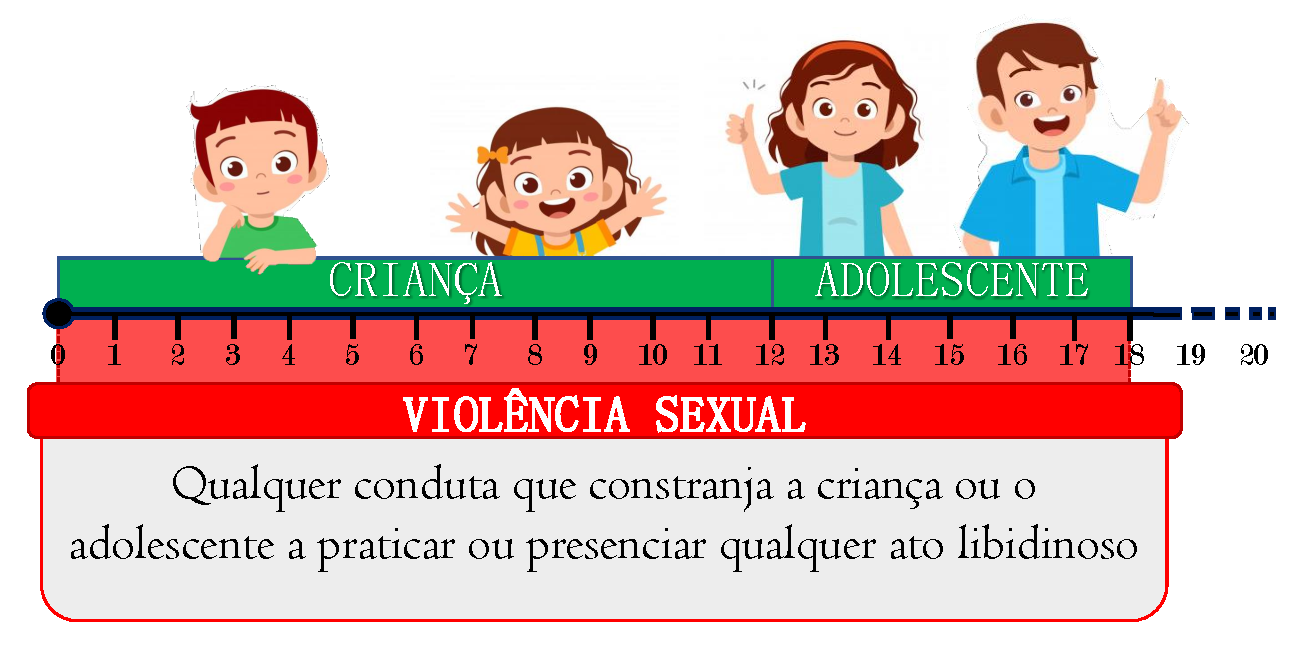
\includegraphics[width=\textwidth]{./Visuais/DefinicaoViolencia.pdf}
	\fonte{Elaborada pelo autor (2020).}
\end{figure}

A \autoref{fig:DefinicaoViolencia} define os termos: criança, adolescente e violência sexual. Os termos apresentados são retratados com base nas definições jurídicas brasileiras. No Brasil, de acordo com o \ac{ECA}, compreende-se como \textbf{criança} todo indivíduo até 12 (doze) anos de idade incompletos e como \textbf{adolescente} todo o indivíduo entre 12 (doze) e 18 (dezoito) anos de idade \cite{Lei:8069:1990}. Qualquer conduta libidinosa forçada contra um menor de 18 (dezoito) anos é caracterizada como violência sexual. A legislação brasileira classifica a violência sexual contra as crianças e adolescentes em três categorias: abuso sexual, exploração sexual comercial e tráfico de pessoas \cite{Lei:13431:2017}.

A legislação brasileira considera como \textbf{exploração sexual comercial}, todas as condutas sexuais com menores de idade envolvendo remuneração ou compensação. O conceito de \textbf{tráfico de pessoas} se firma sobre essa definição, englobando todas as atividades coercivas cujo a finalidade seja a exploração sexual. Já o conceito de \textbf{abuso sexual} se assemelha com a definição de \textbf{violência sexual} na legislação brasileira, sendo considerado como abuso sexual de criança ou adolescente, quaisquer atos libidinosos praticados de maneira forçada com um destes grupos, ou ambos. Entende-se como ato libidinoso, toda ação de satisfação da libido do agente agressor ou de outrem \cite{Lei:13431:2017}. Tais atos se dividem em duas categorias, as atividades com contato físico e as atividades sem contato físico. É listado a seguir, um compilado dos principais tipos de abuso sexual encontrados na literatura: 

%\raggedright
\begin{parcolumns}[sloppy, distance=3em, colwidths={2=0.5\textwidth}]{2}
	\colchunk{\flushright \underline{Abuso sexual \textbf{sem} ($\times$) contato físico}}
	\colchunk{\flushright \underline{Abuso sexual \textbf{com} (\checkmark) contato físico}}
	\colplacechunks

	\colchunk{\begin{itemize}[leftmargin=0.5cm]\item[$\times$] \justify \textbf{Abuso sexual verbal:} consiste em conversas abertas sobre atividades sexuais, destinadas a despertar o interesse da criança ou chocá-la.\end{itemize}}
	\colchunk{\begin{itemize}[leftmargin=1.8cm]\item[\checkmark] \justify \textbf{Estupro:} prática sexual forçada envolvendo penetração vaginal ou anal, ou quaisquer outras formas de abuso sexual com contato físico.\end{itemize}}

	\colplacechunks

	\colchunk{\begin{itemize}[leftmargin=0.5cm]\item[$\times$] \justify \textbf{Exibicionismo:} consiste em mostrar os órgãos genitais para crianças ou adolescentes.\end{itemize}}
	\colchunk{\begin{itemize}[leftmargin=1.8cm]\item[\checkmark] \justify \textbf{Sexo oral:} atividade sexual envolvendo contato entre a boca e os órgãos genitais (felação ou cunilíngua).\end{itemize}}

	\colplacechunks

	\colchunk{\begin{itemize}[leftmargin=0.5cm]\item[$\times$] \justify \textbf{Voyeurismo:} observar as genitálias da criança contra a vontade dela.\end{itemize}}
	\colchunk{\begin{itemize}[leftmargin=1.8cm]\item[\checkmark] \justify \textbf{Masturbação:} estimulação manual dos órgãos genitais da criança.\end{itemize}}

	\colplacechunks

	\colchunk{\begin{itemize}[leftmargin=0.5cm]\item[$\times$] \justify \textbf{Grooming:} consiste no aliciamento de crianças por meios eletrônicos.\end{itemize}}
	\colchunk{\begin{itemize}[leftmargin=1.8cm]\item[\checkmark] \justify \textbf{Aliciamento sexual:} suborno sexual mediante dinheiro ou poder.\end{itemize}}

	\colplacechunks

	\colchunk{\begin{itemize}[leftmargin=0.5cm]\item[$\times$] \justify \textbf{Sexting:} compartilhamento de conteúdo erótico por meios eletrônicos.\end{itemize}}
	\colchunk{\begin{itemize}[leftmargin=1.8cm]\item[\checkmark] \justify \textbf{Importunação sexual:} ato sexual sem a anuência dos envolvidos.\end{itemize}}
\end{parcolumns}

\newpage

A literatura revela uma quantidade expressiva de práticas sexuais abusivas \cite{brasil2002notificacao, habigzang2005abuso, sayao2006refazendo, santos2011guia, ibiapina2013influencias, lima2013violencia, lima2015violencia, barros2016participaccao, brasil2018violencia}. Salienta-se neste sentido, que outros tipos de abuso sexual não listados por este trabalho encontram-se devidamente documentados na literatura base. Existe inclusive uma compreensão mais ampla de abuso sexual com contato físico em alguns estudos, que inclui contatos forçados como beijos e toques em algumas zonas corporais erógenas \cite{sayao2006refazendo, santos2009guia}.

No Brasil, os atos praticados ou tentados de abuso sexual são punidos pela legislação brasileira. Eles podem ser legalmente tipificados em: rufianismo, corrupção de menor, assédio sexual, estupro de vulnerável, dentre outros \cite{Lei:12015:2009}. Destaca-se que diferentemente do crime de \textbf{estupro}, que exige constrangimento mediante violência ou grave ameaça, o \textbf{estupro de vulnerável} é crime mesmo com o consentimento da vítima, sendo considerado vulnerável, todo menor de 14 (catorze) anos ou pessoa incapacitada de oferecer qualquer tipo de resistência. 

A idade de 14 (catorze) anos estabelece a idade de consentimento mínima para a consumação de relações sexuais no Brasil. Enfatiza-se, no entanto que não há consenso entre os países acerca a idade de consentimento, podendo variar de região para região \cite{waites2005age}. Em alguns países o consentimento se configura no momento do matrimônio, independentemente da idade e anuência dos nubentes. 

Os atos consumados de abuso sexual são capazes de sequelar suas vítimas tanto fisicamente, quanto emocionalmente. Além disso, uma criança violentada pode chegar em sua fase adulta apresentando os mais variados transtornos e distúrbios \cite{mariscal2003programa, OMS2017responding}. Um achado das principais sequelas do abuso sexual, retratado pela bibliografia na área, é elencado a seguir:

%\raggedright
\begin{parcolumns}[sloppy, distance=3em, colwidths={2=0.35\textwidth}]{2}
	\colchunk{\flushleft \hspace{0.4cm} \underline{Sequelas \textbf{fisiológicas} ($\bullet$)}}
	\colchunk{\flushleft \underline{Sequelas \textbf{comportamentais} ($\circ$)}}
	\colplacechunks
	
	\colchunk{\begin{itemize}[leftmargin=0.5cm]\item[$\bullet$] \justify Gravidez\end{itemize}}
	\colchunk{\begin{itemize}[leftmargin=0.0cm]\item[$\circ$] \justify Depressão\end{itemize}}
	
	\colplacechunks
	
	\colchunk{\begin{itemize}[leftmargin=0.5cm]\item[$\bullet$] \justify Hemorragia\end{itemize}}
	\colchunk{\begin{itemize}[leftmargin=0.0cm]\item[$\circ$] \justify Retraimento\end{itemize}}

	\colplacechunks
	
	\colchunk{\begin{itemize}[leftmargin=0.5cm]\item[$\bullet$] \justify Hematomas\end{itemize}}
	\colchunk{\begin{itemize}[leftmargin=0.0cm]\item[$\circ$] \justify Ideação suicida\end{itemize}}

	\colplacechunks
	
	\colchunk{\begin{itemize}[leftmargin=0.5cm]\item[$\bullet$] \justify Lesões anais\end{itemize}}
	\colchunk{\begin{itemize}[leftmargin=0.0cm]\item[$\circ$] \justify Distúrbios do sono\end{itemize}}
	
	\colplacechunks
	
	\colchunk{\begin{itemize}[leftmargin=0.5cm]\item[$\bullet$] \justify Incontinência anal\end{itemize}}
	\colchunk{\begin{itemize}[leftmargin=0.0cm]\item[$\circ$] \justify Enurese e encoprese\end{itemize}}
	
	\colplacechunks
	
	\colchunk{\begin{itemize}[leftmargin=0.5cm]\item[$\bullet$] \justify Lesões geniturinárias\end{itemize}}
	\colchunk{\begin{itemize}[leftmargin=0.0cm]\item[$\circ$] \justify Transtorno alimentar\end{itemize}}
	
	\colplacechunks
	
	\colchunk{\begin{itemize}[leftmargin=0.5cm]\item[$\bullet$] Infecções sexualmente transmissíveis\end{itemize}}
	\colchunk{\begin{itemize}[leftmargin=0.0cm]\item[$\circ$] \justify Onanismo compulsivo\end{itemize}}
\end{parcolumns}

A bibliografia retrata uma quantidade significativa de traumas recorrentes de eventos sexuais abusivos \cite{OMS2003guidelines, mariscal2003programa, santos2011guia, pavao2013impasse, acuna2014abuso, deslandes2016atendimento}. Informa-se neste contexto, que demais sequelas não elencadas neste trabalho encontram-se devidamente documentadas na literatura da área. Há inclusive registros que relatam como consequência do abuso sexual na infância: agressividade, delinquência, autoflagelação, hipervigilância, hipovigilância, drogadição, estresse pós-traumático, transtorno do pânico e até mesmo a morte \cite{meurer2017direitos}. 

As sequelas do abuso sexual variam com base em certas condições, dentre elas: a idade da criança no início da violência; a duração e quantidade de ocorrências do abuso; o nível da violência; a diferença de idade entre os envolvidos e o vínculo entre criança e agressor \cite{florentino2015possiveis}. A maneira como essas condições ocorrem influenciam diretamente nos efeitos trágicos do abuso, isso pois, para as crianças menores, os sintomas tendem a se agravar mais devido a disparidade de tamanho entre os órgãos da criança e os órgãos do agressor. Além disso, a alta maleabilidade do encéfalo infantil permite que experiências negativas tenham maior probabilidade de causar danos graves e permanentes ao indivíduo \cite{pereira2011crescimento}. Registros informam inclusive que cerca de 90\% das pessoas com problemas psiquiátricos, sofreram alguma forma de maltrato na infância, sendo o abuso sexual, a forma de maltrato mais predominante relatada. Embora o abuso sexual seja largamente relatado em indivíduos com problemas psiquiátricos, é importante destacar que algumas crianças passam pelo abuso sem apresentar as sequelas descritas na literatura especializada \cite{aded2006abuso}. 

O abuso sexual de crianças traz consequências para toda civilização. A \ac{OMS} afirma inclusive que o abuso sexual é um grave problema de saúde pública a ser enfrentado por toda a sociedade \cite{OMS2017responding}. Estudos sobre sua incidência e prevalência mostram que esse fenômeno traz consequências que impactam significativamente a qualidade de vida das vítimas e de suas famílias, além de gerar altos custos econômicos para o país \cite{pinto2017avaliaccao}. Em resposta a esse fenômeno, incontáveis iniciativas surgiram ao redor do globo, voltadas à proteção dos direitos das crianças e dos adolescentes \cite{finkelhor2009prevention}.

No Brasil, o combate ao \ac{ASI} assume inúmeras formas, como: campanhas governamentais\footnote{A campanha \textbf{Não engula o choro} é uma iniciativa do estado do Paraná composta por animações e panfletos objetivados a sensibilizar a sociedade sobre o enfrentamento à violência e às violações de direitos das crianças.}, operações policiais\footnote{A \textbf{Operação Luz na Infância} é uma operação policial de âmbito internacional para à prevenção e enfrentamento de crimes cibernéticos relacionados ao abuso e exploração sexual de crianças e adolescentes.} e canais de denúncia\footnote{O \textbf{Disque 100} é um canal de comunicação para denúncias de violação de direitos humanos.}. Todavia, as estratégias do governo brasileiro não parecem surtir efeito no combate ao abuso sexual de crianças e adolescentes. Isso, pois as taxas anuais do abuso sexual mais que dobraram em um período inferior ao de uma década. A \autoref{fig:HistoricoViolencia} ilustra a aparente ineficiência das estratégias governamentais, com os registros da década de 2010 revelando um aumento quase que contínuo nos índices de abuso sexual de crianças e adolescentes.

\begin{figure}[!t]
	%\centering
	\caption{Panorama do Abuso Sexual Infantil, Brasil.}\label{fig:HistoricoViolencia}
    \hspace{-4.8 cm}
    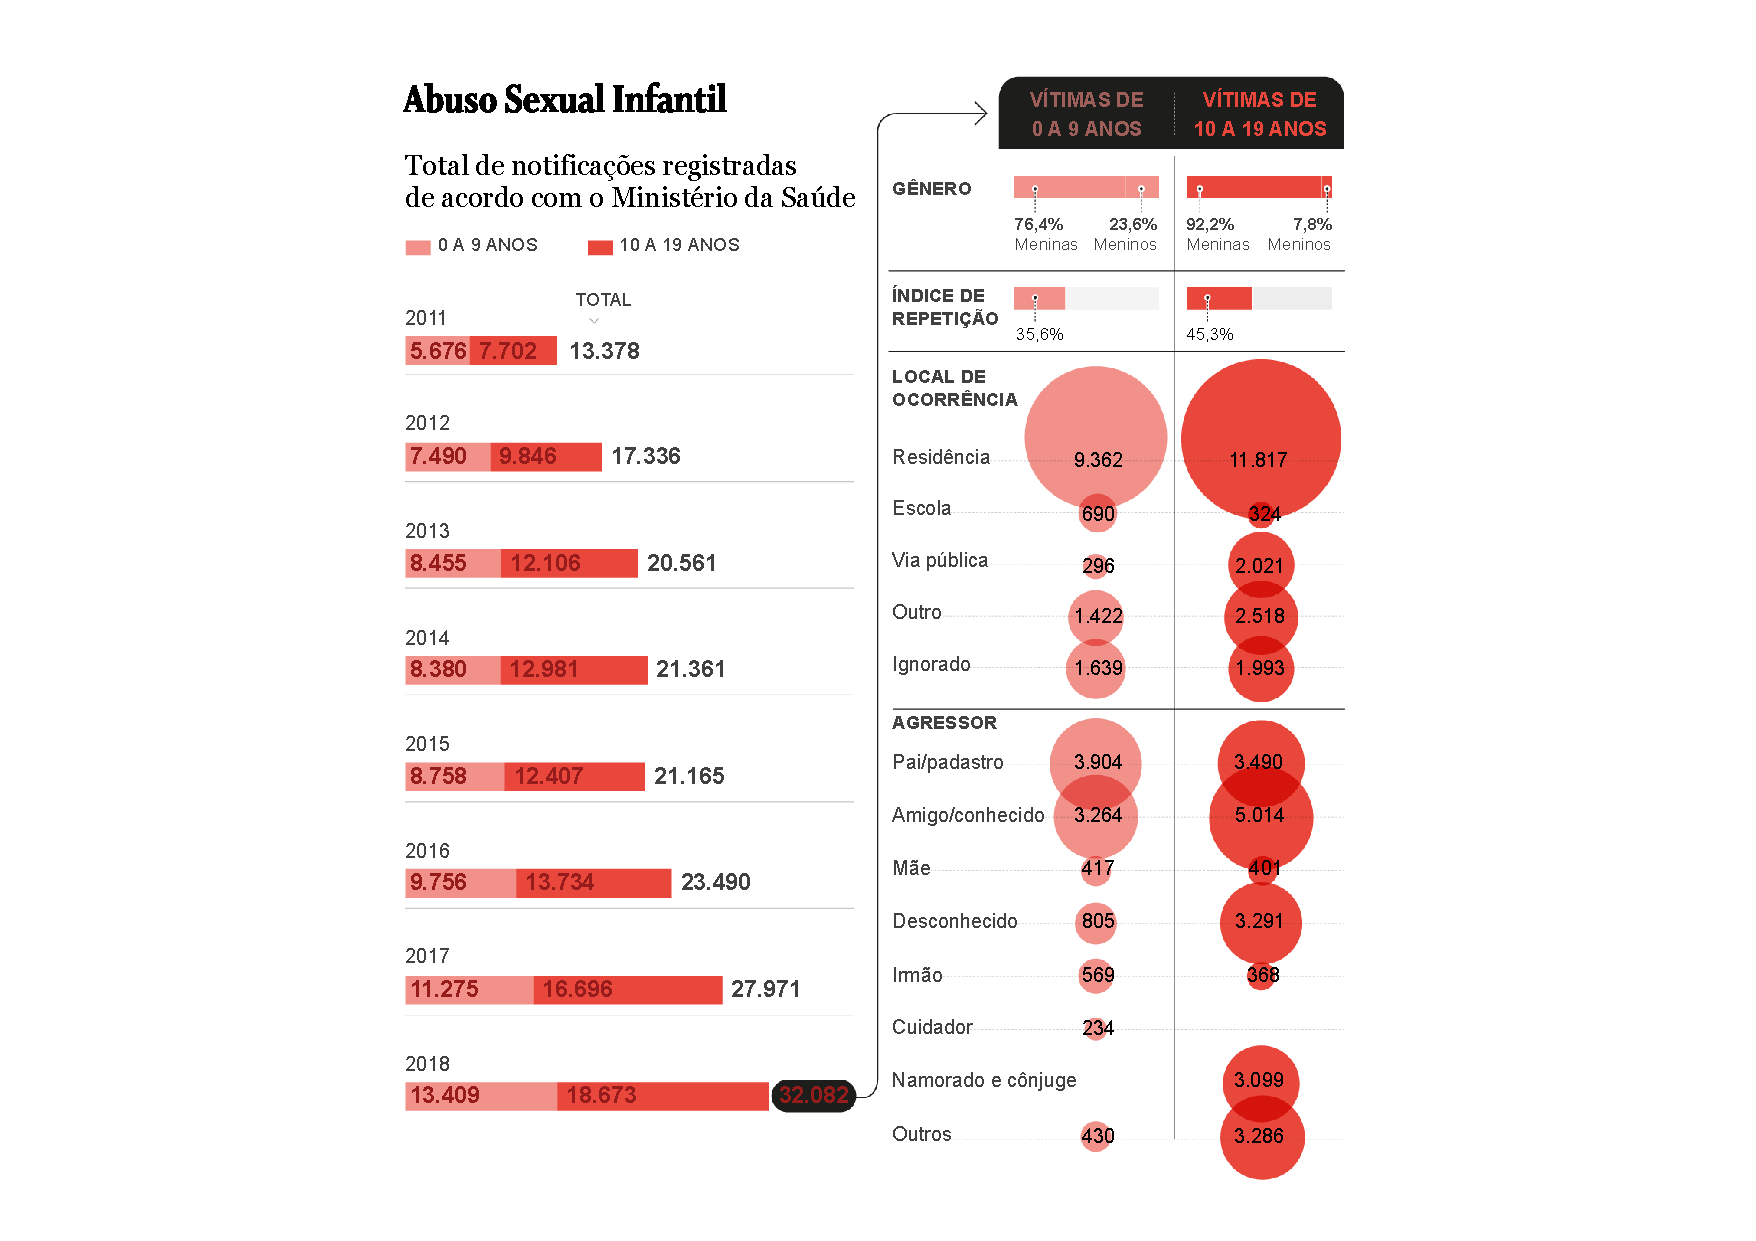
\includegraphics[width=1.6\linewidth]{./Visuais/HistoricoViolencia.pdf}
  	\vspace{-1.0cm}
	\fonte{Adaptado de \citeonline{globo2020tres}.}
\end{figure}

A \autoref{fig:HistoricoViolencia} apresenta a extensão do \ac{ASI} no Brasil. Os dados do DataSus\footnote{O DataSus é um departamento do Ministério da Saúde (MS) com a responsabilidade de coletar, processar e disseminar informações sobre a saúde nacional: \url{https://datasus.saude.gov.br/acesso-a-informacao/doencas-e-agravos-de-notificacao-de-2007-em-diante-sinan/}.} revelam um aumento expressivo na quantidade de notificações de abuso sexual de crianças, adolescentes e jovens adultos, entre os anos de 2011 e 2018. Os dados governamentais, além de apresentarem a totalidade das notificações distribuídas por ano, também filtra seus resultados por gênero, faixa etária, local de ocorrência, agressor, e outros tipos. 

Os dados governamentais demonstram um considerável aumento no número das notificações de violência sexual infantil no intervalo que abrange os anos de 2011 e 2018. Tal aumento pode indicar uma provável ineficiência das estratégias nacionais no combate ao \ac{ASI}. Contudo, cabe destacar que o ano de 2011 marca início de uma portaria\footnote{\label{note:nota0}Portaria Nº 1.171 de 19 de maio de 2011. Art. 2º Fica determinado que todos os estabelecimentos de saúde situados no território nacional, públicos e privados, integrantes ou não do \ac{SUS}, devem informar ao \acf{MS}, por intermédio dos gestores Municipais ou Estaduais, a ocorrência de todas as internações, independente de qualquer que seja a fonte de remuneração dos serviços prestados. Disponível em: \url{https://bvsms.saude.gov.br/bvs/saudelegis/gm/2011/prt1171_19_05_2011_rep.html}.} que obriga os agentes de saúde a notificar ao \ac{MS} todos os atendimentos. A portaria em si, tem como objetivo mitigar a questão da subnotificação dos dados, além de outras questões. Sendo assim, o aumento das notificações de violência sexual infantil após o ano de 2011 poderia ser um resultado da portaria, onde informações que estavam sendo subnotificadas passaram a serem notificadas. Contudo, pesquisas posteriores a portaria apontam que somente 10\% dos casos de violência sexual são notificados às autoridades \cite{brasil2020abuso}. 

A subnotificação faz com que apenas uma parcela do problema seja revelada. O problema do \ac{ASI} manifesta-se então como um \textit{iceberg}, sendo a ponta do \textit{iceberg} a parte conhecida e notificada do problema e a parte submersa do \textit{iceberg} todos os casos não notificados. A subnotificação interfere diretamente na quantificação dos dados e na compreensão da dimensão do problema \cite{deslandes2016atendimento, hora2017violencia}. Dentre os principais motivos da subnotificação cita-se: o medo de represálias, o receio do estigma social, o descrédito dos agentes de saúde (antes da portaria\footref{note:nota0}) e a inscícia infantil \cite{fbsp2019anuario, pavao2013impasse}. %iceberg = geleira?

A inscícia das crianças acaba sendo um fator chave da subnotificação do problema. Em alguns casos a baixa vivência da criança faz com que o menor acabe por interpretar o abuso sexual sofrido com uma manifestação de carinho ou como uma prática normal \cite{aded2006abuso}. Em outros casos existe a inaptidão do menor em realizar o processo de denúncia, com a denúncia não sendo formalizada devido ao desconhecimento do processo legal por parte da criança \cite{OMS2002world}. Além disso, a incompreensão dos tramites legais pode levar a pensamentos incertos no que diz respeito ao sustento da casa, relacionado com seu provedor. As estratégias do governo brasileiro de combate ao \ac{ASI} falham nesse sentido, pois são praticamente incapazes de alcançar uma criança violentada sob estas condições, sendo uma das únicas formas de salvação da criança, a realização da denúncia por um terceiro. Além disso, tais estratégias, comumente se baseiam no princípio que o abuso já tenha ocorrido, enfatizando que a denúncia ainda se faz válida para episódios tentados (ou suspeitos) de abuso sexual.

O \ac{ASI} não é tratado com o rigor necessário pelo governo brasileiro. Grande parte das estratégias nacionais enfrentam o problema do abuso sexual de forma corretiva e não de maneira preventiva. A dificuldade das crianças em manifestar a violência sofrida acaba prejudicando as medidas tomadas pelas organizações nacionais. Sendo assim, uma das formas de contornar este empecilho vem por meio da conscientização de crianças, forma a qual já é aplicada em vários países \cite{plummer1999history, muller2014child}.

O Brasil aplica a conscientização de crianças no combate às drogas. A conscientização é realizada pelo \ac{PROERD}\footnote{O Programa Educacional de Resistência às Drogas e à Violência promove curso de quatro meses, ministrado por policiais militares voluntários, capacitados pedagogicamente, em parceria com pais, professores, estudantes e comunidades. Com ênfase na prevenção ao uso de drogas, as aulas mostram aos estudantes do quinto ano do ensino fundamental das redes pública e particular como se manter longe de más companhias, como evitar a violência, como resistir às pressões diretas ou indiretas e como acionar os pais ou responsáveis quando necessário. Mais informações sobre o programa podem ser encontradas em: \url{http://portal.mec.gov.br/ultimas-noticias/211-218175739/15910-programa-mostra-a-estudantes-como-ficar-longe-das-drogas}.}. Embora a temática da violência seja abordada, a violência sexual não é devidamente tratada pelo programa em questão. Para combater de maneira efetiva o problema do \ac{ASI} no Brasil é necessário a instauração de um programa educacional sólido de prevenção à violência sexual infantil que capacite e conscientize as crianças. 

Inúmeros estudos apontam como consequência benéfica dos programas de prevenção do \ac{ASI} a redução da incidência nos casos de abusos sexuais no médio e longo prazo \cite{maria2010papel}. Uma metanálise internacional informa inclusive que crianças capacitadas por programas do gênero possuem de seis a sete vezes mais chances de apresentarem repulsão a episódios de abuso (simulados) em comparação à crianças não capacitadas \cite{finkelhor2009prevention}. Outros 27 (vinte e sete) estudos revelam também que os programas são eficazes na construção do conhecimento das crianças acerca do abuso sexual e suas habilidades preventivas \cite{collin2013lessons}. 

Iniciativas preventivas de combate ao \ac{ASI} ajudam a evitar a ocorrência de episódios abusivos. Não faltam evidências que comprovam os resultados benéficos dos programas de prevenção e combate ao \ac{ASI} \cite{maria2010papel}. Diante deste fato, implementar um programa de educação nas escolas que prepare as crianças a coibir o abuso sexual é uma excelente maneira de prevenir abusos contra crianças e adolescentes \cite{santos2009guia}. Todavia, a temática do abuso sexual é extremamente sensível e delicada. A tarefa de ministrar tal conteúdo em salas de aula, pode acabar se tornando uma tarefa árdua e complicada. Como facilitador, surgem as estratégias pedagógicas baseadas em jogos. 

Estratégias baseadas em jogos didáticos vêm a agregar e facilitar o aprendizado infantil, principalmente em temas difíceis de abordar, devido aos tabus e aos preconceitos que os permeiam \cite{miranda2018abordagem}. As abordagens baseadas em jogos trazem diversão para temáticas sensíveis e pesadas, deixando os conteúdos apresentados e ensinados menos desagradáveis e incômodos. 

Jogos didáticos fornecem um meio poderoso de aprendizagem proporcionando uma maior motivação, confiança, engajamento e envolvimento dos alunos na aprendizagem, além de garantir um aprimoramento de suas habilidades \cite{colleen2016advancing}. Jogos associados a educação apresentam uma série de benefícios e vantagens. Entretanto, trazem algumas desvantagens como custos associados a produção, manutenção e treinamento. Como forma de contornar estes gastos, surgiram os jogos didáticos digitais.

\pagebreak

Os jogos didáticos digitais são ótimos facilitadores do processo pedagógico, pois herdam todas as vantagens associadas aos jogos físicos, sem herdar totalmente suas desvantagens. O principal empecilho que surge no lugar, diz respeito ao alcance dos jogos digitais. Em um cenário como o do Brasil, os jogos didáticos digitais enfrentam barreiras tecnológicas e econômicas. Um jogo didático digital, requer que o jogador possua um aparelho compatível com o jogo e conexão com a \textit{internet} (além de energia elétrica). A conexão com a \textit{internet} se faz necessária para o envio de informações sobre o desempenho do jogador no jogo a um banco de dados. Visando minimizar essas barreiras, soluções tecnológicas surgiram, como os jogos para navegadores. 

Os jogos para navegadores diminuem os requisitos necessários para a execução de um jogo. Entretanto, uma conexão via servidor ainda se faz indispensável neste tipo de aplicação na qual a coleta remota dos dados do jogador é necessária. Felizmente, o Brasil tem ampliado cada vez mais o número de indivíduos conectados à \textit{internet}. Em 2019, a porcentagem de crianças e adolescentes conectados à rede alcançava os 89\% de toda essa população (entre nove e dezessete anos) \cite{nic2019pesquisa}. A expansão do número de usuários conectados à rede, viabiliza a instauração de um programa nacional preventivo de combate ao \ac{ASI} totalmente baseado na ideia de jogos para navegadores. Há inclusive, registro em vários países, de jogos do gênero sendo aplicados com sucesso na prevenção e no combate da violência sexual de crianças e adolescentes \cite{jones2008online, fingerle2018abschlussbericht}. 

Os jogos para navegadores voltados à prevenção e ao combate à violência sexual infantil, demonstram sucesso expressivo no ensino de habilidades preventivas. Os conceitos abordados por tais jogos assumem um importante papel no combate à violência sexual infantil. A oportunidade das crianças em praticar tais conceitos por intermédio de jogos fortalece ainda mais a luta contra os maus-tratos de meninas e meninos \cite{collin2013lessons}. A abordagem preventiva por meio de jogos digitais demonstra-se promissora no combate desse problema que assola tanto o Brasil, quanto o mundo. 

O enfretamento e a efetiva diminuição no número de casos de \ac{ASI} pode ser alcançado por intermédio de jogos educacionais para navegadores com temática preventiva a violência sexual infantil. Contudo, para isso, se faz necessário que tais jogos cumpram com certos requisitos, a fim de comprovar seus benefícios e justificar sua utilização por crianças de modo geral \cite{campos1996dez}. Sendo assim, jogos educacionais devem passar por um processo avaliativo para que sua eficácia pedagógica seja constatada, averiguando desta forma, se cada lição do jogo consegue cumprir com aquilo que foi planejado para ele \cite{montilva2002method, padron2007towards}. No caso de jogos com temática sensível, um processo avaliativo devidamente conduzido é capaz também de auxiliar na identificação de eventuais desconfortos que um jogo possa causar. Um jogo que seja rejeitado pelo processo avaliativo deve ter seu desenvolvimento retomado para corrigir eventuais falhas constatadas. Entretanto, um jogo de caráter preventivo à violência sexual infantil, aprovado pelo processo avaliativo, possui grande potencial para fortalecer os esforços na luta contra a violência sexual de crianças e adolescentes. 

%O correte trabalho observa a questão da violência sexual. O problema é estudado, analisado e devidamente delimitado, conforme a metodologia científica determina. A análise dos dados revelou que mais de metade dos casos de violência sexual são cometidos contra menores de idade (\autoref{fig:HistoricoViolencia}). Por tal razão, o problema em si, foi delimitado pela correte pesquisa de modo a se conscentar na violência infantil. Além disso, o problema foi delimitado em termos de soluções, onde as soluções baseadas em jogos demonstraram-se pertinentes para atuar sobre o problema. Desta forma, a atual pesquisa desenvolve um jogo digital de caráter preventivo a questão da violência sexual infantil. O jogo assenta seu desenvolvido em conceitos e estratégias encontradas nas bases da literatura pesquisa. Buscando averiguar a eficácia do pedagógica do jogo, a atual pesquisa realiza experimentos com um amostra de crianças. Espera-se que a implementação de tal estratégia impacte, a curto prazo, nas habilidades e nos conhecimentos das crianças envolvidas no programa. A longo prazo, conjectura-se que haja uma diminuição das taxas de violência sexual infantil a nível nacional. 

%A presente dissertação organiza sua redação em sete capítulos. O \autoref{ch:Introducao} dá uma breve descrição sobre a problemática a ser abordada, os objetivos da pesquisa e sua metodologia. O \autoref{ch:Fundamentacao} fundamenta algumas ideias essenciais para a compreensão e andamento da pesquisa, abordando desde a definição de Jogo Sério, metodologias para o desenvolvimento de jogos e modelos para a avaliação de programas voltados para a prevenção da violência sexual infantil. O \autoref{ch:Relacionados} apresenta algumas estratégias voltadas para o combate da violência sexual de crianças. O \autoref{ssec:TR} apresenta os trabalhos relacionados com a atual pesquisa. O \autoref{ch:Desenvolvimento} ilustra as questões de desenvolvimento do jogo elaborado, desde aspectos técnicos até aspectos pedagógicos. O \autoref{ch:Avaliacao} explica o processo de validação do jogo. Por fim, o \autoref{ch:Conclusao} finaliza a atual pesquisa com suas conclusões.


%-------------------------------------------------------------------------------------------------------------------
\newpage
\section{Objetivos}\label{sec:Objetivos}

A presente pesquisa identificou a necessidade de implementar propostas de estratégias no combate à violência sexual infantil. Nacionalmente, existem propostas de estratégias semelhantes as existentes no exterior, as quais apresentam grande sucesso \cite{steiler2012orbit, jones2020serious}. A atual pesquisa acredita que uma estratégia totalmente nacional devidamente adaptada a cultura e a realidade brasileira possui maiores chances de sucesso, em frente a uma estratégia estrangeira importada. Por tal razão, a presente pesquisa assenta suas ideias com base na estratégia educativa nacional proposta por \citeonline{diocesano2018infancia}.

\citeonline{diocesano2018infancia} propõe um jogo educacional para prevenção da violência sexual infantil, denominado de \textbf{Infância Segura}. O jogo em questão se destaca frente as outras propostas nacionais, pois possui uma quantidade superior de dinâmicas e uma maior variedade de temas tratados. Além disso, as temáticas abordadas pelo jogo proposto por \citeonline{diocesano2018infancia} obedecem a orientações internacionais de educação em sexualidade \cite{unesco2018international}. Sendo assim, essa pesquisa elege o jogo \textbf{Infância Segura} para ser desenvolvido como uma estratégia de combate e prevenção à violência sexual.

Como pesquisa científica, se busca avaliar o jogo desenvolvido por meio de estudos, análises e experimentos. Uma pesquisa científica não diz respeito pura e simplesmente a construção de artefato, mas sim, aos achados e as descobertas envolvendo este artefato \cite{wazlawick2014metodologia}. Deste modo, o jogo desenvolvido configura-se como objetivo específico da presente pesquisa, já a avaliação deste jogo configura-se como objetivo geral do atual trabalho acadêmico. Para atingir o objetivo geral, conjecturou-se o \hyperref[hipotese]{seguinte} teste de hipótese:

\label{hipotese}
\begin{itemize}
	%\item \textbf{Hipótese Nula (H$_{0}$):} O conhecimento de crianças, sobre a prevenção da violência sexual, é mantido após serem submetidas ao programa educacional desenvolvido nessa pesquisa, tendo como comparação seus desempenhos na etapa de pré e pós-teste. 

	%\item \textbf{Hipótese Alternativa (H$_{1}$):} O conhecimento de crianças, sobre a prevenção da violência sexual, é ampliado após serem submetidas ao programa educacional desenvolvido nessa pesquisa, tendo como comparação seus desempenhos na etapa de pré e pós-teste.
	\item \textbf{Hipótese Nula (H$_{0}$):} O conhecimento sobre a prevenção da violência sexual de crianças, submetidas ao jogo desenvolvido nessa pesquisa (grupo experimental), não apresenta diferenças estatísticas significativas entre os conhecimentos sobre prevenção de crianças não submetidas ao jogo desenvolvido (grupo controle).
	
	\item \textbf{Hipótese Alternativa (H$_{1}$):} O conhecimento sobre a prevenção da violência sexual de crianças, submetidas ao jogo desenvolvido nessa pesquisa (grupo experimental), é estatisticamente superior aos conhecimentos sobre prevenção de crianças não submetidas ao jogo desenvolvido (grupo controle). 
\end{itemize}


%\legend{\large\label{hipotese}\Large{\textbf{Hipótese de pesquisa}}}
%\begin{framed}
%	\noindent
%	{\fontfamily{cmr}\selectfont O programa educacional para a prevenção da violência sexual infantil desenvolvido nessa pesquisa gera, aos participantes do programa, uma resposta cognitiva sobre os conceitos abordados.}
%\end{framed}


As \hyperref[hipotese]{hipóteses apresentadas} visam validar ou invalidar o jogo desenvolvido por esse trabalho como uma proposta de combate à violência sexual infantil. A avaliação do jogo define o objetivo geral (objetivo primário) da atual pesquisa acadêmica. Já o seu desenvolvimento configura o objetivo específico (objetivo secundário) do atual trabalho. O processo de avaliação do jogo é descrito em maiores detalhes na \autoref{sec:Avaliativos}. Enquanto que o jogo em si é descrito no \autoref{ch:Desenvolvimento}. Os resultados desta pesquisa, relacionados as \hyperref[hipotese]{hipóteses} apresentadas, são documentados no \autoref{ch:Avaliacao}.

%-------------------------------------------------------------------------------------------------------------------

\section{Delimitação}\label{sec:Escopo}

A atual pesquisa fundamenta seus alicerces no desenvolvimento e na avaliação de um jogo para prevenção da violência sexual infantil. O jogo desenvolvido pelo corrente trabalho tem o intuito de ensinar à prevenção da violência sexual infantil para crianças entre 5 (cinco) e 8 (oito) anos de idade. A faixa etária estabelecida para o jogo segue as orientações internacionais da \ac{UNESCO}\footnote{O documento da UNESCO separa os conceitos pedagógicos em quatro faixas etárias distintas (5 a 8 anos; 9 a 12 anos; 12 a 15 anos e 15 a 18+ anos). A \ac{UNESCO} recomenda que para maximizar a aprendizagem, é necessário trabalhar tópicos múltiplos relativos à sexualidade de maneira apropriada para a idade no decorrer de vários anos, utilizando uma abordagem de currículo em espiral. O documento pode ser acessado por meio do seguinte endereço eletrônico: \url{https://unesdoc.unesco.org/ark:/48223/pf0000369308}.}. No mais, a faixa etária estabelecida por esse trabalho foca em um dos grupos etários mais violentados de acordo com as pesquisas (\autoref{fig:violeciaIdade}). Além disso, é nessa faixa etária que programas de prevenção são mais eficazes \cite{davis2000child}.

\begin{figure}[htb]
	%\centering
	\caption{Taxa de vítimas de estupro, por faixa etária, Brasil (2020).}\label{fig:violeciaIdade}
    \frame{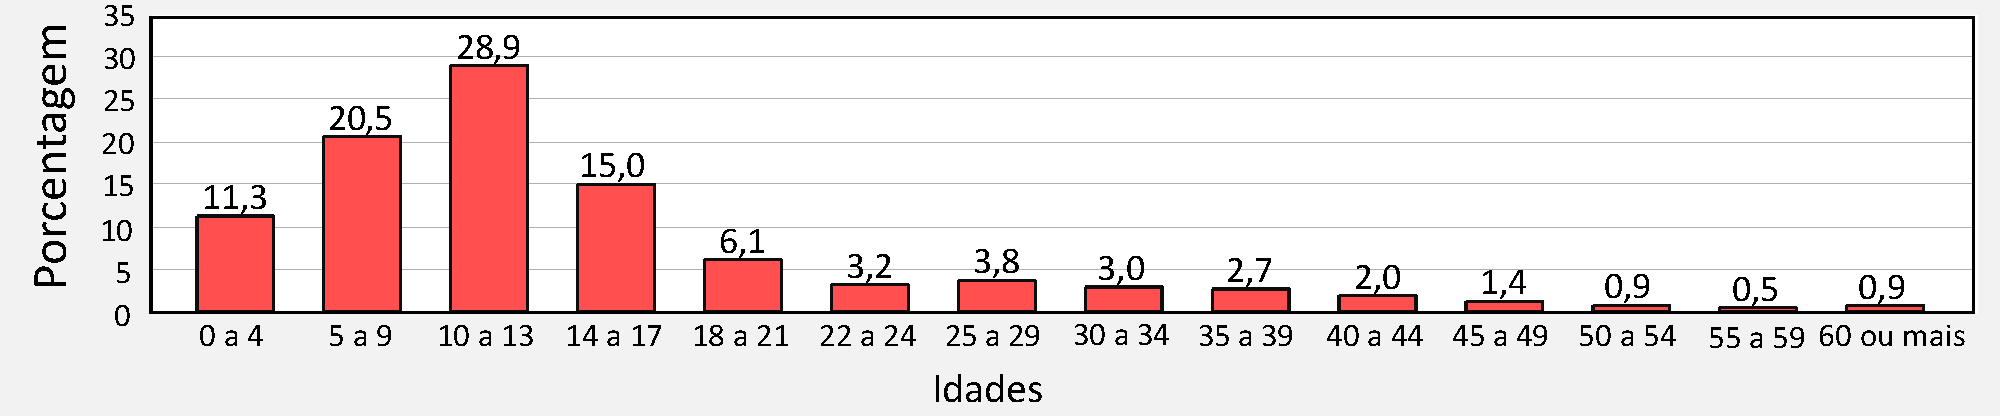
\includegraphics[width=\linewidth]{./Visuais/Idades1.pdf}}
	\fonte{\citeonline[p. 113]{fbsp2021anuario}.}
	\vspace{-0.3cm}
\end{figure}


%É de notório saber que um programa sólido de educação sexual deve acompanhar a criança e o adolescente até sua fase adulta, contudo o atual trabalho abrange apenas a faixa etária mais tênue definida pela \ac{UNESCO}. A seleção da faixa etária mais tênue se deve pelo fato desta demarcar o início e a primeira etapa para os programas de educação sexual. Além disso, os prazos estabelecidos impedem que as demais etapas possam ser abordadas por essa pesquisa com a devida cautela e cuidado. Por tal razão, cabe a trabalhos futuros o desenvolvimento das demais etapas.

A presente pesquisa estabelece uma abordagem pedagógica baseada em um jogo educativo para prevenção da violência sexual infantil. Abordagens pedagógicas voltadas a prevenção da violência sexual infantil por meio de jogos já possuem resultados promissores em vários países \cite{muller2014child, fingerle2018abschlussbericht}. Além disso, tal abordagem ainda proporciona um sistema competente de acesso a informações positivas, confiáveis e livre de julgamentos sobre sexualidade e relacionamentos \cite{unesco2018international}. %Desta forma, a abordagem por intermédio de jogos é eleita pela presente pesquisa para contemplar um programa educacional de prevenção a violência sexual infantil. 

O jogo desenvolvido por essa pesquisa assenta seus conceitos pedagógicos e técnicos em documentos da literatura científica na área. Salienta-se que não se mensurou-se a efetiva contribuição de cada aspecto no processo de aprendizagem ou no processo técnico de desenvolvimento/avaliação. Os materiais usados para a elaboração, implementação e avaliação do jogo desenvolvido não são julgados pela corrente pesquisa, sendo nesse sentido, o único papel do presente trabalho acadêmico o de cumprir com as normas e diretrizes dos materiais base utilizados. 

%Em virtude da sensibilidade da temática tratada e do público-alvo vulnerável do corrente trabalho, informa-se da necessidade desta pesquisa em passar pelo Comitê de Ética. Após a aprovação da banca, os devidos tramites legais serão tomados para submeter essa pesquisa aos protocolos éticos cabíveis. 

Em virtude da sensibilidade da temática tratada e do público alvo vulnerável do corrente trabalho, informa-se que os procedimentos técnicos da presente pesquisa, envolvendo seres humanos (descritos na \autoref{sec:Avaliativos}), foram validados pelo Comitê de Ética em junho de 2021, sob o \ac{CAAE} nº 43602921.2.0000.0118 (\refanexo{chap:Aprovacao}). %https://www.udesc.br/arquivos/cct/id_cpmenu/1024/dissertacao_final_15167050734725_1024.pdf
% e seguiu as recomendações éticas vigentes, sobretudo guiadas pela Resolução 466/2012.

%-------------------------------------------------------------------------------------------------------------------
\newpage
\section{Metodologia da Pesquisa}\label{sec:Metodologia}

Para a construção dos conhecimentos desta pesquisa, se faz necessário definir um método a ser seguido. A seção de metodologia da pesquisa surge para trazer maior transparência aos processos e procedimentos que hão de culminar na conclusão de uma determinada pesquisa. Entender e classificar o tipo de pesquisa feita é fundamental para sustentar o planejamento e às decisões tomadas.

O presente trabalho classifica a corrente pesquisa com base nas classificações mais frequentes observadas em pesquisas atuais na área da ciência da computação. Deste modo a subseção \ref{sub:Natureza} menciona a natureza da atual pesquisa, a subseção \ref{sub:Recorte} delineia o tempo desta pesquisa, a subseção \ref{sub:Literatura} apresenta o método de revisão da literatura utilizado pela corrente pesquisa, a subseção \ref{sub:Abordagem} dá sua abordagem, a subseção \ref{sub:Metodo} detalha o método científico utilizado, a subseção \ref{sub:Procedimentos} explica seus procedimentos, a subseção \ref{sub:Finalidade} conta sua finalidade, a subseção \ref{sub:Maturidade} define o grau de maturidade e por fim, a subseção \ref{sub:Considerar} dá as considerações finais da atual seção. 


\subsection{Natureza}\label{sub:Natureza}

A natureza de um projeto de pesquisa vislumbra sobre o seu impacto na sociedade. Há, portanto, duas classificações: pesquisas básicas e pesquisas aplicadas. Pesquisas de natureza básica buscam o enriquecimento teórico do corpo científico. Já as pesquisas de natureza aplicada buscam por soluções para determinados problemas pragmáticos \cite{zanella2006metodologia}.

O corrente trabalho acadêmico almeja solucionar o problema da violência sexual infantil no Brasil. A solução pensada assume a forma de um jogo educacional infantil focado na ensino-aprendizagem sobre a prevenção da violência sexual infantil. Espera-se que o jogo capacite seus jogadores de modo a coibirem e relatarem episódios de abuso culminando assim, na redução dos crimes. Do ponto de vista científico, o jogo em si é um mero produto da presente pesquisa (\textit{e.g.} a indústria de jogos desenvolve inúmeros jogos todos os anos, e isso não significa fazer ciência). O atual trabalho alcança o \textit{status} de pesquisa científica no momento que o jogo em si é posto a prova, de modo a validá-lo ou invalidá-lo como proposta educativa. Definido o problema pragmático a ser tratado, afirma-se que a corrente pesquisa é de natureza aplicada.

\subsection{Recorte}\label{sub:Recorte}

O recorte de um estudo define a duração da pesquisa, podendo ser transversal ou longitudinal. Pesquisas transversais demarcam os estudos realizados em pontos específicos no tempo. Pesquisas longitudinais englobam um intervalo de tempo maior, analisando o durante, o antes e o depois da pesquisa \cite{hochman2005desenhos}. 

O corrente estudo opera em uma janela curta de tempo. As informações analisadas dizem respeito pura e simplesmente a dados colhidos durante o andamento do estudo, por tal razão a atual pesquisa remete a um recorte transversal no tempo. 

\subsection{Revisão da Literatura}\label{sub:Literatura}

A revisão da literatura diz respeito a pressupostos teóricos que dão fundamentação à pesquisa e as contribuições proporcionadas por investigações anteriores \cite{carlos2002elaborar}. Existem duas classificações nesse sentido: as tradicionais e as sistemáticas. As revisões tradicionais não utilizam critérios explícitos para a seleção das obras que hão de fundamentar a pesquisa. Já as revisões sistemáticas são as pesquisas que se utilizam de um processo rigoroso para a seleção de obras para sua fundamentação \cite{ferenhof2016desmistificando}.

O atual estudo conduz uma revisão da literatura tradicional, isenta de quaisquer critérios mais severos para a seleção de artigos. No entanto, o presente trabalho priorizou utilizar os seguintes \acfp{MBA}: ACM DL, IEEExplore, Science Direct e Web of Science. A escolha por esses \acp{MBA} deu-se por obrigarem publicações de qualidade reconhecida pela \ac{CAPES}. Também foram pesquisados periódicos, livros, revistas científicas e \textit{sites} de referência na área; além de consultadas as citações referenciadas durante toda a dissertação. Sendo assim, enfatiza-se que a presente pesquisa baseia sua revisão literária em obras científicas e revisadas por pares principalmente; mas também, em documentos e demais materiais sem tratamento prévio retornados durante a etapa de revisão da literatura. 

\subsection{Abordagem}\label{sub:Abordagem}

A abordagem metodológica de uma pesquisa informa a respeito da natureza de suas variáveis. Logo existem as pesquisas de abordagem quantitativa e as de abordagem qualitativa. Pesquisas quantitativas trabalham sumariamente com variáveis numéricas e objetivas. Já as pesquisas qualitativas trabalham majoritariamente com elementos subjetivos e abstratos \cite{carlos2002elaborar}. As pesquisas que contemplam ambos os tipos são categorizadas como pesquisas quanti-qualitativas ou pesquisas mistas. 

A atual pesquisa mensura o desempenho, a aprendizagem e o engajamento dos participantes envolvidos no processo de avaliação de um jogo educacional. O desempenho (quantitativo) é colhido de maneira virtual por meio de arquivos gerados durante os experimentos realizados com o jogo desenvolvido; neste quesito informações como os acertos, erros e os tempos de resposta para os exercícios do jogo são colhidos. A aprendizagem (quantitativo) é mensurada através de um conjunto de questões focadas em medir o nível de conhecimento adquirido pelos participantes do programa. O engajamento (qualitativo) é alcançado por meio de entrevistas e depoimentos em um grupo focal com o intuito de identificar os níveis de agradabilidade do programa ao seu público-alvo. Definidas as variáveis mensuradas, afirma-se que o atual trabalho possui uma abordagem quanti-qualitativa. 

\subsection{Método}\label{sub:Metodo}

Na área da metodologia, o método define a forma de raciocínio lógico que guiará a pesquisa científica. Quatro formas de raciocínio se destacam: indutivo, dedutivo, hipotético-dedutivo e dialético. O método indutivo induz os achados específicos de uma pesquisa para um contexto geral. O método dedutivo deduz os conhecimentos gerais para contextos específicos. O método hipotético-dedutivo diz respeito as pesquisas baseadas em princípios de falseabilidade. O método dialético descreve os fenômenos de uma pesquisa \cite{marconi2003lakatos}.  

A atual pesquisa submete um jogo educativo a um conjunto reduzido de participantes de modo a confirmar ou falsear suas hipóteses. Desta forma pode-se dizer que o presente estudo segue a corrente hipotético-dedutiva.

%A atual pesquisa submete um programa educacional a um conjunto reduzido de participantes. Os resultados do conjunto não podem ser extrapolados para toda a população de maneira a validar ou invalidar a eficácia do programa. Logo, o presente estudo segue a corrente indutiva. 

\subsection{Procedimentos Técnicos}\label{sub:Procedimentos}

A metodologia divide os procedimentos técnicos em dois grupos distintos de coleta de dados. Há os grupos responsáveis pela coleta direta de informações e os responsáveis pela coleta indireta de informações. A coleta indireta de informações tende a ser realizada por pesquisas documentais ou bibliográficas. Já a coleta direta de informações corresponde normalmente a pesquisas experimentais ou etnográficas \cite{cordova2009pesquisa}. 

A atual pesquisa realiza a avaliação de um jogo educacional com o auxílio de dois grupos de participantes, um grupo experimental e um grupo controle. Tal abordagem é associada a pesquisas experimentais. Todavia, salienta-se que os grupos selecionados pelo presente estudo não obedecem a uma distribuição aleatória (um dos fatores principais para a elaboração de pesquisas experimentais sólidas). %O processo avaliativo da presente pesquisa é composto unicamente por crianças da rede pública de ensino. A seleção exclusiva de participantes da rede pública de ensino resulta em um possível viés da pesquisa. 
%Por tal razão a atual pesquisa se enquadra em uma classe de pesquisas experimentais conhecidas como pesquisas quase-experimentais \apud{campbell1979delineamentos}{carlos2002elaborar}.
Pelo fato dos grupos selecionados serem compostos por indivíduos da mesma região e nível educacional (rede pública), a amostra utilizada não pode ser classificada como totalmente aleatória, sendo assim, a atual pesquisa se enquadra na classe das pesquisas quase-experimentais \apud{campbell1979delineamentos}{carlos2002elaborar}.

%POR NÃO TER MUITAS DIFERENÇAS ETNICAS OU SOCIO-ECONOMICAS A AMOSTRA NÃO É ALEATORIO, POR ISSO ESSA É UMA PESQUISA QUASE-EXPERIMENTAL. 

\subsection{Finalidade}\label{sub:Finalidade}

A finalidade de uma pesquisa define a relação entre a pesquisa e um problema. Três relações se destacam: exploratória, descritiva e explicativa. As exploratórias buscam compreender e explorar melhor determinado problema. As descritivas almejam descrever o problema e identificar relações entre variáveis associadas ao problema. As explicativas procuram explicar e determinar os fatores que contribuem para a ocorrência do problema \cite{trivinos2009introduccao}. 

A atual pesquisa relaciona as variáveis de aprendizagem entre o grupo experimental e o grupo controle, se utilizando do Teste \textit{t} (com 95\% de confiança). Como adicional, o presente estudo também relaciona as variáveis de desempenho e aprendizagem a fim de encontrar relações entre o desempenho de determinados indivíduos em um jogo e o aprimoramento de suas habilidades intelectuais no que diz respeito aos assuntos ministrados pelo jogo. Dada a relação das variáveis mensuradas, afirma-se que a corrente pesquisa é de finalidade descritiva.

\subsection{Nível de Maturidade}\label{sub:Maturidade}

A maturidade de uma pesquisa se divide em níveis de acordo com a observabilidade dos resultados em relação aos trabalhos existentes. O primeiro nível não apresenta nenhum comparativo, sendo a pura descrição do objeto estudado. O segundo nível realiza um comparativo empírico entre o objeto de estudo e demais existentes. O terceiro nível se utiliza de métricas novas para conduzir tal comparativo. O quarto nível se utiliza de métricas consolidadas. O quinto e último nível consiste na apresentação de uma teoria consistente sobre o objeto estudado \cite{wazlawick2014metodologia}.%. com as observações de forma coerente.

O presente trabalho acadêmico desenvolve um jogo focado na prevenção da violência sexual infantil. O jogo desenvolvido é confrontado de maneira empírica com os demais jogos já existentes nesse cenário. Uma tabela comparativa é construída para proporcionar ao leitor maior clareza entre o artefato desenvolvido nessa pesquisa e demais já existentes. Desta forma, essa pesquisa alcança o segundo grau de maturidade. 


\subsection{Considerações}\label{sub:Considerar}

As classificações em metodologia permitem sustentar o planejamento e às decisões tomadas pelo corrente trabalho acadêmico. Os métodos e processos presentes no campo da metodologia auxiliam, não apenas na condução da pesquisa pelo pesquisador autor, mas também na análise e na revisão da pesquisa por demais pesquisadores da área.

O processo de classificação da corrente pesquisa, buscou fundamentação nos trabalhos citados nas respectivas subseções. Todavia, enfatiza-se que o processo de classificação, embora fundamentado, não está livre de falhas. Por tal razão, as classificações feitas, não devem ser vistas como absolutas, mas sim, como as classificações consideradas mais apropriadas identificadas pelo autor desta dissertação. Salienta-se que a presente seção buscou, apenas, classificar a presente pesquisa. Todos os procedimentos conduzidos para a realização da pesquisa e dos experimentos são descritos mais detalhadamente nas demais seções e capítulos desta dissertação.

%-------------------------------------------------------------------------------------------------------------------

%\begin{comment}

\section{Estrutura do Trabalho}\label{ch:Estrutura}

A presente dissertação organiza sua redação em sete capítulos. O \autoref{ch:Introducao} dá uma breve descrição sobre a problemática a ser abordada, os objetivos da pesquisa e sua metodologia. O \autoref{ch:Fundamentacao} fundamenta algumas ideias essenciais para a compreensão e andamento da pesquisa, abordando desde a definição de Jogo Sério, metodologias para o desenvolvimento de jogos e modelos para a avaliação de programas voltados para a prevenção da violência sexual infantil. O \autoref{ch:Relacionados} apresenta algumas estratégias voltadas para o combate da violência sexual de crianças. O \autoref{ssec:TR} apresenta os trabalhos relacionados com a atual pesquisa. O \autoref{ch:Desenvolvimento} ilustra as questões de desenvolvimento do jogo elaborado, desde aspectos técnicos até aspectos pedagógicos. O \autoref{ch:Avaliacao} explica o processo de avaliação do jogo. Por fim, o \autoref{ch:Conclusao} finaliza a atual pesquisa com suas conclusões.

%\end{comment}
%-------------------------------------------------------------------------------------------------------------------






\chapter{Fundamentação}\label{ch:Fundamentacao}

A fundamentação teórica é um elemento crucial para a compreensão dos fundamentos teóricos que dão base aos conceitos que permeiam o objeto de estudo em uma determinada pesquisa. O capítulo de fundamentação surge então para munir o pesquisador dos conhecimentos necessários para o andamento e a conclusão de sua pesquisa. Ao mesmo tempo, a fundamentação auxilia outros pesquisadores na identificação das bases do conhecimento teórico que guiaram determinado estudo. 

O corrente estudo tem como cerne a validação de um programa educacional para a prevenção da violência sexual infantil baseado na dinâmica de jogos. Deste modo, a \autoref{sec:JogosSerios} traz fundamentação sobre os jogos na educação. A \autoref{sec:Engenharia} traz alguns conceitos sobre o desenvolvimento de jogos. A \autoref{sec:Avaliativos} discute sobre modelos voltados para a avaliação de programas educacionais na temática de prevenção a violência sexual infantil.

%-------------------------------------------------------------------------------------------------------------------
\vspace{1.0 cm}
\section{Jogos Sérios}\label{sec:JogosSerios}

Jogos com propósitos educacionais existem a várias décadas. Ao longo dos anos, tais jogos tiveram várias denominações e definições. Dentre as denominações, a que melhor define o contexto desta pesquisa é o termo \ac{JS} (em inglês: \textit{Serious Game}), usado pela primeira vez na história em \citeyear{clark1970serious} \cite{djaouti12011origins}. Desde \citeyear{clark1970serious}, o termo passou por inúmeras revisões até alcançar sua definição atual, a qual compreende como \ac{JS}: todos os jogos projetados para uma finalidade principal que não a pura diversão \cite{michael2005serious, laamarti2014overview, carvalho2015aprendizagem}.

A definição atual de \ac{JS} permite identificar que os jogos classificados como sérios antecedem a própria origem do termo. Isso pois, a história conta que antes da década de 70, alguns jogos já eram utilizados para outros propósitos além do entretenimento \cite{wilkinson2015brief}. Salienta-se, no entanto, que o termo não encontra-se verdadeiramente consolidado na literatura científica da área, existindo inclusive várias definições e termos correlatos \cite{pourabdollahian2012serious}.

Para definir melhor o termo \ac{JS} que fundamentará e guiará o andamento do presente estudo, buscou-se separar o conceito e interpretar individualmente as palavras que o compõem. O termo \textbf{Jogo} demarca o conjunto de atividades regidas por uma estrutura de regras focadas na diversão e no entretenimento \cite{kishimoto1994jogo}. Já o termo \textbf{Sério} define um propósito prático a este conjunto de atividades, geralmente sendo pedagógico, comportamental ou motor \cite{schroeder2017wobu, baptista2017jogos}. %(com os Exergames = Jogos Ativos). 
A Figura \ref{fig:JS}, ilustra de forma resumida os conceitos que fundamentam a definição de \ac{JS} do atual trabalho. 

\pagebreak

\begin{figure}[htb]

	\caption{\label{fig:JS}Infrográfico da terminologia Jogo Sério.}\vspace{-0.1cm}
  \hspace{-0.9cm}
  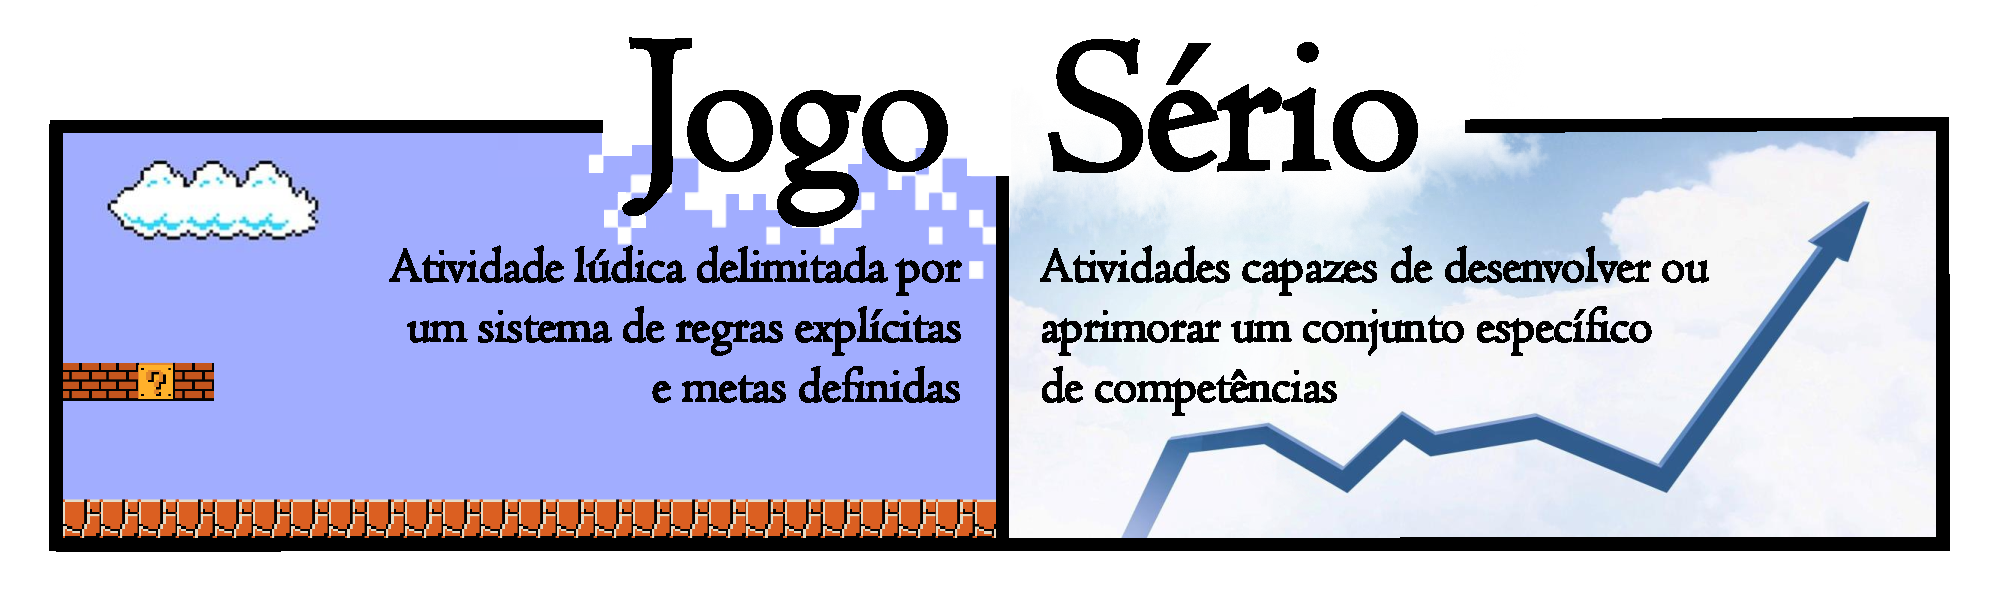
\includegraphics[width=1.1\linewidth]{./Visuais/JogoSerio.pdf}\vspace{-0.1cm}
  \legend{Fonte: Elaborada pelo autor (2020).}

\end{figure}

A Figura \ref{fig:JS} define separadamente a palavra \textbf{Jogo} e \textbf{Sério}. A união das definições dá o conceito de \ac{JS} mais comum encontrado em pesquisas na área \cite{michael2005serious}. Enfatiza-se que para uma atividade se configurar como \textbf{Jogo}, basta obedecer a um conjunto de regras e objetivos. Um jogo nessa definição não precisa de quaisquer outros artefatos para se configurar como tal, podendo ainda, ocorrer individualmente ou coletivamente. Para um jogo abranger o caráter \textbf{Sério} é necessário que o mesmo trabalhe em algum nível as habilidades físicas, comportamentais, ou intelectuais de seus jogadores. 

O aprimoramento ou desenvolvimento de habilidades físicas normalmente é associado aos \textbf{Jogos Ativos} (em inglês: \textit{Exergames}) \cite{araujo2017exergames, schroeder2017wobu}. Já o aprimoramento ou desenvolvimento de habilidades intelectuais é geralmente relacionado aos \textbf{Jogos Educativos}. Pode-se dizer então que a classe de \ac{JS} é uma generalização das áreas de \textbf{Jogos Ativos} e \textbf{Jogos Educativos}. Salienta-se, no entanto, que para um jogo ser classificado como \textbf{Sério}, não se faz necessário que o jogo compreenda ambas as áreas. Todavia, na definição mais aceita, um \ac{JS} deve abranger a área dos \textbf{Jogos Digitais} \cite{laamarti2014overview}.

Os \textbf{Jogos Digitais} são todo o conjunto de jogos, os quais são jogáveis apenas por intermédio de mídias digitais \cite{lucchese2009conceituaccao}. Os jogos digitais, englobam a definição clássica de \textbf{Jogo}, necessitando também de um conjunto de regras e objetivos, porém acrescidos de um motor de jogo e uma interface interativa \cite{battaiola2000jogos}. Enquanto o motor de jogo fica responsável por controlar o conjunto de regras que rege o jogo. A interface interativa se encarrega de converter o jogo em si para sinais visuais e sonoros compreensíveis ao jogador.

Os \textbf{Jogos Digitais}  possuem um sistema de regras mais rígido em relação aos jogos clássicos, devido ao contexto computacional do motor de jogo. O mesmo contexto computacional também é responsável por trazer maior segurança aos \textbf{Jogos Digitais}  em relação aos clássicos, uma vez que a interface interativa é capaz de construir um ambiente lúdico inteiramente virtual, no qual os jogadores possam passar por situações de perigo sem que isso reflita em vias de fato em riscos aos jogadores \cite{lucchese2009conceituaccao}.

Os \acp{JS} assumem um importante papel no aprimoramento das habilidades de seus jogadores à medida que proporcionam um ambiente seguro de interação. Ou seja, \acp{JS} são \textbf{Jogos Digitais}, porém projetados de modo que seus jogadores desenvolvam novas competências e/ou conhecimentos, ou reforcem capacidades existentes \cite{boller2017play}. O contexto digital de tais jogos ainda permite um sistema totalmente livre de julgamentos \cite{unesco2018international}. A depender da dinâmica do jogo, é possível que o jogador interaja com o ambiente virtual do jogo sem que seus erros tenham forte impacto no seu contexto social. Ou seja, o ambiente virtual de um jogo permite aos jogadores um espaço sem pressão social, no qual podem jogar o jogo sem se sentirem acanhados ou tímidos.

Os \acp{JS} proporcionam um sistema de aprendizagem interativa. A aprendizagem interativa é um processo didático de ensino mais atrativo aos \acfp{ND}. Os \acp{ND} apresentam maior preferência por abordagens interativas baseadas em processos de tentativa e erro \cite{pescador2010tecnologias}. Além disso, os \ac{ND} já nascem imersos no mundo digital, o que torna para eles, o processo de iteração com artefatos digitais, um processo mais natural e orgânico, em comparação a iteração entre tais artefatos e os \acfp{ID}.

Os \acp{JS} manifestam-se como um facilitador do processo de aprendizado dos \acp{ND}. A abordagem de \ac{JS} no ambiente escolar pode trazer benefícios ao processo de ensino-aprendizagem, proporcionando um sistema motivador para o desenvolvimento de habilidades cognitivas, além de garantir um sistema de aprendizado por descobertas \cite{carvalho2017move4math}. Um ambiente de aprendizado por descoberta desenvolve o pensamento abstrato dos jogadores, obrigando-os a solucionar problemas inéditos. A solução de problemas inédito é alcançada través de deduções realizadas em comparação a problemas similares apresentados previamente aos jogadores. É crucial que a solução de problemas por meio de \ac{JS} assuma um caráter lúdico que divirta os jogadores na mesma medida que os eduque, para garantir assim, uma maior retenção do conteúdo ensinado \cite{tarouco2004jogos}. 

O presente estudo desenvolve um \ac{JS} objetivado a compor um programa educacional para a prevenção da violência sexual infantil. A compreensão dos fundamentos que definem um \ac{JS} é indispensável para a progressão e conclusão deste trabalho. Buscando trazer maior alcance ao jogo desenvolvido, o jogo em si está exportado para navegadores. Tal característica não fere a definição de \ac{JS}, uma vez que a definição não especifica os meios eletrônicos de acesso ao jogo. Sendo assim, um \ac{JS} para navegadores, permite que um determinando jogo possa ser jogado em qualquer dispositivo com acesso a rede, sem quais restrições mais severas de memória ou processamento. 

O presente trabalho baseia-se nos conceitos pesquisados e nas definições referenciadas nessa seção para fundamentar o \ac{JS} desenvolvido. Não cabe a apresente seção a descrição das temáticas e dos conceitos abordados no jogo. Nesse sentido, salienta-se que a estrutura lúdica e pedagógica do jogo são conceitos abordados por essa dissertação apenas no Capítulo \ref{ch:Desenvolvimento}.

%-------------------------------------------------------------------------------------------------------------------

\section{Metodologia de Desenvolvimento de Jogos}\label{sec:Engenharia}

O mercado de jogos movimenta bilhões de reais todos os anos ao redor do mundo \cite{fortim2020games}. A indústria de desenvolvimento de jogos acompanha essa cifra trazendo cada vez mais pessoas capacitadas para a produção e desenvolvimento de jogos. Em alguns casos o processo de desenvolvimento de um jogo pode envolver milhares de pessoas e levar anos até ser finalizado. Em contrapartida há ainda os jogos de caráter mais independente (\textit{indie game}) que acabam por serems jogos mais modestos em termos de desenvolvimento, se limitando a equipes pequenas, podendo ser produzidos em pouco tempo, ou não. Essa discrepância entre os jogos resulta em uma quantidade variada de metodologias voltadas para o desenvolvimento de jogos.

As metodologias para o desenvolvimento de jogos variam a depender de uma série de fatores. Entretanto, três questões principais são levadas em consideração no momento da escolha por uma metodologia: quantidade de envolvidos no projeto, prazo da entrega e recursos necessários. No mais, após o prazo de entrega, um jogo ainda pode passar por um processo de manutenção trazendo otimizações e customizações ao jogo no decorrer de vários anos. Embora muitos estudos tenham sido publicados sobre o desenvolvimento de jogos para a área da educação, existem poucas metodologias reconhecidas nesta área \cite{aslan2015gamed}. Somado a isso, a literatura informa que o desenvolvimento individual de um produto não precisa necessariamente seguir uma metodologia \cite{valente2021engenharia}. Todavia, no caso do desenvolvimento de jogos educacionais digitais a utilização de uma metodologia é capaz de fornecer uma abordagem estruturada centrada na qualidade do jogo garantindo o cumprimento de objetivos de aprendizagem exigentes no jogo. Sendo assim, o \ac{JS} escolhido pelo presente trabalho para compor um programa de prevenção a violência sexual infantil tem seu desenvolvimento baseado em uma metodologia reconhecida voltada para o desenvolvimento de jogos educativos digitais denominada de \ac{GAMED} \cite{aslan2016digital}. 

A metodologia \ac{GAMED} é uma metodologia voltada para o desenvolvimento de jogos educacionais digitais, podendo ser aplicada tanto para grandes ou pequenos projetos. O \ac{GAMED} apresenta alta qualidade, baixo risco de falhas e alta probabilidade de que o jogo seja concluído dentro do orçamento e prazos estabelecidos \cite{aslan2015gamed}. Além disso, o \ac{GAMED} fornece uma abordagem modular estruturada para superar a complexidade do desenvolvimento e orienta os desenvolvedores durante todo o ciclo de desenvolvimento do jogo.

O \ac{GAMED} é uma metodologia que se incrementa a cada ciclo de desenvolvimento. Ao final de cada ciclo há a entrega de um jogo operacional, por tal razão o \ac{GAMED} pode ser classificado como um método ágil de desenvolvimento. O \ac{GAMED} é constituído por quatro fases principais: Fase de Projeto, Fase de Projeto de \textit{Software}, Fase de Desenvolvimento/Publicação e Fase de Realimentação. As fases são subdivididas em etapas, cada etapa consiste de um processo. A \autoref{fig:GAMED} apresenta um esquema com os principais elementos requeridos no \ac{GAMED}. 

\pagebreak

\begin{figure}[!ht]

	\caption{\label{fig:GAMED}Ciclo de Desenvolvimento de Jogos da Metodologia GAMED.}
  \begin{center}%\vspace{-0.3cm}
    \frame{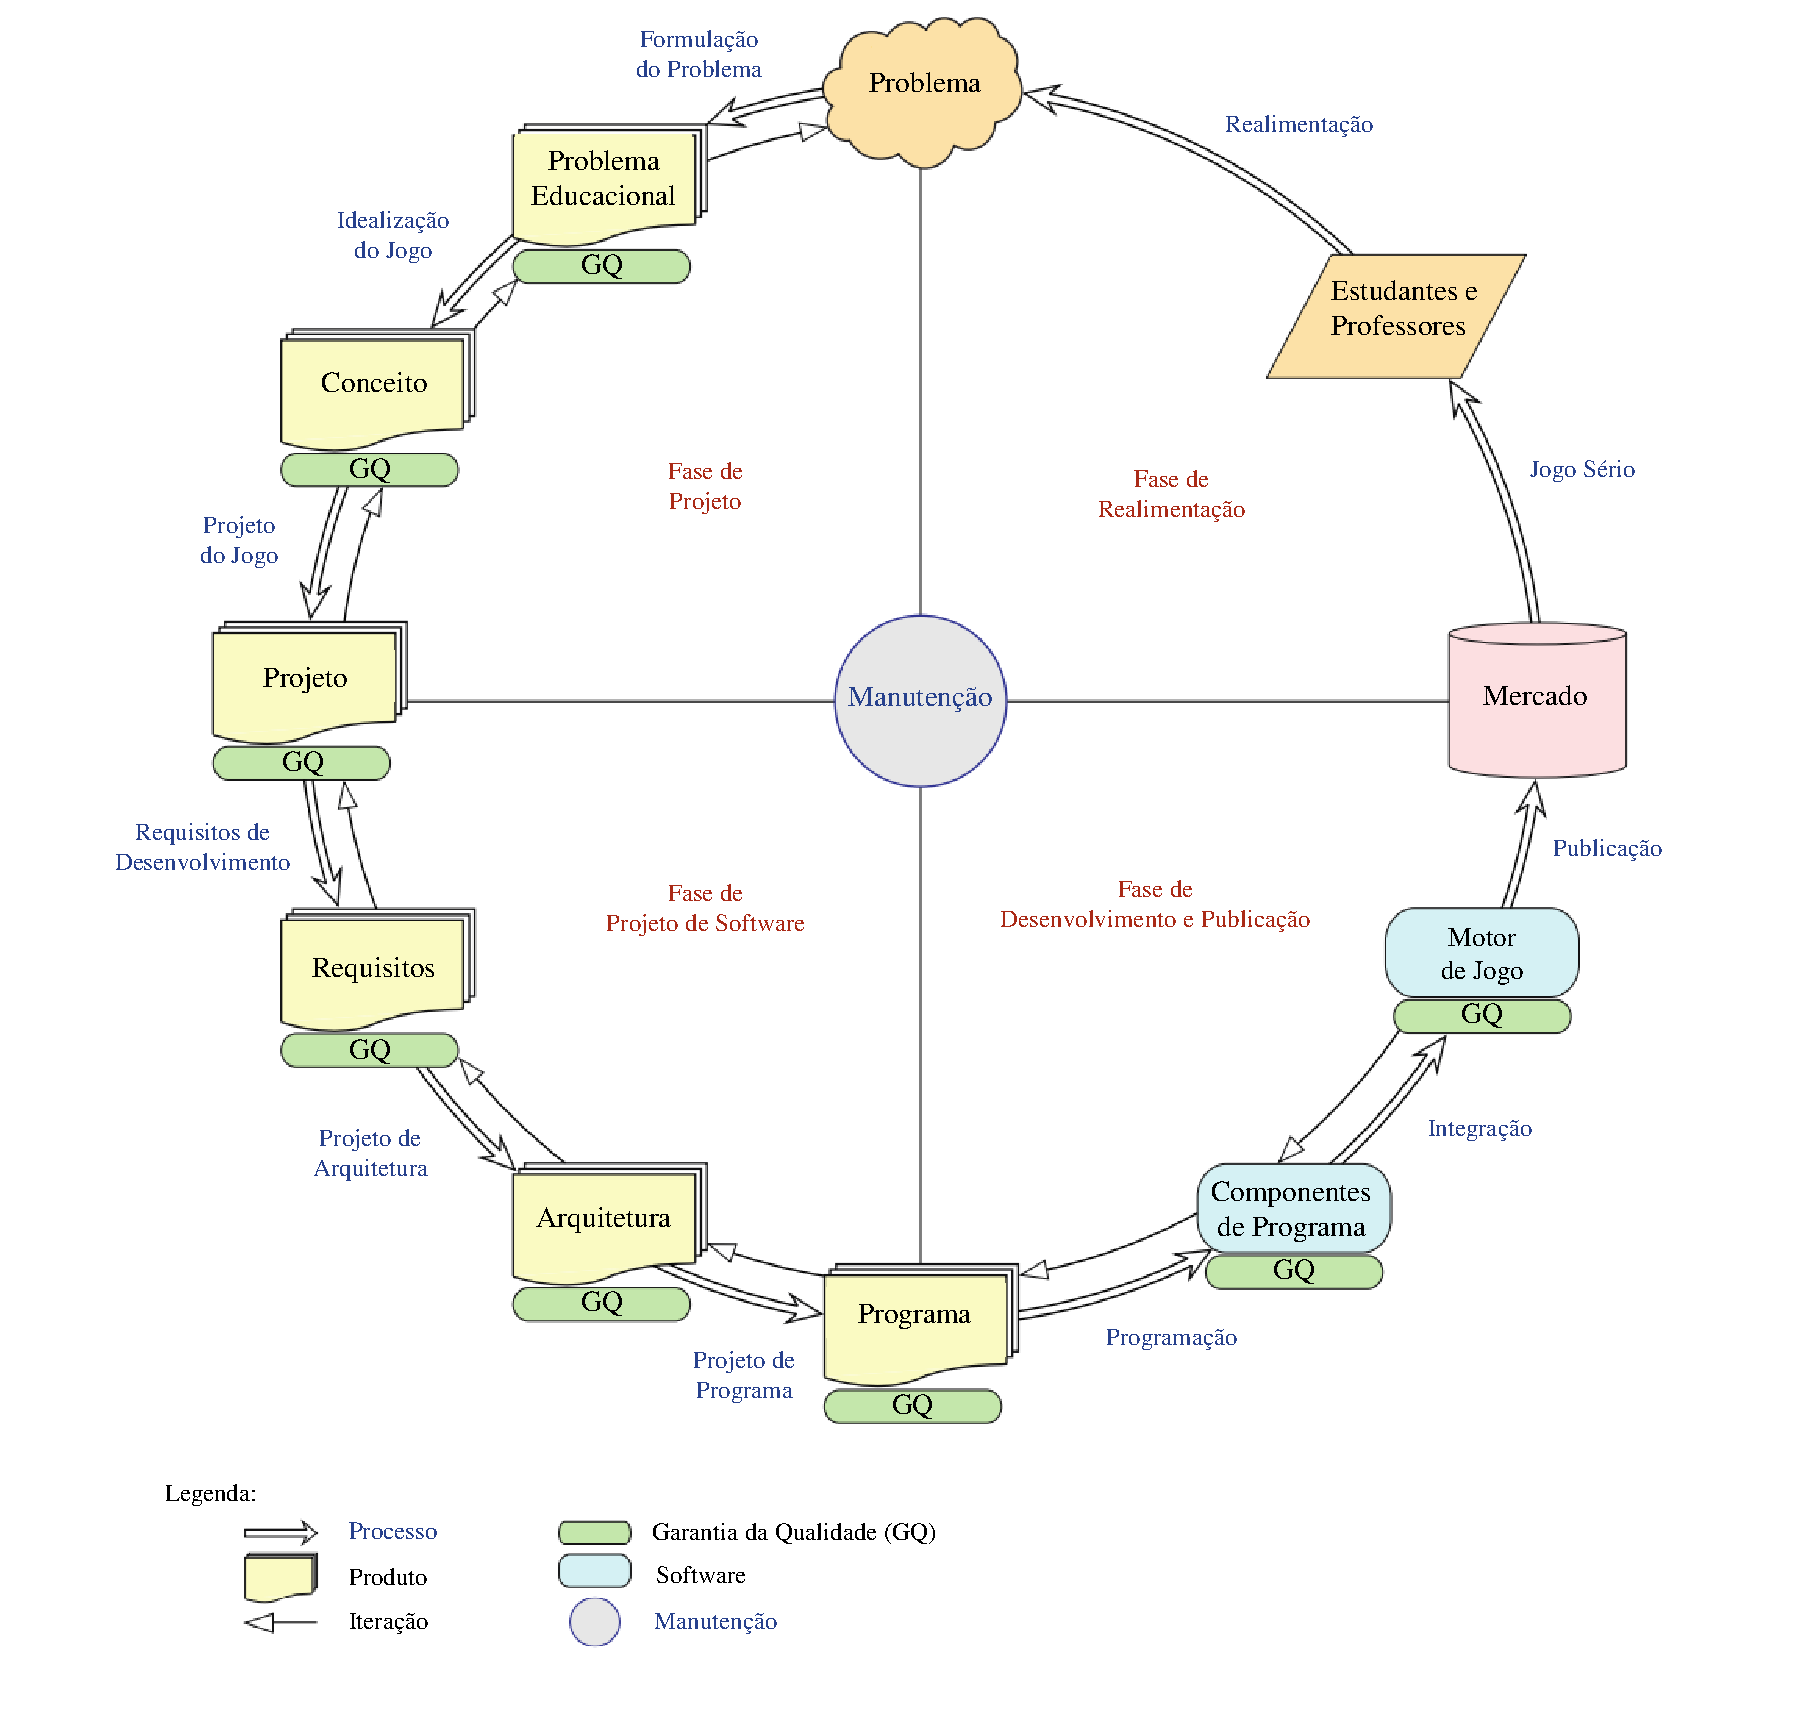
\includegraphics[width=\linewidth]{./Visuais/GAMED.pdf}}
	\end{center}%\vspace{-0.5cm}
  \legend{Fonte: adaptado de \citeonline[p. 23]{aslan2016digital}.}

\end{figure}


O ciclo da \autoref{fig:GAMED} apresenta os processos em uma forma lógica solicitante começando de um \textbf{Problema} inicial. A partir de então o ciclo se inicia na Fase de Projeto, passando pelo Projeto de \textit{Software}, pela Fase de Desenvolvimento e pela Fase de Realimentação. Ao término da última fase o ciclo se inicia novamente sendo um processo de manutenção contínuo do jogo. Cabe salientar que embora as setas mostrem um progresso sequencial, o ciclo de desenvolvimento de um jogo não precisa ser interpretado como estritamente sequencial. A representação sequencial usada na \autoref{fig:GAMED} se destina a mostrar apenas a direção do fluxo de trabalho ao longo do ciclo de desenvolvimento. 

\pagebreak

A metodologia \ac{GAMED} é iterativa tanto em sentido horário, quando em sentido anti-horário. No caso, as setas reversas almejam sanar um problema relativamente comum na área de desenvolvimento de jogos (\textit{e.g.} um determinado processo pode apontar falhas no processo anterior; para arrumar a falha é recomendado retornar ao processo anterior ao invés de esperar que o ciclo se complete por inteiro). A alternância entre os processos acontece após atingir um patamar aceitável de confiança na qualidade do jogo, por tal razão cada processo passa por uma etapa de \textbf{\ac{GQ}}. A qualidade só é atingida após um grupo qualificado confirmar que os seguintes conceitos estão devidamente empregados no jogo desenvolvido: Aceitabilidade, Desafio, Clareza, Eficácia, Engajamento, Diversão, Interatividade, Flexibilidade/Escalabilidade, Ludificação, Simplicidade, Aprendizagem e Usabilidade. 

A primeira fase do \ac{GAMED} (\textbf{Fase de Projeto}) estabelece a definição de um problema no domínio educacional para ser abordado por meio da dinâmica de jogos. O atual trabalho se objetiva a fortalecer as estratégias de enfretamento ao problema da violência sexual infantil. Por tal razão, foi realizada uma formulação do problema, identificando suas causas e consequências, além da criação conceitual do jogo. Na segunda fase do \ac{GAMED} (\textbf{Fase de Projeto de Software}); referente ao jogo produzido por este trabalho; foram catalogados os requisitos necessários para o desenvolvimento do jogo, além da escolha da arquitetura a ser utilizada. Um documento de requisitos é produzido nesta etapa. A terceira fase do \ac{GAMED} (\textbf{Fase de Desenvolvimento/Publicação}), remete especificamente ao processo de criação e desenvolvimento do jogo. O jogo deve ser produzido nesta etapa de modo a sempre disponibilizar ao final uma versão jogável. A quarta fase do \ac{GAMED} (\textbf{Fase de Realimentação}), busca apresentar um jogo brevemente finalizado a estudantes ou professores. O intuito é identificar falhas ou eventuais melhorias que podem vir a serem relatadas. Nesta etapa o jogo pode ser apresentado a outros profissionais devidamente capacitados que não precisam necessariamente contemplar o público-alvo do jogo.

O \ac{GAMED} fornece um plano detalhado para o gerenciamento de projetos complexos de desenvolvimento de jogos. Sua estrutura modularizada de desenvolvimento em fases e processos facilita o desenvolvimento de jogos educacionais digitais. O \ac{GAMED} ainda é flexível se adaptando as necessidades da equipe de desenvolvimento \cite{aslan2016digital}. Como o desenvolvimento do \ac{JS} deste trabalho envolveu essencialmente uma pessoa (o próprio pesquisador) algumas etapas do \ac{GAMED} foram supridas a fim de agilizar o processo de desenvolvimento, porém sem perder sua essência primordial. 

A compreensão dos fundamentos acerca o desenvolvimento de jogos educacionais digitais é indispensável para a progressão e conclusão deste trabalho. O presente trabalho baseia-se nos conceitos pesquisados e nas definições referenciadas nessa seção para fundamentar o processo de desenvolvimento.

%-------------------------------------------------------------------------------------------------------------------

\section{Metodologia Avaliativa}\label{sec:Avaliativos}

A avaliação de jogos educativos busca medir o seu nível de sucesso no âmbito educacional. Em outras palavras, metodologias avaliativas associadas a jogos buscam identificar se um determinado jogo é capaz de alcançar com os objetivos pré-estabelecidos. A metodologia utilizada pela presente pesquisa para constatar a eficácia de um jogo como solução educacional para prevenção da violência sexual infantil é composta por 7 (sete) procedimentos. Cada procedimento é abordado separadamente em uma subseção específica. Desta forma, a \autoref{subsec:legais} aborda sobre as considerações legais da corrente pesquisa, a \autoref{subsec:segmentacao} fala sobre o processo de segmentação da amostra, a \autoref{subsec:preteste} menciona sobre a etapa de pré-teste, a \autoref{subsec:teste} fala sobre a etapa de teste, a \autoref{subsec:posteste} discorre sobre a etapa de pós-teste, a \autoref{subsec:grupo} menciona sobre o processo de apreciação, a \autoref{subsec:documentacao} trata da etapa de documentação dos achados e a \autoref{subsec:CF} dá as conclusões da presente seção. A ordem dos procedimentos apresentados, corresponde a ordem de andamento deles na presente pesquisa. 

\subsection{Considerações Legais}\label{subsec:legais}

As considerações legais englobam toda a documentação jurídica necessária para a condução de uma determinada pesquisa. Quaisquer estudos que envolvam seres humanos como instrumento de pesquisa devem ter seus procedimentos devidamente analisados. Além disso, o envolvimento de instituições ou indivíduos deve ser judicialmente formalizado. A presente pesquisa é projetada de modo a conduzir parte de seus procedimentos em escolas da rede pública do ensino fundamental. O documento que formaliza a parceria entre essa pesquisa e escolas da rede pública é a Declaração de Ciência e Concordância das Instituições Envolvidas (\autoref{chap:DIE}). 

As parcerias firmadas pela corrente pesquisa, com escolas da rede pública, ocorrerem em comum acordo com os representantes legais das instituições de ensino envolvidas e com a \ac{SED} do município de Joinville do estado de Santa Catarina. %Salienta-se que são firmadas parcerias apenas com as escolas com corpo docente disponível para a execução dos procedimentos desta pesquisa. Isso pois, os pesquisadores são incapazes de executar os procedimentos desta pesquisa nas escolas devido há restrições legais\footnote{Portaria Conjunta SES/SED Nº 476. Art. 18 Nos estabelecimentos de ensino que ofertam o Ensino Fundamental anos iniciais, os Planos de Contingência, além das medidas sanitárias gerais determinadas nos incisos dos Art. 10 a 17 desta portaria, deverão organizar as medidas específicas de prevenção e controle relacionadas ao ensino fundamental anos iniciais, a fim de combater e mitigar o contágio da COVID-19: VI. Não é permitida a implementação dos programas e projetos intersetoriais e atividades, que são desenvolvidos por profissionais que não fazem parte do corpo docente da unidade escolar.}.
Salienta-se que o cronograma do presente trabalho é devidamente deliberado com as escolas parceiras de modo a conduzir a pesquisa sem grandes prejuízos a agenda escolar das crianças. Isso pois, todos os procedimentos envolvendo a participação de crianças no presente estudo ocorre em ambiente escolar e em horário escolar (com o intuito de agilizar o andamento e a conclusão da pesquisa). Uma vez delimitadas as datas, o envolvimento das crianças no presente estudo se inicia. 

A participação de quaisquer indivíduos em pesquisa científica deve ser firmada por meio de um documento legal. A utilização de crianças como instrumento de estudo torna necessário que as crianças atestem sua anuência em participar da pesquisa. Além disso, também é preciso a autorização formal de seus representantes legais. O documento que firma a participação de crianças na corrente pesquisa é o Termo de Assentimento (\autoref{chap:TA}). Já a autorização formal dos representantes legais das crianças é firmada pelo Termo de Consentimento Livre e Esclarecido (\autoref{chap:TCLE}). Ambos os documentos devem estar devidamente assinados para que seja válida a participação de uma determinada criança no presente estudo. %Todavia, o mesmo não se faz válido para o Termo de Consentimento para Fotografias, Vídeos e Gravações (\autoref{chap:TCF}).

%O registro de informações visuais ou sonoras ajudam as pesquisas científicas que dependem da coleta deste tipo de informação. Todavia, as pesquisas que independem destes registros (como essa pesquisa), os  requisitam para trazer maior transparência e esclarecimento sobre o andamento do estudo e dos experimentos. No entanto, para que a coleta de tais informações seja feita, é preciso a autorização legal de um determinado indivíduo ou de seu representante legal. 

%A corrente pesquisa formaliza o registro de informações visuais ou sonoras no Termo de Consentimento para Fotografias (\autoref{chap:TCF}). O termo em questão não precisa estar assinado para que um determinado indivíduo participe do estudo, justamente por essa não ser uma informação necessário para se alcançar os achados teorizados. 

%http://www1.udesc.br/arquivos/id_submenu/677/resolucao_466_12_cns__ms.pdf = 5 anos





%Os acordos de participação da corrente pesquisa são firmados inteiramente em ambiente escolar. A corrente pesquisa é apresentada ao representante legal da instituição de ensino, o qual deve assinar o documento de Declaração das Instituições Envolvidas. O recurtamento das crianças ocorrerá via a própria escola da criança. Inicialmente será devidamente requisitada a anuência das crianças em participarem da pesquisa por meio do Termo de Assentimento (\autoref{chap:TA}). Para as crianças que concordarem, serão entregues os demais termos para serem apresentados aos seus pais ou responsáveis. Uma das vias de cada termo ficará em posse dos responsáveis pela criança, enquanto a outra deverá ser apresentada na escola e entregue a um dos pesquisadores. Em síntese, a coleta das autorizações será realiza em ambiente escolar por parte dos pesquisadores e em ambiente domiciliar por parte das crianças. No ambiente escolar, a pesquisa e os pesquisadores serão apresentados a uma turma escolar (selecionada para a pesquisa e fornecida pela escola). Será lido então para toda turma Termo de Assentimento da pesquisa. Após a leitura do termo será questionado a turma sobre as crianças interessadas em participar da pesquisa. Aos interessados será entregue o Termo de Assentimento impresso, conjuntamente com os termos: Termo de Consentimento Livre e Esclarecido (\autoref{chap:TCLE}); Termo de Consentimento para Fotografias (\autoref{chap:TCF}). Será requisitado que todos os termos sejam apresentados aos devidos responsáveis legais de cada crianças e assinados. Uma das vias (assinada) deverá ser levada a escola para ser colhida por um dos pesquisadores. Só participarão da pesquisa as crianças que comprovarem autorização dos pais. Visando garantir a integridade das assinaturas e fugir de falsificações cada assinatura será comparada ao documento de matrícula escolar assinado na escola presencialmente pelos pais de cada criança. Salienta-se que a não assinatura dos Termo de Consentimento para Fotografias (\autoref{chap:TCF}) não invalida a participação do menor na pesquisa em questão. Todos os procedimentos legais ocorerrão presencialmente (podendo ser por um dos pesquisadores responsáveis ou por outro responsável optado pela escola). A aplicação da pesquisa de modo presencialmente permite um acompanhamento mais zeloso as crianças, garantido a fiscalização e o monitoramento dos participantes a fim de evitar ao máximo quaisquer danos. Com o término da coleta de documentação legal (prevista para ser concluida em até um mês), a presente pesquisa é capaz de prosseguir para os demais procedimentos.


\subsection{Segmentação}\label{subsec:segmentacao}

Em pesquisa científica, o processo de segmentação está associado, em grande parte, ao isolamento de variáveis. Academicamente, almeja-se isolar variáveis para se compreender melhor os resultados de uma determinada pesquisa. No caso das pesquisas envolvendo seres humanos, o processo de segmentação, normalmente diz respeito a segregação de uma amostra de indivíduos. Para essa pesquisa, o processo de segmentação se deu com base nas turmas escolares das crianças de forma totalmente aleatória. Ou seja, as crianças válidas em participar da presente pesquisa são separadas em dois grupos distintos com base em suas turmas, onde crianças da mesma turma, acabam por pertencer ao mesmo grupo. Os dois grupos que definem o presente estudo são: grupo controle e grupo experimental. 

O grupo controle representa o grupo de indivíduos que não são submetidos a um objeto estudado, servindo como uma variável controle. Já o grupo experimental é o grupo de indivíduos que são submetidos a um objeto estudado. No caso da atual pesquisa o objeto estudado é um jogo educacional para prevenção da violência sexual infantil. Por se tratar de um processo aleatório, é impossível que um determinado indivíduo saiba a qual grupo pertencerá, antes que a etapa de segmentação esteja concluída. A conclusão da presente etapa inicia a etapa de pré-teste. 

%discorrer sobre a separação em grupos da amostra. Em pesquisas experimentais o processo de segementação de uma amostra de indivíduos deve obedecer uma distribuição aleatória. Para essa pesquisa a divisão entre os grupos controle e experimental ocorrerá em turmas escolares (visando agilizar o processo). Isso pois, acredita-se que as turmas de uma escola já são montadas de forma aleatória. Salienta-se que no corrente momento não se sabe da quantidade de crianças que participarão da pesquisa, por tal razão não se sabe quantos grupos controle e experimental existirão, devendo haver no mínimo um grupo de cada com 30 crianças ao menos para essa pesquisa ser encontradas nos requisitos mínimos do rigor científico.

%Nos termos nos quais as assinaturas foram requisitadas (\autoref{chap:TCLE}, \autoref{chap:TA}) não constam o grupo determinado que a criança poderá cair, no entando, todos os procedimentos tomados com cada grupo são descritos. A divisão não ocorrerá de forma presencial. O tempo previsão para essa etapa é de um dia, ao término dessa etapa a presente pesquisa pode adentrar na etapa de pré-teste. 

\subsection{Pré-teste}\label{subsec:preteste}

Na academia científica, a etapa de pré-teste é utilizada normalmente com o intuito de se mensurar uma variável ou um conjunto de variáveis. O objetivo da etapa de pré-teste é justamente coletar informações antes que um determinado experimento ocorra, permitindo assim, uma comparação mais clara, entre os resultados alcançados antes de um teste e os resultados alcançados depois deste mesmo teste. Na área da avaliação cognitiva, a coleta de informações tende a ser realizada por meio de um instrumento avaliativo. No caso, a presente pesquisa tem como foco medir os níveis de conhecimento sobre a prevenção da violência sexual. O modelo avaliativo, mais presente na literatura pesquisada, para se medir os níveis de conhecimento sobre a prevenção da violência sexual é o \ac{CKAQ}.

O \ac{CKAQ} é um instrumento avaliativo desenvolvido para avaliar o nível de conhecimento sobre a prevenção do abuso \cite{tutty1992ability}. O \ac{CKAQ} é direcionado para crianças entre 5 (cinco) e 12 (doze) anos de idade, sendo constituído por 33 (trinta e três) questões de múltipla escolha. O tempo de finalização para o \ac{CKAQ} é de 15 (quinze) minutos. O instrumento avaliativo em questão apresenta largo uso nas pesquisas e demonstra-se apropriado ao avaliar a aprendizagem sobre conceitos básicos de prevenção incluídos em programas educacionais de prevenção ao abuso sexual de crianças \cite{tutty1992ability}. O presente trabalho adapta para o português (\refanexo{chap:traduzido}), com auxílio da psicóloga Letícia Schneider Tidra, o \ac{CKAQ} original (\autoref{chap:CKAQ}). A versão adaptada é utilizada pelo presente trabalho para validar o programa educacional proposto pela atual pesquisa. O processo de validação é melhor descrito na \autoref{ch:Avaliacao}.

%O questionário em questão possui algumas versões que foram produzidas ao longo dos anos \cite{tutty1995revised, tutty2019children}. No geral as versões variam apenas em números de questões, existindo versões do questionário com apenas dez questões, construídas com o intuito de auxiliar o pesquisador e agilizar os experimentos. Os questionários resumidos apresentam um grau de confiança aceitável para pesquisas, contudo são aconselháveis apenas para as situações nas quais a medição dos conhecimentos sobre a prevenção da violência infantil não sejam o foco da pesquisa. 


\subsection{Teste}\label{subsec:teste}

No âmbito científico, a etapa de teste está associada à ações ou perturbações realizadas por uma determinada pesquisa. No caso, a presente pesquisa realiza intervenções com um jogo educacional, com o intuito de atestar sua eficácia no ensino didático de crianças, no que diz respeito a prevenção da violência sexual infantil. A depender da disponibilidade e da vontade da escola parceira desta pesquisa, o jogo em questão é ministrado via: computador, \textit{smartphone} ou \textit{tablet}. A administração do jogo para as crianças é realizada de maneira individual, ou seja, uma criança por dispositivo, com as crianças compartilhando o mesmo ambiente. Todas as questões pedagógicas abordadas pelo jogo são descritas em maiores detalhes no \autoref{ch:Desenvolvimento}. 

O jogo desenvolvido pelo presente trabalho possui 4 (quatro) fases relacionadas de alguma forma a prevenção da violência sexual infantil. Os assuntos trabalhos por cada uma das fases são: Anatomia, Direitos, Denúncias e Redes Sociais. Cada fase do jogo é jogada pelas crianças do grupo experimental, apenas. As crianças são convidadas a jogar o jogo de acordo com a agenda de cada escola parceira, salientando que não existem ordem previamente estabelecida para a conclusão das fases. Durante a etapa de teste, a performance das crianças no jogo é colhida. Em outras palavras, informações sobre os seus acertos, erros e tempos de respostas no jogo são enviados a um banco de dados para análise futura. O último dia de teste demarca o início da etapa de pós-teste. 

%FORAM COLETADOS OS DESEMPENHOS OS GRUPOS VIA REDE, OS ACERTO E ERROS ERAM ANEXADO EM UM BANCO DE DADOS RELACIONAL A FIM DE COMPARAR COM OS RESULTADOS DOS TESTES (NO CASO DO GRUPO EXPERIMENTAL). ASSIM, É POSSIVEL OBSERVAR UMA POSSIVEL RELAÇÃO ENTRE O DESEMENHO NO JOGO E NAS APRENDIZAGEM ADQUIRIDAS PELO JOGADOR (OU NÃO).

%Os experimentos com o jogo podem ser realizados em uma sala de aula ou em uma sala de informática (ou outro ambiente optado pela escola). Para os não participantes, as crianças serão deslocadas para outro ambiente da escola, a depender dos responsáveis da instituição, podem ser enviadas palavra um biblioteca escolar, ginásio, ou outro cômodo escolar. A responsabilidade e o cuidado destas crianças é de responsabilidade da escola.

\subsection{Pós-teste}\label{subsec:posteste}

A etapa de pós-teste vem de modo a completar a etapa de pré-teste. O objetivo da etapa de pós-teste é justamente coletar informações após a ocorrência de um determinado experimento, permitindo assim, uma comparação mais clara, entre os resultados alcançados antes de um teste e os resultados alcançados depois deste mesmo teste. Deste modo, os procedimentos conduzidos na etapa de pós-teste de uma pesquisa científica, tendem a seguir os mesmos procedimentos já conduzidos na etapa de pré-teste. 

A atual pesquisa busca identificar discrepância cognitivas entre o grupo controle e o grupo experimental no que diz respeito aos seus conhecimentos sobre a prevenção da violência sexual infantil (Teste-t). Para tal, o instrumento avaliativo \ac{CKAQ} é aplicado a amostra de participantes da presente pesquisa. Salienta-se que a presente pesquisa não exige que os participantes do grupo experimental tenham completado a etapa de teste para participar da etapa de pós-teste. Em outras palavras, todo o processo de aplicação do instrumento avaliativo descrito na etapa de pré-teste da presente pesquisa, se faz válido para a etapa de pós-teste. No mais, a presente pesquisa não se dispõem a calcular a consistência interna do questionário e nem a julgar a eficácia do questionário em si. A presente pesquisa se dispõem apenas a coletar as respostas das crianças participantes e comparar os resultados absolutos de seus grupos com auxílio do Teste-t. A finalização da presente etapa inicia a etapa de apreciação.

%A compreensão dos fundamentos para a validação de jogos educacionais é indispensável para a progressão e conclusão deste trabalho. O presente trabalho baseia-se nos conceitos pesquisados e nas definições referenciadas nessa seção para fundamentar e guiar o processo de validação do jogo desenvolvido por esta pesquisa. A validação e submissão do questionário ocorre em dois momentos distintos da pesquisa, na etapa de pré-teste e pós-teste. O processo avaliativo é constituído por dois grupos, um grupo experimental e um grupo controle sem quaisquer diferenças étnicas ou socio-econômicas aparentes entre os grupos (e dentro dos grupos). Para a comparação dos resultados entre os grupos se utilizará o Teste-t. 


\subsection{Apreciação}\label{subsec:grupo}

A apreciação tende a estar associada as pesquisas de satisfação. O principal intuito é identificar os níveis de satisfação de um indivíduo ou grupo de indivíduos acerca um determinado produto ou serviço. A presente pesquisa realiza sua etapa de apreciação apenas com as crianças do grupo experimental. O processo em si consiste em verificar os níveis de engajamento e agradabilidade do jogo desenvolvido pela presente pesquisa.  (\refanexo{chap:MEEGA})  (\autoref{chap:Apreciacao})

A etapa de apreciação da presente pesquisa faz uso do \ac{MEEGA} \cite{savi2011avaliacao}. O \ac{MEEGA} é um modelo que avalia jogos educacionais em termos de motivação, experiência do usuário e aprendizagem por meio da reação dos estudantes \cite{petri2019meega+}. A escala para avaliação de jogos educacionais possui 27 itens padronizados e um conjunto de itens customizados para os objetivos de aprendizagem de cada jogo. o modelo foi adapatdo (versão original Anexo) nova versão (Apêndice).

A etapa de apreciação da presente pesquisa convida seus participantes a se manifestarem livremente sobre sua experiência no jogo. Todas as críticas e elogios são devidamente catalogados para análise futura. A etapa de apreciação é realizada em uma turma escolar, onde é dado vez a todos os participantes da pesquisa em manifestarem seus pensamentos e sugestões sobre o jogo. A duração desta etapa é de uma hora. A conclusão desta etapa encerra a participação de terceiros nesta pesquisa, dando início a etapa de documentação. 

%A apreciação busca identificar os níveis de agradabilidade de um indivíduo ou um grupo com um determinado produto. No caso a presente pesquisa o Engajamento (dado qualitativo) será colhido por meio de entrevistas realizadas presencialmente e em grupo com a amostra de crianças que jogou o jogo (grupo experimental), as crianças serão convidadas a se manifestarem livremente sobre sua experiência no jogo, esse processo busca identificar possíveis desconfortos que o jogo possa ter causando em algum momento. Além disso, será requisitado para todas as crianças darem uma nota ao jogo.

\subsection{Documentação}\label{subsec:documentacao}

A etapa de documentação consiste em reportar os principais achados de um determinado experimento científico. No caso da presente pesquisa, todos os seus procedimentos, resultados e achados são devidamente documentados e publicados sem a identificação das crianças envolvidas. A documentação dos achados e resultados desta pesquisa é realizada no \autoref{ch:Conclusao}. Salienta-se que todos os participantes desta pesquisa são informados sobre o local de publicação desta pesquisa científica. 

%Salienta-se que não cabe a essa pesquisa a tarefa de informar a todos os participantes envolvidos, o local e a data de publicação dos resultados do presente estudo. 

O processo de documentação é crucial para o fortalecimento e enriquecimento do corpo científico. A etapa de documentação permite a dispersão dos conhecimentos alcançados por um estudo; possibilitando assim, que seus resultados possam ser averiguados por futuras pesquisas, as quais podem confirmar ou até mesmo refutar seus achados. Visando atingir uma maior dispersão do conhecimento, a presente pesquisa realiza a publicação de seus achados de forma totalmente gratuita e de livre acesso.

\newpage

\subsection{Considerações Finais}\label{subsec:CF}

Os procedimentos descritos nessa seção buscam trazer maior esclarecimento sobre o andamento desta pesquisa. Salienta-se nesse sentido que o intervalo padrão entre a maioria dos procedimentos descritos é de um mês, variando alguns dias, a depender da agenda escolar de cada instituição de ensino parceira. O procedimento de apreciação é a única exceção, ocorrendo imediatamente após o término do procedimento de pós-teste. Para os procedimentos envolvendo contato direto com as crianças os protocolos sanitários de cada instituição de ensino parceira são devidamente respeitados. Deste modo, enfatiza-se que todos os procedimentos envolvendo crianças são realizados inteiramente em ambiente e em horário escolar, com o objetivo de evitar ao máximo a circulação e o deslocamento das crianças. A depender da escola, os procedimentos são realizados em salas de informática ou até mesmo nas próprias salas de aula tradicionais. 

%O intervalo de tempo entre os procedimentos fica na casa de um mês, podendo variar um pouco a depender da agenda escolar de cada instituição de ensino. Além disso, todos os procedimentos hão de obedecer os protocolos sanitários de cada instituição. Os procedimentos serão realizados todos em ambiente escolar, visando ao máximo evitar a circulação e deslocamento das crianças. A depender da escola, os procedimentos podem ser realizados em salas de informática ou até mesmo nas próprias salas de aula tradicionais. 

Só são válidas em participar desta pesquisa as crianças falantes do português entre 5 (cinco) e 8 (oito) anos de idade com a devida autorização de seus guardiões. São dispensadas em participar desta pesquisa as crianças que não contemple esses critérios ou crianças incapazes de realizar as etapas necessárias para a execução desta pesquisa (por qualquer razão). Para as crianças válidas em participar desta pesquisa, informa-se que todos os riscos do presente estudo são mínimos aos participantes. No caso do jogo em si, salienta-se do risco de crianças fotossensíveis manifestarem enjoos ou tonturas durante os experimentos. No caso da temática envolvida, enfatiza-se dá possibilidade dos assuntos apresentados trazerem desconfortos ou incômodos aos participantes. Visando minimizar esses riscos, a presente pesquisa informa que todos os participantes que apresentarem o primeiro sinal de risco são afastados da pesquisa e encaminhados para sua agenda escolar tradicional, o processo de afastamento é devidamente comunicado ao Comitê de Ética. Enfatiza-se que é de inteira responsabilidade da instituição de ensino parceira os cuidados a serem tomados para com os não-participantes desta pesquisa. 

%Informa-se que só poderão participar dessa pesquisa as crianças que passarem pelos devidos tramites legais de autorização. Os riscos de todos os procedimentos serão mínimos para os participantes. No caso do jogo em si, salienta-se do risco de crianças fotossensíveis manifestarem enjoos ou tonturas durante os experimentos. No caso da temática envolvida, enfatiza-se dá possibilidade dos assuntos apresentados trazerem desconfortos ou incômodos aos participantes. Visando minimizar esses riscos, a presente pesquisa informa que todos os os participantes que apresentarem o primeiro sinal de risco serão afastados da pesquisa e encaminhados para sua agenda escolar tradicional, o processo de afastamento será devidamente comunicado ao Comitê de Ética. Crianças que não contemplem o pública alvo do jogo também já serão previamente desclassificadas.

As crianças não aptas a participar desta pesquisa, presentes em uma turma de crianças aptas, são devidamente encaminhadas a outras atividades escolares sem prejuízo aos protocolos educacionais vigentes\footnote{Art. 18 Nos estabelecimentos de ensino que ofertam o Ensino Fundamental anos iniciais, os Planos de Contingência, além das medidas sanitárias gerais determinadas nos incisos dos Art. 10 a 17 desta portaria, deverão organizar as medidas específicas de prevenção e controle relacionadas ao ensino fundamental anos iniciais, a fim de combater e mitigar o contágio da COVID-19: III. Os alunos de cada turma devem ficar sempre na mesma sala, para evitar troca de espaços e maior movimentação nos corredores.}. Ao término dos experimentos, a turma escolar inteira retorna a sua agenda escolar tradicional. A participação no atual estudo científico não envolve gastos aos participantes. Também, não a qualquer punição jurídica ou financeira para qualquer participante que abandone a presente pesquisa. Como frutos dessa pesquisa informa-se que haverá o benefício indireto por parte de todos os participantes em ajudarem a ampliar o rigor do processo científico. Espera-se que os participantes do grupo experimental se beneficiem ao desenvolver habilidades que os permitam a reconhecerem, evitarem e relataram episódios praticados (ou tentados) de violência sexual. No casos particulares de relatos de violência sexual infantil manifestados durante a pesquisa, a presente pesquisa espera que a criança seja beneficiada ao ter uma vida mais digna. Isso pois, estes casos hão de ser devidamente denunciado como determina a Lei Federal nº 8.069, de 13 de julho de 1990 (\ac{ECA}) e a Resolução nº 4666674 de Joinville (Protocolo de Atendimento às pessoas em situação de violência sexual do município de Joinville/SC). 

%Os resultados alcançados com o grupo estudado se demonstrar bem sólidos e robustos. Isso pois, a presente pesquisa se utiliza do Teste-t com um grau de confiança de 95\%. A alta taxa de confiança estatística do presente estudo, abre margem para uma defesa sólida e robusta de seus resultados. 

No que diz respeito a amostra de participantes, a presente pesquisa enfatiza que não são coletadas informações étnicas, socioeconômicas ou religiosas. A presente pesquisa só se dispõe a coletar informações relacionadas a idade e ao desempenho cognitivo de sua amostra de participantes. A condição financeira ou social dos envolvidos não são analisadas e nem julgadas, portanto, não há o que afirmar sobre a influência destas variáveis na correte pesquisa. Logo, os resultados e achados desta pesquisa se demonstram válidos apenas para o grupo estudado, nada se pode afirmar sobre a estrapolação dos resultados desta pesquisa para a população em geral. 

%Os benefícios e vantagens em participar deste estudo estão relacionados com o fortalecimento do processo científico, além da evolução científica dos arcabouços projetados. Caso os pressupostos teóricos estejam corretos, espera-se que os participantes do grupo selecionado se beneficiem ao desenvolver habilidades que os permitam a reconhecerem, evitarem e relataram episódios praticados (ou tentados) de violência sexual, ampliando assim a segurança pessoal das crianças do grupo selecionado que jogaram o arcabouço desenvolvido. 

%Salienta-se que nenhum dos participantes terão gastos em participar dessa pesquisa e nem serão punidos caso optem em abandonar a pesquisa. Contudo, como frutos dessa pesquisa informa-se que haverá o benefício indireto por parte de todos os participantes em ajudarem a aplicar o rigor do processo científico. Para os participantes do grupo experimental, espera-se que os participantes do grupo selecionado se beneficiem ao desenvolver habilidades que os permitam a reconhecerem, evitarem e relataram episódios praticados (ou tentados) de violência sexual, ampliando assim a segurança pessoal das crianças do grupo selecionado que jogaram o arcabouço desenvolvido.

%Os resultados e achados desta pesquisa não são válidos para toda a população em geral. Todas as descobertos envolvendo o desenvolvimento de habilidades preventivas a violência sexual por meio de um jogo educativo são válidas apenas para o grupo testado. As crianças participantes da atual pesquisa não possuem grandes diferenças étnicas ou socio-econômicas. Desta forma, os resultados e achados do atual estudo podem não valer para toda a população em geral. É preciso que pesquisa futuras sejam conduzidas de modo a abrager um amostra de participantes com maior variabilidade, podendo assim, extrapolar seus resultados para a população geral. Todavia, os resultados alcançados com o grupo estudado se demonstrar bem sólidos e robustos. Isso pois, a presente pesquisa se utiliza do Teste-t com um grau de confiança de 95\%. A alta taxa de confiança estatística do presente estudo, abre margem para para uma defesa sólida e robusta de seus resultados. 

A participação e envolvimento de crianças no presente estudo, ocorre, em grande parte, de forma presencial e de maneira coletiva (em uma turma escolar). A aplicação da pesquisa de modo presencialmente permite um acompanhamento mais zeloso as crianças, garantido a fiscalização e o monitoramento dos participantes a fim de evitar ao máximo quaisquer danos. Já aplicação da pesquisa de modo coletivo, possibilita que os procedimentos possam ser conduzidos de maneira mais rápida e ágil. O acompanhamento e a condução dos procedimentos da presente pesquisa envolvendo de maneira direta as crianças participantes é conduzido por um indivíduo optado pela instituição de ensino parceira (membro do corpo docente da unidade escolar). Os procedimentos que não depende da participação direta de terceiros (\textit{e.g.} segmentação e documentação) são conduzidos pelo autor desta dissertação. Toda informação gerada pela presente pesquisa é armazenada conforme ordena\footnote{A resolução nº 510, de 7 de abril de 2016, obriga o pesquisador manter os dados de sua pesquisa em arquivo, físico ou digital, sob sua guarda e responsabilidade, por um período mínimo de 5 (cinco) anos após o término de sua pesquisa.} o \ac{CNS}. A documentação formal da presente pesquisa encerra seu envolvimento no corpo científico.



%E necessidade de um grupo controle vem de modo a isolar a variavel do crescimento infantil.




\chapter{Estratégias de Combate ao Problema}\label{ch:Relacionados}

O \acf{ASI} manifesta-se como um problema global. Diante disso, profissionais da saúde e pesquisadores passaram a se dedicar a compreender as raízes  deste mal que assola milhares de crianças todos os anos \cite{deslandes1994atenccao, dahlberg2006violencia, hora2017violencia}. A área de criminologia em específico, desenvolveu uma série de teorias acerca das causas para os atos infracionais. Dentre elas, destaca-se a Teoria da Atividade Rotineira, ilustrada na \autoref{fig:Crime}.

\begin{wrapfigure}{r}{8.0cm}
  \vspace{-0.6cm}\caption{\label{fig:Crime}Triângulo do Crime.}
        \begin{center}
          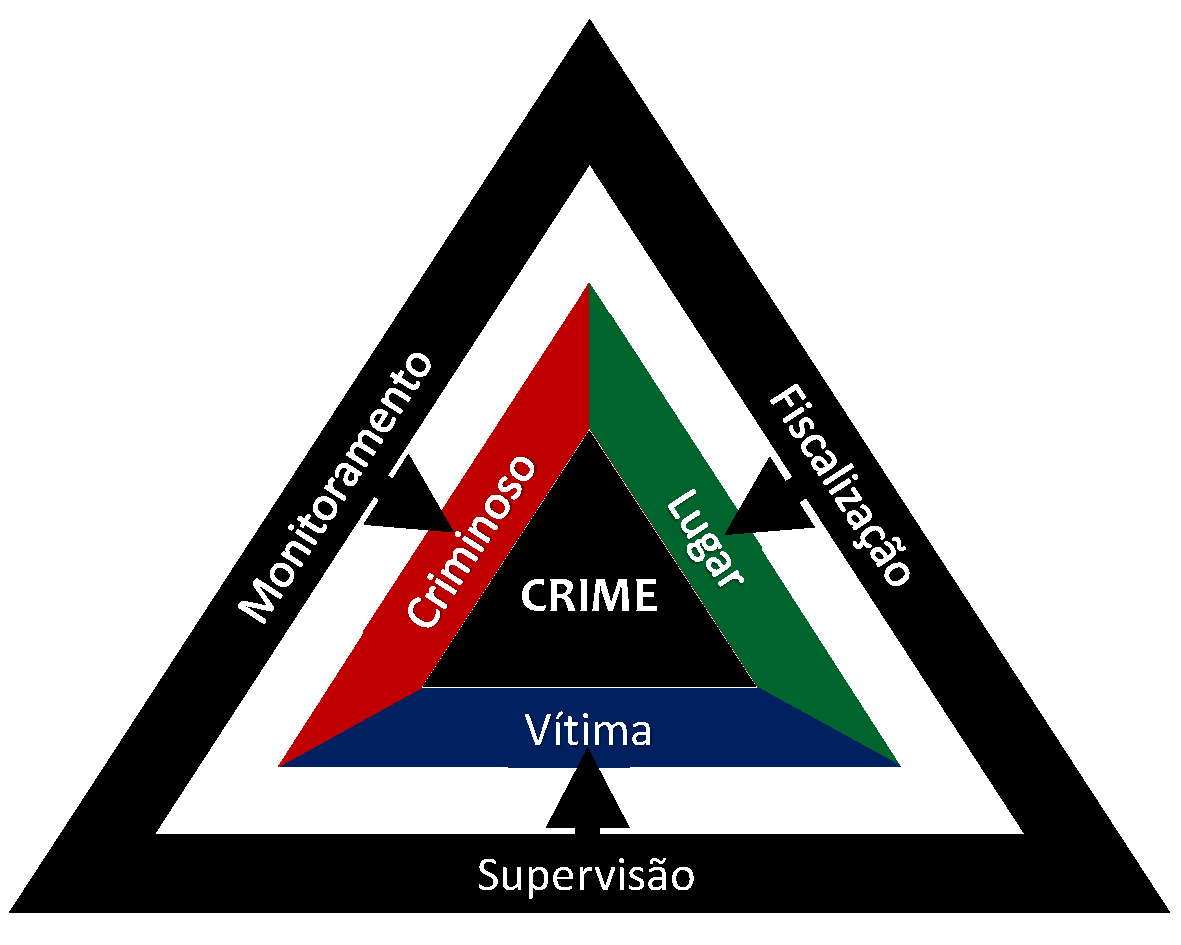
\includegraphics[width=\linewidth]{./Visuais/TrianguloCrime.pdf}
        \end{center}
        \legend{Fonte: Elaborada pelo autor (2020).}
\end{wrapfigure}

O infográfico da \autoref{fig:Crime} apresenta os três elementos básicos da Teoria da Atividade Rotineira, também conhecida como Triângulo do Crime. Em resumo, três elementos são considerados essenciais para a ocorrência de um crime. Para que um crime aconteça deve-se haver um criminoso motivado sem supervisão, um lugar sem fiscalização e uma vítima desprotegida ou vulnerável. Tomar atitudes preventivas sob qualquer um destes elementos, dificulta a ocorrência do crime. Todavia, destaca-se que estes elementos não possuem pesos iguais, mas sim, se interbalanceiam entre si (\textit{e.g.} em certas condições, um lugar bem fiscalizado poderia não ser um empecilho para um criminoso muito motivado).

O Triângulo do Crime apresenta as três partes fundamentais para a ocorrência de um crime. As estratégias de combate ao \ac{ASI} se objetivam a agir sob estas partes fundamentais. Algumas estratégias são focadas no monitoramento de criminosos\footnote{\label{note:nota1}O Canadá conduz um programa comunitário de acompanhamento de infratores sexuais denominado \textit{Circles of Accountability and Support} (CoSA). O programa se objetiva a ajudar e a apoiar agressores sexuais à se reintegrarem à sociedade após cumprirem suas penas de encarceramento. Estudos mostram que o programa é capaz de reduzir em até 80\% a reincidência do crime entre os participantes \cite{wilson2009circles}. Mais informações sobre o programa canadense podem ser acessadas em: \url{https://www.cosacanada.com/}.}, outras no fortalecimento da fiscalização de espaços públicos ou privados\footnote{No Brasil, a lei nº 12.038 visa dificultar a exploração sexual de crianças e adolescentes, ampliando medidas punitivas para os estabelecimentos que hospedarem menores desacompanhados dos pais ou responsáveis, ou sem autorização. Disponível em: \url{http://www.planalto.gov.br/ccivil_03/_Ato2007-2010/2009/Lei/L12038.htm}.}, e outras na capacitação preventiva de potenciais vítimas, tornando-as menos vulneráveis\footnote{A iniciativa educacional \textit{Child Abuse Prevention Program} (CAPP) busca ensinar crianças à reconhecer, resistir e denunciar abusos. Mais informações sobre o programa podem ser acessadas em: \url{https://www.nyfoundling.org/what-we-do/our-programs/child-welfare/child-abuse-prevention-program-capp/}.}. Cada estratégia pode ser dividida com base em seus níveis de prevenção, podendo ser: prevenção primária, prevenção secundária ou prevenção terciária. Os níveis de prevenção são apresentados em maiores detalhes na \autoref{fig:prevencao}.


\begin{figure}[htb]
	\caption{\label{fig:prevencao}Níveis de Prevenção.}
    \vspace{0.4cm}
    \hspace{-0.75cm}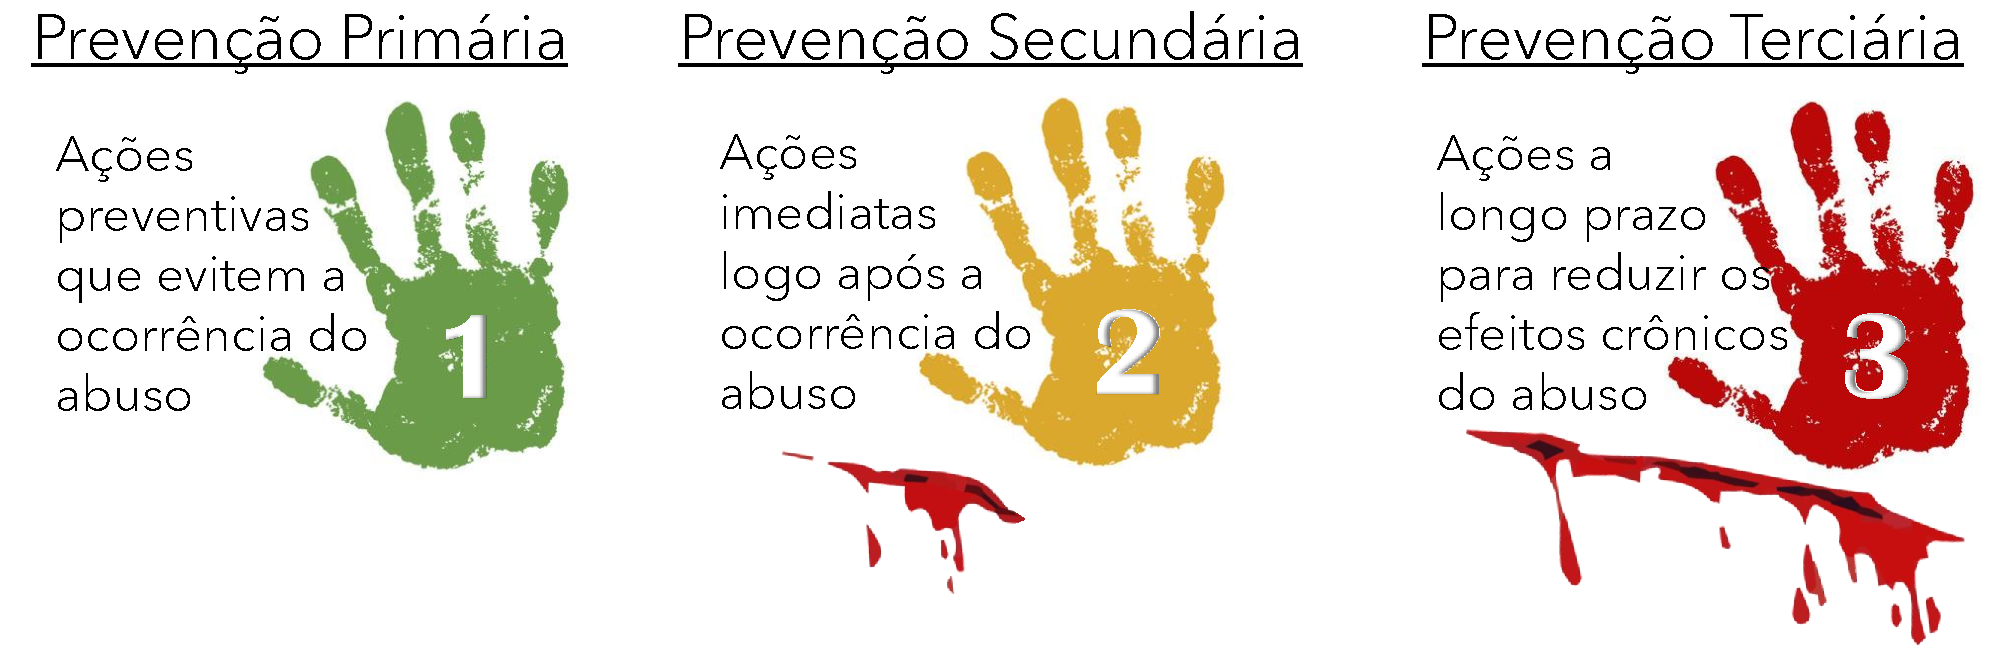
\includegraphics[width=1.1\linewidth]{./Visuais/Prevencao.pdf}

	\legend{Fonte: Elaborada pelo autor (2020).}
\end{figure}

A \autoref{fig:prevencao} apresenta os três níveis de prevenção mais comumente relatados na literatura pesquisada. São eles: prevenção primária, prevenção secundária e prevenção terciária \cite{dahlberg2006violencia, santos2011guia, maria2012abusos, cardoso2015abuso}. No caso do \ac{ASI}, a prevenção primária engloba iniciativas que antecipam a incidência do abuso sexual contra crianças e adolescentes  \cite{marcelino2017vamos}. A prevenção secundária enfatiza uma resposta imediata após a ocorrência da violência sexual. Já a prevenção terciária corresponde, de modo geral, a ações de longo prazo para o tratamento e recuperação das vítimas \cite{escocia2020expert}. Informa-se que a literatura médica relata também um quarto nível de prevenção. A prevenção quaternária descreve sobre ações preventivas contra eventuais exageros na utilização de métodos preventivos \cite{tesser2017importante}. Embora presente na literatura médica, salienta-se que a atual dissertação engloba apenas os três níveis de prevenção mais relatados pela bibliografia pesquisada acerca do abuso sexual de crianças e adolescentes.

Os níveis de prevenção do \ac{ASI} não se resumem a atuar apenas sob as crianças. Há registros de prevenção terciária relacionados inclusive ao tratamento/acompanhamento de agressores sexuais\footref{note:nota1}. O combate ao abuso sexual de crianças e adolescentes assume então inúmeras facetas, cada qual, objetivada a diminuir de alguma forma os fatores de risco que influenciam a ocorrência de violações sexuais.

Os \ac{FRs} são aquelas circunstâncias que aumentam a probabilidade da ocorrência de um episódio de violência. Deste modo, o abuso infantil apresenta mais chances de ocorrer quando os fatores de risco se acumulam. Os \ac{FRs} interagem entre si, no que é chamado de risco em cascata, no qual um risco inicial pode acompanhar ou desencadear outros riscos, terminando por resultar em um acúmulo sucessivo de fatores de risco \cite{Recommendations2019Taylor}. A \autoref{fig:Riscos} apresenta a disposição dos fatores de riscos mais apontados pela literatura na área por meio de um Modelo Ecológico. 

\pagebreak

\begin{figure}[htb]

    \caption{\label{fig:Riscos}Modelo Ecológico para a compreensão da violência contra crianças.}
    \hspace{-2.8cm}
    %\begin{center}
      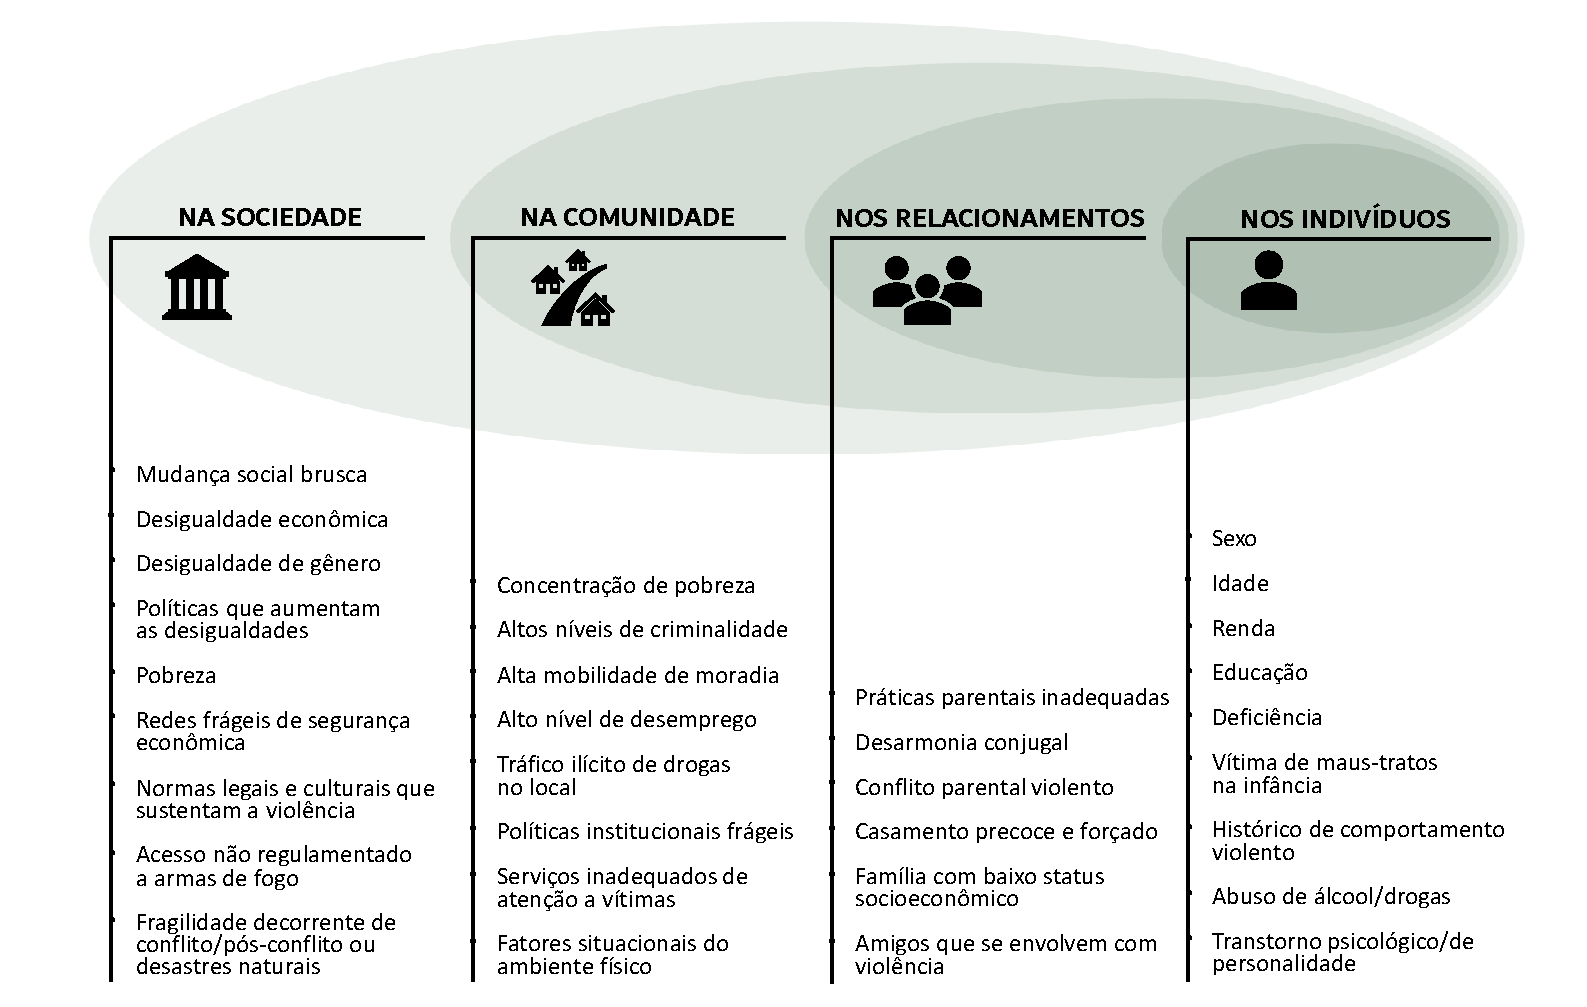
\includegraphics[width=1.28\linewidth]{./Visuais/Ecologico.pdf}
      %\end{center}
    \legend{Fonte: adaptado de \citeonline[p. 17]{inspire2016seven}.}
  
  \end{figure}

O Modelo Ecológico da \autoref{fig:Riscos} ilustra os quatro fatores de risco mais presentes na bibliografia pesquisa. Salienta-se que os fatores de risco podem variar em quantidade e em nomenclatura, dependendo da fonte literária \cite{centers2004sexual, sexual2017department, blasco2018abuso, UNICEF2016promising}. Todavia, a ideia base do Modelo Ecológico tende a permanecer inalterada. O modelo em si, explora a relação entre os fatores individuais e contextuais que acabam por implicar em um cenário de violência \cite{dahlberg2006violencia}. Os fatores de risco do abuso sexual de crianças e adolescentes mais influentes são:

\begin{itemize}
    \item \textbf{Individual:} \hfill Aspectos individuais que fomentem a ocorrência do abuso sexual. %Válido tanto para as vítimas quanto para os agressores. 
    \item \textbf{Relacional:} \hfill Questões familiares que viabilizam as condições para a violência.  %circunstâncias
    \item \textbf{Comunidade:} \hfill Condições econômicas e governamentais que propiciem o abuso.
    \item \textbf{Sociedade:} \hfill Crenças sociais que estimulem atividades sexuais com menores. 
\end{itemize}

Os \ac{FRs} podem interatuar entre si de modo a maximizar as chances de um evento abusivo. O baixo nível educacional de um \textbf{Indivíduo} é um dos elementos a ser citado neste aspecto \cite{dahlberg2006violencia}. A negligência da \textbf{Família} nos cuidados infantis é outro aspecto a ser citado \cite{blasco2018abuso}. Cita-se também, a permissividade do casamento infantil de algumas \textbf{Culturas} \cite{bandiera2020women}. Assim, como a baixa condição socioeconômica de uma \textbf{Comunidade}. A exemplo, soros positivos de comunidades africanas veem o relacionamento sexual com crianças como um ato de limpeza e cura da \ac{AIDS} \cite{aded2006abuso}.

Agir sobre os fatores de risco (\autoref{fig:Riscos}), implica em agir de forma mais efetiva no combate a violência sexual infantil. Compreender os níveis de prevenção (\autoref{fig:prevencao}), implica em compreender os momentos de atuar sobre o problema. Entender as raízes da violência (\autoref{fig:Crime}), implica em entender seus elementos operantes. Estudar o problema do \ac{ASI}, é necessário para se ter um panorama geral acerca dos possíveis cenários de atuação e combate. Além disso, um levantamento bibliográfico sobre as estratégias de combate já desenvolvidas se faz indispensável para evitar a perda de tempo e dinheiro no desenvolvimento de uma solução já existente \cite{wazlawick2014metodologia}. 

Este Capítulo elenca as principais soluções utilizadas no combate ao \ac{ASI} de acordo com a bibliografia pesquisada. O levantamento bibliográfico retornou uma quantidade variada de estratégias voltadas ao combate da violência sexual de crianças e adolescentes. Compreender o \textit{modus operandi} de tais estratégias permite identificar as melhores estratégias em termos de custo-benefício. Todavia, embora algumas estratégias possam se ressaltar sobre outras, é importante destacar que o combate a violência sexual de crianças e adolescentes é um esforço multidisciplinar e multissetorial. Sendo assim, é importante ter em mente que as estratégias listadas neste Capítulo não devem ser vistas como concorrentes entre si, mas sim, aliadas na luta e no combate ao \ac{ASI}.

Diante do exposto, a presente dissertação divide as seções deste Capítulo em grupos de soluções utilizadas no combate ao \ac{ASI}. Cada solução visa mitigar o problema da sua própria maneira. Dentre as soluções apresentadas, informa-se que as soluções baseadas em jogos são abordadas a parte (\autoref{ssec:TR}) de forma mais aprofundada e detalhada por se tratarem do cerne da atual pesquisa. Dito isso, a \autoref{sec:regras} descreve normas e legislações sobre os direitos das crianças, a \autoref{sec:canais} apresenta algumas formas de denúncia, a \autoref{sec:propagandas} aponta ações publicitárias, a \autoref{sec:hospital} trata de questões hospitalares, a \autoref{sec:centros} apresenta os centros de atendimento, a \autoref{sec:dp} lista algumas delegacias especializadas, a \autoref{sec:op} elenca operações policiais, a \autoref{sec:infratores} apresenta alguns tratamentos com infratores, a \autoref{sec:programas} menciona alguns programas de capacitação, a \autoref{sec:materiais} relata materiais didáticos de ensino e a \autoref{sec:finais} dá as considerações finais do presente Capítulo. 

%-------------------------------------------------------------------------------------------------------------------

\section{Legislação}\label{sec:regras}

A elaboração de leis e normativas define um instrumento legal para a garantia dos direitos das crianças. Anteriormente a este instrumento legal as crianças não eram consideradas sujeitos de direito \apud{tavares2001direito}{oliveira2017evoluccao}. As cortes judiciais do século XIX enxergavam os relatos de crianças que manifestavam o abuso sexual, como alegações fantasiosas ou mesmo mentirosas \cite{aded2006abuso}. A esperança das crianças de terem suas vozes devidamente ouvidas (e seus direitos assegurados) iria surgir apenas no século XX.

No início do século XX, a sueca Ellen Key manifestou-se sobre o novo século denominando-o como \textbf{Século da Criança} \cite{sandin1999imagens, hayes2002children, junior2016olhares}. Este século marca a fundação da \ac{ONG} \textit{Save the Children}, responsável pela defesa dos direitos da criança no mundo. A fundação data de 1919, anos depois, em 1924 a fundadora da organização Eglantyne Jebb escreveu um documento que seria conhecido mundialmente como Declaração dos Direitos da Criança de Genebra ou Declaração de Genebra.

A Declaração de Genebra estabelece cinco direitos fundamentais, os quais dão as crianças o direito de serem alimentadas, de serem ajudadas primeiro em caso de catástrofe, de serem escolarizadas, de serem bem tratadas e de serem protegidas contra qualquer forma de exploração. A Declaração dos Direitos da Criança de Genebra destaca-se na história como o primeiro documento internacional voltado a registrar e defender os direitos da criança. Em 1948 os direitos das crianças passaram a ser reconhecidos pela \ac{DUDH}, e pela Declaração dos Direitos da Criança adotada pela \ac{AGNU}, em 1959 \cite{lelis2014fragmentaccao}. Anos depois em 1989, a \ac{ONU} adotou em suas normativas a Convenção sobre os Direitos da Criança, o qual tornou-se o instrumento de direitos humanos mais aceito na história, ratificado ao total por 196 países. 

No Brasil, a história dos direitos das crianças e dos adolescentes começa em 1990, graças ao \acf{ECA}. O Estatuto é considerado um marco na defesa dos direitos da criança e do adolescente brasileiro \cite{lima2012direitos}. Os menores são protegidos pela legislação brasileira contra qualquer forma de negligência, discriminação, crueldade, opressão, violência e exploração. 

A legislação é um instrumento chave na luta contra a violência sexual infantil. Os direitos estabelecidos juridicamente garantem uma maior proteção aos menores. A tipificação de crimes contra as crianças pode desencorajar certos agressores sexuais de praticarem seus delitos. Para os delitos já praticados, a legislação continua sendo um instrumento chave na luta contra a violência sexual infantil, pois além de garantir tratamento as vítimas, assegura o encarceramento do criminoso sexual (\textit{e.g.} a lei nº 12.978, de 21 de maio de 2014, torna hediondo o crime de exploração sexual de crianças e adolescentes, impedindo o condenado de obter anistia, graça ou indulto ou pagar fiança).

%-------------------------------------------------------------------------------------------------------------------

\section{Ouvidorias e Canais de Denúncia}\label{sec:canais}

\begin{wrapfigure}[35]{r}{5.2cm}%pulando 35 linhas
  \vspace{-20pt}
  \caption{\label{fig:Canais}Ouvidorias Infantis.}

  \subfloat[Brasil\label{fig:Brasil}\vspace{-3pt}]{
\includegraphics[width=\linewidth]{./Visuais/Ouvidorias/100-Brasil.png}}\vspace{1pt}
  \\
  \subfloat[Argentina\label{fig:Argentina}\vspace{-3pt}]{
\includegraphics[width=\linewidth]{./Visuais/Ouvidorias/102-Argentina.png}}\vspace{1pt}
  \\
  \subfloat[Vietnã\label{fig:Vietna}\vspace{-3pt}]{
\includegraphics[width=\linewidth]{./Visuais/Ouvidorias/111-Vietna.png}}\vspace{1pt}
  \\
  \subfloat[França\label{fig:Franca}\vspace{-3pt}]{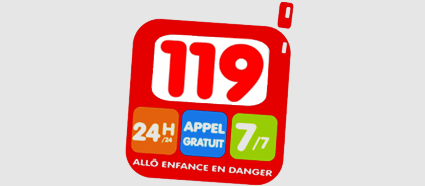
\includegraphics[width=\linewidth]{./Visuais/Ouvidorias/119-Franca.png}}\vspace{1pt}
  \\
  %\subfloat[Aruba\label{fig:Aruba}\vspace{-3pt}]{
\includegraphics[width=\linewidth]{./Visuais/Ouvidorias/131-Aruba.png}}\vspace{1pt}
  \\
  \subfloat[Japão\label{fig:Japao}\vspace{-3pt}]{
\includegraphics[width=\linewidth]{./Visuais/Ouvidorias/189-Japao.png}}\vspace{1pt}
  \\
  \subfloat[Índia\label{fig:India}\vspace{-3pt}]{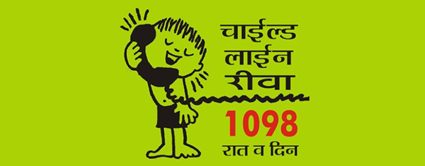
\includegraphics[width=\linewidth]{./Visuais/Ouvidorias/1098-India.png}}\vspace{1pt}
  \\
  \subfloat[Tailândia\label{fig:Tailandia}\vspace{-3pt}]{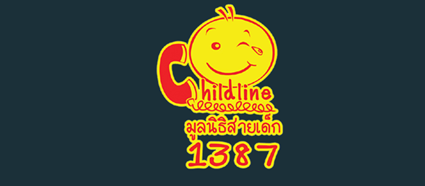
\includegraphics[width=\linewidth]{./Visuais/Ouvidorias/1387-Thailandia.png}}\vspace{1pt}
  %\begin{center}
  %  
\includegraphics[width=\linewidth]{./Visuais/Ouvidorias/100-Brasil.png}
  %\end{center}
  %\begin{center}
  %  
\includegraphics[width=\linewidth]{./Visuais/Ouvidorias/102-Argentina.png}
  %\end{center}
  %\begin{center}
  %  
\includegraphics[width=\linewidth]{./Visuais/Ouvidorias/131-Aruba.png}
  %\end{center}
  %\begin{center}
  %  
\includegraphics[width=\linewidth]{./Visuais/Ouvidorias/111-Vietna.png}
  %\end{center}
  %\begin{center}
  %  
\includegraphics[width=\linewidth]{./Visuais/Ouvidorias/189-Japao.png}
  %\end{center}
  %\begin{center}
  %  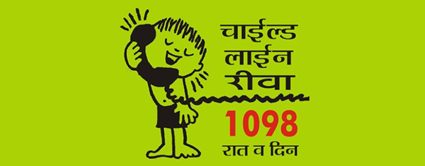
\includegraphics[width=\linewidth]{./Visuais/Ouvidorias/1098-India.png}
  %\end{center}
  %\begin{center}
  %  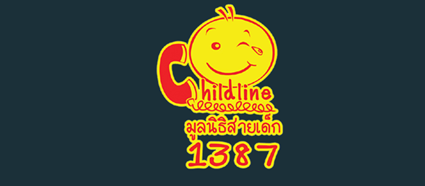
\includegraphics[width=\linewidth]{./Visuais/Ouvidorias/1387-Thailandia.png}
  %\end{center}
  %\begin{center}
  %  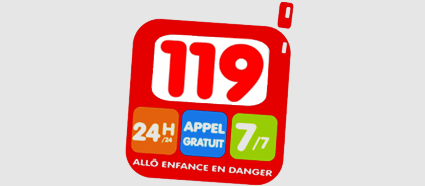
\includegraphics[width=\linewidth]{./Visuais/Ouvidorias/119-Franca.png}
  %\end{center}
  \legend{Fonte: \citeonline{UNICEF2017new}.}%eu paguei outros nao citados aqui, como fazer a referencia?
  %india (mas não governamental)
\end{wrapfigure}

Os canais de denúncia são uma estratégia relevante no combate a violência sexual infantil. Os meios de comunicação para delação servem de alicerce para garantir os direitos legalmente estabelecidos das crianças e dos adolescentes. Entre os meios de denúncia mais amplamente presentes pelo mundo estão as linhas telefônicas. A \autoref{fig:Canais} elenca as principais ouvidorias telefônicas de alguns países.

Os números telefônicos da \autoref{fig:Canais} demonstram a preocupação dos países em garantir um canal seguro de comunicação para crianças em situação de risco. A depender do país, cada canal de comunicação pode aceitar outras formas de denúncia, além da violência infantil. No caso do Brasil, o Disque 100 (\autoref{fig:Brasil}), além de receber denúncias contra crianças, também recebe denúncias de outros grupos vulneráveis como idosos e deficientes. Os meios de denúncia veem no intuito de mitigar as lacunas deixadas pelas políticas públicas no que diz respeito a fiscalização.

Os canais telefônicos são instrumentos de denúncia a distância confiáveis e acessíveis \cite{UNICEF2017new}. A penetrância dos dispositivos móveis no Brasil, torna este instrumento ainda mais poderoso no combate a violência infantil, uma vez que a quantidade de dispositivos móveis operantes no país ultrapassa a própria população brasileira. Além das denúncias por ouvidorias telefônicas, as denúncias podem ser realizadas por correio eletrônico, aplicativos e portais governamentais. As denúncias no Brasil podem ser realizadas de forma totalmente gratuita durante toda a semana 24 (vinte e quatro) horas por dia (incluindo sábados, domingos e feriados).

Os canais de denúncia fortalecem as política públicas de enfrentamento e combate a violência sexual infantil. As linhas de atendimento infantil permitem que crianças e jovens encontrem um caminho para sua segurança e bem-estar. Os canais de denúncia são fontes confiáveis e acessíveis para ajudar e apoiar crianças e jovens em situação de risco, além de encaminhá-los para os devidos sistemas nacionais de proteção a infância e a adolescência \cite{UNICEF2017new}.

%-------------------------------------------------------------------------------------------------------------------

\section{Canais de Divulgação}\label{sec:propagandas}

Os canais de divulgação são indispensáveis para a disseminação de informações substânciais para se combater a violência sexual infantil. Os meios de divulgação ajudam na dispersão do conhecimento e na conscientização da população. Os programas de conscientização da população são largamente conhecidos por auxiliarem suas respectivas lutas. %seja em capampanhas de vacinação ou em campanhas de combate a mosquitos transmissores de doenças. 
No caso da violência sexual infantil, ações publicitárias auxiliam as crianças sobre seus direitos ensinando-as e encorajando-as a realizarem denúncias. Um exemplo de ação publicitária neste estilo é apresentado na \autoref{fig:ad}.

\begin{figure}[htb]%
  \centering
  \caption{\label{fig:ad}Propaganda de consientização contra a violência sexual infantil.}%
  \subfloat[\centering \label{fig:adulto}Propaganda na visão do Adulto.]{{\frame{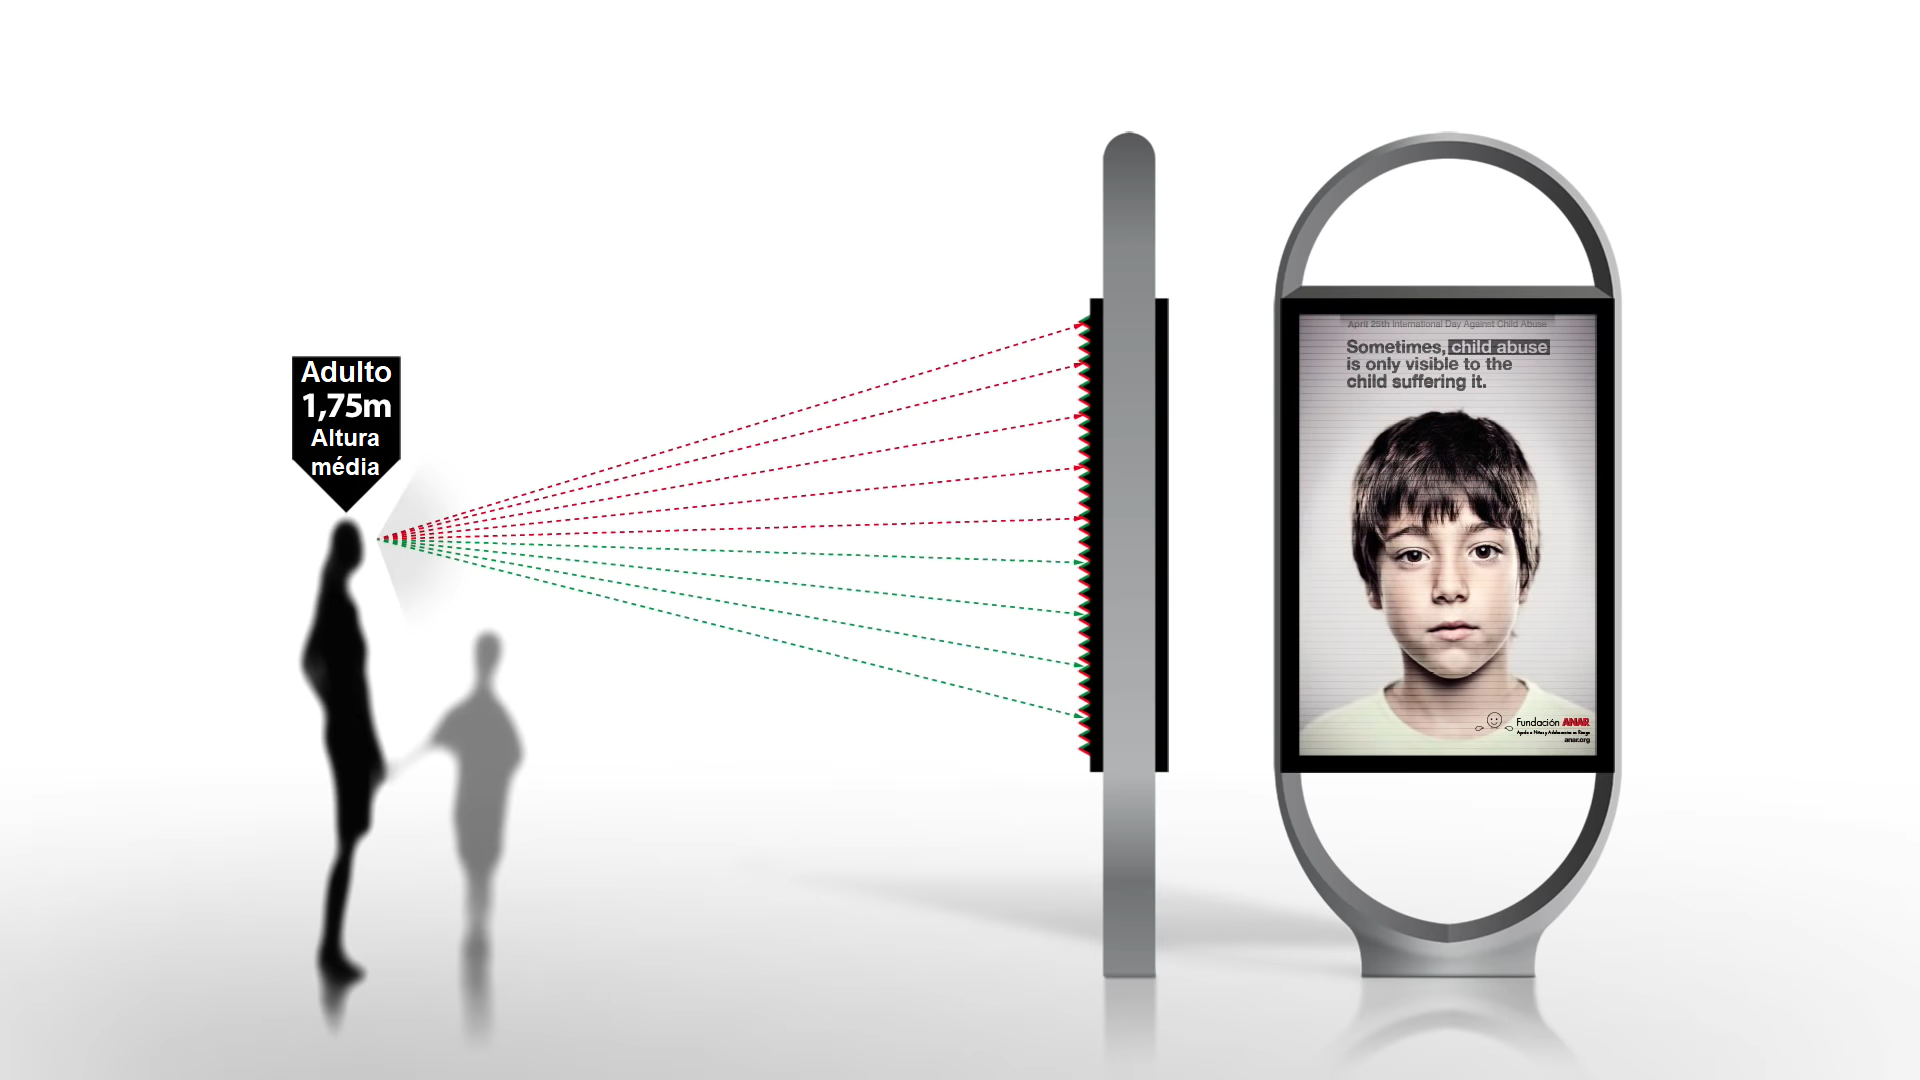
\includegraphics[width=0.48\linewidth]{./Visuais/Propagandas/Propaganda-Adulto.png}}}}%
  \hspace{0.01cm}
  \subfloat[\centering \label{fig:crianca}Propaganda na visão da Criança.]{{\frame{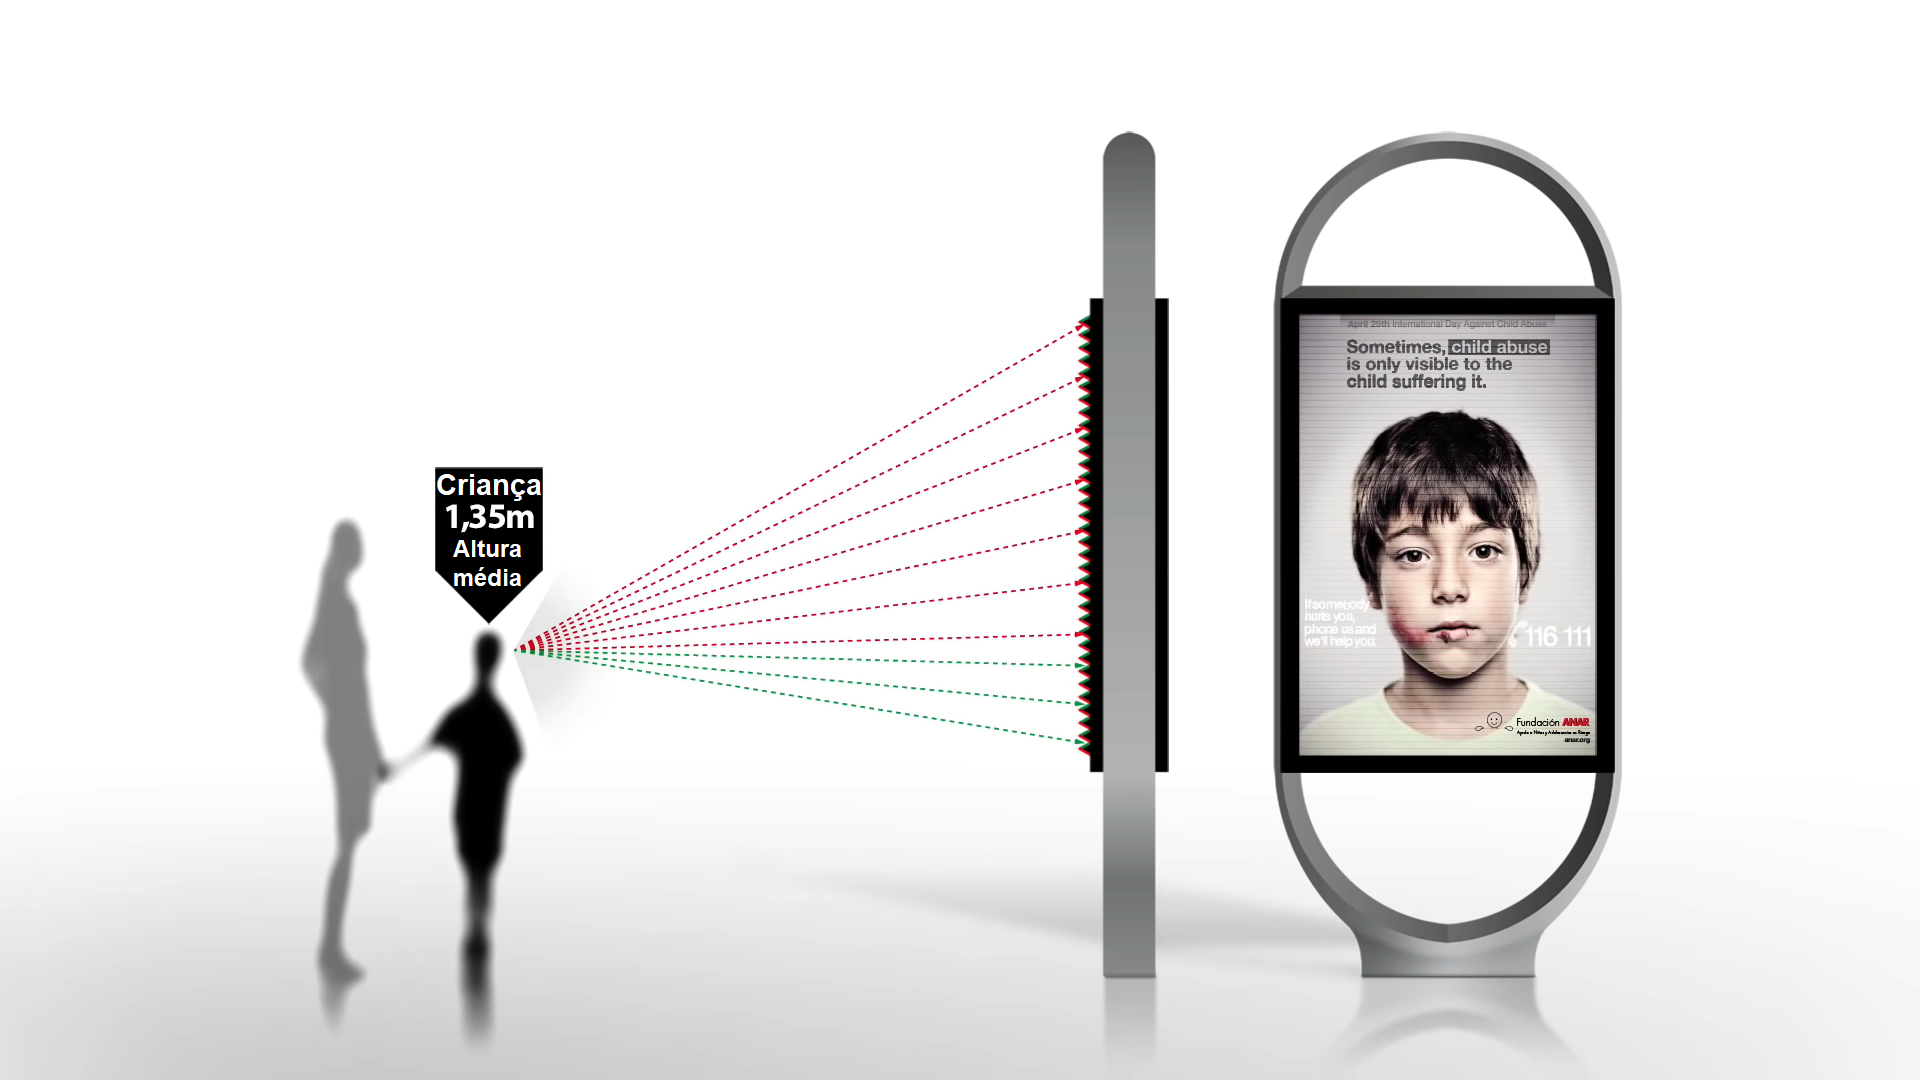
\includegraphics[width=0.48\linewidth]{./Visuais/Propagandas/Propaganda-Crianca.png}}}}%
  \vspace{10pt}
  \legend{Fonte: adaptado de \citeonline{anar2013campana}.}
  \label{fig:example}%
\end{figure}

A \autoref{fig:adulto} e a \autoref{fig:crianca} apresentam a mesma propaganda, porém vista de ângulos diferentes. A propaganda parte da concepção de que muitas crianças violentadas transitam pelas ruas com seus próprios agressores. Agressores estes, que para não serem encarcerados garantem o desconhecimento da criança sobre os meios de denúncia relativos ao crime cometido. A propaganda então, baseada sob estes princípios, apresenta uma mensagem visível apenas a partir do ângulo de visão da altura média de uma criança (1,35 metros). A mensagem, dentre outras informações, apresenta aos menores um número telefônico, o qual permite um canal de ajuda e socorro as crianças vítimas de violência. 

As ações publicitárias auxiliam na divulgação de informações, as quais capacitam as pessoas a reconhecerem o problema e a reagirem adequadamente ao problema. Os meios de divulgação são os mais variados, podendo ir desde comerciais no rádio, na televisão ou na \textit{internet} \cite{martinez2000prevencion}. Além disso, excelentes meios de divulgação são cartazes, panfletos, cartilhas e campanhas governamentais \cite{mendelson2015parent}. A extensão dos meios de divulgação possibilita que indivíduos em situação de risco possam vir a conhecer melhor sobre seus direitos. Desta forma, os meios de comunicação se assentam como uma peça chave na luta contra os maus-tratos infantis. 

%-------------------------------------------------------------------------------------------------------------------

\section{Atendimento Hospitalar}\label{sec:hospital}

Os atendimentos hospitalares são procedimentos poderosos no combate aos maus-tratos contra as crianças. O profissional de saúde surge como um sujeito ativo, no sentido de identificar abusos e denunciá-los, conforme ordena a legislação brasileira \cite{Lei:8069:1990, almeida2012responsabilidade, costa2019maus}. Inúmeros jornais e portais de notícias já relataram inclusive o diagnóstico de violência sexual infantil em laudos médicos\footnote{Portal de Notícias G1 (08/08/2019): \url{https://g1.globo.com/sp/sao-jose-do-rio-preto-aracatuba/noticia/2019/08/08/pais-tiram-crianca-de-hospital-antes-de-alta-apos-medico-suspeitar-de-sinais-de-abuso-sexual.ghtml}.}\footnote{Redação de Notícias Catve.com (28/12/2018): \url{https://catve.com/noticia/9/238135/menina-de-11-anos-e-internada-com-dores-abdominais-e-medico-descobre-gravidez}.}\footnote{Portal de Notícias G1 (08/08/2018): \url{https://g1.globo.com/ro/ji-parana-regiao-central/noticia/2018/08/08/mae-leva-filha-de-5-anos-ao-pediatra-e-descobre-que-menina-foi-estuprada-em-ro.ghtml}.}\footnote{Rede Jornalística A Gazeta (03/11/2017): \url{https://www.gazetaonline.com.br/noticias/policia/2017/11/menino-contrai-sifilis-e-familia-descobre-abuso-sexual-1014106068.html}.}\footnote{Portal de Notícias G1 (12/09/2016): \url{http://g1.globo.com/mato-grosso/noticia/2016/09/crianca-de-1-ano-morre-em-hospital-e-medicos-denunciam-suposto-abuso.html}.}\footnote{Jornal Metropóles (07/06/2016): \url{https://www.metropoles.com/distrito-federal/seguranca-df/medico-denuncia-estupro-de-menina-de-11-anos-em-festa-de-escola-no-df}.}\footnote{Portal de Notícias G1 (26/08/2015): \url{http://g1.globo.com/sao-paulo/itapetininga-regiao/noticia/2015/08/mae-descobre-que-filho-foi-estuprado-apos-dentista-achar-doenca-na-boca.html}.}\footnote{Portal de Notícias G1 (23/04/2013): \url{http://g1.globo.com/sp/bauru-marilia/noticia/2013/04/exame-aponta-que-menina-de-3-anos-sofreu-abuso-sexual-em-bauru-sp.html}.}.

A literatura médica comenta sobre a dificuldade em constatar sinais de violência infantil em alguns casos. Em certas circunstâncias se exige do médico muito mais perspicácia e experiência profissional \cite{paiva2012violencia}. Devido a complexidade no diagnóstico de alguns episódios de abuso, guias clínicos foram desenvolvidos como o Guia Clínico da \aclu{OMS} \cite{OMS2017responding}. Os relatórios e guias médicos são capazes de ajudar os profissionais de saúde a identificar mais facilmente sinais de abuso acometidos contra a criança e contra o adolescente \cite{christian2015aap}.

Os guias e relatórios médicos ajudam tanto no diagnóstico, quanto na procedência dos tramites legais. Nos casos agudos e recentes de violência sexual, as medidas legais já devem acompanhar toda a assistência inicial de diagnóstico e tratamento. Nos casos crônicos e repetitivos, sem grandes lesões visíveis, devesse realizar o registro de anamnese, histórico familiar e dados de exame físico. Além disso, é fundamental a realização de um \ac{B.O.} em uma delegacia de polícia, para fins de processo judicial e para a comprovação da agressão, bem como para confecção de exames e investigações que levem à identificação devida do agressor \cite{paiva2012violencia}. 

O atendimento hospitalar adiciona mais uma camada de defesa no enfretamento a violência sexual infantil. Embora os abusos só possam ser diagnosticados após sua ocorrência, a defesa médica ainda se faz válida para diminuir a reincidência dos eventos abusivos, seja em um exame de rotina ou qualquer outra forma de atendimento \cite{costa2019maus}.

%-------------------------------------------------------------------------------------------------------------------

\section{Centros de Tratamento às Vítimas}\label{sec:centros}

Os centros de tratamento estabelecem uma poderosa estratégia de enfretamento ao maltrato infantil. No Brasil, o tratamento e recuperação da criança vítima de violência pode ser executado tanto pelo Conselho Tutelar, quanto pelo \ac{CREAS}. Os centros de tratamento surgem sob uma perspectiva de fornecer suporte e apoio necessário a indivíduos em situação de risco, tal como garantir seus direitos legalmente estabelecidos \cite{caccia2014conselheiros}.

O Conselho Tutelar é um órgão permanente e autônomo, não jurisdicional, encarregado de zelar pelo cumprimento dos direitos da criança e do adolescente \cite{brasil2002notificacao}. Já o \ac{CREAS}, é responsável pelo acolhimento e pelo atendimento a famílias e indivíduos em situação de risco pessoal e social, por violência, abuso e exploração sexual, ocorrência de abandono, maus-tratos físicos e/ou psíquicos, cumprimento de medidas socioeducativas, situação de rua e de trabalho infantil, entre outras situações de violação dos direitos.

No que tange a violência sexual infantil, os centro de tratamento operam de modo a recuperar a saúde física e mental das crianças e dos adolescente acometidos por essa forma de violência. Os menores são ouvidos e encaminhados aos seus devidos cuidados. Esse processo possibilita menores chances de revitimização desses indivíduos, diminuindo assim as taxas de violência sexual de crianças e adolescentes \cite{faraj2016atendimento}. A implementação de centros de tratamento estabelece um grande aliado na proteção dos direitos da infância e da juventude e a sua implementação no país é de extrema importância para enfrentar o problema da violência sexual contra crianças e adolescentes. 

O Conselho Tutelar não presta o atendimento direto às vítimas de violência, mas atua de forma que ele se viabilize em casos concretos de ameaça ou violação de direitos. A legislação brasileira informa inclusive que os casos de suspeita ou confirmação de maus-tratos contra criança ou adolescente devem, obrigatoriamente, ser comunicados ao Conselho Tutelar da respectiva localidade, sem prejuízo de outras providências legais. Em adendo, a lei obriga que exista pelo menos um Conselho Tutelar por município composto de pelo menos cinco membros com idoneidade moral escolhidos pela comunidade local. 

O tratamento devido, de crianças e adolescente, vítimas de violência sexual é crucial para mitigar os males causados por essa forma de violência. Ou seja, os centros de tratamento às vítimas não almejam enfrentar diretamente a questão dos maus-tratos de crianças e adolescentes, mas sim, os problemas gerados por esses maus-tratos, tais como: depressão, estresse pós-traumático e ideação suicida. Desta forma, os cuidados tomados com crianças e adolescentes vem de modo a ajudá-los a superar suas sequelas físicas ou psicológicas. Em adendo, essa política pública de tratamento ainda é capaz de estabelecer uma estratégia válida para diminuir a reincidência de eventos abusivos \cite{costa2019maus}.

%-------------------------------------------------------------------------------------------------------------------

\section{Departamentos Policiais}\label{sec:dp}

As delegacias especializadas são um bom artifício de confronto a violência sexual infantil. No Brasil, a competência para fiscalizar, investigar e instaurar inquérito e procedimentos policiais nos casos de infração penal praticada contra crianças e adolescentes é realizada pelas polícias civis. As polícias civis são de responsabilidade dos estados, sendo assim, sua estrutura organizacional e processual varia a depender da região do país \cite{rodrigues2014violencia}. Não há uma diretriz operacional única entre as delegacias especializadas a nível nacional. Algumas delegacias ficam abertas 24 (vinte e quatro) horas por dia, todos os dias da semana, enquanto outras operam apenas nos dias úteis e em horário comercial. E mesmo as abertas 24 (vinte e quatro) horas não possuem uma equipe multidisciplinar de plantão, contando com apenas os funcionários essenciais para o registro da ocorrência como agentes, escrivães e delegado \cite{brasil2016estudo}.

As delegacias especializadas no atendimento de crianças e adolescentes se dividem em duas categorias. As voltadas para o atendimento aos menores vítimas de violência e as voltadas para lidar com os menores infratores. Salienta-se que existem delegacias que conjugam essas duas funções em um mesmo órgão. Além dessa diferença legal, as delegacias podem divergir em sua estrutura no que diz respeito a presença ou não de carceragem, brinquedoteca e salas de atendimento psicológico \cite{brasil2016estudo}. Em adendo, algumas delegacias relataram inclusive convênios com hospitais, universidades e \acfp{ONG}. No entanto, independente da delegacia, todas integram o \ac{SGDCA}.

O \ac{SGDCA} compreende principalmente: os centros de defesas, as delegacias especializadas, as varas da infância e juventude, as promotorias da infância e juventude e os Conselhos Tutelares \cite{rodrigues2014violencia}. Fazer parte do \ac{SGDCA}, implica que os órgãos associados devem conferir máxima prioridade ao atendimento das crianças na faixa etária da primeira infância com suspeita ou confirmação de violência de qualquer natureza, formulando projeto terapêutico singular que inclua intervenção em rede e, se necessário, acompanhamento domiciliar. Isso faz com que todas as delegacias especializadas tenham uma estrutura em comum que atenda devidamente a esses requisitos. 

As delegacias especializadas assentam uma excelente estratégia de socorro policial aos menores sexualmente violentados. O atendimento policial ao menor vítima de violência produz uma resposta ao problema semelhante as respostas dos centros de tratamento. Contudo, as delegacias especializadas estabelecem um combate mais direto ao problema ao conduzir um processo legal para a devida identificação e apreensão do agressor. Tal ação é capaz de reduzir a quantidade de indivíduos potencialmente perigosos em circulação na sociedade, garantido assim a diminuição na incidência de eventos envolvendo a violência sexual de crianças e adolescentes. 

%-------------------------------------------------------------------------------------------------------------------

\section{Operações Policiais}\label{sec:op}

As operações policiais são excelentes alternativas na luta contra o abuso, o tráfico e a exploração sexual infantil. No Brasil e no mundo as operações são responsáveis pela busca e apreensão de inúmeros criminosos sexuais, o que acaba por mitigar a reincidência do crime por parte destes agressores.

A literatura relata a Operação Carrossel (2007) como o primeiro esforço policial internacional a combater a pornografia infantil na \textit{internet} \cite{lowenkron2014all}. Todavia, há registros anteriores que relatam a mesma abrangência policial internacional, como a Operação Catedral (1998) objetivada também no combate a pornografia infantil na \textit{internet} \cite{barrot2008brochuras, jesus2006anti}. É importante destacar que isto não se trata necessariamente de uma contradição literária, a Operação \textit{Darknet} (2014) também é descrita como pioneira no combate a distribuição de material pornográfico infanto-juvenil na \textit{internet}, contudo o pioneirismo desta, configura-se pela metodologia de investigação e pelas ferramentas para identificar usuários criminosos na \textit{Deep Web} \cite{tonello2018pedofilia}. Ou seja, cada operação pode ser classificada como pioneira com base em seus contextos específicos. 

No Brasil, o \ac{MJ} considera a Operação Luz na Infância (2017) como a maior operação de enfretamento a pornografia infantil no Brasil e na América Latina. Isto, pois a operação é um conglomerado de vários países e instituições \cite{souza2018sabemos}. Entre os países estão: Brasil, Chile, El Salvador, Equador, Estados Unidos da América, Panamá e Paraguai. A Operação Luz na Infância já teve mais de seis fases, as quais já apreenderam um volume total de dados que ultrapassa os 3 (três) \aclu{TB}, além da prisão de mais de 500 (quinhentos) indivíduos. 

As operações policiais são políticas públicas de segurança que estão fundamentadas e baseadas nos limites da legislação e da jurisdição de suas nações, resguardados os acordos internacionais. Dito isso, é notória a dependência que as operações policiais possuem com o âmbito jurídico. Se não há tipificação legal do crime, então não a crime a ser reprimido. Por tal razão que a sansão de decretos e a criação de leis neste contexto se fazem fundamentais para o fortalecimento das operações policiais. 

A dependência jurídica das operações policiais pode ser uma barreira a ser enfrentada no combate a violência sexual infantil. De nada adianta uma operação contra o abuso de crianças em um país que permite legalmente o casamento infantil. Além da barreira jurídica, as estratégias policiais sofrem do mesmo mal dos atendimentos hospitalares, uma vez que a apreensão do criminoso só pode ocorrer após a ocorrência do crime ou a tentativa dê, todavia a defesa policial ainda se faz válida para diminuir a reincidência dos eventos abusivos uma vez que os criminosos tenham sido encarcerados ou levados a tratamento. 

%-------------------------------------------------------------------------------------------------------------------

\section{Gestão de Infratores}\label{sec:infratores}

O encarceramento de criminosos sexuais é uma boa alternativa de combate ao problema da violência sexual infantil, no curto prazo. O encarceramento de agressores sexuais remove indivíduos perigosos do convívio social, além de trazer conforto e tranquilidade às suas vítimas. No entanto, o encarceramento não resolve a questão da violência sexual de crianças e adolescentes, no longo prazo.  

Há longo prazo, os agressores sexuais apresentam taxas de reincidência elevadas após sua soltura. A explicação, vem da ausência de intervenções dirigidas à problemática, durante o cumprimento da pena de prisão \cite{ribeiro2018programas, finkelhor2009prevention, maia2014castraccao}. A atitude unicamente punitiva de sistemas jurídicos, acaba por não tratar devidamente o problema do abuso sexual \cite{camila2019violencia}. Embora a atração sexual por crianças e adolescentes seja considerada uma patologia, o agressor sexual não é considerado inimputável perante a justiça, caso o delito tipificado em lei seja cometido \cite{ribeiro2018programas}. Contudo, um tratamento adequado ao agressor se faz necessário para diminuir a probabilidade da reincidência do crime. Os programas de tratamento apresentam uma taxa de sucesso alta, implicando assim em uma baixa reincidência dos crimes sexuais \cite{ribeiro2018programas}. Meta-análises apoiam inclusive os efeitos significativos de tratamentos baseados em princípios cognitivo-comportamentais \cite{mendelson2015parent}.

As terapias e os tratamentos aos agressores sexuais precisam ser realizados com muita cautela. Por mais que os delitos cometidos pelos agressores sexuais sejam desumanos e atentem contra o livre direito de suas vítimas; por questões éticas ainda se faz necessário garantir que os tratamentos e que as terapias não violem os direitos dos agressores sexuais \cite{finkelhor2009prevention}. Por tal razão terapias de aversão, choque ou tratamentos de castração química não são recomendadas por algumas instituições de saúde \cite{maia2014castraccao}. Expressar empatia e compreensão com as pessoas que cometeram violência sexual frequentemente é visto como se a atitude do abusador fosse defendida (o que é errôneo). Especialistas defendem que a humanização do agressor seja feita para a condução de um tratamento mais adequado.

A literatura relata tanto tratamentos voltados aos já infratores, quanto tratamentos voltados aos indivíduos não incidentes que são sexualmente atraídos por crianças, e que buscam ajuda para lidar melhor com sua patologia sexual \cite{finkelhor2009prevention}. Esforços de ambos os gêneros produzem efeitos promissores relatados por alguns estudos na área \cite{mendelson2015parent}.

O tratamento de indivíduos sexualmente atraídos por crianças pode ajudar que não haja novas vítimas e para que aqueles que já cometeram algum crime, não voltem a fazê-lo. Demonstram-se como um excelente meio de resolução do problema, pois o problema não é resolvido pura e simplesmente com a punição do agressor, mais sim, com o seu tratamento. 

%-------------------------------------------------------------------------------------------------------------------

\section{Programas de Capacitação}\label{sec:programas}

Os programas de capacitação demonstram-se como uma excelente alternativa para o enfrentamento aos maus tratos contra os menores. O processo de capacitação busca instruir determinados indivíduos sobre um certo âmbito. No caso da violência infantil, de modo geral os programas buscam ensinar um conjunto de indivíduos a identificar e reagir adequadamente ao problema. 

Os processos de capacitação podem envolver desde uma grande comunidade até grupos específicos de indivíduos. Neste sentido, a atual seção apresenta os três grupos mais corriqueiramente relatados pela literatura na área: os pais/responsáveis das crianças (\autoref{ssec:pais}), os profissionais que trabalham com crianças (\autoref{ssec:professores}) e as próprias crianças (\autoref{ssec:alunos}).

\vspace{1.0 cm}
\subsection{Pais/Responsáveis}\label{ssec:pais}

Os programas sobre sexualidade para pais/responsáveis buscam, no geral, conscientizá-los sobre os cuidados necessários para que suas crianças tenham um risco menor de sofrer qualquer tipo de violência sexual \cite{pelisoli2010prevenccao}. Essa conscientização pode vir por meio de programas voltados para a instrução de pais/responsáveis, ou de projetos voltados para a conscientização de pais/responsáveis a respeito dos programas infantis. 

Os programas voltados a instrução de pais/responsáveis se baseiam em preencher algumas lacunas de conhecimento, trazendo assim, mais informações no âmbito da violência infantil para pais ou responsáveis \cite{maria2010papel}. A ideia de tais programas é desmistificar alguns mitos relacionados a temática da violência sexual infantil, assim como fornecer informação adequada, recursos práticos e dar apoio.

Os projetos voltados para a conscientização de pais/responsáveis a respeito dos programas infantis estão normalmente associados a programas de educação em sexualidade para crianças. Muitos guardiões legais se preocupam com os programas preventivos de cunho sexual ministrados as suas crianças, pois temem que estes programas possam levar as crianças a saberem muito sobre sexo, depravando-as de alguma forma \cite{chen2007prevention}. Sendo assim, os projetos de conscientização para pais/responsáveis vêm no intuito de prestar esclarecimento de modo a tornar os programas de educação sexual para crianças menos restritivos. 

Programas parentais sobre sexualidade demonstram resultados promissores na redução dos maus-tratos infantis \cite{silverman2008evidence}. Embora os dados indiquem que a maior parte dos maus-tratos de crianças e adolescentes advém dos próprios responsáveis legais da criança, os programas ainda se fazem válidos para aqueles que buscam trazer maior segurança e proteção para suas crianças \cite{pelisoli2010prevenccao}.

\subsection{Profissionais}\label{ssec:professores}

Treinar profissionais que trabalham com crianças para o reconhecimento e enfretamento do \ac{ASI} é uma boa estratégia para se combater a violência contra as crianças. Entre os profissionais a serem treinados estão principalmente os: médicos, professores e policiais. Os médicos são treinados a diagnosticarem de forma mais rápida e adequada os casos de violência infantil \cite{paiva2012violencia}. Os professores são ensinados de modo a torná-los mais comprometidos com os programas de educação sexual para crianças \cite{colleen2016advancing}. Já os policiais são instruídos a agir de maneira efetiva as denúncias realizadas \cite{pelisoli2010prevenccao}. 
%os próprios gestores reconhecem o despreparo dos profissionais, a precariedade de recursos, a ineficiência dos encaminhamentos e a falta de articulação entre diferentes setores que atuam nessa área. \cite{pelisoli2010prevenccao}
Um programa que abrange esses três tipos de profissionais é o Programa Criança Protegida. 

O Programa Criança Protegida tem o objetivo de capacitar conselheiros tutelares, agentes de saúde, policiais, guardas municipais, professores e outros profissionais ligados à garantia dos direitos da criança e do adolescente no enfrentamento de violações, principalmente os crimes de abuso sexual contra vulneráveis \cite{oei2020tomada}. Infelizmente, o alcance bibliográfico da atual pesquisa não foi capaz de encontrar estudos conclusivos que atestassem a eficácia do treinamento de todos estes profissionais no combate ao abuso infantil. Todavia, falando especificamente dos profissionais ligados a educação, pesquisas já confirmam a eficácia no treinamento de professores ligados a programas de educação sexual infantil \cite{colleen2016advancing}. 

\subsection{Alunos}\label{ssec:alunos}

A educação sexual infantil é uma boa forma de prevenir a violência sexual de crianças e adolescentes \cite{finkelhor2009prevention}. Os programas preventivos para crianças buscam educar os menores a reconhecerem e a responderem adequadamente a episódios abusivos, evitando assim, que a violência aconteça. Os programas educacionais para a prevenção da violência sexual infantil podem abranger desde as crianças da mais tênue idade até adolescentes quase entrando em sua vida adulta. Os programas voltados a educar as menores faixas etárias são os mais criticados, por responsabilizarem demasiadamente a criança \cite{colleen2016advancing}. Nesses programas, existe a preocupação da criança culpar a si mesma após um episódio de violência, por não ter evitado o abuso, possivelmente agravando ainda mais os traumas deixados no menor. Existem outras críticas feitas a tais programas, devido a sua temática sensível e delicada \cite{scholes2014serious}. Todavia os programas educacionais para crianças estão entre as melhores iniciativas de combate à violência infantil \cite{barron2008school, finkelhor2009prevention}.

A eficiência dos programas infantis na prevenção da violência sexual, advém de um fato conhecido na história da área. Historicamente, sabe-se que os agressores sexuais preferem atuar sobre crianças com menores chances de manifestarem resistência aos seus abusos, tais crianças são classificadas pelos agressores sexuais como sendo a \textit{vítima ideal} \cite{budin1989sex}. Portanto, a instrução e capacitação de crianças nessa temática diminui a quantidade de \textit{vítimas ideais} presentes na sociedade, coibindo assim, os predadores sexuais de praticarem seus delitos.


\section{Materiais de Ensino}\label{sec:materiais} 

Os materiais de ensino são grandes aliados do processo pedagógico. Os materiais englobam no geral, toda a classe de dispositivos e utensílios que auxiliam a obtenção de conhecimento sobre um determinado assunto. No âmbito da violência infantil, os materiais de ensino funcionam como ótimas ferramentas de reforço aos ensinos preventivos da área. A prevenção nesse sentido, pode ser atingida através do estudo individual dos materiais ou através do seu uso em programas educacionais infantis (como forma de complemento aos programas).

Os materiais didáticos vêm de modo a aprimorar o processo pedagógico. Os materiais funcionam não apenas como um instrumento facilitador do aprendizado infantil, mas também como uma ferramenta de auxílio aos professores. Entre os materiais didáticos de maior predominância ao longo da história, estão os livros.

Programas baseados em livros de educação sexual infantil, permitem a visualização mais acurada e precisa dos conceitos ensinados, na mesma medida que proporcionam listas de exercícios e atividades para o fortalecimento de tais conceitos \cite{maria2010papel}. O aprendizado pode ser complementado não apenas com livros, mas também com vídeos.

Os vídeos são ótimos materiais de ensino pois, diferentemente dos livros, proporcionam um conteúdo dinâmico com fluidez e movimentação, o que acaba por fortalecer o processo pedagógico \cite{maria2010papel}. Há ainda o fato de que os vídeos abrem um canal sonoro de comunicação, aumentando assim a retenção e a aprendizagem. No âmbito sonoro, salienta-se também a utilização de músicas no contexto da prevenção à violência sexual infantil.

Diferente dos livros e dos vídeos, as músicas são normalmente mais utilizadas em terapias para o tratamento de crianças violentadas. Terapias musicais estão relacionadas com uma autoimagem mais positiva e um melhor desenvolvimento da autoestima. O processo terapêutico com auxílio de músicas é capaz de ajudar as crianças a se sentirem melhor com elas mesmas, ajudando-as assim, em sua recuperação \cite{robarts2003healing}. Além das músicas, dos vídeos e dos livros ainda é possível citar os jogos de tabuleiro como um material de apoio a educação preventiva da violência sexual (os jogos digitais são abordados separadamente no \autoref{ssec:TR}).

Jogos de carta, tabuleiro e até mesmo atividades em papel, são utilizados como um instrumento lúdico na aprendizagem infantil. O ambiente recreativo dos jogos permite que assuntos sensíveis e delicados possam ser abordados de maneira mais divertida e natural. Devido a essas características, especialistas consideram as abordagens educativas baseadas em jogos extremamente benéficas para o ensino preventivo da violência sexual \cite{meyer2017analise}.

%Jogos de um modo geral são capazes de fortalecer o processo pedagógico. Os jogos são uma via que possibilita que assuntos difíceis, sensíveis ou embaraçosos possam ser abordados de uma forma lúdica, permitindo a diversão associada a aprendizagem \cite{stieler2016paper}. 

Os materiais de ensino se estabelecem como boas estratégias no combate a violência sexual de crianças e adolescentes. Livros, vídeos, músicas e jogos são capazes de educar crianças e jovens a se protegerem de eventuais episódios de abuso. Para os abusos já consumados, tais materiais ainda se estabelecem como fortes aliados para a realização de denúncias e para o tratamento das vítimas. 

%-------------------------------------------------------------------------------------------------------------------

\section{Considerações Finais do Capítulo}\label{sec:finais}

As estratégias elencadas por esse Capítulo são iniciativas que surgiram como resposta ao problema da violência sexual de crianças e adolescentes. Cabe destacar que todas as iniciativas aqui apresentadas advêm de inúmeras fontes literárias. Não há portanto, uma única fonte de pesquisa citada por este trabalho que agrega todas as soluções aqui apresentadas. Um compilado de todas as iniciativas apresentadas neste Capítulo é ilustrado no infográfico da \autoref{fig:Metodos}.

\vspace{0.5cm}

\begin{figure}[htb]
	\caption{\label{fig:Metodos}Principais Métodos de Combate ao Problema do Abuso Sexual Infantil.}\vspace{-0.4cm}
  \begin{adjustwidth}{-4.2cm}{-0.0cm}
    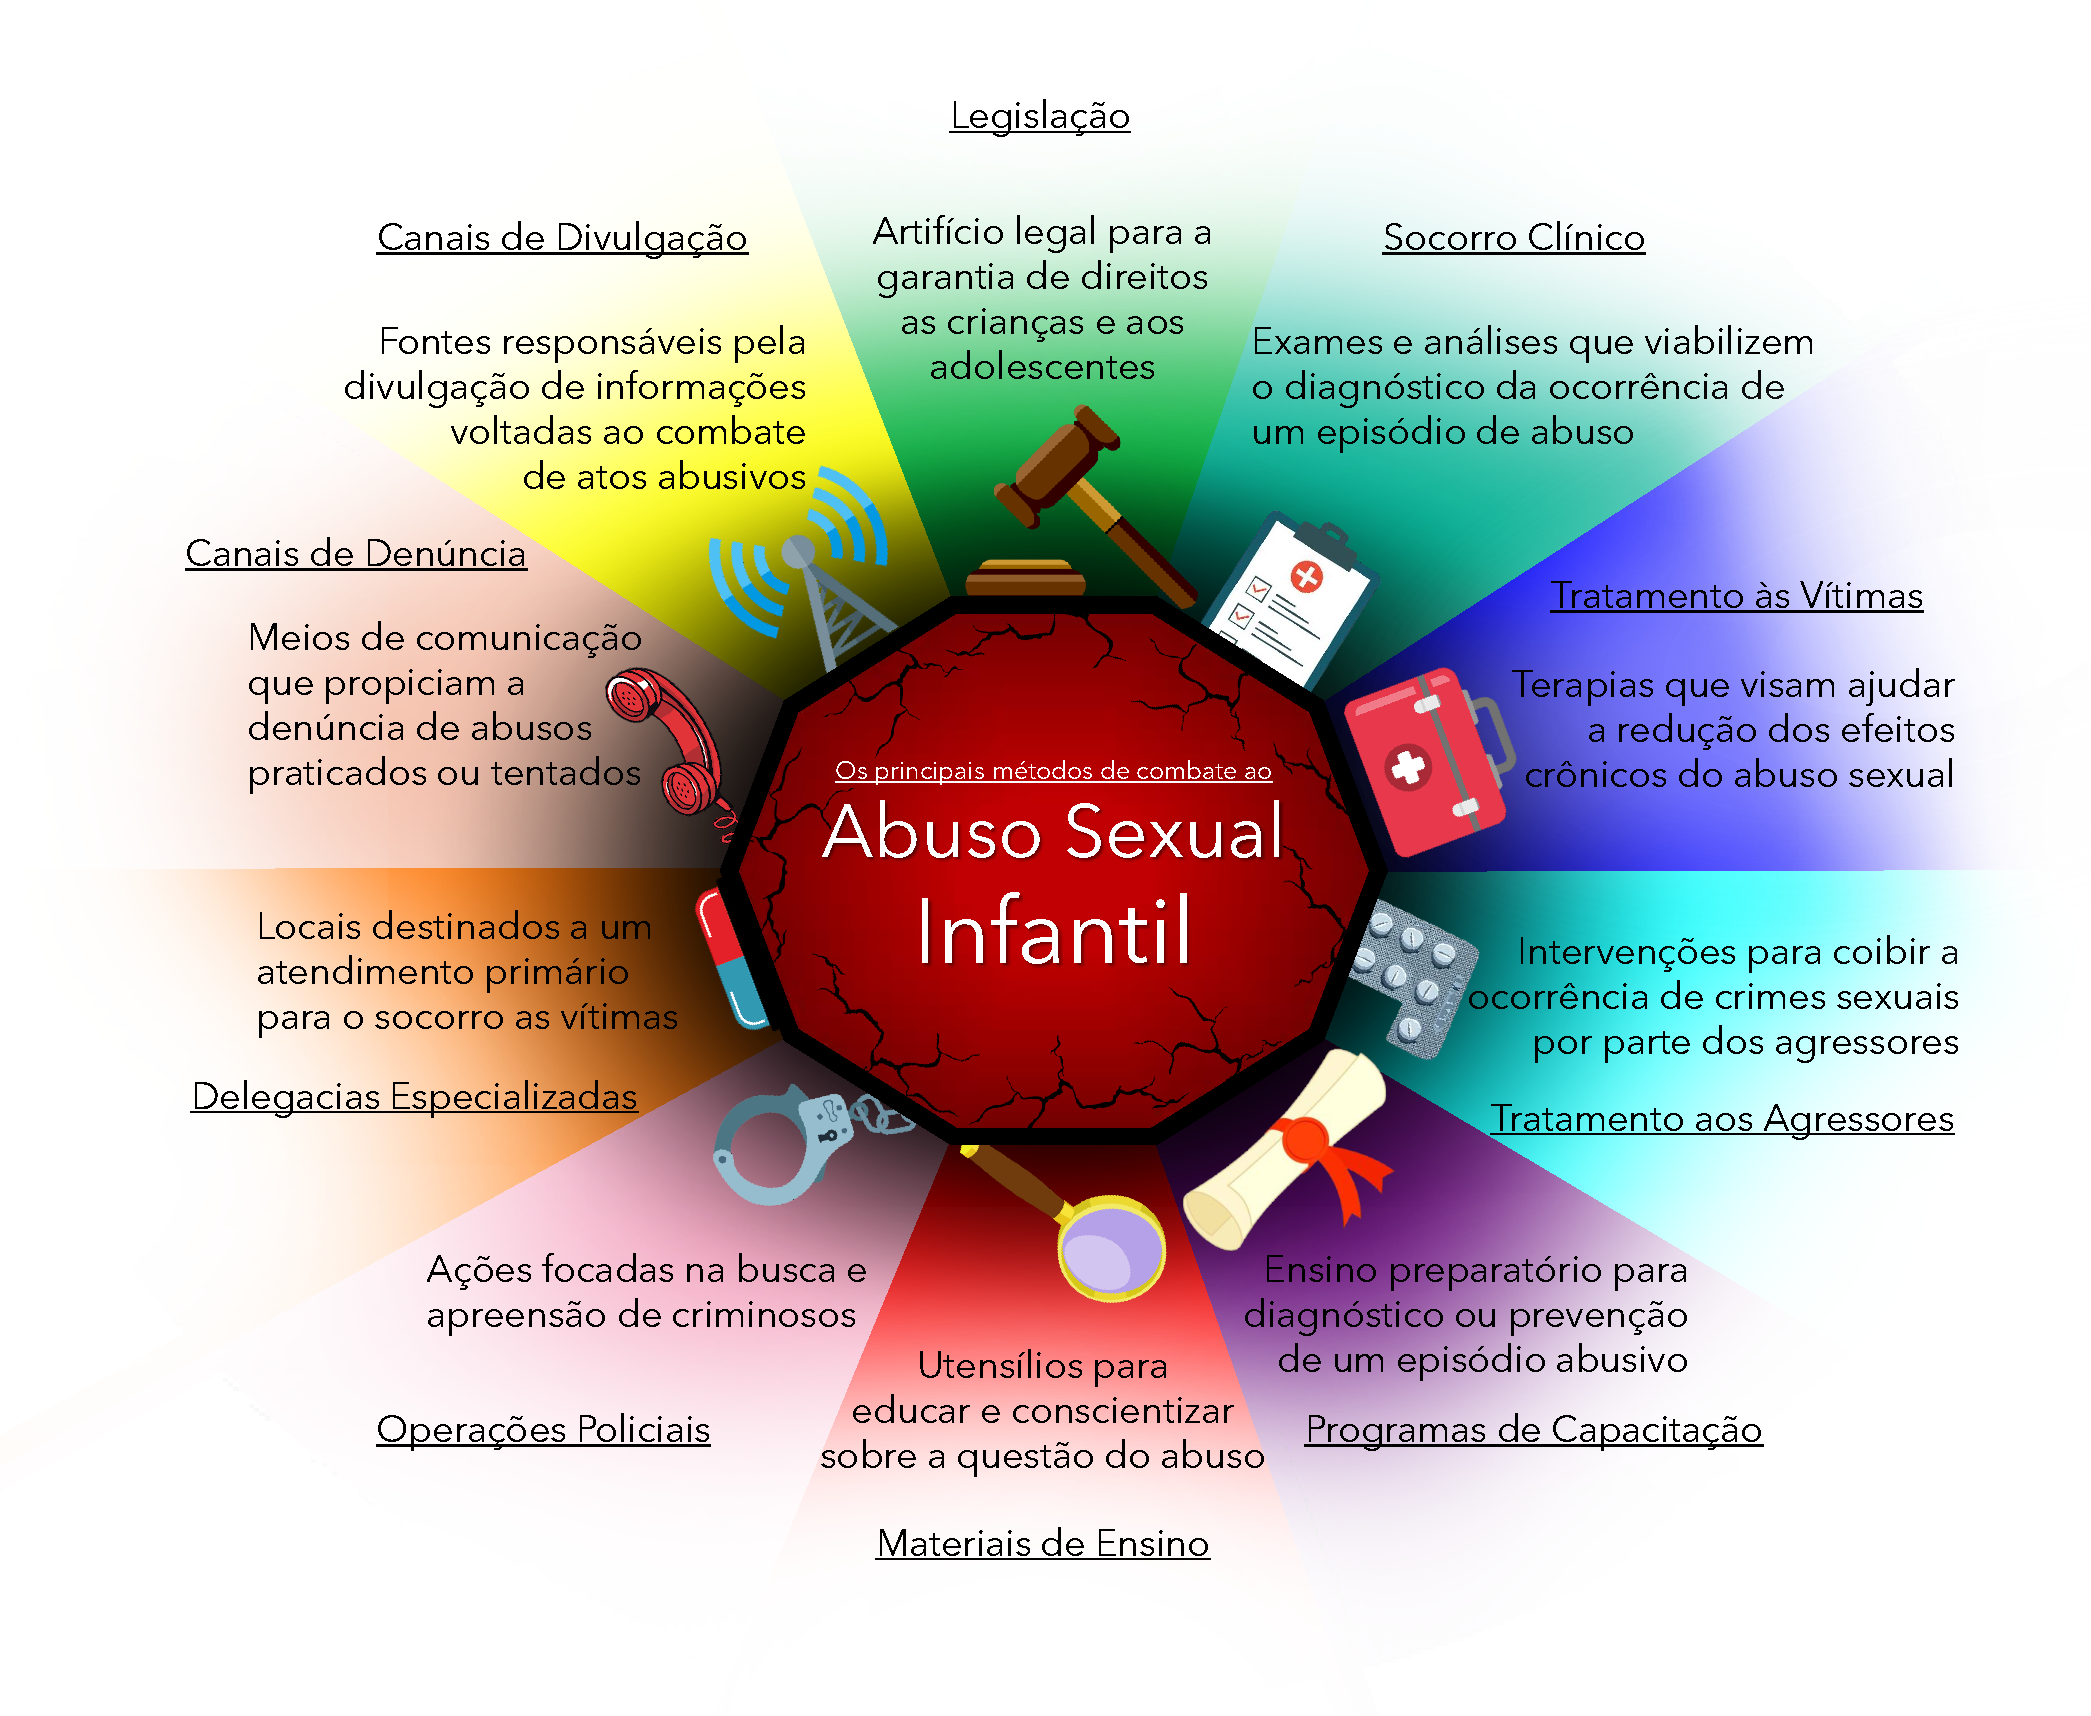
\includegraphics[scale=0.65]{./Visuais/MétodosCombate.pdf}
	\end{adjustwidth}\vspace{-1.0cm}
  \legend{Fonte: Elaborada pelo autor (2020).}
\end{figure}

A \autoref{fig:Metodos} ilustra as estratégias de combate a violência sexual infantil apresentadas neste trabalho. No âmbito jurídico foram criadas medidas legislativas (\autoref{sec:regras}), focadas no fortalecimento dos artifícios legais para o combate a violência sexual de crianças e adolescentes, dentre estes artíficíos legais cita-se a criação de inúmeros meios para a denúncia de criminosos (\autoref{sec:canais}). Para conscientizar as pessoas de seus direitos e dos meios de denúncia, surgiram os canais de divulgação (\autoref{sec:propagandas}). Aos já molestados, medidas surgiram em resposta, voltadas ou ao diagnóstico clínico (\autoref{sec:hospital}) ou ao tratamento das vítimas (\autoref{sec:centros}). Na esfera policial foram criadas as delegacias de atendimento (\autoref{sec:dp}) e as operações policiais (\autoref{sec:op}) que acabam por fornecerem uma resposta de combate direto ao problema da violência sexual infantil. Para os infratores, surgiram iniciativas voltados ao seu tratamento  (\autoref{sec:infratores}). No aspecto socioeducativo foram criados programas de capacitação (\autoref{sec:programas}), os quais podem ser complementados por materiais de ensino (\autoref{sec:materiais}), proporcionando assim, um sistema educativo capaz de conscientizar as pessoas sobre a violência sexual de crianças e adolescentes. 

A violência sexual infantil é um grave problema presente na sociedade. Em resposta a este problema sugiram inúmeras medidas nas mais diversas áreas. Por tal razão, este é o tipo de crime que não pode ser abordado numa perspectiva individual, mas sim, abordado em um contexto interdisciplinar e intersetorial \cite{maria2010papel, pinto2017avaliaccao}. É importante que as estratégias de combate a violência sexual infantil estejam em sincronia para terem seus resultados positivos maximizados. O trabalho conjunto das estratégias de combate ao abuso sexual de crianças possibilita uma tática sólida de enfrentamento ao problema, a qual é capaz de minimizar os fatores de risco para a ocorrência do problema (\autoref{fig:Riscos}), a qual é capaz de agir diretamente nos elementos de maior influência para a incidência do crime (\autoref{fig:Crime}), e a qual, é capaz de atuar em todos os instantes do crime (\autoref{fig:prevencao}).

As estratégias elencadas por esse Capítulo não representam a totalidade de estratégias existentes nesse cenário de combate a violência sexual infantil. Soluções muito abrangentes ou soluções muito vagas não foram apresentadas neste trabalho. O agrupamento de soluções, aqui apresentado, é uma visão pessoal do autor dessa dissertação e portanto, única na literatura. O agrupamento realizado dá ênfase aos critérios que nomeiam uma determina solução, elencando seus principais achados e atestando seu êxito conforme as pesquisa na área apontam.

As estratégias de combate a violência sexual infantil podem ser agrupadas de inúmeras formas. Não há registros na literatura especializada que apontem para um agrupamento único e consolidado de estratégias. Todavia, existem propostas de agrupamentos, diferentes do agrupamento apresentado neste trabalho, constituídos inclusive, por estratégias aqui não listadas. Para uma melhor compreensão da temática tratada por esta pesquisa; a leitura desses agrupamentos e compilados de estratégias é mais do que recomendada: \citeonline{australia2000preventing}, \citeonline{sanderson2004child}, \citeonline{finkelhor2009prevention} e \citeonline{inspire2016seven}.

%-------------------------------------------------------------------------------------------------------------------

\chapter{Trabalhos Relacionados}\label{ssec:TR}

\acfp{JS} são utilizados no processo ensino-pedagógico desde o início da década de \citeyear{clark1970serious}. A partir da década de \citeyear{clark1970serious}, diversos estudos foram conduzidos de modo a identificar os reais impactos que tais jogos tinham no ensino infantil e juvenil \cite{stieler2016paper}. Ao longo dos anos, cientistas e pesquisadores concluíram que a utilização de jogos em sala de aula desencadeava um aumento expressivo no desempenho escolar dos estudantes \cite{wentzel1998social}. O aumento se acentuava mais nas disciplinas relacionadas, de alguma forma, aos conteúdos ministrados pelo jogo. A utilização de jogos em sala de aula é capaz de amplificar os efeitos da aprendizagem escolar \cite{jones2020serious}. Contudo, mesmo com os jogos apresentando resultados positivos na aprendizagem infantil, \acp{JS} ainda apresentam baixas taxas de uso no ensino didático das crianças e dos adolescentes. 

A baixa adoção dos jogos no ambiente escolar pode assumir três causas. A primeira está relacionada com a inexistência de jogos apropriados a uma determinada disciplina. A segunda está ligada com a inaptidão de alguns professores em incorporar os jogos a seus planos de ensino. E a terceira está associada com a falta de equipamentos apropriados nas escolas \cite{colleen2016advancing}. Há ainda uma quarta causa impeditiva relacionada diretamente aos jogos de temática preventiva a violência sexual infantil. No caso, a temática sensível e os tabus sociais que permeiam tais jogos acabam por dificultar sua adoção em salas de aulas \cite{chen2007prevention}. Estes fatores acabam por dificultar a adoção de jogos de caráter educativo no processo de ensino, o que poderia explicar o baixo número de \acp{JS} retornados durante a execução da etapa bibliográfica deste trabalho.

Ao se tratar de jogos voltados para prevenção da violência sexual infantil, a literatura pesquisada revela uma quantidade simplória de jogos relacionados a essa temática. Desta quantidade, poucos são os jogos que foram validados por um processo rigoroso de análise e experimentos acadêmicos. Sendo assim, poucos são os jogos capazes de atestar cientificamente resultados positivos relacionando a aprendizagem e a diminuição das taxas de violência sexual de crianças \cite{jones2010being}.

O atual Capítulo dá ênfase aos três jogos de maior relevância identificados de acordo com a literatura pesquisada. Deste modo, a \autoref{sssec:Being} aborda sobre o jogo \textit{Being Safety Smart}, a \autoref{sssec:Orbit} discorre sobre o jogo \textit{Orbit Rescue} e a \autoref{sssec:CeS} discute sobre o jogo \textit{Cool and Safe}. Tais jogos se destacam também por utilizarem o questionário \ac{CKAQ} em seus experimentos, possibilitam que uma comparação mais acurada entre as pesquisas possa ser realizada. Desta forma, a \autoref{sssec:finais} realiza um breve comparativo entre tais jogos. Por fim, a \autoref{sssec:outros} lista outros jogos na mesma temática com menor rigor científico, além de dar as conclusões finais do presente Capítulo. 

%-------------------------------------------------------------------------------------------------------------------

\section{Being Safety Smart}\label{sssec:Being}

\textit{Being Safety Smart}\footnote{\textit{Being Safety Smart} é um jogo  da Universidade de Sunshine Coast lançado em fevereiro de 2009. No momento da redação deste trabalho o portal do jogo encontra-se fora do ar. No entanto a página virtual do jogo ainda pode ser acessada por meio de bibliotecas digitais voltadas a manter um acervo de páginas públicas do mundo virtual. Para ter acesso ao jogo basta recorrer a uma desta bibliotecas digitais e pesquisar pelo antigo portal do jogo: \url{http://www.beingsafetysmart.com.au}.} é um jogo digital projetado para combater o sequestro e a violência sexual de crianças. O jogo é voltado para crianças de 6 (seis) a 8 (oito) anos. O jogo almeja capacitar as crianças de modo que elas respondam adequadamente ao problema da violência sexual infantil \cite{jones2008online}. Para isso, o jogo aborda  o problema do abuso e do sequestro de crianças por meio de oito níveis distintos voltados para o fortalecimento da segurança pessoal das crianças. Os oito níveis são ministrados unicamente em língua inglesa, os quais podem ser visualizados na tela principal do jogo, ilustrada na \autoref{fig:BSS1}. 

\begin{figure}[htb]
  %\vspace{-0.5cm}
	\caption{\label{fig:BSS1}Tela Principal do jogo \textit{Being Safety Smart}.}
  \begin{center}\vspace{-0.3cm}
    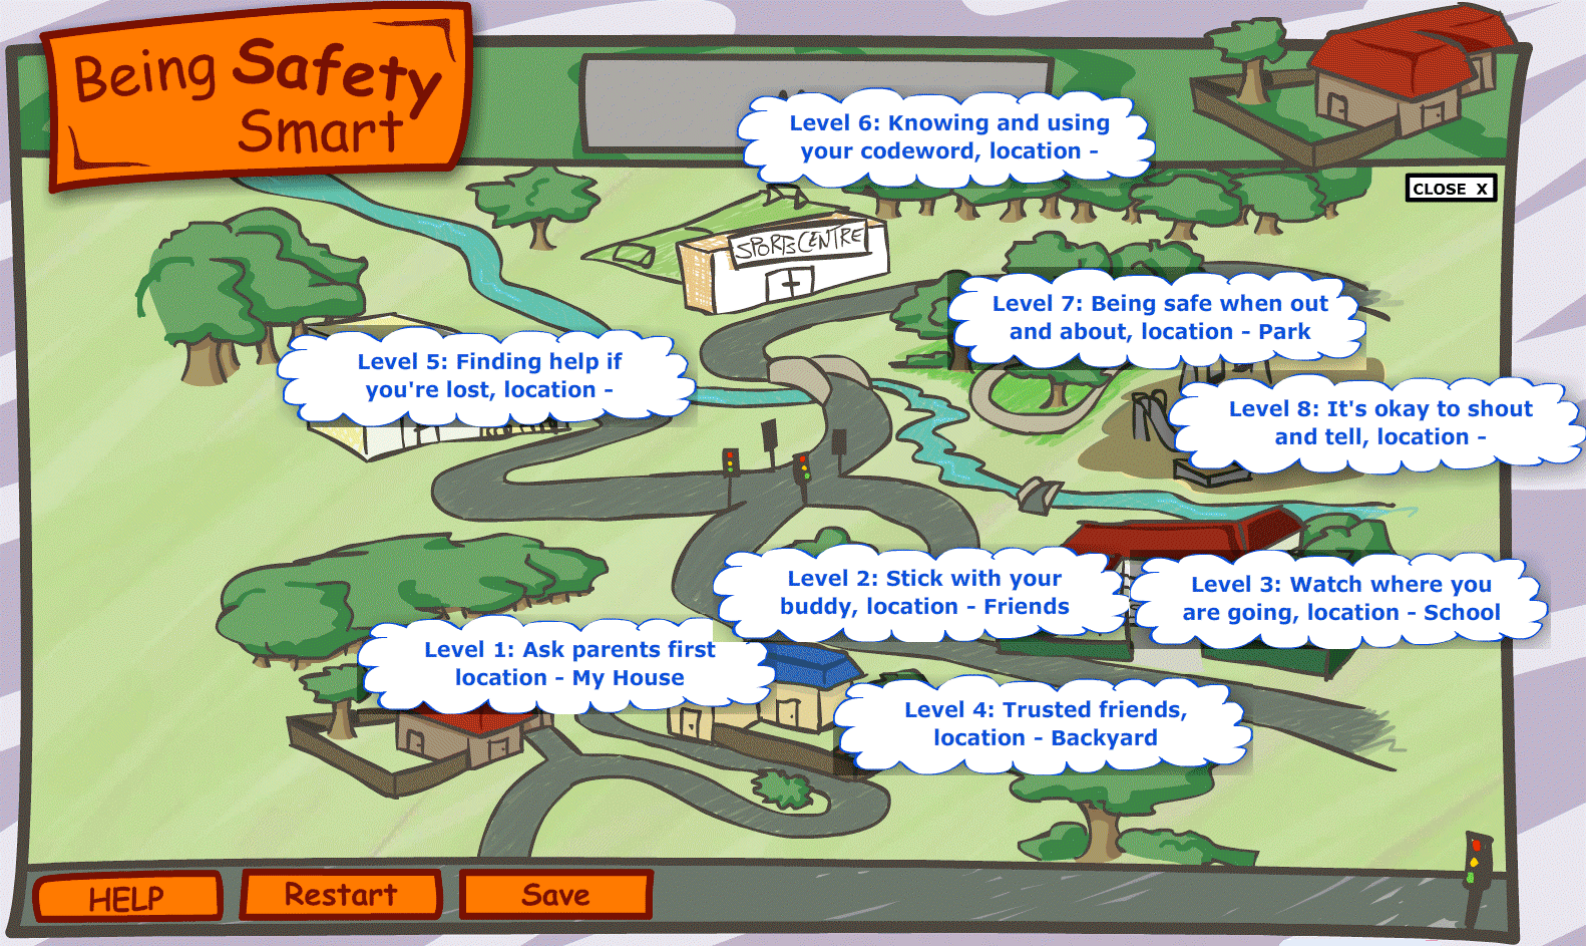
\includegraphics[width=\linewidth]{./Visuais/BSS/B1.png}
	\end{center}\vspace{-0.2cm}
  \legend{Fonte: \citeonline[p. 3]{jones2008online}}
\end{figure}

\vspace{-0.3cm}

A \autoref{fig:BSS1} apresenta a tela principal do jogo \textit{Being Safety Smart}. Oito níveis com diferentes conteúdos didáticos são mostrados nesta tela. Cada nível assume a representação de um ambiente do mundo real. O ambiente representado se relaciona de alguma forma com os assuntos a serem ministrados no nível correspondente. O primeiro nível é ministrado em um ambiente virtual que visa representar a casa da criança, o segundo nível a casa dos amigos da criança, o terceiro nível a escola da criança, o quarto nível a vizinhança da criança, o quinto nível um supermercado, o sexto nível uma quadra esportiva, o sétimo nível um parque e o oitavo nível um pátio recreativo.


\begin{wrapfigure}[39]{r}{3.8cm}%pulando 39 linhas
  \vspace{-5pt}
  \caption{\label{fig:NiveisBBS}Níveis.}
  \vspace{-4pt}
  \subfloat[Nível 1\label{fig:1}\vspace{-5pt}]{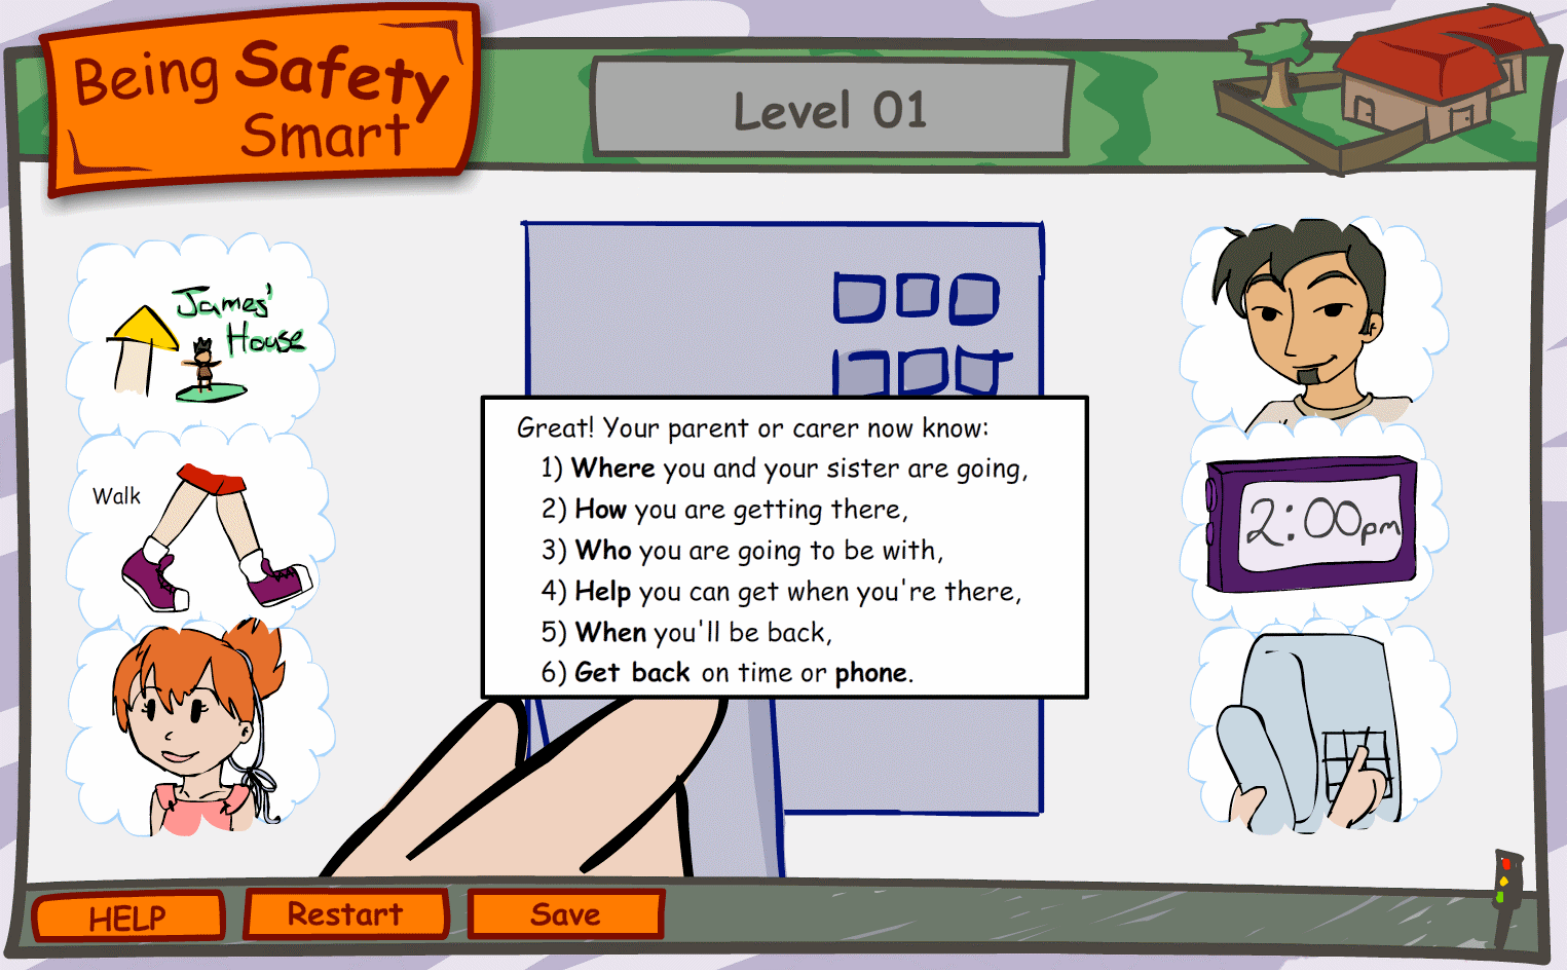
\includegraphics[width=\linewidth]{./Visuais/BSS/B5.png}}\vspace{-3pt}
  \\
  \subfloat[Nível 2\label{fig:2}\vspace{-5pt}]{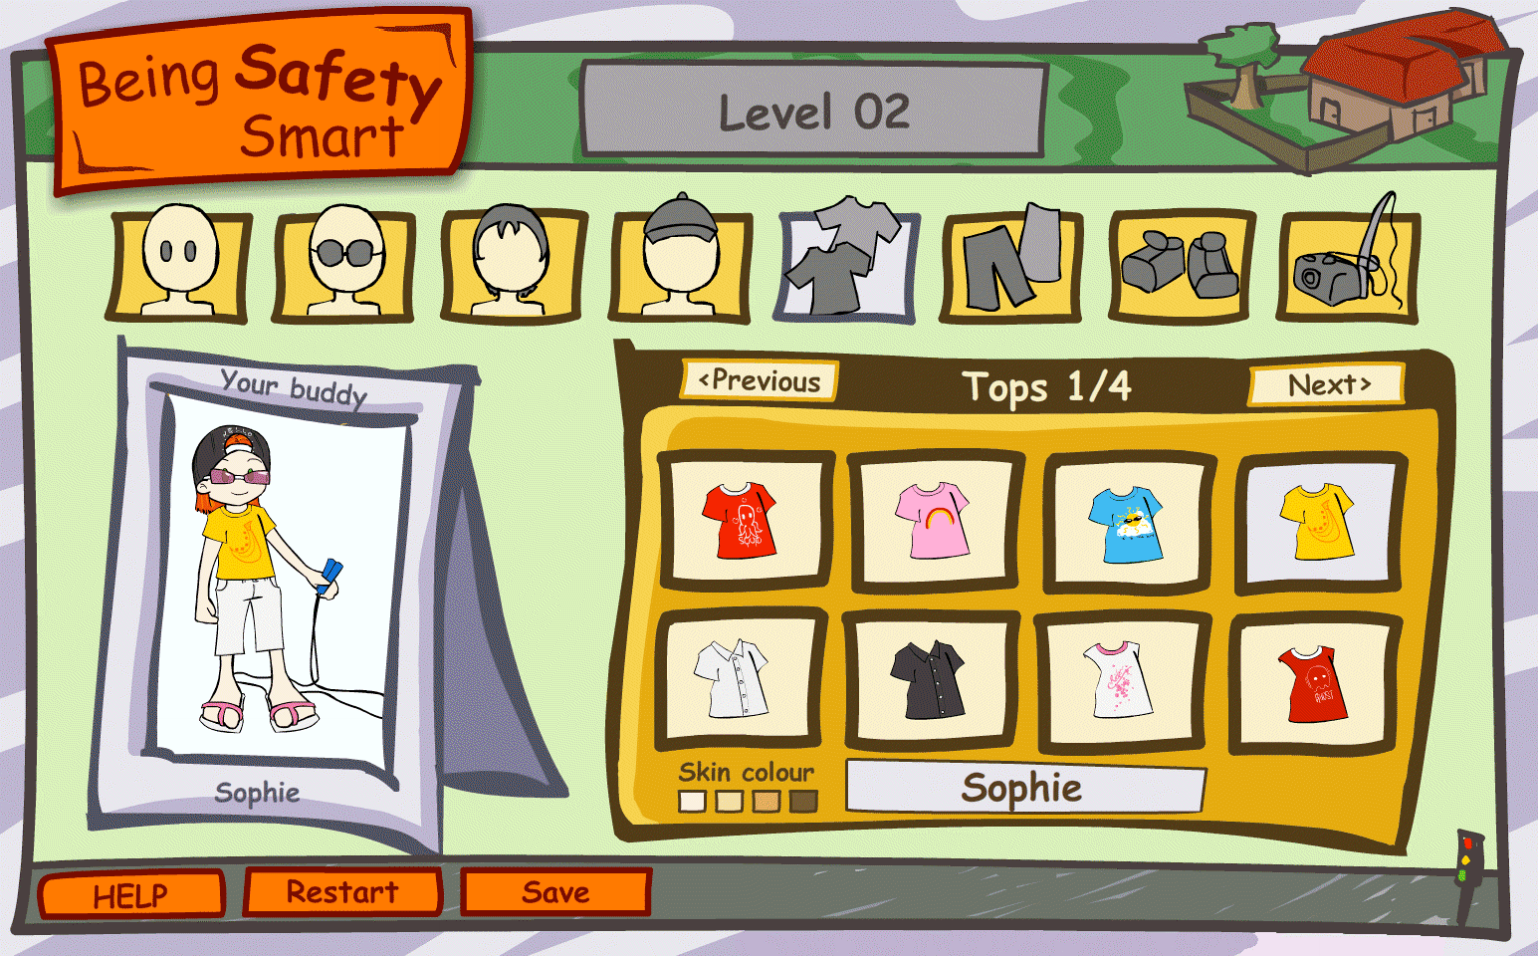
\includegraphics[width=\linewidth]{./Visuais/BSS/B2.png}}\vspace{-3pt}
  \\
  \subfloat[Nível 3\label{fig:3}\vspace{-5pt}]{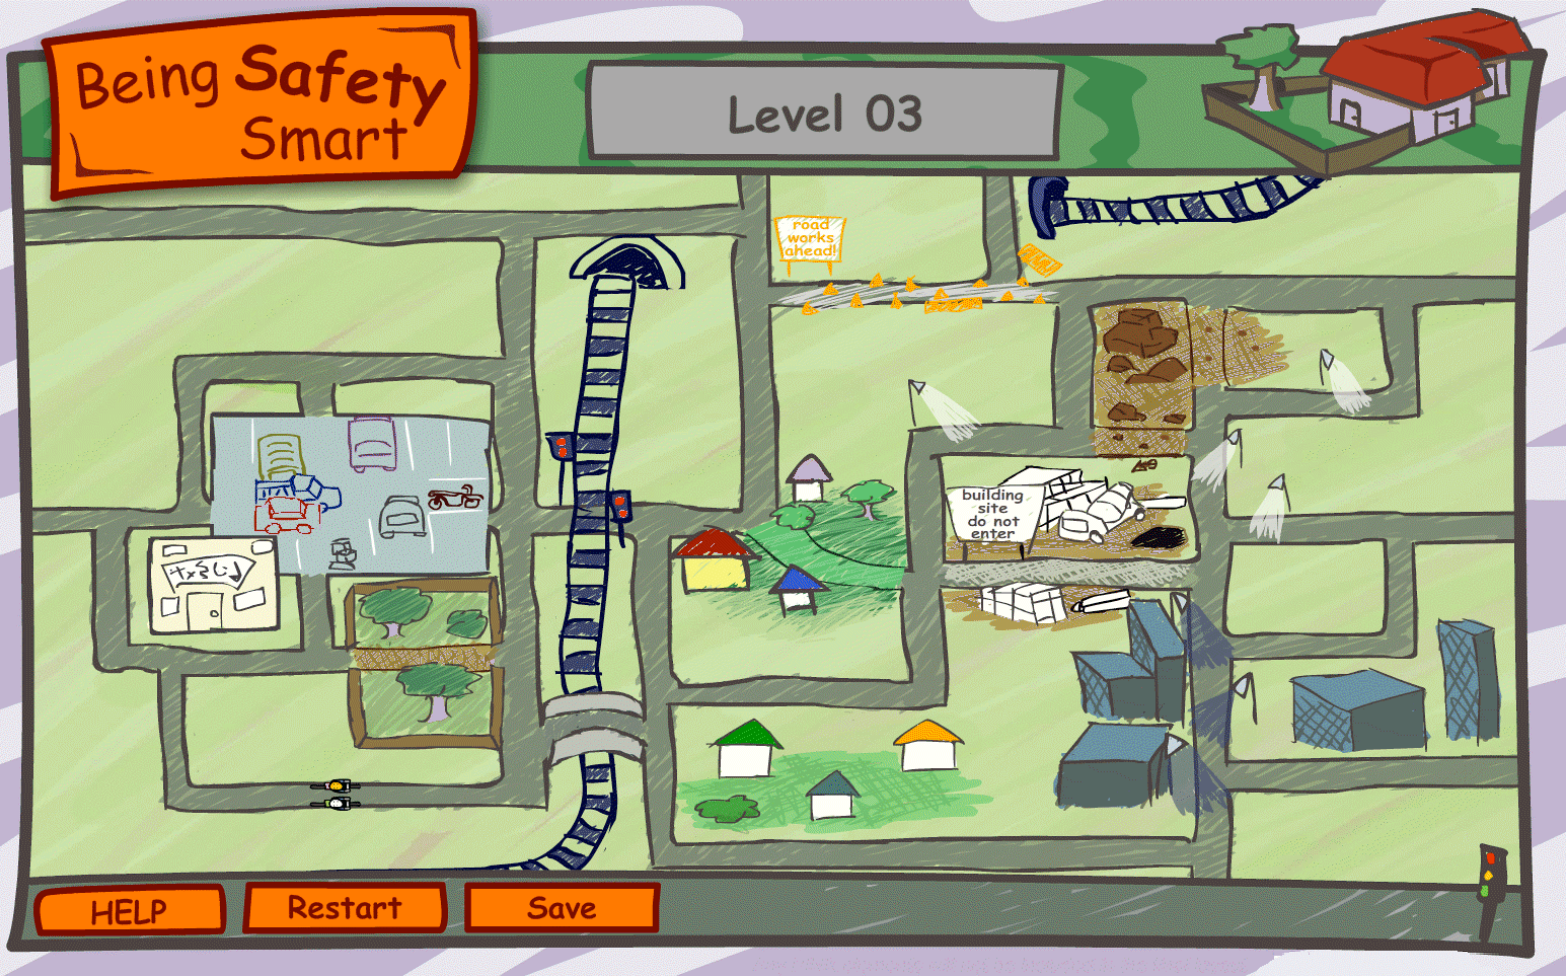
\includegraphics[width=\linewidth]{./Visuais/BSS/B8.png}}\vspace{-3pt}
  \\
  \subfloat[Nível 4\label{fig:4}\vspace{-5pt}]{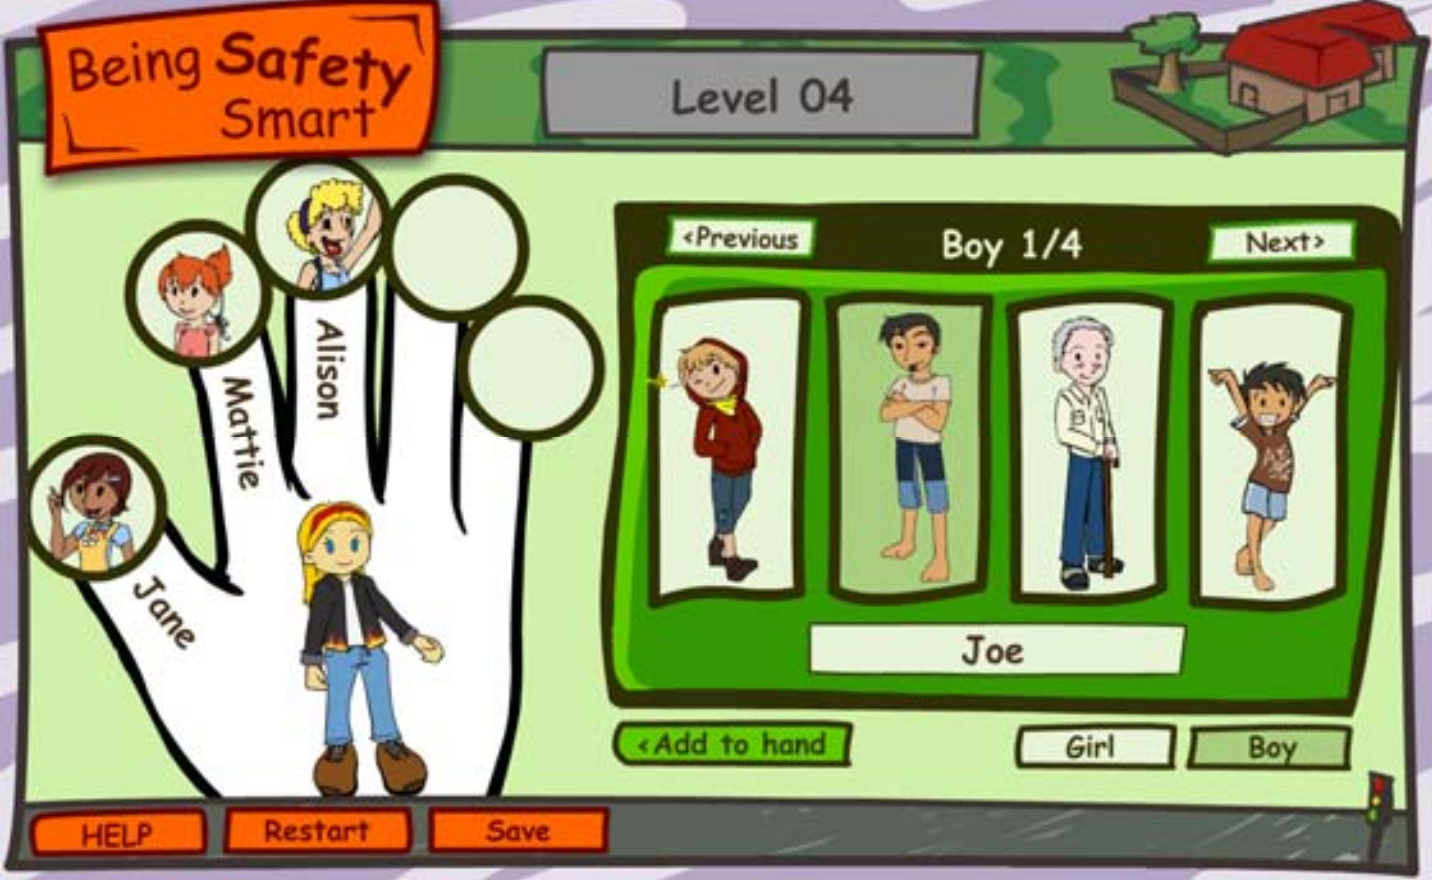
\includegraphics[width=\linewidth]{./Visuais/BSS/B9.png}}\vspace{-3pt}
  \\
  \subfloat[Nível 5\label{fig:5}\vspace{-5pt}]{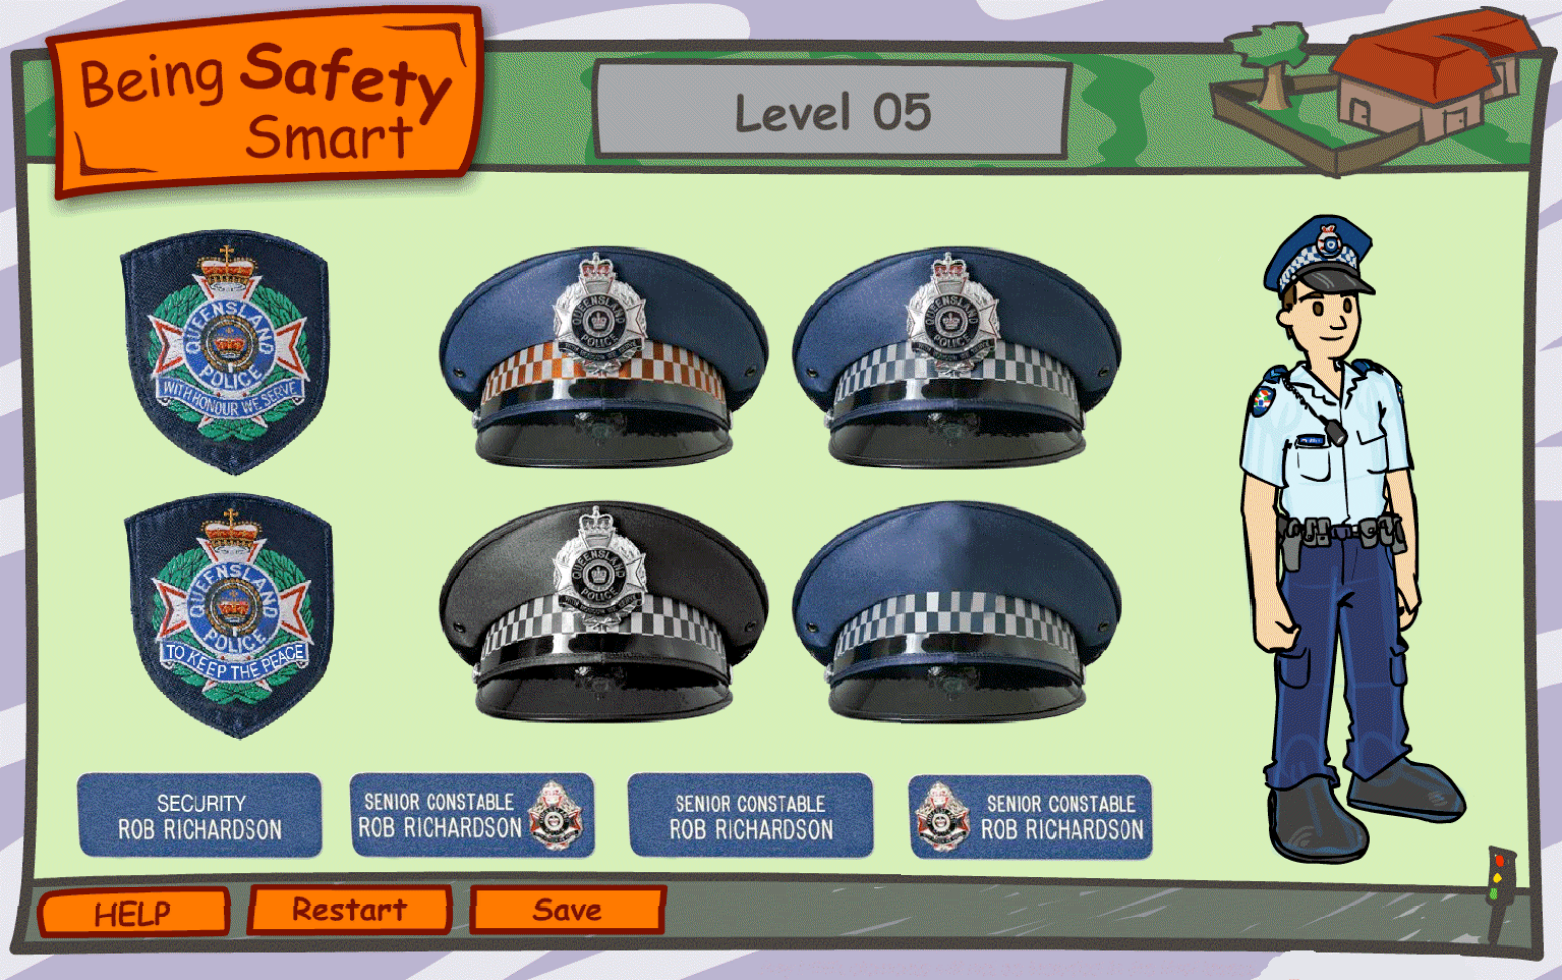
\includegraphics[width=\linewidth]{./Visuais/BSS/B6.png}}\vspace{-3pt}
  \\
  \subfloat[Nível 6\label{fig:6}\vspace{-5pt}]{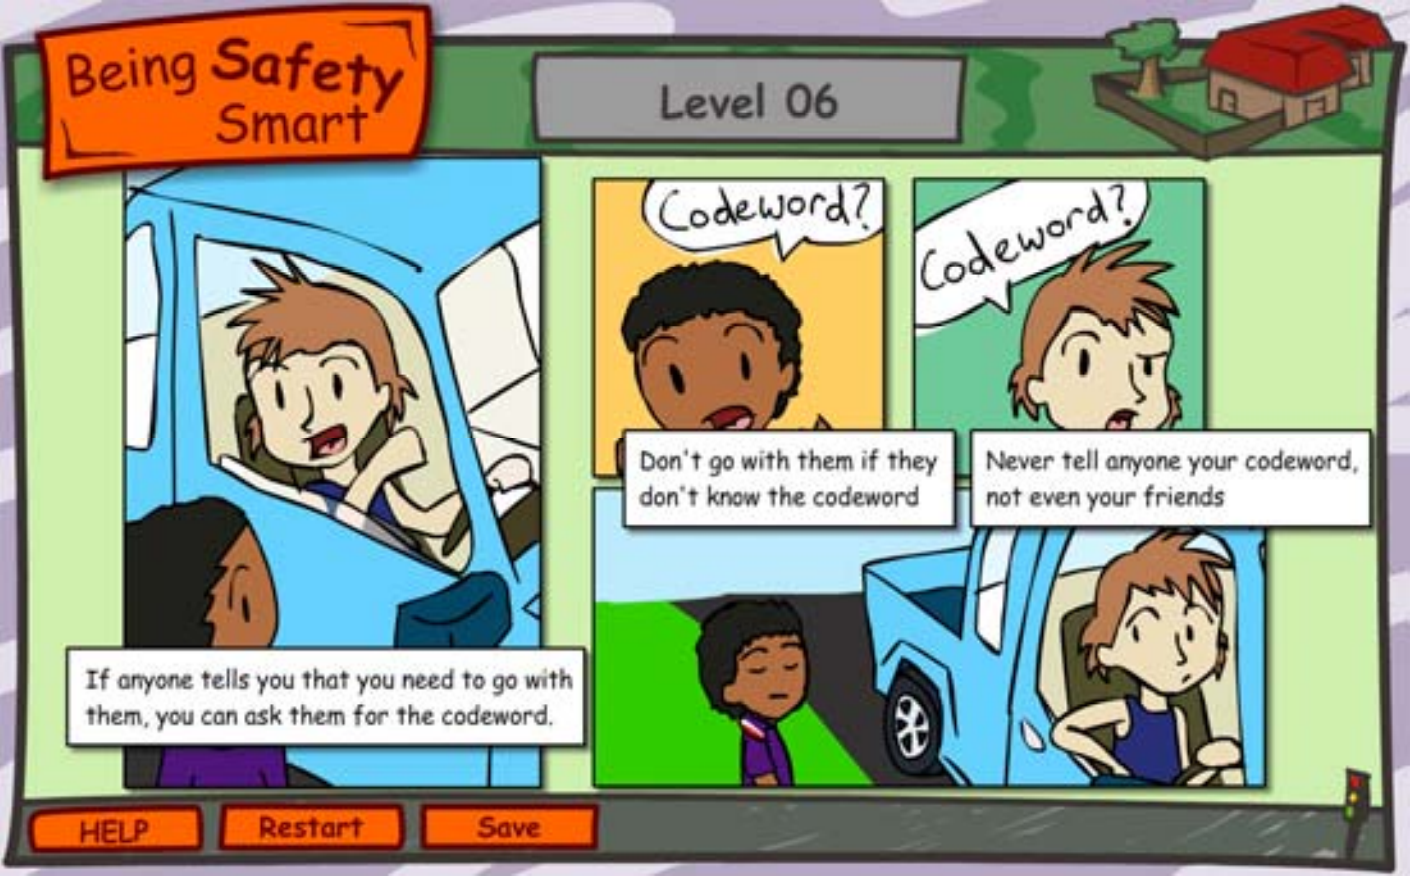
\includegraphics[width=\linewidth]{./Visuais/BSS/B10.png}}\vspace{-3pt}
  \\
  \subfloat[Nível 7\label{fig:7}\vspace{-5pt}]{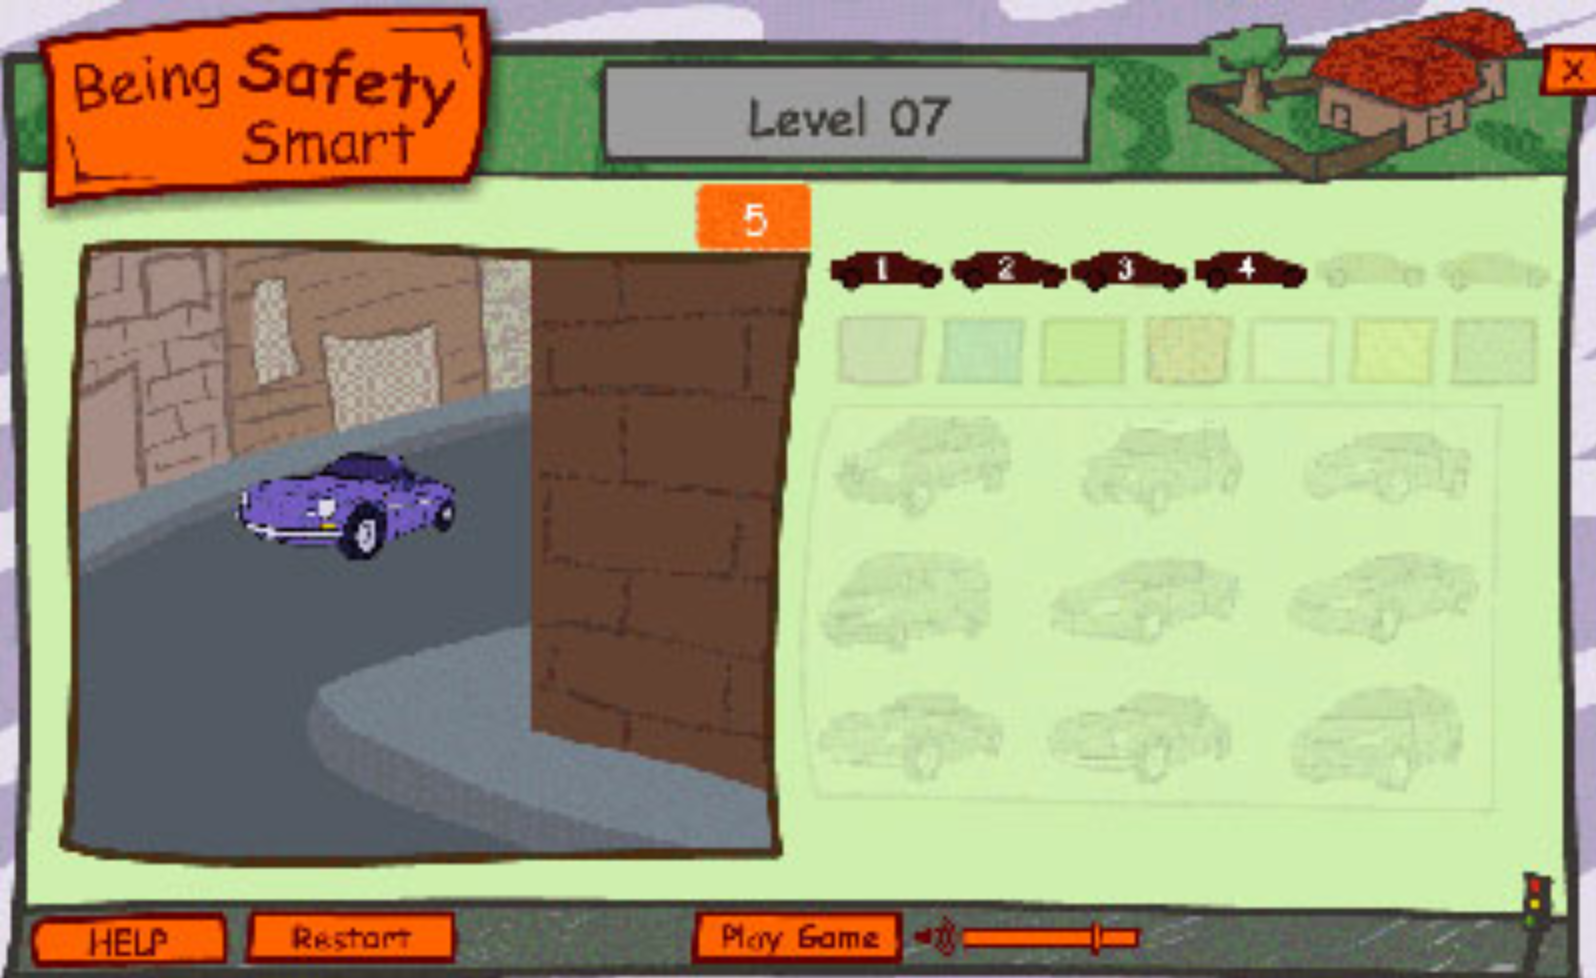
\includegraphics[width=\linewidth]{./Visuais/BSS/B12.png}}\vspace{-3pt}
  \\
  \subfloat[Nível 8\label{fig:8}\vspace{-5pt}]{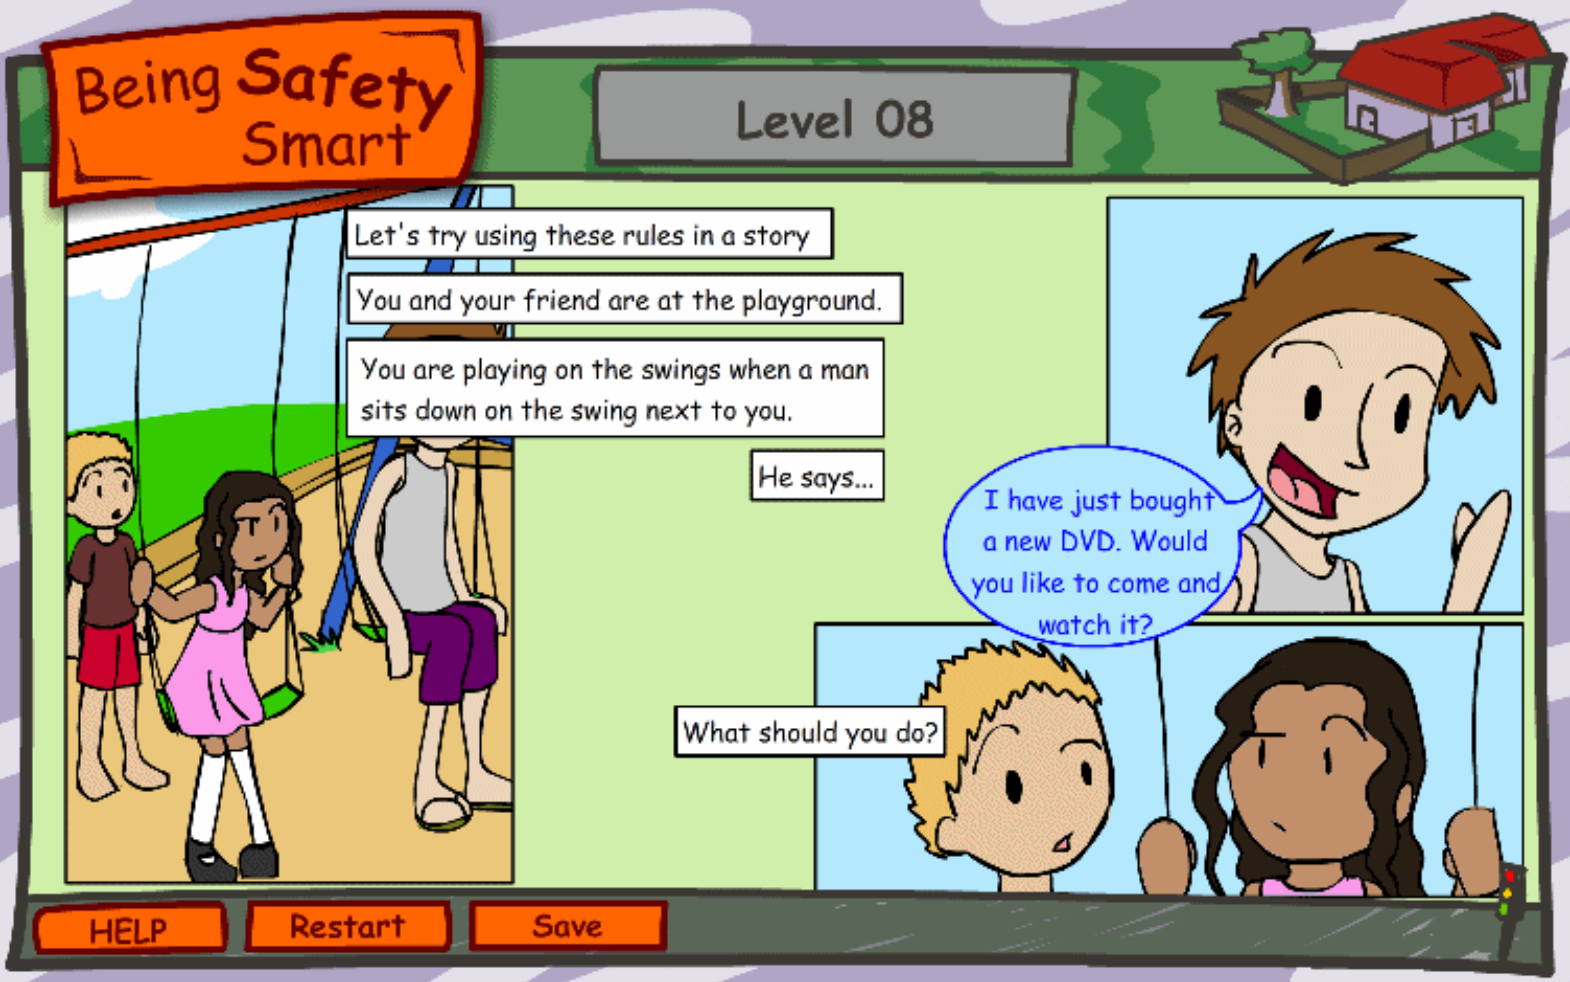
\includegraphics[width=\linewidth]{./Visuais/BSS/B11.png}}
  \vspace{-1pt}
  \legend{Fonte: \citeonline{jones2008online}.}%eu paguei outros nao citados aqui, como fazer a referencia?
  %india (mas não governamental)
\end{wrapfigure}

A numeração dos níveis representa a linearidade imposta pelo jogo ao jogador. O jogo exige um cumprimento linear dos seus níveis, tanto por motivos de enredo, quanto por motivos pedagógicos de ensino. Um jogador só pode acessar os níveis inferiores ao seu progresso no jogo. O jogador precisa esperar que a história do jogo vá destravando, um a um, os níveis superiores. Ao acessar o jogo, o jogador deve realizar um breve cadastro para ter acesso ao mapa do jogo e seus oito níveis, podendo ainda customizar seu personagem. No primeiro nível (Figura \ref{fig:1}) a criança aprende que deve sempre informar aos seus pais (ou responsáveis) os locais aonde vai e com quem vai ao sair de casa com os amigos. No segundo nível (Figura \ref{fig:2}) o jogador é ensinado a nunca andar sozinho sempre que isso for possível. No terceiro nível (Figura \ref{fig:3}) a criança é instruída a caminhar sempre por locais seguros e conhecidos. No quarto nível (Figura \ref{fig:4}) o menor aprende a reconhecer e identificar cinco adultos em quem possa confiar. No quinto nível (Figura \ref{fig:5}) o jogador é ensinado a identificar outras pessoas a quem possa pedir ajuda ou auxílio. No sexto nível (Figura \ref{fig:6}) o menor aprende a identificar pessoas confiáveis através de um sistema de contrassenha (\textit{e.g.} as contrassenhas ou \textit{codeworks} são senhas usadas entre as pessoas para reconhecerem se a outra pessoa é uma pessoa de confiança). No sétimo nível (Figura \ref{fig:7}) o jogador aprende a evitar presentes de estranhos (\textit{e.g.} evitando caronas de desconhecidos e presentes ou doces de estranhos). E no oitavo nível (Figura \ref{fig:8}) o jogo ensina ao jogador a sempre comunicar e contar para pessoas de confiança situações incomuns ou desagradáveis que tenham acontecido. 

Todos os níveis do jogo \textit{Being Safety Smart} compartilham a mesma arte baseada em quadrinhos infantis. Cada diálogo do jogo é acompanhado por texto escrito e dublagem em língua inglesa. Além disso, os níveis do jogo compartilham a mesma estrutura didática baseada em três conceitos metodológicos de ensino. Inicialmente o jogador é apresentado as instruções de um determinado nível. Posteriormente o jogador é confrontado com uma atividade lúdica interativa. E por fim, o jogador é apresentado a um resumo do nível. Os oito níveis do jogo são projetados para serem ministrados em um ambiente escolar no decorrer de 8 (oito) semanas. Contudo, nada impede que o jogo seja ofertado em blocos mais curtos ou mais longos de tempo a depender das temáticas já ministradas pela escola \cite{jones2010being}. Em adendo, a literatura revela que mais de 200 (duzentas) escolas já ministraram o jogo \textit{Being Safety Smart} a seus alunos.

O jogo \textit{Being Safety Smart} teve sua eficácia verificada por meio de um processo avaliativo \cite{jones2010being}. O processo buscou encontrar relações entre os graus de aprendizagem de uma amostra de crianças e os assuntos ministrados pelo jogo. Para se verificar essa relação, a amostra de crianças foi previamente dividida em dois grupos: um grupo controle e um grupo experimental. O grupo controle consistia do conjunto de participantes (crianças) que não jogaram o jogo. O grupo experimental, por sua vez, consistia do conjunto de participantes (crianças) que jogaram o jogo \textit{Being Safety Smart}. O processo avaliativo mediu então, os graus de aprendizagem dos participantes anteriormente (pré-teste) e posteriormente (pós-teste) aos testes com o jogo. A medicação dos graus de aprendizagem dos participantes se deu por meio do questionário \acf{CKAQ}. A ideia da etapa de pré-teste é averiguar o alinhamento no nível de conhecimento de ambos os grupos no que diz respeito aos conteúdos do questionário. Já a ideia da etapa de pós-teste é constatar diferenças significativas no nível de conhecimento entre os grupos no que diz respeito também, aos conteúdos do questionário.

A etapa da pré-teste teve a participação de 70 (setenta) crianças: 34 (trinta e quatro) do grupo controle e 36 (trinta e seis) do grupo experimental. A medição dos resultados revelou uma taxa de acerto do questionário de 67,83\% ($\sigma$ = 7,91\%) para o grupo controle e 66,11\% ($\sigma$ = 15,41\%) para o grupo experimental. Os resultados demonstram que ambos os grupos compartilhavam o mesmo nível de conhecimento na etapa de pré-teste da pesquisa \cite{jones2010being}. Após estes resultados, o grupo experimental foi convidado a jogar o jogo. Depois de jogar o jogo por 8 (oito) semanas, ambos os grupos foram convidados a responderem novamente o questionário \ac{CKAQ}. 

A etapa de pós-teste teve a participação de 76 (setenta e seis) crianças: 37 (trinta e sete) do grupo controle e 39 (trinta e nove) do grupo experimental. A medição dos resultados apresentou um percentual de acerto do questionário de 69,11\% ($\sigma$ = 10,49\%) para o grupo controle e 89,97\% ($\sigma$ = 11,18\%) para o grupo experimental. Os dados mostram uma nítida evolução no desempenho do grupo experimental em relação ao grupo controle, implicando assim, uma possível influência do jogo ministrado. Entre os jogadores, o jogo parece ser capaz de ampliar a compreensão das crianças no que diz respeito as estratégias de segurança pessoal.

Durante toda a pesquisa os profissionais envolvidos receberam treinamento adequado, sendo instruídos a proceder adequadamente a quaisquer casos de violência sexual infantil que fossem revelados no decorrer da pesquisa \cite{jones2010being}. Além disso, os responsáveis das crianças tiveram participação ativa neste processo, sendo responsáveis por notificarem qualquer alteração no comportamento das crianças como ansiedade ou angústia. O jogo então manifesta dois resultados positivos, o primeiro de ampliar os conhecimentos das crianças acerca sua segurança pessoal e o segundo pelo fato do jogo não manifestar qualquer desconforto ou mudança inadequada de comportamento aos jogadores. 

%-------------------------------------------------------------------------------------------------------------------

\section{Orbit Rescue}\label{sssec:Orbit}

\textit{Orbit Rescue}\footnote{\textit{Orbit Rescue} é um jogo sério desenvolvido pela Universidade de Sunshine Coast e lançado em 2012. Mais informações sobre o jogo podem ser acessadas em seu portal: \url{http://orbit.org.au/}.} é um jogo no estilo aventura projetado para conscientizar as crianças sobre a violência sexual infantil. O jogo é voltado a atender crianças entre 8 (oito) e 10 (dez) anos de idade. Dentre os ensinamentos ministrados pelo jogo estão conceitos de: privacidade corporal, comunicação, confiança e defesa pessoal. Os quatro ensinamentos se traduzem em quatro fases a serem acessadas no jogo, o qual possui texto e dublagem em inglês, apenas. A \autoref{fig:selecao} ilustra a tela de seleção de fases do jogo.

\begin{figure}[htb]
	\caption{\label{fig:selecao}Tela de seleção das fases do jogo \textit{Orbit Rescue}.}
  \begin{center}\vspace{-0.3cm}
    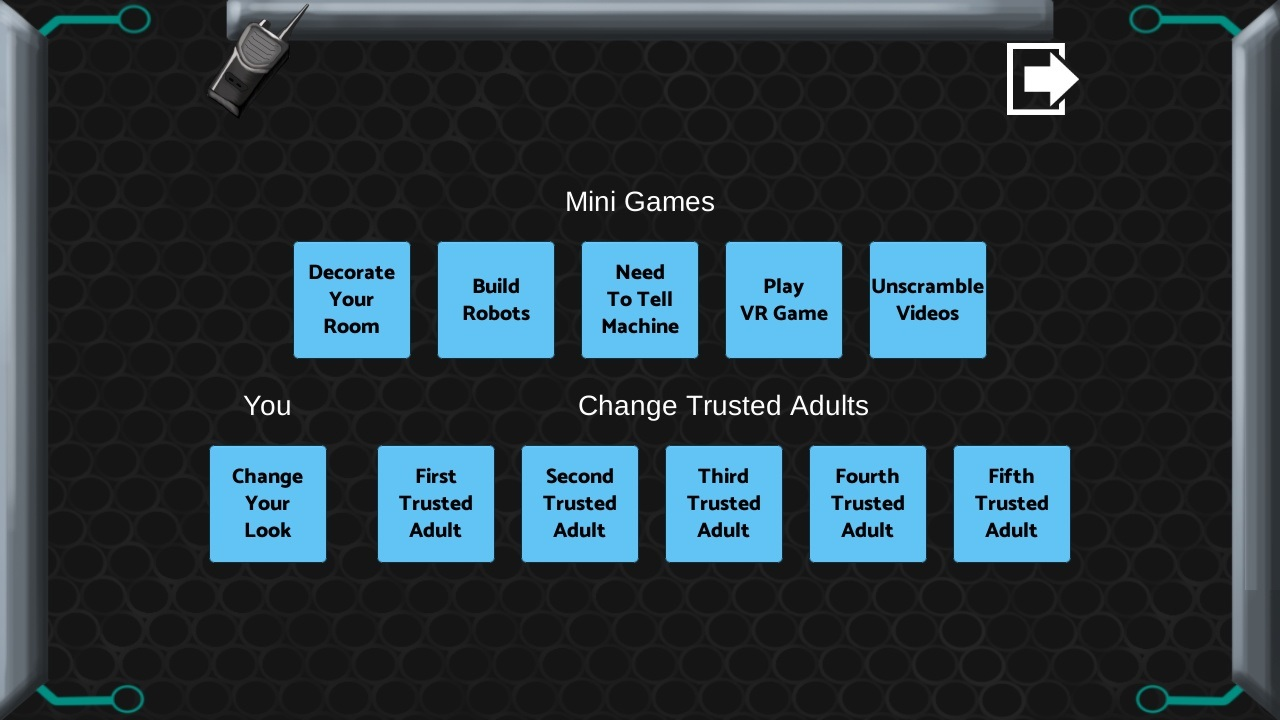
\includegraphics[width=0.92\linewidth]{./Visuais/Orbit/OrbitFases.jpg}
	\end{center}\vspace{-0.2cm}
  \legend{Fonte: \citeonline{steiler2012orbit}}
\end{figure}

\vspace{-0.3cm}


O jogo \textit{Orbit Rescue} dispõe de dois canais de acesso as fases do jogo. As fases do jogo podem ser acessadas em determinados cenários, ou podem ser acessadas por meio de um ícone que leva a uma tela de seleção de fases como mostra a \autoref{fig:selecao}. Cada fase se traduz em um minijogo com dinâmica e ensinamentos distintos entre si, cada fase contém uma quantidade variadas de níveis a serem explorados. Há ainda conceitos não ministrados nos minijogos, com a questão dos adultos de confiança. Tal conceito é passado com o intuito de ensinar ao jogador a reconhecer e identificar pessoas em quem possa confiar. O jogador deve então, personificar no jogo cinco adultos de confiança. Indiretamente o jogador aprende a sempre estar acompanhado por alguém de confiança, pois o personagem fabricado acompanha o personagem do jogador em grande parte da história do jogo. Por fim, a \autoref{fig:selecao} também apresenta algumas opções que não estão associados a um contexto pedagógico direto, como a customização do personagem ou do quarto do personagem. Por não terem significância didática, tais opções não são apresentadas nesse trabalho. 


\begin{wrapfigure}[30]{r}{5.5cm}%pulando 30 linhas
  \vspace{-5pt}
  \caption{\label{fig:orbitniveis}Níveis.\vspace{0pt}}

  \subfloat[Nível 1\label{fig:11}\vspace{-2pt}]{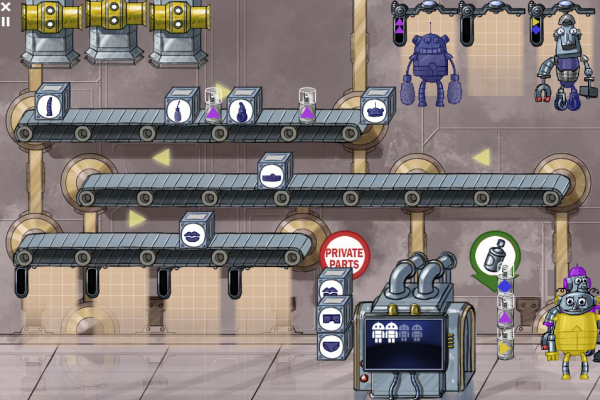
\includegraphics[width=\linewidth]{./Visuais/Orbit/robot-factory-screenshot.png}}\vspace{-0pt}
  \\
  \subfloat[Nível 2\label{fig:22}\vspace{-2pt}]{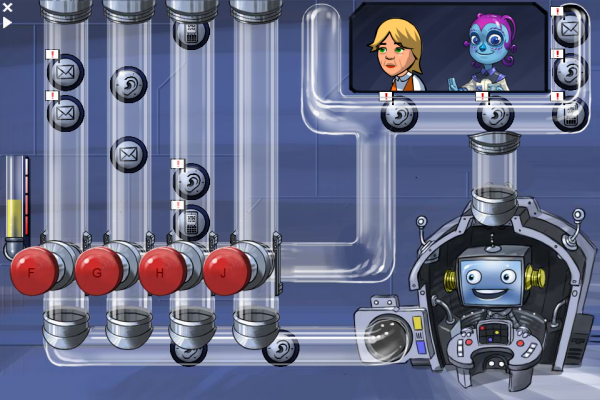
\includegraphics[width=\linewidth]{./Visuais/Orbit/need-to-tell.png}}\vspace{-0pt}
  \\
  \subfloat[Nível 3\label{fig:33}\vspace{-2pt}]{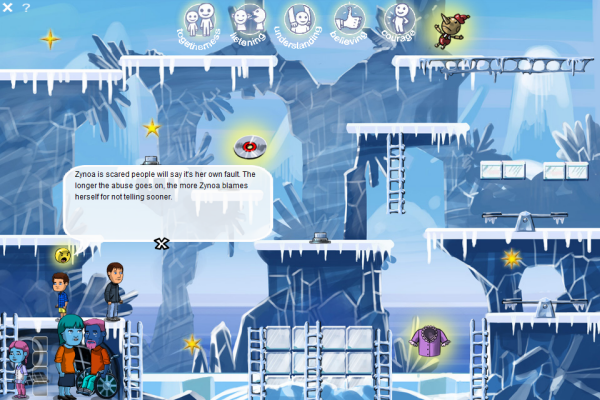
\includegraphics[width=\linewidth]{./Visuais/Orbit/speak-up.png}}\vspace{-0pt}
  \\
  \subfloat[Nível 4\label{fig:44}\vspace{-2pt}]{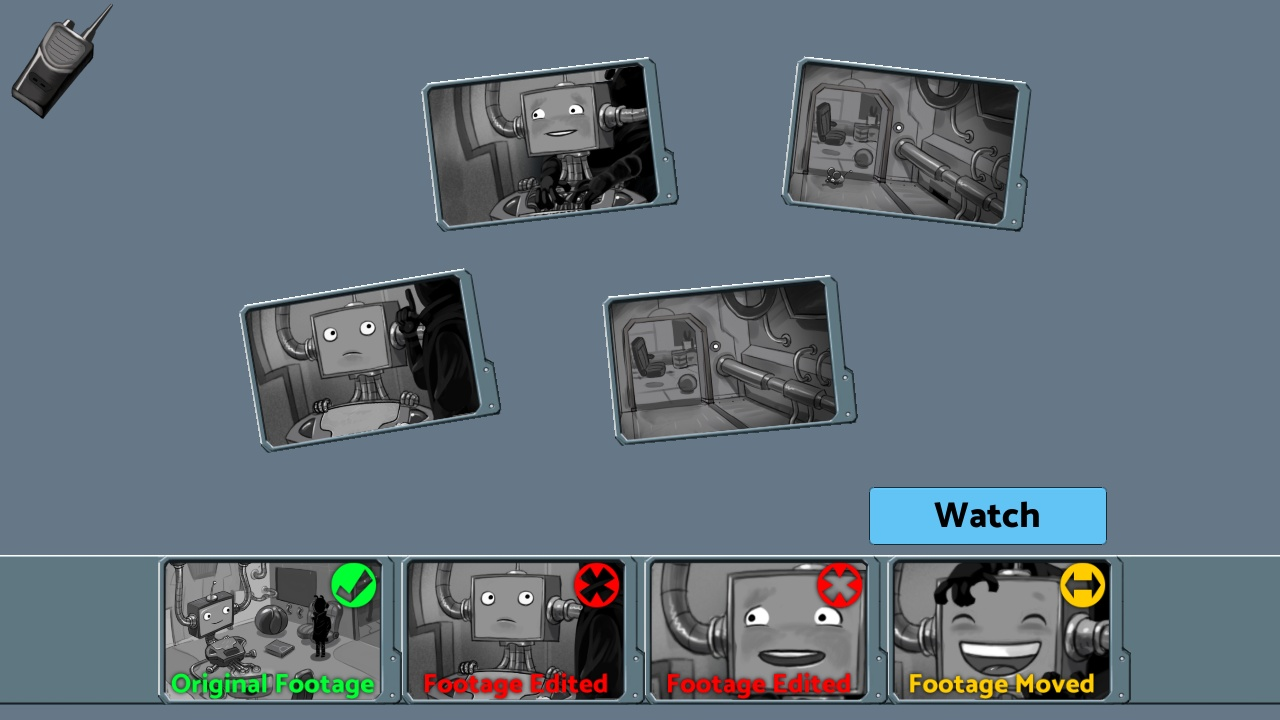
\includegraphics[width=\linewidth]{./Visuais/Orbit/cameras.jpg}}\vspace{-0pt}
  \vspace{-2pt}
  \legend{Fonte: \citeonline{steiler2012orbit}}%eu paguei outros nao citados aqui, como fazer a referencia?
  %india (mas não governamental)
\end{wrapfigure}

A \autoref{fig:orbitniveis} apresenta os quatro minijogos ministrados pelo jogo \textit{Orbit Rescue}. Cabe salientar que o jogo segue uma narrativa, por tal razão as fases não se encontram disponíveis ao jogador em um momento inicial. A ordem estabelecida na \autoref{fig:orbitniveis} representa a ordem que as fases vão sendo liberadas ao jogador. Inicialmente o jogador é ensinado sobre sua privacidade corporal (Figura \ref{fig:11}), nesta fase o jogador aprende quais são as partes íntimas e que elas não devem ser tocadas. Em seguida o jogador é ensinado a se comunicar devidamente (Figura \ref{fig:22}), o intuito desta fase é ajudar a criança a identificar situações que precisam ser reportadas para adultos de confiança. Conforme a história do jogo avança a criança aprende em um dado momento a ganhar confiança (Figura \ref{fig:33}), essa fase almeja ensinar a criança a superar episódios de abuso e a como proceder em tais situações. Por fim, em sua última fase, o jogo discorre sobre as abordagens utilizadas pelos agressores sexuais  (Figura \ref{fig:44}), o jogador então deve identificar neste momento como é a atuação de um agressor sexual e aprender a reconhecer tais estratégias desde seu momento inicial e a tomar as devidas medidas. A conclusão da última fase encerra a história e a narrativa do jogo. Salienta-se nesse sentido que, embora os minijogos acompanhem o enredo do jogo, o jogador é livre para acessar qualquer uma das fases já liberadas sempre que desejar, sem quaisquer prejuízos a narrativa ou a história do jogo. 

O jogo \textit{Orbit Rescue} passou por um processo avaliativo com o intuito de averiguar o conhecimento dos jogadores sobre o abuso infantil. Para averiguar o conhecimento dos jogadores os pesquisadores utilizaram o questionário \ac{CKAQ} nas etapas de pré e pós-teste da pesquisa \cite{jones2020serious}.

O processo avaliativo durou cerca de 4 (quatro) meses. Ao total 139 (cento e trinta e nove) crianças dispersas em três grupos participaram da pesquisa. O primeiro grupo foi submetido ao jogo e a um plano de ensino. O segundo grupo foi submetido apenas ao jogo. E o terceiro grupo não foi submetido nem ao jogo nem ao plano de ensino. Na etapa de pré-teste todos os grupos beiraram uma taxa de acerto de 75\% no questionário. O mesmo resultado se manteve para o terceiro grupo na etapa de pós-teste, porém o primeiro e o segundo grupo alcançaram uma taxa de acerto no questionário de 90\%. Salienta-se que o primeiro grupo acertou em média, uma ou duas questões a mais no questionário em relação ao segundo grupo. A análise dos resultados revela a eficácia do jogo no que diz respeito aos conteúdos ministrados.

%Olhando individualmente, as crianças que mais obtiveram mais sucesso no questionário foram as que finalizaram o jogo, evidenciando assim, os sucesso do jogo na temática tratada.

%-------------------------------------------------------------------------------------------------------------------

\section{Cool and Safe}\label{sssec:CeS}

\textit{Cool and Safe}\footnote{\textit{Cool and Safe} é um jogo desenvolvido pela Universidade de Frankfurt lançado ao público em 2013. Mais informações sobre o jogo podem ser acessadas em seu portal: \url{https://www.coolandsafe.eu/}.} é um jogo para navegadores voltado para prevenção da violência sexual de crianças. O jogo é destinado a atender crianças na faixa dos 7 (sete) aos 12 (doze) anos. O jogo almeja prevenir a violência sexual infantil por meio da expansão do repertório comportamental das crianças, do fortalecimento de suas habilidades de autoafirmação e por meio de instruções para as crianças aprenderem a lidar com situações perigosas \cite{pajala2018compiled}. O jogo está inteiramente localizado em alemão e em francês. Todos os assuntos ministrados pelo jogo, são transmitidos as crianças por meio de texto, imagem ou vídeo em alemão ou em francês, a depender das configurações de idioma. A página inicial do portal do jogo é mostrada na \autoref{fig:portal}.

\begin{figure}[htb]

	\caption{\label{fig:portal}Portal do jogo \textit{Cool and Safe}.}
  \begin{center}%\vspace{-0.3cm}
    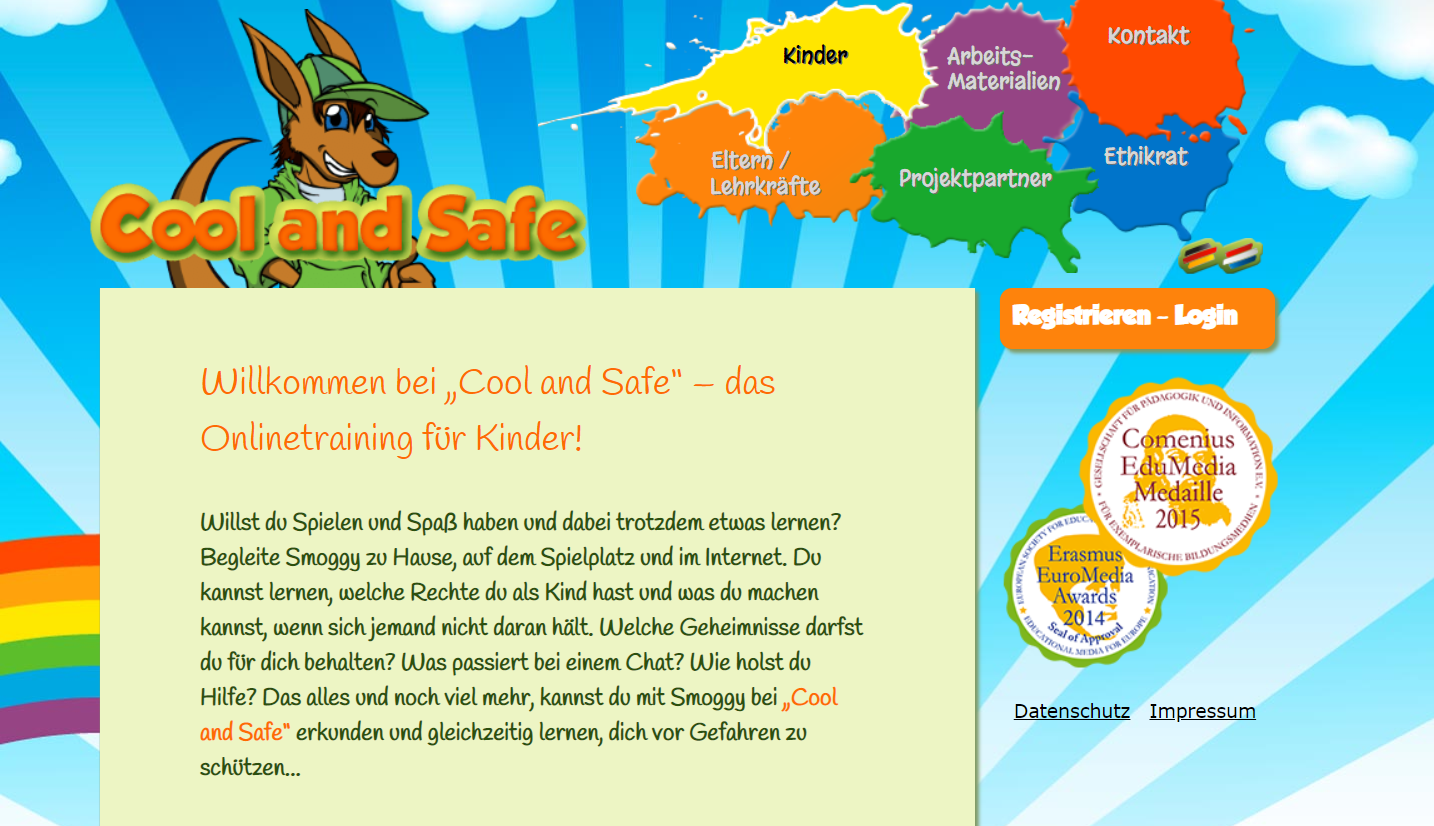
\includegraphics[width=\linewidth]{./Visuais/Cool/coolSafe.png}
	\end{center}%\vspace{-0.5cm}
  \legend{Fonte: \citeonline{fingerle2012cool}}

\end{figure}

A \autoref{fig:portal} apresenta a página principal do portal do jogo \textit{Cool and Safe}. Nesta página é possível observar as opções para troca de idioma, simbolizadas pelas bandeiras da França e da Alemanha. O jogo requer um cadastro para acesso, sendo necessário cadastrar um nome, senha, dia e mês de aniversário. Após o cadastro, o jogador obtém livre acesso ao jogo. Ao começar a jogar, o jogador é apresentado a vários clipes de filmes, histórias e tarefas nos quais deve ponderar e escolher entre diferentes alternativas \cite{mueller2012web}. 

\begin{wrapfigure}[30]{r}{5.5cm}%pulando 30 linhas
  \vspace{-5pt}
  \caption{\label{fig:coolniveis}Níveis.\vspace{1pt}}

  \subfloat[Nível 1\label{fig:111}\vspace{-7pt}]{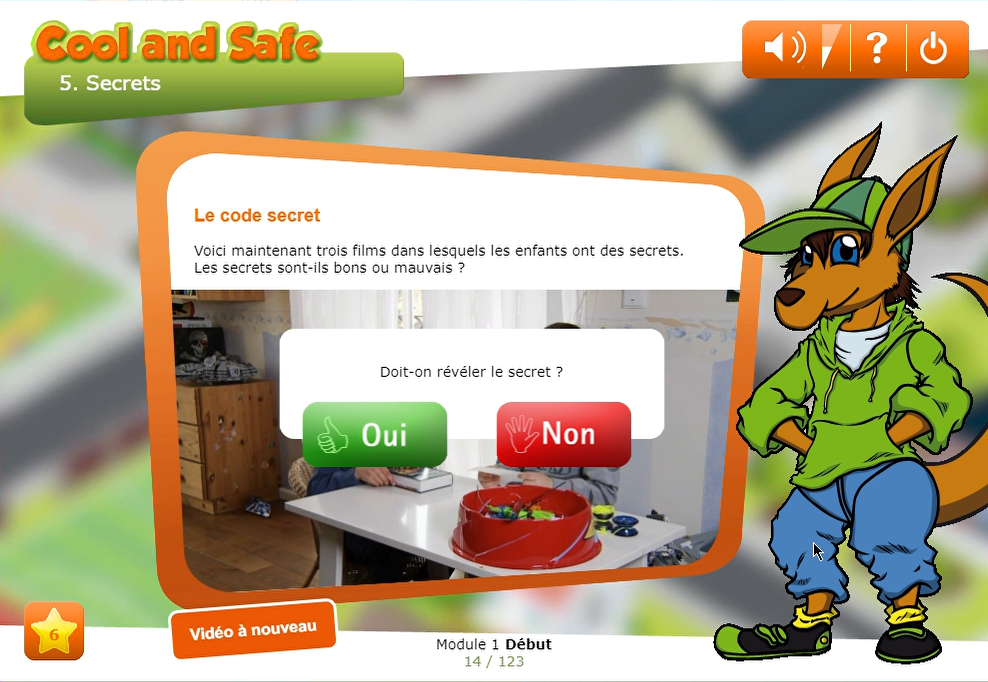
\includegraphics[width=\linewidth]{./Visuais/Cool/nivel11.png}}\vspace{-2pt}
  \\
  \subfloat[Nível 2\label{fig:222}\vspace{-7pt}]{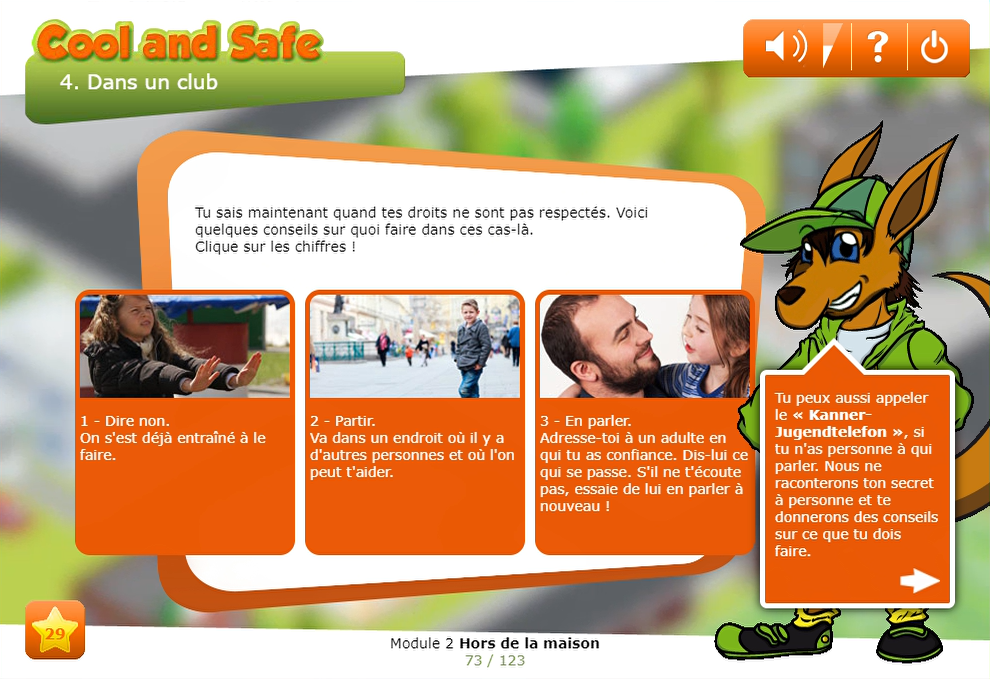
\includegraphics[width=\linewidth]{./Visuais/Cool/nivel222.png}}\vspace{-2pt}
  \\
  \subfloat[Nível 3\label{fig:333}\vspace{-7pt}]{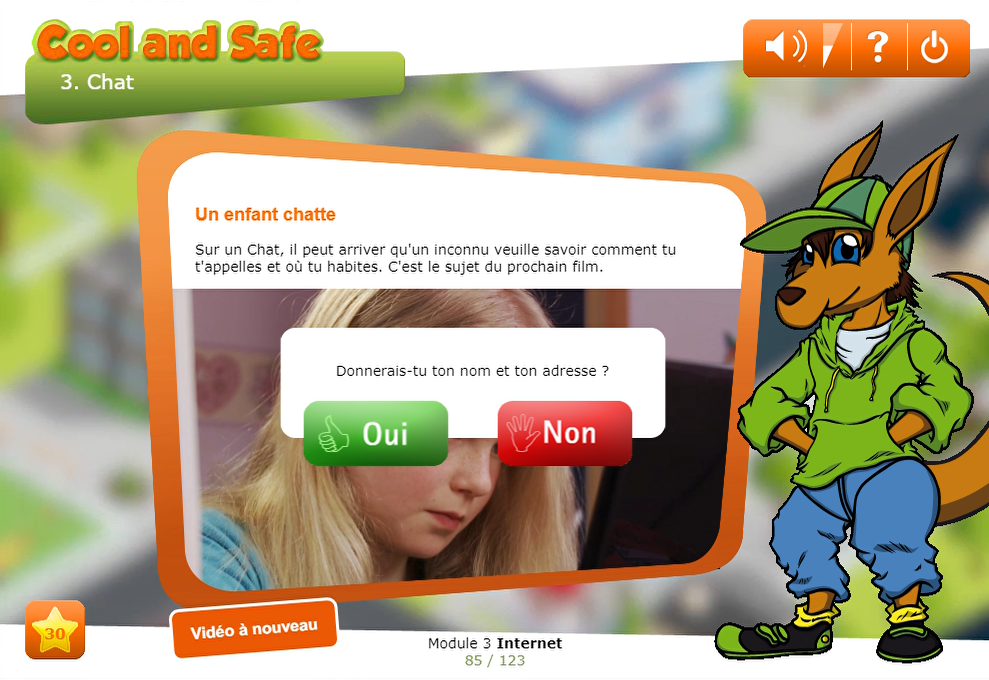
\includegraphics[width=\linewidth]{./Visuais/Cool/nivel3.png}}\vspace{-2pt}
  \\
  \subfloat[Nível 4\label{fig:444}\vspace{-7pt}]{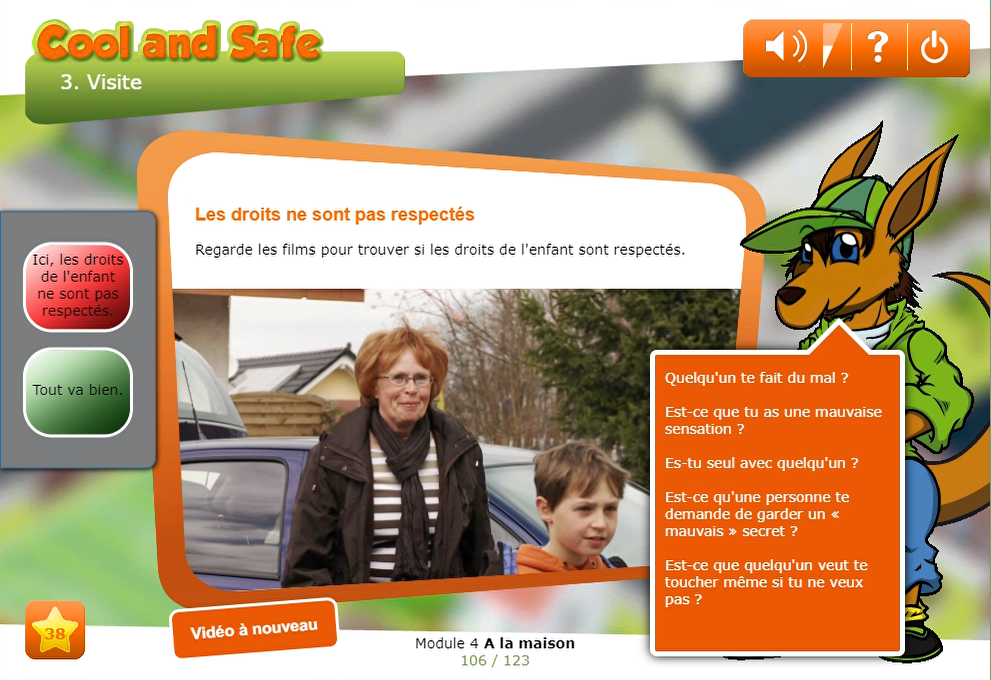
\includegraphics[width=\linewidth]{./Visuais/Cool/nivel4.png}}\vspace{-2pt}
  \vspace{-2pt}
  \legend{Fonte: \citeonline{fingerle2012abschlussbericht}}%eu paguei outros nao citados aqui, como fazer a referencia?
  %india (mas não governamental)
\end{wrapfigure}

O jogo é constituído por cinco módulos de ensinamentos para as crianças. Cada módulo corresponde a um conceito distinto a ser apreendido pelo jogador. A sequência dos módulos é fixa e não pode ser alterada. Portanto, não é possível realizar módulos individuais separadamente, além disso o jogador não possui flexibilidade para retornar para um determinado módulo após concluí-lo. O primeiro módulo (Figura \ref{fig:111}) consiste em apresentar alguns conceitos básicos ao jogador como interpretar sentimentos, guardar ou não segredos e conversar com os pais. O segundo módulo (Figura \ref{fig:222}) consiste em um tópico mais avançado voltado a educar sobre situações que podem ocorrer fora de casa como aceitar doces de estranhos, identificar situações perigosas e recusar caronas de estranhos. O terceiro módulo (Figura \ref{fig:333}) é destinado a ensinar ao jogador como usar adequadamente a \textit{internet}, neste módulo o jogador é ensinado a usar adequadamente as redes sociais, não adicionar estranhos e não ceder suas informações pessoais para terceiros. O quarto módulo (Figura \ref{fig:444}) busca educar o jogador sobre situações que podem acontecer dentro de casa, aqui a criança é ensinada sobre seus direitos e deveres, ensinada a não abrir a porta para estranhos e ensinada a denunciar a quebra de seus direitos para outras pessoas. O último módulo (sem figura representativa) apresenta uma compilação de algumas lições aprendidas nos módulos anteriores servindo como uma espécie de revisão. 

O jogo \textit{Cool and Safe} passou por um processo avaliativo, com intuito de identificar possíveis efeitos colaterais negativos relacionado à conclusão do jogo e sua eficácia. Ao total 286 (duzentas e oitenta e seis) crianças participaram do processo avaliativo \cite{muller2014child}. 

O processo avaliativo do jogo \textit{Cool and Safe} segmentou sua amostra de crianças em dois grupos: um grupo controle e um grupo experimental. Na etapa de pré-teste da pesquisa não se constatou diferença significativa entre os conhecimentos das crianças aos responderem o questionário \ac{CKAQ}, com ambos os grupos atingindo uma média de acerto no questionário de 61\% ($\sigma$ = 16\%). Este mesmo valor se manteve no grupo controle na etapa de pós-teste, contudo nesta etapa o grupo experimental alcançou uma taxa de 79\%  ($\sigma$ = 14\%) de acerto do questionário. Os dados provam a eficácia do jogo. Além disso, testes emocionais foram realizados, os quais não identificaram quaisquer efeitos colaterais negativos manifestados pelas crianças após a conclusão do jogo, demonstrando que seu conteúdo se encontra adequado a idade ministrada. 


%-------------------------------------------------------------------------------------------------------------------

\section{Análise Comparativa}\label{sssec:finais}

Os jogos elencados neste Capítulo são uma resposta ao problema da violência sexual de crianças e de adolescentes. O estudo de tais jogos permite tanto compreender suas estruturas didático-pedagógicas, quanto os processos envolvidos na validação de tais jogos. Neste sentido, observou-se que o questionário \acf{CKAQ} norteia o processo avaliativo dos jogos apresentados. É importante que diferentes pesquisas atestem seus resultados acadêmicos através da utilização das mesmas métricas, para que o rigor do processo científico seja preservado. Assim, os resultados e achados entre uma pesquisa e outra ficam mais evidentes, uma vez que todas tenham se utilizado da mesma régua. A \autoref{tab-nivinv} compila os principais achados científicos dos trabalhos relacionados a essa pesquisa.


\newcolumntype{P}[1]{>{\centering\arraybackslash}p{#1}}
\newcolumntype{M}[1]{>{\centering\arraybackslash}m{#1}}
\begin{table}[htb]
\footnotesize
\renewcommand{\arraystretch}{1.5} %espaço entre as linhas
\caption[Trabalhos Relacionados.]{Trabalhos Relacionados.}
\label{tab-nivinv}
\centering
\begin{tabular}{p{4.2cm}p{2.0cm}M{2.2cm}M{1.5cm}M{2.0cm}M{2.1cm}}
  \toprule
   \textbf{Jogo (Ano)} & \textbf{Idioma}  & \textbf{Público-alvo} & \textbf{Amostra} & \multicolumn{2}{c}{\textbf{Validação (pós-teste)}}  \\
   \cline{5-6}
     &  &  &  & Grupo Controle & Grupo Experimental\\
   \midrule
    \textit{Being Safety Smart} (2009)  & Inglês          & 6-8 anos    & 76    & \textcolor[rgb]{0.9,0,0}{\textbf{69\%}}      & \textcolor[rgb]{0,0.6,0}{\textbf{90\%}} \\
    \hline
    \textit{Orbit Rescue} (2012)        & Inglês          & 8-10 anos   & 139    & \textcolor[rgb]{0.9,0,0}{\textbf{75\%}}      & \textcolor[rgb]{0,0.6,0}{\textbf{93\%}} \\
    \hline
    \textit{Cool and Safe} (2013)       & Alemão/Francês  & 7-12 anos   & 286   & \textcolor[rgb]{0.9,0,0}{\textbf{61\%}}      & \textcolor[rgb]{0,0.6,0}{\textbf{79\%}} \\
    \hline
    %\textit{Jogo Proposto} (2021)     & Português       & 5-8 anos    & -     &   -       &   - \\
    \bottomrule
\end{tabular}
\legend{Fonte: os autores}
\end{table}


A \autoref{tab-nivinv} realiza um comparativo entre diferentes jogos voltados a prevenção da violência sexual infantil. A primeira coluna apresenta os nomes do jogos seguido de seus anos de lançamento. A segunda coluna ilustra os idiomas nos quais os jogos encontram-se disponíveis, enfatiza-se neste sentido que todos os jogos estão localizados em seus respectivos idiomas. A terceira coluna apresenta o público-alvo dos jogos. A quarta coluna apresenta a quantidade total de participantes envolvidos no processo de validação de cada jogo; cabe salientar que a amostra de participantes respeitava a faixa etária estabelecida por cada jogo no que diz respeito ao seu público-alvo. Por fim, a quinta coluna apresenta os resultados e achados alcançados com amostra de participantes. 

A identificação de trabalhos relacionados é crucial para descobrir os principais métodos e processos que tange a execução de um determinado estudo \cite{wazlawick2014metodologia}. A identificação dos trabalhos relacionados a essa pesquisa, revela achados pertinentes relacionados ao seu processo de validação. O corrente trabalho acadêmico elenca os trabalhos relacionados com o intuito de fundamentar o processo avaliativo a ser realizado. Todavia, buscando trazer mais heterogeneidade aos trabalhos relacionados, essa pesquisa elenca também outros jogos (\autoref{sssec:outros}) que não passaram por um processo avaliativo em suas pesquisas. 

\section{Outros jogos}\label{sssec:outros}

A busca literária realizada revelou outros jogos voltados a prevenção da violência sexual infantil. Todavia, até o presente momento da redação deste trabalho não se constatou a efetiva validação de tais jogos com seus grupos de usuário. Desta forma, os jogos listados nessa seção não devem ser vistos como achados científicos, mas sim, como propostas de artefatos para alcançar achados científicos.

A organização \ac{ECPAT} propõe um jogo\footnote{O Jogo Sério (JS) proposto pela organização \textit{End Child Prostitution and Trafficking} (ECPAT) simula situações reais, comuns as agências de turismo. O jogo foi lançado em 2015 e possui tradução oficial em 10 (dez) idiomas. O jogo em si pode ser acessado por meio do seguinte endereço eletrônico: \url{http://www.ecpat-serious-game.eu/}.} para combater à exploração sexual de crianças e adolescentes no campo do turismo. A ideia principal do jogo é a de mobilizar as agências turismo de modo a reforçar suas capacidades para garantir uma maior proteção das crianças. O jogo possui três etapas. Inicialmente a questão da exploração sexual de crianças é apresentada. Em seguida, o jogo instrui as agências de turismo a abordar sobre a problemática com os turistas. Por fim, o jogo ensina a proceder em cenários onde a violação de direitos de crianças tenha sido constatada \cite{gopalan2018social}. 

A empresa \textit{Mage}\footnote{\textit{Mage} é uma empresa vietnamita focada no desenvolvimento de produtos e projetos educacionais para crianças entre 2 (dois) e 12 (doze) anos idade. Dentre os jogos produzidos pela empresa encontra-se o jogo \textit{Child Abuse Prevention} (lançado em 2018). O jogo encontra-se disponível somente na loja de aplicativos da \textit{Apple}. Mais informações sobre a empresa podem ser acessadas em sua página oficial: \url{https://mage.com.vn/}.} propõe um jogo para prevenir os maus-tratos infantis. O jogo é projetado de modo a abordar seis questões relacionadas a prevenção da violência sexual infantil. A primeira lição foca em ensinar as crianças a respeito de suas partes do corpo. A segunda lição visa educar os menores sobre toques inseguros/impróprios advindos por terceiros. A terceira lição ensina as crianças a evitarem e relatarem tentativas de abuso. A quarta lição menciona sobre toques confusos. A quinta lição abordar agressões em um contexto geral. E a sexta lição fala sobre os círculos de confiança, ensinando as crianças a quais indivíduos podem confiar.

\citeonline{carrara2018criancca} propõem um jogo para combater a violência sexual infantil a nível nacional. O jogo em si, tem o objetivo de auxiliar responsáveis e educadores a prevenirem o abuso sexual de crianças e adolescentes. Os ensinamentos do jogo são inteiramente customizáveis, permitindo aos administradores (responsáveis ou professores) a adaptação individual dos ensinamentos do jogo, proporcionando que a aprendizagem seja voltada ao indivíduo, e não, ao coletivo. Os ensinamentos do jogo são passados ao jogador por intermédio de perguntas. Cada pergunta acompanha um conjunto de respostas, as quais, o jogador deve ponderar de modo a identificar a resposta mais apropriada a uma determinada pergunta, sendo portanto, um jogo de perguntas e respostas. Há um cronometro que acompanha cada pergunta, sendo assim, a quantidade de erros, acertos e tempo de resposta de cada jogador compõem sua pontuação final no jogo. Por ser inteiramente customizável, não há uma estrutura pedagógica que possa ser apontada. Sendo assim, cabe aos administradores, ponderar e eleger os principais conceitos que devem ser ministrados no jogo.

\citeonline{diocesano2018infancia} propõe o jogo \textbf{Infância Segura} para combater a violência sexual infantil. O jogo é destinado a atender crianças a partir dos 5 (cinco) anos de idade. No total, 4 (quatro) conceitos pedagógicos são ministrados pelo jogo no decorrer de 4 (quatro) fases. A primeira fase busca ensinar as crianças sobre suas partes do corpo. A segunda fase almeja educar os menores sobre toques ruins/impróprios advindos por terceiros. A terceira fase objetiva-se a ensinar sobre questões de comportamento social. Já a quarta fase busca ensinar as crianças questões de comportamento digital. A progressão de fases no jogo ocorre em carácter linear, impossibilitando o jogador de pular fases ou até mesmo de regressar as fases já concluídas. 

O jogo \textbf{Infância Segura} é proposto não apenas como uma ferramenta de ensino, mas também como uma ferramenta de apoio e suporte para professores. Sendo assim, o jogo assume características similares a de um \ac{AVA}. A ferramenta de apoio possibilita que professores possam acessar relatórios específicos de desempenho de cada jogador no jogo, acessando informações como: quantidade de acertos e quantidade de erros. Tais relatórios permitem que os professores possam constatar indícios de violência sexual. Para auxiliar os professores nesse sentido, o jogo também fornece materiais de apoio sobre a violência sexual infantil, ajudando-os assim, a proceder em casos suspeitos de violência sexual infantil.

%O presente estudo acadêmico busca combater a violência sexual de crianças e adolescentes. Sendo assim, elencar as soluções já existentes neste cenário (\autoref{ch:Relacionados}), possibilita identificar os principais meios de atuação para se combater o problema da violência sexual infantil. Cada solução de combate ao problema ergue uma camada de defesa na proteção dos direitos das crianças e dos adolescentes. O Brasil possui excelentes políticas públicas de protenção aos direitos de crianças e adolescentes. Todavia, o Brasil ainda possui lacunas a serem preenchidas. No que diz respeito ao combate a violência sexual infantil, o Brasil carrece de um programa educacional voltado a ensinar crianças a se previnirem da violência sexual infantil. Desta forma, o presente estudo surge de modo a tentar preencer essa lacuna.

Jogos para prevenção da violência sexual infantil manifestam-se como uma excelente política pública de proteção aos direitos das crianças e dos adolescentes. O Brasil possui excelentes políticas públicas de proteção aos direitos dos menores. Todavia, o Brasil carece de uma abordagem lúdico-educativa focada em prevenir a violência sexual infantil. Ou seja, o Brasil possui um lacuna na defesa dos direitos das crianças e dos adolescentes. Almejando garantir uma melhor defesa dos direitos das crianças dos adolescentes o presente estudo se propõe a desenvolver e validar um programa lúdico-educativo de temática preventiva a violência sexual. 

Todos os jogos listados nessa seção visam combater a violência sexual de crianças e adolescentes por meio de uma abordagem lúdico-educativa. No entanto, ao que a literatura pesquisa indica, nenhum dos jogos elencado nesta seção possui eficácia confirmada no que diz respeito ao combate à violência sexual infantil. A busca literária por tais jogos vem então com o intuito de identificar propostas promissoras de jogos para se combater a violência sexual infantil. Todavia, para se atestar isso, é necessário que um processo sistemático de validação seja devidamente conduzido. Dentre os jogos apresentados, acredita-se que um jogo nacional devidamente harmonizado com a realidade brasileira possui maiores chances de sucesso, frente a importação de um jogo estrangeiro. Por tal razão, o presente estudo descartou a possibilidade de adaptar ao português jogos estrangeiros voltados a prevenção da violência sexual infantil. Dentre as propostos nacionais de jogos, a corrente pesquisa elege o jogo \textbf{Infância Segura} para ser desenvolvido e implementado em um programa educacional infantil para prevenção da violência sexual de crianças. O jogo em questão, destaca-se por possuir uma quantidade superior de conceitos e uma maior variedade de mecânicas em comparação aos outros jogos listados. Por tal razão, o jogo proposto por \citeonline{diocesano2018infancia} é o jogo eleito pelo corrente trabalho para ser desenvolvido e cientificamente validado.
\chapter{Desenvolvimento do Jogo}\label{ch:Desenvolvimento}

O processo de desenvolvimento de jogos digitais é uma tarefa que exige do(s) desenvolvedor(es) conhecimentos de programação. Um jogo para ser desenvolvido, deve ser escrito em uma determinada linguagem de programação, o que acaba por obrigar que o(s) desenvolver(es) do jogo tenha(m) conhecimento sobre esta linguagem. Embora existam linguagens de programação visual, o conhecimento sobre lógica de programação ainda é parte fundamental e essencial para o desenvolvimento de um jogo. 

Um jogo digital requer conhecimentos computacionais específicos para o seu desenvolvimento. Aspectos técnicos e metodológicos devem ser levados em consideração durante todo o ciclo de desenvolvimento de um jogo. A \autoref{sec:Engenharia} trás fundamentação teórica detalhada a respeito dos principais aspectos metodológicos que tangem o jogo desenvolvido pela presente pesquisa. Brevemente, informa-se que o jogo desenvolvido pelo corrente trabalho acadêmico, segue a metodologia para o desenvolvido de jogos denominada de \ac{GAMED} \cite{aslan2016digital}. 

Definir uma metodologia de desenvolvimento é essencial para se gerenciar melhor os prazos e recursos necessários de um projeto. Dada a importância dessa etapa, é crucial que a escolha da mesma esteja devidamente fundamentada. Por tal razão, que a metodologia escolhida para guiar essa pesquisa é descrita no Capítulo de Fundamentação do presente trabalho acadêmico. Sendo assim, resta ao presente Capítulo, apresentar demais aspectos importantes que tange o jogo educacional desenvolvido pela corrente pesquisa. No entanto, é essencial salientar aqui que, embora aspectos artísticos, sonoros, ergonômicos e jurídicos sejam importantes no desenvolvimento de jogos, eles não são abordados neste trabalho, assim como questões sobre usabilidade, acessibilidade, escalabilidade, flexibilidade, criptografia e segurança de dados.

Aspectos de menor interesse científico e acadêmico encontram-se descritos detalhadamente no \ac{GDD} do jogo (\autoref{chap:DIE}). O \ac{GDD} é um documento que busca trazer maiores esclarecimentos sobre um determinado jogo. O documento pode conter desde as informações mais básicas de um jogo, até informações mais detalhadas de cunho técnico relacionadas ao seu desenvolvimento \cite{motta2013short}. Dito isso, o \ac{GDD} do jogo desenvolvido pela corrente pesquisa contempla ambos os casos, trazendo tanto informações de caráter mais básico, quanto informações de caráter mais detalhado.

O presente Capítulo apresenta as características gerais do jogo desenvolvido. Nesse sentido, tanto aspectos computacionais, quanto aspectos pedagógicos e metodológicos de ensino são descritos. Sendo assim, a \autoref{sec:motor} descreve as principais caraterísticas gerais que tangem o jogo desenvolvido por essa pesquisa, listando aspectos técnicos, tais como, dinâmicas e mecânicas utilizadas no jogo. A forma como essas mecânicas e dinâmicas interagem com os conceitos didáticos do jogo é descrita na \autoref{sec:DN}. Por fim, \autoref{sec:fim} dá as considerações finais do presente Capítulo. 

%-------------------------------------------------------------------------------------------------------------------

\section{Características Gerais}\label{sec:motor}

A presente pesquisa realiza o desenvolvimento de um \acf{JS}. O jogo em questão, baseia-se nas ideias propostas por \citeonline{diocesano2018infancia}. Visando apresentar as principais características que definem o \ac{JS} produzido, confeccionou-se um \ac{GDC}. A \autoref{fig:canvas} ilustra o \acl{GDC} do jogo elaborado pelo atual trabalho acadêmico. 

\begin{figure}[hbt!]
  \caption{\label{fig:canvas}\textit{Game Design Canvas}}\vspace{-0.2cm}
  \begin{center}
    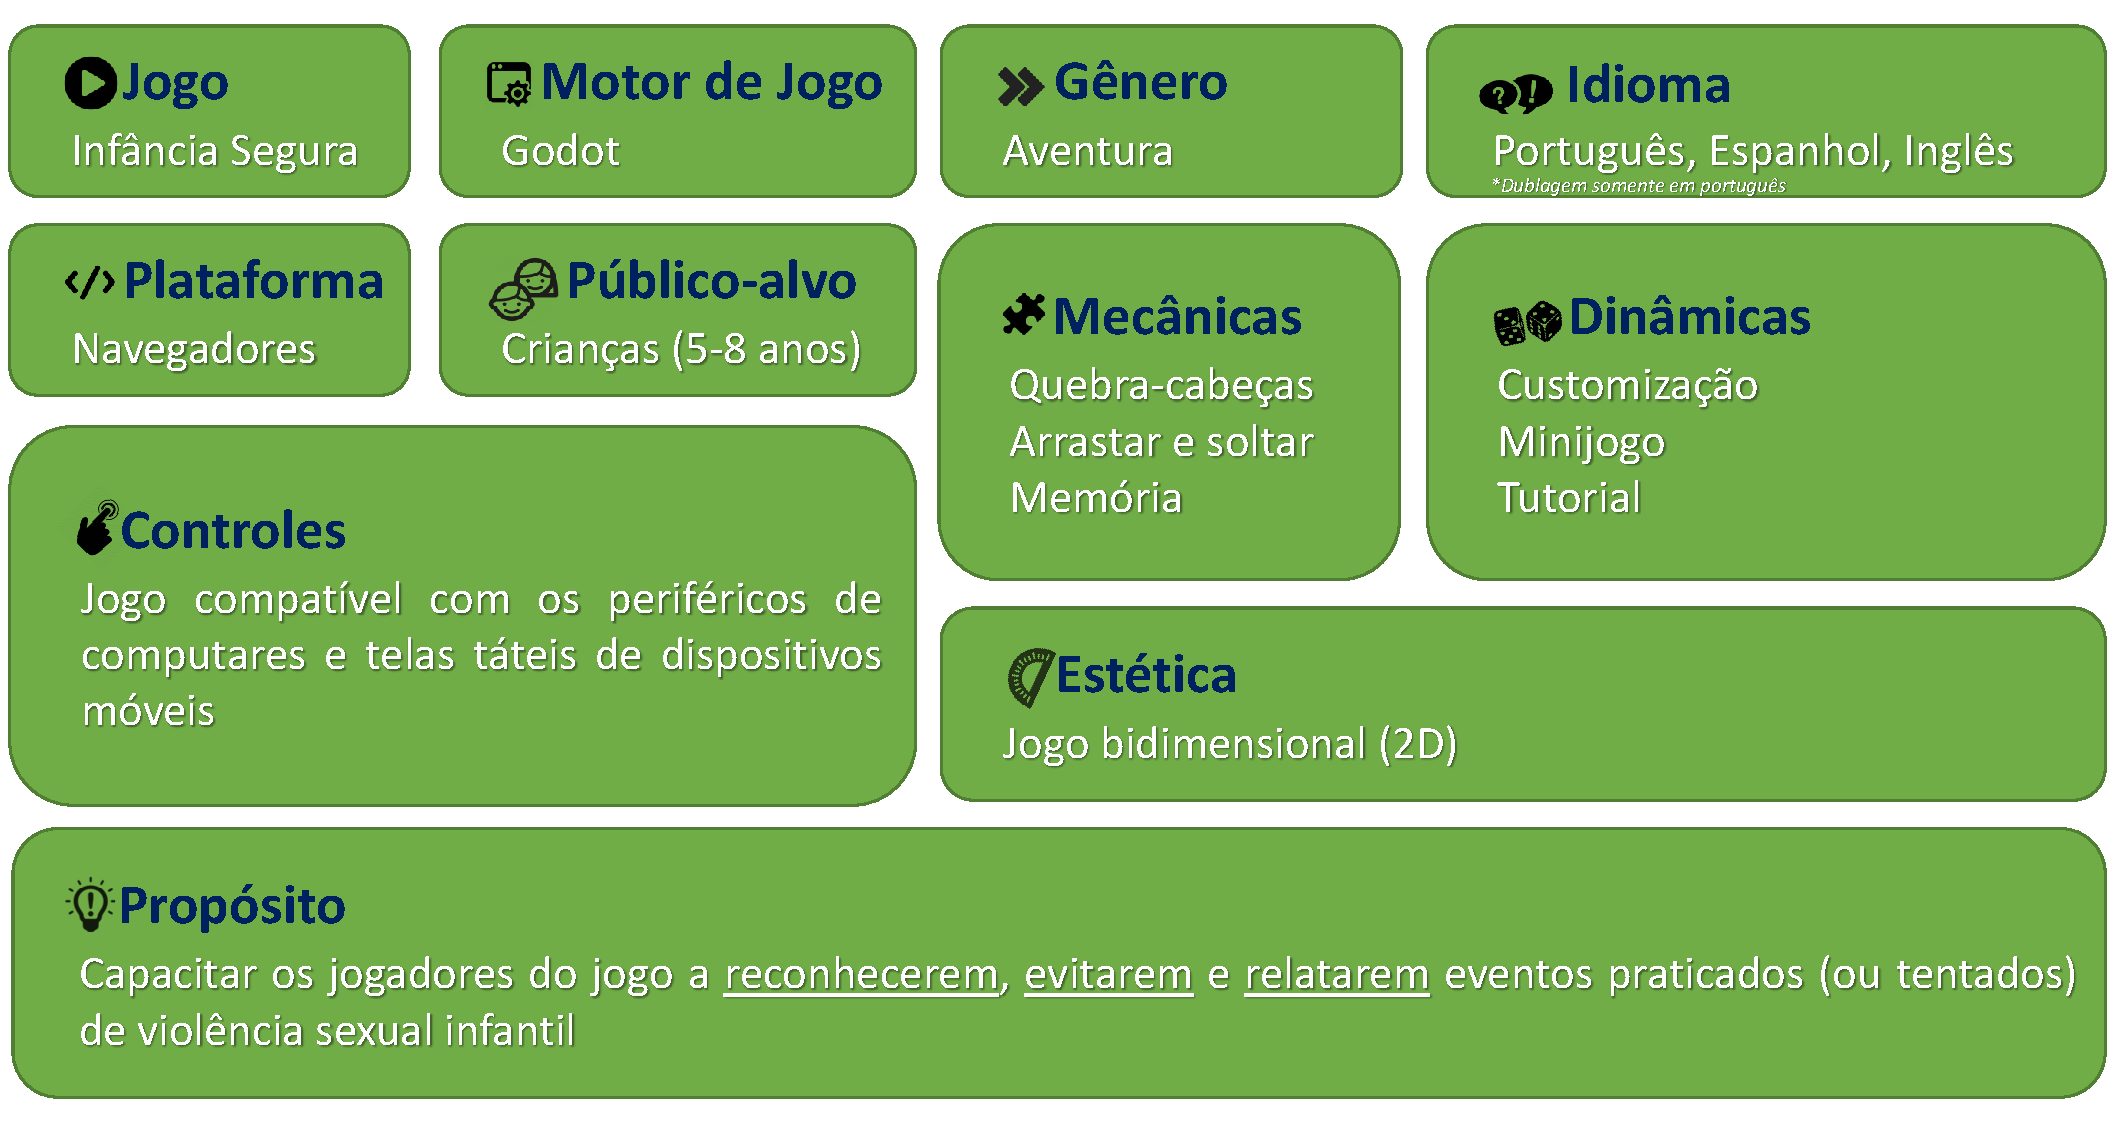
\includegraphics[width=\linewidth]{./Visuais/canvas2.pdf}
    \end{center}\vspace{-0.4cm}
  \legend{Fonte: Elaborada pelo autor (2021).}
\end{figure}

%A \autoref{fig:canvas} define as principais características do jogo desenvolvido. O jogo confecionado pelo correte trabalho herda algumas ideias propostas por \citeonline{diocesano2018infancia}, enquanto descarta outras (\textit{e.g.} o jogo original baseia-se em um dinâmica linear de exploração, ao invés de uma dinâmica de mundo aberto). Dentre os principais legados do jogo original estão: o nome do jogo, seu propósito, público-alvo e plataforma. O jogo denomina-se \textbf{Infância Segura}. Seu propósito consiste em desenvolver e aprimorar habilidades e conhecimentos específicos que viabilizem aos jogadores reconhecerem, evitarem e relatarem episódios praticados (ou tentados) de violência sexual infantil. Para atingir a classe infantil, definiu-se um público-alvo de crianças entre 5 (cinco) e 8 (oito) anos de idade. Essa idade é estabelecida com base nos conteúdos pedagógicos abordados pelo jogo, sendo conteúdos adequados a essa faixa etária de acordo com as orientações técnicas internacionais de educação em sexualidade da \citeonline{unesco2018international}. Buscando atingir um maior número de crianças, escolheu-se portar o jogo para navegadores, o que proporciona que o jogo esteja disponível a uma variedade maior de dispositivos com o mínimo de alterações ou adaptações no código-fonte \cite{carrara2018criancca}. Essa escolha, faz com que os controles do jogo sejam compatíveis aos periféricos dos computadores e as telas táteis dos dispositivos móveis.

A \autoref{fig:canvas} define as principais características do jogo desenvolvido. O jogo confecionado pelo correte trabalho herda algumas ideias propostas por \citeonline{diocesano2018infancia}, enquanto descarta outras (\textit{e.g.} o jogo original baseia-se em um dinâmica linear de exploração, ao invés de uma dinâmica de minijogos). Dentre os principais legados do jogo original estão: o nome do jogo, seu propósito, público-alvo e plataforma. O jogo denomina-se \textbf{Infância Segura}. Seu propósito consiste em desenvolver e aprimorar habilidades e conhecimentos específicos que viabilizem aos jogadores reconhecerem, evitarem e relatarem episódios praticados (ou tentados) de violência sexual infantil. Para atingir a classe infantil, definiu-se um público-alvo de crianças entre 5 (cinco) e 8 (oito) anos de idade. Essa idade é estabelecida com base nos conteúdos pedagógicos abordados pelo jogo, sendo conteúdos adequados a essa faixa etária de acordo com as orientações técnicas internacionais de educação em sexualidade da \citeonline{unesco2018international}. Buscando atingir um maior número de crianças, salienta-se que o jogo está portado para navegadores (e \textit{Android}), o que proporciona que o jogo esteja disponível a uma variedade maior de dispositivos com o mínimo de alterações ou adaptações no código-fonte \cite{carrara2018criancca}. Essa escolha, faz com que os controles do jogo sejam compatíveis aos periféricos dos computadores e as telas táteis dos dispositivos móveis.

%O jogo desenvolvido é de estética inteiramente bidimensional (2D) com perspectiva axonométrica. A bidimensionalidade do jogo agiliza o processo de desenvolvimento. A remoção uma dimensão do jogo, simplifica as etapas de programação e elaboração de cenários. Entretanto, jogos bidimensionais tendem a limitar a locomoção do personagem do jogador justamente por removerem uma dimensão. Para contornar isso, surgem os jogos em perspectiva axonométrica. Jogo axométricos, são jogos bidimensionais que não limitam a movimentação do jogador, permitindo que o mesmo possa locomover seu personagem tridimensionalmente em todo o cenário do jogo. 

O jogo desenvolvido é de estética inteiramente bidimensional (2D). A bidimensionalidade do jogo agiliza o processo de desenvolvimento. A remoção uma dimensão do jogo, simplifica as etapas de programação e elaboração de cenários. Para que o cenário e todos os demais aspectos do jogo sejam mais compreensíveis ao jogador é essencial promover um sistema de tutoria. Um sistema de tutoria auxilia o processo de compreensão das regras e da estrutura do jogo ao jogador. O esclarecimento sobre as regras e sobre a estrutura do jogo pode ser feito tanto por um tutor, quanto por um sistema de tutorial. A utilização de um sistema de tutorial substitui a necessidade de um tutor \cite{buchinger2014sherlock}. Um sistema de tutorial consite na ideia de  ensinar ao jogador como funcionam as dinâmicas de um jogo, apresentando as regras e as ações que o jogador pode exercer. Existem diversos meios para ensinar isso ao jogador. No caso do jogo desenvolvido, o sistema de tutorial utilizado segue uma estrutura simples, na qual uma certa solução inicial de uma determinada fase é apresentada ao jogador. Tal estrutura se baseia na capacidade de abstração do jogador em compreender que a solução inicial apresentada pode ser associada e replicada para as demais soluções existentes em uma determinada fase. Compreendendo os princícios básicos de uma solução, o jogador então é capaz de usar esse conhecimentos para alcançar êxito nas demais soluções de uma certa fase. 

%baseia-se na ideia de um tutor virtual que acompanha o jogador durante todo o jogo. O tutor virtual acompanha o personagem do jogador sem se distanciar muito. Isso é feito para reforçar os ensinamentos de que uma criança deve estar sempre acompanhada, além disso. %espera-se que tal funcionalidade traga um sentimento de companheirismo ao jogador. 
%Junto a este sistema de ajuda ao jogador, também é implementado a dinâmica do herói mudo. %ou dinâmica do protagonista silencioso.

%A dinâmica do herói mudo (ou protagonista silencioso) permite que o jogador tenha uma maior imersão no jogo. Nessa dinâmica, o personagem do jogador não se expressa de maneira verbal \cite{domsch2017dialogue}. Graças a isso, não há o risco do personagem do jogador se utilizar de palavras ou de elementos contextuais que o jogador desconheça, proporcionando assim, uma conexão maior entre personagem e jogador. Como artifício, para dar enredo a história do jogo, as frases são transferidas para um personagem que o jogador não possui controle (o personagem tutor), com o intuito de evitar assim, uma disrupção da interligação entre personagem e jogador. Embora o personagem do jogador não fale; todos os diálogos do jogo são transcritos textualmente e verbalmente. A depender da configuração do jogo, os diálogos podem ser exibidos em português, espanhol, ou inglês. No entanto, a verbalização dos dialógicos (localização), encontra-se disponível somente em português. A localização associada ao texto escrito proporciona acessibilidade do jogo as crianças (falantes de português) que não se encontram plenamente alfabetizadas \cite{limeira2015avaliaccao}. 

Para ajudar ainda mais o jogador, todos os diálogos do jogo são transcritos textualmente e verbalmente. A depender da configuração do jogo, os diálogos podem ser exibidos em português, espanhol, ou inglês. No entanto, a verbalização dos dialógicos (localização), encontra-se disponível somente em português. A localização associada ao texto escrito proporciona acessibilidade do jogo as crianças (falantes de português) que não se encontram plenamente alfabetizadas \cite{limeira2015avaliaccao}. 

Com o intuito de facilitar a leitura dos textos, todos os diálogos transcritos obedecem recomendações tipográficas para materiais didáticos infantis \cite{lourenco2011tipografia}. Em outras palavras, o jogo desenvolvido se utiliza e se apoia em caracteres classificados como infantis, ou seja, caracteres que se aproximam mais da escrita manual em comparação com a escrita digital (\textit{e.g.} `a' em caracter adulto, `\textit{a}' em caracter infantil).

O jogo para prevenção da violência sexual infantil projetado neste trabalho é do gênero aventura. Os jogos de aventura são jogos em que o jogador assume o papel de um protagonista em uma história interativa com exploração e resolução de quebra-cabeças. Os quebra-cabeças do presente jogo se traduzem em minijogos voltados a prevenção da violência sexual infantil. Ao se tratar do público infantil, observou-se que o gênero aventura, se destaca como o gênero de jogo que mais agrada de forma igualitária, meninos e meninas \cite{brandtzaeg2009children}. 

Os minijogos do jogo desenvolvido pela corrente pesquisa utilizam alguns elementos da cultura popular. A utilização de elementos da cultura popular no ensino é capaz aumentar os níveis de motivação e compreensão dos alunos \cite{giroux1988schooling, cheung2001use, duncan2004your, chik2011learner}. Desta forma, o jogo desenvolvido se apoia em alguns componentes da cultura popular com o intuito de melhor engajar seu público-alvo, deixando os assuntos ministrados mais interessantes e atraentes. 

Para o desenvolvimento e produção de um jogo digital, existem majoritária dois caminhos. Um jogo digital pode ser produzido em uma linguagem de programação, seguindo os protocolos e estruturas específicas de um determinado dispositivo, ou pode ser produzido sob um motor de jogo (\textit{Game Engine}). Motor de jogo é o nome dado a qualquer plataforma voltada para o desenvolvimento de jogos. Os motores de jogos proporcionam um ambiente completo para a criação de jogos, com toda a parte gráfica e sonora já abstraídas. Isso permite ao(s) desenvolvedor(es) exportar o jogo para diferentes sistemas computacionais realizando alterações mínimas no código-fonte \cite{bishop1998designing, machado2009serious}.

Existem vários motores voltados para o desenvolvimento de jogos. O motor optado por este trabalho é o \textit{Godot}\footnote{\textit{Godot} é um motor de jogos totalmente gratuito de código aberto sob a licença permissiva do MIT (CC BY 3.0). O motor pode ser adquirido por meio do seguinte endereço: \url{https://godotengine.org/}.} (versão 3.3.4). Em comparação aos demais motores de jogos, o \textit{Godot} se destaca por ser totalmente gratuito, adaptado ao idioma português e por exportar os jogos para múltiplos sistemas \cite{scherer2020analise}. Salienta-se que no momento da redação deste trabalho, a última versão estável da plataforma \textit{Godot} é a versão 3.3.4 (lançada no dia 1º outubro de 2021). Por tal razão essa é a versão que fundamenta as bases e o andamento do corrente trabalho acadêmico. Sendo utilizada a versão para \textit{Windows} 10. O ambiente de desenvolvimento do jogo assenta-se então, basicamente no sistema operacional \textit{Windows} 10 \textit{Education}. As configurações de desenvolvimento são um processador Intel(R) Core(TM) i7-8750H, 16 \acsu{GB} de memória RAM DDR4 e placa de vídeo GeForce GTX 1060. O ambiente de testes é realizado sob essas mesmas especificações, mas também em um \textit{tablet} da \textit{Multilaser} M10A, com processador Quad Core 1.3 \acsu{GHz}, 2 \acsu{GB} de memória RAM e sistema operacional \textit{Android} 8.1. Salienta-se que o \textit{tablet} utilizado para testes durante o desenvolvimento do jogo é o mesmo utilizado na etapa de testes com usuários da atual pesquisa (\autoref{ch:Avaliacao}).

Por fim, embora a plataforma \textit{Godot} exporte seus jogos para múltiplos sistemas, é importante destacar que o jogo desenvolvido neste trabalho está exportado apenas para navegadores e para o sistema \textit{Android}. Fica a cargo de pesquisa futuras a adaptação do código-fonte para portar o jogo para diferentes sistemas operacionais, possibilitando assim, que o jogo possa ser baixado e executado sem necessidade de uma conexão constante com os servidores (para outros sistemas além do \textit{Android}). Em adendo, salienta-se que a atual versão do jogo grava dados de seus jogadores em um banco de dados. O registro dos dados dos jogadores é uma herança do jogo original proposto por \citeonline{diocesano2018infancia}. Salienta-se no entanto, que os dados não são filtrados ou tratados, sendo acessíveis somente através de requisições ao servidor. Ou seja, o corrente trabalho não implemente uma ferramenta amigável para acesso dos dados dos jogadores, como proposto originalmente por \citeonline{diocesano2018infancia}. A presente pesquisa se dispõe, apenas, no desenvolvimento do jogo em si, e sua validação. Cabe então a pesquisas futuras, a confecção de uma plataforma mais agradável de acesso a essas informações, fornecendo visualização mais clara e precisa no que diz respeito ao desempenho dos jogadores, a professores ou responsáveis.  


%-------------------------------------------------------------------------------------------------------------------

\section{Desenho de Níveis e Ensinamentos}\label{sec:DN}

O \acf{JS} desenvolvido ministra assuntos sensíveis relacionados a sexualidade e a prevenção da violência sexual infantil. Por tal razão, todo o fundamental teórico do jogo advém de documentos devidamente revisados por especialistas na área de educação e sexualidade \cite{unesco2018international}. Ainda no aspecto pedagógico, salienta-se que o jogo não se utiliza de elementos visualmente realistas. Ou seja, o jogo não se utiliza de artes realistas para apresentar um determinado conceito ou uma determinada situação. A literatura relata que a utilização de imagens reais de cunho sexual trazêm desconforto para alguns indivíduos, por tal razão toda a arte utilizada no jogo assume o estilo de um cartum \cite{albert2020desenvolvimento}.

O \ac{JS} desta pesquisa possui uma estrutura metodológica de ensino baseada em quatro princípios a serem ministrados: Anatomia (\autoref{subsec:1}), Direitos (\autoref{subsec:2}), Denúncias (\autoref{subsec:3}) e Redes Sociais (\autoref{subsec:4}). Cada um desses princípios se traduz em uma fase no jogo, cada qual composta de três níveis. A \autoref{fig:conceitos} apresenta cada fase do jogo associada aos seus respectivos níveis.

\begin{figure}[hbt!]
  \caption{\label{fig:conceitos}Conceitos abordados}\vspace{-0.3cm}
  \begin{center}
    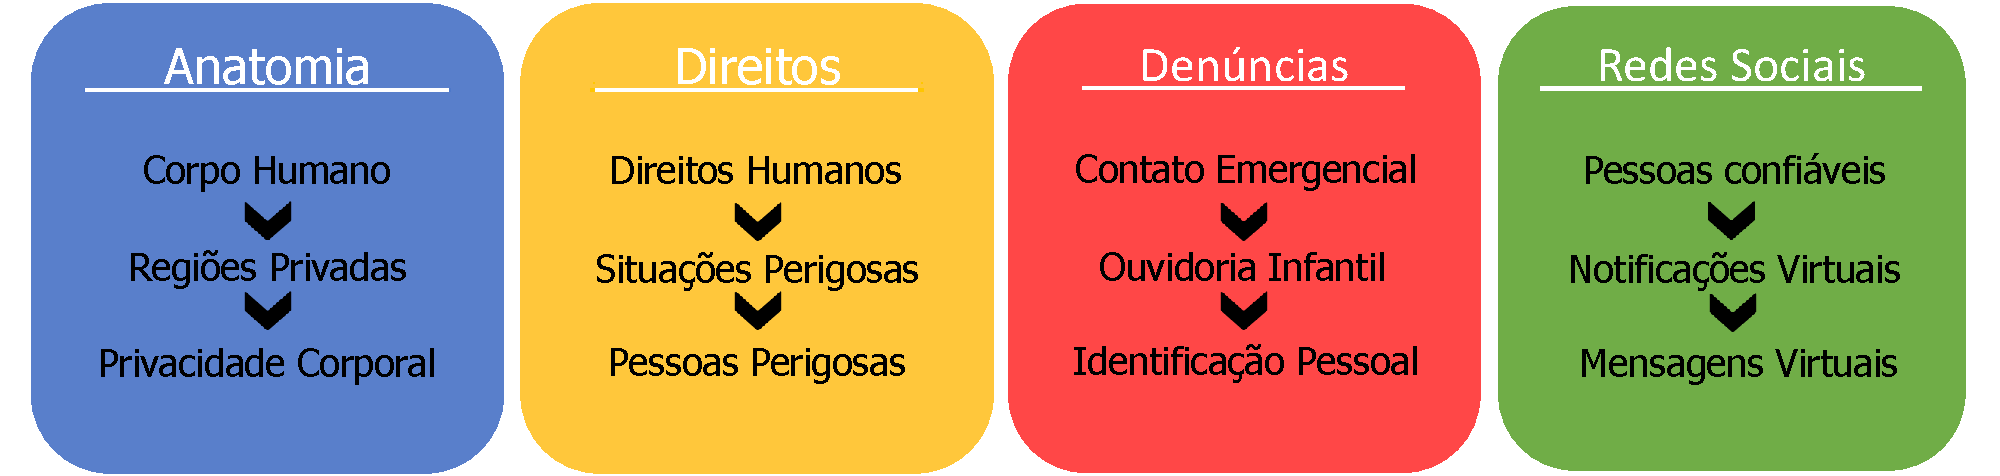
\includegraphics[width=\linewidth]{./Visuais/EsquemaFases2.pdf}
    \end{center}\vspace{-0.3cm}
  \legend{Fonte: Elaborada pelo autor (2021).}
\end{figure}

\vspace{-0.4cm}

A \autoref{fig:conceitos} ilustra de maneira resumida cada um dos conteúdos a serem ministrados pelo jogo. Cada conteúdo é ministrado em um cenários específico no jogo e por um personagem específico. O jogador é livre para intercambiar entre os cenários sem quaisquer prejuízos, podendo alternar entre as fases da maneira que melhor lhe convir. Respectivamente, os conceitos sobre anatomia são ministrados em um cenário que simula um \textbf{Hospital}. Os direitos das crianças são ensinados em um cenário que simula uma \textbf{Escola}. A realização de denúncias é um assunto ensinado em um cenário que simula uma \textbf{Delegacia}. E a proteção no ambiente virtual das redes é ministrado em cenário que simula um \textbf{Cibercafé}.

A jogabilidade de jogo é flexível, permitindo ao jogador intercambiar entre as fases sem qualquer punição. Entretanto, os níveis das fases obedecem a uma linearidade tanto de enredo, quando pedagógica (\textit{e.g.} na fase da anatomia o jogador deve necessariamente aprender antes sobre os nomes das partes do corpo, para em seguida aprender quais são as partes íntimas do corpo, para por fim aprender os locais onde as pessoas podem tocar no corpo). O jogador tem liberdade para abandonar um nível sempre que desejar. %Contudo, os últimos níveis são alcançáveis apenas após a conclusão dos anteriores. 

%-------------------------------------------------------------------------------------------------------------------

\subsection{Anatomia}\label{subsec:1}

O jogo desenvolvido ministra conteúdos relacionados a anatomia humana em um ambiente hospitalar. Três minijogos buscam ensinar ao jogador questões sobre o \textbf{Corpo Humano}, \textbf{Regiões Privadas} e \textbf{Privacidade Corporal}. A \autoref{fig:Hospitalzinho} ilustra as dinâmicas utilizadas em cada um dos minijogos. Todos os conceitos abordados por cada um destes minijogos são ministrados por um personagem que representa um médico. 

\begin{wrapfigure}[26]{r}{6.0cm}%pulando 26 linhas
  \vspace{-20pt}
  \caption{\label{fig:Hospitalzinho}Hospital}
  \includegraphics[width=\linewidth]{./Visuais/Hospital2.pdf}
  \vspace{-1.0cm}
  \legend{Fonte: Elaborada pelo autor (2021).}
\end{wrapfigure}

O primeiro minijogo (\textbf{Corpo Humano}) busca ensinar ao jogador o nome correto das partes do corpo. Com o auxílio de um mural ilustrativo, o jogador é capaz reconhecer as nomenclaturas corretas do corpo humano masculino e feminino. %Após um determinado evento, as  algumas peças do mural caem. 
O jogador deve nesse jogo demonstrar seus conhecimentos sobre o corpo humano, inserindo as peças em suas respectivas posições. As peças vão aparecendo uma a uma no centro da caixa de diálogo, sendo que o jogador deve arrastá-las e movê-las para suas posições originais. Peças colocadas em posições válidas notificam o jogador por meio se um sinal sonoro de acerto. Peças colocadas em posições inválidas emitem um aviso de erro ao jogador de forma sonora e visual. 

O segundo minijogo (\textbf{Regiões Privadas}) busca ensinar ao jogador as partes íntimas do corpo humano. O personagem do médico educa o jogador sobre as zonas privadas e não privadas do corpo, utilizando como apoio o mesmo mural do primeiro minijogo. As regiões privadas são representadas por peças com contorno vermelho no mural. Após o jogador ter adquirido esse conhecimento no tutorial, o jogo se inicia sem as peças destacadas em vermelho. Neste momento o jogador deve demonstrar suas habilidades de memorização levando os contornos vermelhos para as peças que representam as partes íntimas. A notificação de acertos e erros ao jogador ocorre da mesma maneira que no primeiro minijogo. %Peças inseridas em posições incorretas emitem sonoramente e visualmente um aviso de erro ao jogador. Peças em posições válidas emitem apenas um sinal sorono de acerto.

O terceiro minijogo (\textbf{Privacidade Corporal}) busca ensinar ao jogador sobre toques bons e ruins. Neste minijogo são apresentados dois livros, um apenas com imagens de toques bons e outro apenas com imagens de toque ruins. %Um dado evento faz com que as imagens se misturem entre os livros. 
O jogador deve demonstrar seus conhecimentos classificando devidamente as imagens. As imagens vão aparecendo uma por uma na caixa de diálogo, com o jogador tendo que movê-las para seus respectivos livros. A conclusão deste minijogo encerra a etapa de anatomia. %Após esse minijogo, o jogador completa a etapa de anatomia do jogo. 

%-------------------------------------------------------------------------------------------------------------------

\subsection{Direitos}\label{subsec:2}

O jogo projetado neste trabalho se propõe a ensinar o jogador sobre seus direitos e deveres em um cenário escolar. Três minijogos buscam ensinar ao jogador questões sobre \textbf{Direitos Humanos}, \textbf{Situações Perigosas} e \textbf{Pessoas Perigosas}. A \autoref{fig:Escola} ilustra as dinâmicas utilizadas em cada um dos minijogos. Todos os conceitos abordados são ministrados por um personagem que representa uma professora. 

\begin{wrapfigure}[26]{r}{6.0cm}%pulando 26 linhas
  \vspace{-20pt}
  \caption{\label{fig:Escola}Escola}
  \includegraphics[width=\linewidth]{./Visuais/Escola2.pdf}
  \vspace{-1.0cm}
  \legend{Fonte: Elaborada pelo autor (2021).}
\end{wrapfigure}

O primeiro minijogo (\textbf{Direitos Humanos}) busca ensinar ao jogador sobre os direitos da criança no Brasil e no mundo. O minijogo discorre sobre os direitos e deveres das crianças. Por meio de um jogo de perguntas e respostas com imagens o jogador deve associar determinado direito ou dever com uma das imagens apresentadas. O jogador então, além de ser ensinado verbalmente e textualmente sobre seus direitos, demonstra seus conhecimentos em uma representação visual. Tal método de ensino, demonstra a capacidade de abstração do jogador ao criar uma imagem mental dos conceitos aprendidos e associar essa imagem mental a uma imagem no jogo. O jogador é gratificado sonoramente por seus acertos. Quaisquer erros cometidos pelo jogador são justificados em uma mensagem sonora possibilitando que o jogador compreenda seus equívocos. 

O segundo minijogo (\textbf{Situações Perigosas}) visa educar o jogador sobre sua segurança. O jogador é ensinado que as crianças não estão totalmente protegidas de seus direitos, sendo importante tomar cuidado com determinadas situações que podem colocá-las em risco. %na qual os direitos das crianças seriam desrespeitados. 
Com o auxílio de imagens, um conjunto de situações é apresentado ao jogador onde o jogador deve optar em escolher duas situações. Nesse jogo de perguntas e respostas o jogador deve então demonstrar sua perspicácia em evitar situações potencialmente perigosas. A notificação de acertos e erros ocorre de forma igual ao primeiro minijogo.

O terceiro minijogo (\textbf{Pessoas Perigosas}) busca ensinar ao jogador sobre pessoas que podem desrespeitar os direitos das crianças. O minijogo em si realiza uma série de perguntas e respostas similar as do segundo minijogo, porém ao invés de apresentar situações, pessoas são apresentadas. Nesse minijogo, o jogador deve então demonstrar sua habilidade evitando pessoas que apresentem atitudes potencialmente perigosas. Após a conclusão deste minijogo, o jogador finaliza a etapa de direitos. 

%-------------------------------------------------------------------------------------------------------------------

\subsection{Denúncias}\label{subsec:3}

O \ac{JS} desenvolvido apresenta ao jogador algumas formas nas quais são possíveis formalizar uma denúncia. Três minijogos buscam ensinar ao jogador questões relacionadas a \textbf{Contato Emergencial}, \textbf{Ouvidoria Infantil} e \textbf{Identificação Pessoal}. A \autoref{fig:DelegaciaDP} ilustra as dinâmicas utilizadas em cada um dos minijogos. Os conceitos desse ambiente são passados por um personagem de um delegado. 

\begin{wrapfigure}[26]{r}{6.0cm}%pulando 26 linhas
  \vspace{-20pt}
  \caption{\label{fig:DelegaciaDP}Delegacia}
  \includegraphics[width=\linewidth]{./Visuais/Delegacia2.pdf}
  \vspace{-1.0cm}
  \legend{Fonte: Elaborada pelo autor (2021).}
\end{wrapfigure}


O primeiro minijogo (\textbf{Contato Emergencial}) busca apresentar ao jogador os principais telefones de emergência do Brasil. Para isso, o minijogo em questão introduz um conjunto de números telefônicos e logotipos. Nesse jogo, o jogador é instruído a associar corretamente, por intermédio de pinos, os números telefônicos e seus respectivos serviços (logotipos). Associações erradas emitem um sinal sonoro e visual ao jogador, com o pino retornando para a sua posição inicial. Associações corretas, emitem uma mensagem de acerto ao jogador, a qual explica sobre o número telefônico e sobre em quais situações tal serviço deve ser utilizado. Ao mesmo tempo, o pino se fixa ao número telefônico, não retornando a sua posição inicial.

%O primeiro minijogo (\textbf{Contato Emergencial}) busca apresentar ao jogador as formas virtuais de se realizar uma denúncia no Brasil. Para isso, o minijogo em questão introduz um computador onde um jogo de datilografia se inicia. Nesse jogo, o jogador é instruído a pesquisar e digitar corretamente os canais nacionais de denúncia. O jogo obedece uma estruturo lúdico-pedagógica de forma a ser acessível para o jogador que não encontram-se totalmente alfabetizado, acendendo as letras que devem ser selecionadas pelo jogador. Letras não acesas, selecionadas pelo jogador, não manifestam resposta (sendo um sistema de notificação de erro menos intrusivo), travando o progresso do jogador até que uma letra acesa seja selecionada. 

O segundo minijogo (\textbf{Ouvidoria Infantil}) ensina ao jogador sobre as linhas telefônicas para a denúncia de crimes contra a criança. Um mural com um número telefônico é apresentado ao jogador. %Após o jogador visualizar o mural, um dado evento, faz com que o mural se fragmente. 
Em um jogo de quebra-cabeça o jogador deve então montar o mural. A dinâmica lúdica utilizada neste jogo, prolonga o contato do jogador com o canal de denúncia do Disque 100, ampliando assim a retenção da informação. Peças colocadas em posições incorretas não provocam sinais sonoros e nem provocam sinais visuais de erro ao jogador (as peças simplesmente não se fixando no mural). Entretanto, peças colocadas em locais corretos ficam fixadas ao mural, impossibilitando de serem movidas novamente. 

%O terceiro minijogo (\textbf{Identificação Pessoal}) busca ensinar ao jogador como realizar denúncias pessoalmente e como interagir com pessoas. Neste minijogo, um livro ilustrado é apresentado ao jogador. As situações ilustradas representam eventos ordenados. Uma dada situação faz com que a ordem das ilustrações seja embaralhada. Neste momento, o jogador é confrontado a montar novamente a ordem dos acontecimentos (eventos) ilustrada no livro. 
%O jogador então demonstra como se comportar em um conjunto de situações e como relatar os acontecimentos para uma pessoa confiável. 
%O término deste minijogo, implica na conclusão da etapa de denúncias. 

O terceiro minijogo (\textbf{Identificação Pessoal}) busca ensinar ao jogador como realizar denúncias pessoalmente e como interagir com pessoas. Neste minijogo, uma pequena cidade é apresentada ao jogador, repleta de indivíduos. O jogador deve então procurar por certos indivíduos nessa cidade. Sempre que um determinado indivíduo é encontrado, uma mensagem é apresentada ao jogador, explicando sobre como interagir com determinado indivíduo, devendo manter distância ou não. O término deste minijogo, implica na conclusão da etapa de denúncias. 

%-------------------------------------------------------------------------------------------------------------------

\subsection{Redes Sociais}\label{subsec:4}

O jogo desenvolvido pela corrente pesquisa elenca, ao jogador, maneiras seguras para se proteger na \textit{internet}. Três minijogos buscam ensinar ao jogador questões sobre \textbf{Pessoas Confiáveis}, \textbf{Notificações Virtuais} e \textbf{Mensagens Virtuais}. A \autoref{fig:Cibercafe} ilustra as dinâmicas utilizadas em cada um dos minijogos. Todos os conceitos abordados por cada um destes minijogos são ministrados por um personagem de um robô. 

\begin{wrapfigure}[26]{r}{6.0cm}%pulando 26 linhas
  \vspace{-20pt}
  \caption{\label{fig:Cibercafe}Cibercafé}
  \includegraphics[width=\linewidth]{./Visuais/Cibercafe2.pdf}
  \vspace{-1.0cm}
  \legend{Fonte: Elaborada pelo autor (2021).}
\end{wrapfigure}

O primeiro minijogo (\textbf{Pessoas Confiáveis}) busca ajudar o jogador a identificar 5 (cinco) pessoas de confiança. A dinâmica deste minijogo consiste na tentativa e erro do jogador em montar um conjunto de pessoas de confiança até atingir uma combinação que esteja correta (imposta pelo minijogo). O minijogo associa as 5 (cinco) pessoas de confiança apresentadas, a outro personagem existente no jogo. Tal abordagem é tomada com o intuito de evitar associações diretas com parentes falecidos do jogador. Sendo assim, o minijogo em questão se propõe a ajudar o jogador a compreender de maneira mais genérica o que define uma pessoa confiável e o que define uma pessoa não confiável. 

%Salienta-se que minijogo evita relacionar diretamente as pessoas confiáveis (imposta pelo jogo) com pessoas reais que o jogador conheça, visando evitar associações com parentes falecidos do jogador. Sendo assim, o minijogo associa as pessoas confiáveis apresentadas a outro personagem no jogo. Durante esse minijogo as escolhas certa e erradas são justificadas ao jogador, ajudando-o a compreender o que define uma pessoa confiável e uma pessoa não confiável

O segundo minijogo (\textbf{Notificações Virtuais}) busca ensinar ao jogador como se comportar nas redes sociais. O minijogo enfatiza sobre os cuidados necessários para se acessar e se utilizar as redes sociais, salientando que algumas redes exigem uma idade mínima para sua utilização (\textit{e.g.} a rede social \textit{Facebook} define uma idade mínima de treze anos para seus usuários). A dinâmica deste minijogo consiste em ensinar ao jogador a adicionar apenas pessoas conhecidas, tendo sempre muito cuidado com a existência de perfis falsos se passando por pessoas conhecidas. O jogador precisa então, aceitar e recursar devidamente pedidos de amizade, além de aprender a desfazer amizades (caso um erro seja cometido). 

O terceiro minijogo (\textbf{Mensagens Virtuais}) ensina ao jogador como se comunicar na \textit{internet}. O minijogo se baseia no princípio que alguns serviços na \textit{internet} possibilitam o compartilhamento de mensagens sem a prévia autorização do indivíduo receptor (\textit{e.g.} o mensageiro instantâneo \textit{Whatsapp}). Desta forma, o minijogo se propõe a educar o jogador a não compartilhar informações com estranhos; relatando sempre tais acontecimentos para um adulto de confiança. Após esse minijogo, o jogador completa a etapa de Redes Sociais. 

%-------------------------------------------------------------------------------------------------------------------

\section{Considerações Finais}\label{sec:fim}

O \acf{JS} projetado por este trabalho é constituído por 12 (doze) minijogos voltados a educar crianças sobre questões relacionadas a prevenção da violência sexual infantil. Todos os minijogos, apresentam a mesma Barra de Estado (em inglês: \acl{HUD}), como pode ser observado nas telas do jogo das Figuras \ref{fig:Hospitalzinho}, \ref{fig:Escola}, \ref{fig:DelegaciaDP} e \ref{fig:Cibercafe}. A Barra de Estado, é uma região da tela do jogador na qual informações ou elementos são dispostos de modo a não atrapalhar e nem obstruir a visão do jogador, sendo anexados normalmente nas extremidades da tela na qual o jogo está sendo executado. %Os elementos da Barra de Estado do jogo desenvolvido são: um botão para silenciar/desilenciar o jogo (canto superior direito), um botão para congelar/descongelar o jogo e um botão vermelho para sair dos minijogos (centro superior). O botão vermelho situado na região superior de todos os 12 (doze) minijogos é um botão presente apenas nestes momentos. Quando o jogador está transitando entre os cenários do jogo, o botão não é apresentado. Salienta-se que um jogador só é livre para acessar e transitar livremente no jogo, após um breve cadastro. 

Os elementos da Barra de Estado do jogo desenvolvido são: um sistema de pontuação, situado no canto superior esquerdo e uma pequena engrenagem, situada no canto superior direito. O sistema de pontuação possui um opção para ser ocultado, opção essa, implementada para não estressar os jogadores ao montrar um contador continuamente na tela.
%é omitido em alguns níveis com o intuito de evitar uma maior poluição visual (\textit{e.g.} na terceira fase da Delegacia, o sistema de pontuação ocultaria a visão do jogador no que diz respeito a cidade apresentada). 
No entanto, salienta-se que, todos os níveis (com ou sem sistema de pontuação aparente) pontuam o tempo utilizado pelo jogador para a sua conclusão. Outros níveis, além de pontuarem o tempo, pontuam também a quantidade de erros cometidos pelo jogador. 

O jogo não apresenta a quantidade de erros cometidos pelo jogador no sistema de pontuação, sendo só apresentado a ``pergunta corrente'' relativa a quantidade total de perguntas. Esse artifício é utilizado por duas razões. A primeira razão, é a de evitar o constragimento do jogador, ao fixar seus erros cometidos na tela. A segunda razão, é a de deixar claro ao jogador quantas perguntas ainda devem ser respondidas, evitando assim qualquer forma de angústica relacionada ao desconhecimento sobre número de perguntas restantes para se alcançar a conclusão de um determiando nível.

O jogo desenvolvimento pelo atual trabalho exige o preenchimento de um cadastro. Neste cadastro são requisitadas duas informações: o gênero do jogador e uma credêncial de acesso. Nos níveis sobre \textbf{Anatomia} (\autoref{subsec:1}) o jogador aprende sobre as nomeclaturas e as regiões privadas do corpo humano relacionadas ao gênero que informou ao jogo. O gênero do jogador é requisitado para fornecer uma abordagem de ensino mais voltada ao indivíduo. A credêncial de acesso permite que uma determinada criança seja associada a um identificador, tal identificador se mantém em todas as etapas da corrente pesquisa. Desta forma é possível associar o desempenho de um determinado jogador no jogo e seu desempenho nas demais etapas deste trabalho. Isso tudo, sem que a devida identidade da criança tenha que ser revelada, garantindo assim seu anonimato. 

Ao final de cada nível, um relatório geral sobre o desempenho do jogador é apresentado. Nele, o jogador é capaz de identificar sua quantidade de erros e o tempo utilizada para a conclusão do nível. O jogador é convidado então a rejogar o jogo e superar seu desempenho, comentendo menos erros em um menor tempo. Salienta-se que demais informação geradas pelo sistema não são apresentados ao jogador em nenhum momento (\textit{e.g.} quaisquer ações erradas executadas pelo jogador durante o jogo). 

As informações coletadas pelo jogo servem para compreender melhor o desempenho de cada jogador e suas preferências, além de identificar eventuais dificuldades que um determinado jogador possa estar enfrentanto, proporcionando assim uma a aprendizagem mais voltada ao indivíduo, e não, ao coletivo \cite{carrara2018criancca}. Além disso, é possível identificar também, eventuais falhas conceituais ou estruturais no jogo (\textit{e.g.} caso vários jogadores manifestem o mesmo erro em um dado momento do jogo, isso pode indicar três problemas principais: ou a ação requisitada pelo jogador pode ser muito difícil e descalibrada para a sua idade; ou o sistema de pontuação do jogo pode estar classificando uma determinada ação correta como uma ação errônea; ou o pedido de ação é mal formulado sendo confuso e ambiguo para o jogador).

O jogo opera tanto para navegadores, quanto para plataformas \textit{Android}, necessitando em ambos, de  uma conexão via servidor constante durante os minijogos, para realiza requisições ao banco de dados sobre as ações dos jogadores. Visando garantir a integridade das informações; o sistema envia seus registros ao banco de dados em dois momentos. Em um momento inicial, cada ação realizada pelo jogador gera uma requisição ao banco de banco de dados, o qual armazena a ação do jogador. Em um segundo momento, ao final de um nível, o sistema envia novamente, porém em bloco, o total de ações realizada pelo jogador naquele nível, podendo assim se verificar a consitência das informações no banco de dados. Além disso, no caso das plataformas \textit{Android}, os todas essas informações são registradas e armazenadas no dispositivo no qual o jogo esteja sendo executado.

Os minijogos do jogo desenvolvido possuem seus ensinamentos baseados orientações técnicas internacionais de educação em sexualidade \cite{unesco2018international}. Os únicos dois minijogos que não encontram-se em harmonia com as orientações internacionais são os conceitos de \textbf{Contato Emergencial} e \textbf{Ouvidoria Infantil}. A introdução destes dois conceitos ao jogo, surge como uma medida de fortalecer as estratégias e campanhas nacionais de conscientização infantil. O estudo bibliográfico do presente trabalho identificou medidas nacionais focadas na divulgação dos ramais e canais de denúncia dos direitos das crianças. Almejando a divulgação de tais canais, optou-se em anexar, os dois conceitos citados, ao jogo. Com exceção destes conceitos, todos os demais assuntos estão em consonância com as orientações da \citeonline{unesco2018international}. 

Diante do exposto no presente Capítulo, enfatiza-se que o \ac{JS} desenvolvido por este trabalho baseia seus ensinamentos em conceitos didáticos reconhecidos na área em questão. Assim como, baseia seu processo de desenvolvimento em aspectos técnicos reconhecidos no campo de  desenvolvimento de jogos. O próximo passo da corrente pesquisa, consiste na realização de testes com usuários para se verificar a eficácia, ou não, do jogo no que tange o combate a violência sexual infantil. 
\chapter{Avaliação}\label{ch:Avaliacao}

No âmbito científico, a avaliação de um determinado objeto de estudo busca, de modo geral, elucidar seu real impacto e influências sobre um determinado ambiente. O presente Capítulo apresenta os principais passos tomados para a avaliação do \acf{JS} desenvolvido pelo atual trabalho. Cada etapa influente para a efetiva avaliação do jogo desenvolvido é descrita nas demais seções. Desde modo, a \autoref{sec:Preparativos} descreve sobre os principais preparativos para a execução da pesquisa, a \autoref{sec:seg} fala sobre a segmentação da amostra, a \autoref{sec:pretes} apresenta os resultados alcançados na etapa de pré-teste, a \autoref{sec:tes} os resultados do teste, a \autoref{sec:postes} os resultados do pós-teste, a \autoref{sec:apreciar} descreve os resultados obtidos na etapa de apreciação e a \autoref{sec:compilar} compila os principais resultados, comparando-os com demais trabalhos na área. 

\section{Preparativos}\label{sec:Preparativos}

A corrente pesquisa realiza a avaliação do jogo \textbf{Infância Segura}, de modo a verificar se o jogo em si é capaz de cumprir com seus preceitos pré-estabelecidos. O principal preceito do jogo consiste na ideia de que o jogo é capaz de instruir crianças entre 5 (cinco) e 8 (oito) anos a reconhecerem eventos praticados (ou tentados) de violência sexual infantil. Para tal, se faz indispensável a busca por uma amostra de crianças (dentro da faixa etária estabelecida). O conselheiro tutelar Willians Odia e a assistente social Daniella Maragno prestaram seus conhecimentos para a atual pesquisa, elencando possíveis cenários de atuação. O intercâmbio de ideias levou a Escola Municipal Pauline Parucker (Joinville/\ac{SC}). Após algumas reuniões, a escola prestou seu parecer favorável, servindo de cenário para a execução da presente pesquisa. A diretora Rafaella de Sá Moreira Botelho e a supervisora Angela Marques de Liz Souza, são as principais agentes envolvidas no processo; processo esse, firmado oficialmente pela Declaração de Ciência e Concordância das Instituições Envolvidas (\autoref{chap:DIE}). 

A Escola Municipal Pauline Parucker, se dispôs a ceder um total 112 (cento e doze) crianças para a presente pesquisa, divididas em 4 (quatro) turmas: 2º Ano C, 2º Ano D, 3º Ano C, 3º Ano D. As crianças das turmas citadas foram convidadas a participar da pesquisa. Para as crianças interessadas em participar da pesquisa foram entregues dois termos, o Termo de Assentimento (\autoref{chap:TA}) e uma versão resumida do Termo de Consentimento Livre e Esclarecido (\autoref{chap:curto}). A versão resumida do Termo de Consentimento Livre e Esclarecido surge de modo a reduzir a quantidade de documentos físicos necessários, sem reduzir de fato, seus conteúdos, isso pois, a versão resumida apresenta um endereço que eletrônico que leva ao termo na íntegra (\autoref{chap:pagina}). Após um período de duas semanas, 33 (trinta e três) documentos retornaram: 8 (oito) do 2º Ano C, 12 (doze) do 2º Ano D, 10 (dez) do 3º Ano C e 3 (três) do 3º Ano D. Salienta-se que durante esse período, um vídeo explicativo sobre a pesquisa foi enviado pela escola (via \textit{WhatsApp}) aos guardiões legais das crianças. Por fim, enfatiza-se que todos os termos e protocolos foram publicados na Plataforma Brasil, os quais foram validados e aprovados pelo Comitê de Ética, sob o \ac{CAAE} nº 43602921.2.0000.0118.

%As crianças, em suas salas de aula e em horário escolar, são apresentadas à pesquisa. Após uma breve apresentação, os menores são convidados a participar da pesquisa. Para as crianças interessadas em participar da pesquisa são entregues duas vias de dois termos. Os termos entregues são o Termo de Assentimento e o Termo de Consentimento Livre e Esclarecido. É requisitado que as crianças apresentem tais termos aos seus guardiões legais, devendo retornar uma das vias de cada um dos termos para a escola. Só participam da corrente pesquisa as crianças com toda a documentação legal devidamente atestada. Visando garantir a integridade das assinaturas e fugir de falsificações cada assinatura é comparada ao documento de matrícula escolar assinado na escola presencialmente pelos pais/responsáveis de cada criança. Todos os termos e declarações do presente estudo são impressos em duas vias. A presente pesquisa se compromete a manter guardada uma das vias por um período de 5 (cinco) anos, assim como todos os registros e resultados alcançados. O término da coleta de toda a documentação legal demarca o início do processo de segmentação da corrente pesquisa. 


\section{Segmentação}\label{sec:seg}

Ao total, 33 (trinta e três) crianças apresentaram toda a documentação necessária para participar na corrente pesquisa. Uma vez estabelecida a quantidade de indivíduos aptos a participar no corrente estudo, iniciou-se o processo de segmentação da amostra. 

A amostra foi segmentada em dois grupos: Grupo Controle e Grupo Experimental. A segmentação resultou em um grupo controle composto por 18 (dezoito) crianças e um grupo experimental composto por 15 (quinze) crianças. A disposição detalhada dos grupos ficou da seguinte maneira: grupo controle com 8 (oito) crianças do 2º Ano C e 10 (dez) crianças do 3º Ano C e grupo experimental com 12 (doze) crianças do 2º Ano D e 3 (três) crianças do 3º Ano D.


\section{Pré-teste}\label{sec:pretes}

A etapa de pré-teste do atual trabalho foi realizada no dia 19 (dezenove) de outubro de 2021 às 13h30 (hora local). A etapa de pré-teste surge na presente pesquisa com o objetivo de identificar, a existência ou não, de diferenças significativas entre o grupo controle e grupo experimental, no que diz respeito aos seus conhecimentos sobre abuso infantil. A medição dos conhecimentos das crianças é feita com auxílio do instrumento avaliativo \acf{CKAQ} adaptado ao português (\autoref{chap:traduzido}). 

A etapa de pré-teste ocorreu em dois momentos, inicialmente com as turmas do 3º (terceiro) Ano na biblioteca da escola e posteriormente com as turmas do 2º (segundo) Ano em uma sala de aula tradicional. O processo do pré-teste foi inteiramente realizado pelo presente autor com acompanhamento da supervisora Angela Marques de Liz Souza, sendo ela a responsável pela separação e remanejamento das turmas, conforme o regimento escolar. À todas as crianças foi entregue uma cópia impressa do \ac{CKAQ} adaptado ao português. Após a entrega, breves instruções sobre seu conteúdo e sua forma de preenchimento foram passadas (\autoref{chap:teste}). %(semelhante ao \autoref{chap:teste}). Qualquer dúvida poderia ser respondia com a criança levantando a mão.

O questionário foi lido em voz alta às crianças. O número da questão era lido, juntamente com seu pictograma representativo para situar as crianças sobre a pergunta corrente do questionário que deveria ser assinalada. Uma questão por vez era lida e relida, fornecendo em seguida, uma janela de tempo para as crianças deliberarem e responderem a questão. Nesse intervalo de tempo, as crianças eram indagadas se concordavam ou se discordavam do que havia sido lido, ou seja, se elas achavam verdade ou mentira a última questão lida. Para apoiar esse processo foram realizados gestos de positivo e negativo com as mãos.

O atual estudo não se dispôs a ceder material para o preenchimento do questionário (como lápis e borracha). As crianças participantes, utilizaram seus próprios materiais escolares para assinalar as questões do questionário. O processo como um todo contou com a participação de 31 (trinta e uma) crianças e durou uma hora e trinta minutos, finalizando às 15h (hora local). Cada momento de aplicação teve duração de quarenta e cinco minutos, com duas crianças faltantes do grupo controle (uma de cada turma). Ao término, as crianças retornaram a sua agenda escolar sem demais prejuízos. Por fim, os questionários foram recolhidos e levados para análise.

A análise dos dados do questionário visa compreender melhor o conhecimento de ambos os grupos no que tange os assuntos ministrados pelo questionário em si. Dentre as informações que podem ser coletados por essa análise, está a taxa de acerto por questão. Questões em branco ou rasuradas (de difícil identificação) são consideradas erradas. A corrente pesquisa computou um total de 26 (vinte e seis) questões que haviam sido deixadas em branco ou rasuradas. A taxa de acerto por questão do grupo controle pode ser observada na \autoref{fig:barrasCon}.

\begin{figure}[htb]

    \caption{\label{fig:barrasCon}Taxa de acerto por questão, pré-teste (grupo controle).}
    \includegraphics[width=\linewidth]{./Visuais/Notas4.pdf}
    \legend{Fonte: Elaborada pelo autor (2021).}
  
\end{figure}

A \autoref{fig:barrasCon} ilustra a taxa de acerto por questão (grupo controle). O eixo das abscissas representa cada uma das questões do questionário, sendo o número 1 (um) a primeira questão do questionário e o número 33 (trinta e três) a última questão do questionário. O eixo das ordenadas representa a taxa de acerto, indo de 0 (zero) a 100 (cem). O número 0 (zero) significa que nenhum indivíduo acertou aquela questão, o número 100 (cem) significa que todos os indivíduos acertaram aquela questão. No presente caso, tanto a questão 4 (quatro), quanto a questão 31 (trinta e um), tiveram uma taxa de acerto de 100\% para o grupo controle. O mesmo não ocorre com o grupo experimental como pode ser observado na \autoref{fig:barrasExp}.

\begin{figure}[htb]

    \caption{\label{fig:barrasExp}Taxa de acerto por questão, pré-teste (grupo experimental).}
    \includegraphics[width=\linewidth]{./Visuais/Notas3.pdf}
    \legend{Fonte: Elaborada pelo autor (2021).}
  
\end{figure}

A \autoref{fig:barrasExp} apresenta a taxa de acerto por questão (grupo experimental). Em comparação ao grupo controle (\autoref{fig:barrasCon}) o grupo experimental teve um desempenho ligeiramente inferior. Buscando fornecer um panorama melhor dos resultados alcançados nessa etapa, produziu-se um diagrama de caixa estreita (\autoref{fig:caixaprePRE}).

\begin{wrapfigure}[15]{r}{9.0cm}%pulando 15 linhas
    \vspace{-4pt}
    \caption{\label{fig:caixaprePRE}Diagrama geral das notas, pré-teste.}
    \includegraphics[width=\linewidth]{./Visuais/CaixaEstreitaEnfeitado.pdf}
    \legend{Fonte: Elaborada pelo autor (2021).}
\end{wrapfigure}

Um diagrama de caixa mostra a distribuição dos dados em quartis, realçando a média e as exceções. No caso do presente estudo o grupo controle acertou em média 19,625 ($\sigma$ = 3,18) questões (59,47\%, $\sigma$ = 9,64), enquanto o grupo experimental acertou em média 17,467 ($\sigma$ = 3,96) questões (52,93\%, $\sigma$ = 12), valores representados pela marcação em $\times$ na \autoref{fig:caixaprePRE}. A maior quantidade de acertos foi de 26 (vinte e seis) questões no grupo controle e 24 (vinte e quatro) questões no grupo experimental. Ambos os grupos tiveram uma menor quantidade de acertos de 13 (treze) questões.

A análise feita das amostras serve de apoio para uma compreensão básica dos grupos estudados, todavia os cálculos realizados não são suficientes para alcançar conclusões mais robustas. Além de calcular tais valores, é preciso interpretá-los estatisticamente. Por tanto, para a devida condução da atual pesquisa é necessário interpretar se há equivalência ou diferença estatística entre as amostras. Nesse sentido, a estatística possui um conjunto de testes para averiguar o grau de equivalência entre duas amostras. %Alguns testes estatíticos necessitam que determinados critérios sejam cumpridos para que o teste em si seja realizado sem erros. 

O presente estudo se utiliza de dois testes estatísticos, um para calcular a média ($\overline{\times}$) e outro para calcular a mediana ($\tilde{\times}$). Para o cálculo da mediana o corrente trabalho acadêmico se utilizou do teste de \textit{Mann-Whitney}. O teste compara duas amostras independentes, de modo a calcular se há equivalência entre suas medianas. Dito isso, o atual estudo fez uso do teste de \textit{Mann-Whitney} para determinar, a existência ou não, de equivalência entre as medianas do grupo controle e do grupo experimental. Os cálculos apontaram para uma equivalência entre as amostras (U = 64; p = 0,08323). Desta forma a hipótese nula (H$_0$) do teste de \textit{Mann-Whitney} deve ser aceita, indicando que as medianas entre os grupos são equivalentes (\textit{M}$_{controle}$ = \textit{M}$_{experimental}$). %com 95\% de confiança de

Para o cálculo da média o presente estudo se utilizou do Teste \textit{t}. O Teste \textit{t} é considerado exato e adequado para a hipótese de igualdade de médias. No entanto, o Teste \textit{t} exige que alguns critérios sejam cumpridos para que seus resultados tenham validade estatística. Um destes critérios exige que os dados das amostras devem obedecer uma distribuição normal. Nesse sentido, a presente pesquisa se utilizou de dois testes de normalidade, o teste de \textit{Shapiro-Wilk} e o teste de \textit{D'Agostino-Pearson}, ambos indicaram que  os dados colhidos obedecem uma distribuição normal. Outro critério exigido pelo Teste \textit{t} diz respeito a variância das amostras. Os cálculos realizados indicaram que as variâncias do grupo controle e grupo experimental são equivalentes ($\alpha$ = 5\%). Deste modo, o Teste \textit{t} pode ser realizado, concluindo ao final que as amostras são de fato, equivalentes ($\alpha$ = 5\%). A \autoref{fig:normal} ilustra a equivalência entre as amostras. 

\begin{figure}[htb]
    \centering
    \caption{\label{fig:normal}Distribuição das notas atingidas, pré-teste.}
    \includegraphics[width=\linewidth]{./Visuais/Graficos1.pdf}
    \legend{Fonte: Elaborada pelo autor (2021).}
  
\end{figure}

A \autoref{fig:normal} ilustra as distribuições normais do grupo controle e do grupo experimental. O eixo das abscissas representa o total de acertos no questionário, indo de 0 (zero) até 33 (trinta e três), tal escala indica a quantidade de questões assinaladas corretamente no questionário. Já o eixo das ordenadas representa a probabilidade da quantidade de acertos. Os máximos globais de cada grupo, são as médias já calculadas e ilustradas na \autoref{fig:caixaprePRE}.

O Teste \textit{t} mostrou que não há diferenças significativas entre as médias das amostras (t$_{(27)}$ = 1,655; p = 0,10953). Ou seja, os resultados do Teste \textit{t} indicam não haver diferenças de conhecimento entre as crianças do grupo controle e as crianças do grupo experimental, no que diz respeito aos conhecimentos medidos pelo instrumento avaliativo \ac{CKAQ}. Desta forma a hipótese nula (H$_0$) do Teste \textit{t} deve ser aceita, indicando que não existe diferenças entre as médias das amostras ($\mu$$_{controle}$ = $\mu$$_{experimental}$). 

Os resultados alcançados nessa seção apontam; tanto para uma média, quanto para uma mediana, equivalente entre as amostras. Notoriamente, os cálculos matemáticos realizados pela presente pesquisa não estão isentos de falhas, portanto, com intuito de facilitar a revisão dos resultados alcançados, e com intuito de deixar todo o processo mais transparente o possível a corrente pesquisa publica todos os dados obtidos nessa etapa no \autoref{chap:resul1}.

Por fim, é importante salientar que os resultados alcançados na etapa de pré-teste da atual pesquisa correspondem aos resultados esperados para essa etapa. Isso pois, o corrente trabalho, só poderia prosseguir com a pesquisa caso as amostras estudadas fossem equivalentes. Sendo as amostras equivalentes, o jogo desenvolvido pelo atual trabalho pode então, ser aplicado ao grupo experimental na etapa de teste da corrente pesquisa (\autoref{sec:tes}).


\section{Teste}\label{sec:tes}

A etapa de teste do atual trabalho ocorreu em três momentos distintos; dia 3 (três), dia 4 (quatro) e dia 5 (cinco) de novembro de 2021. No dia 3 (três) foram realizados os preparativos para a instalação do jogo nos \textit{tablets} da escola (modelo \textit{Multilaser} M10A). O processo se iniciou às 14h e terminou às 16h15 (hora local). O processo de instalação do jogo nos \textit{tablets} se deu na biblioteca da escola e contou com a participação da professora Carla Diacui Medeiros Berkenbrock, a supervisora Angela Marques de Liz Souza e o presente autor desta dissertação. Ao total o jogo foi instalado em 30 (trinta) \textit{tablets}. Foi realizada a instalação do jogo em mais \textit{tablets} do que o necessário, visando contornar demais empecilhos como problemas ou falta de energia em algum determinado dispositivo durante a etapa de teste (apenas um \textit{tablet} foi trocado durante os experimentos). %Ao final, todos os \textit{tablets} foram colocados em um gabinete de recarga.

Nos dias 4 (quatro) e 5 (cinco) de novembro de 2021 a presente pesquisa conduziu sua etapa de teste com crianças (na bilioteca da escola). O processo consistiu em submeter aos participantes (crianças), o objeto estudado (jogo). No dia 4 (quatro) as crianças participantes foram instruidas a jogar o jogo \textbf{Infância Segura}, mais especificamente as fases sobre \textbf{Direitos} (\autoref{subsec:2}) e \textbf{Denúncias} (\autoref{subsec:3}). No dia 5 (cinco) as crianças foram instruidas a jogar as demais fases, sobre \textbf{Anatomia} (\autoref{subsec:1}) e \textbf{Redes Sociais} (\autoref{subsec:4}). Essa separação das fases foi uma sugestão da supervisora Angela. É importante salientar que a etapa de teste foi conduzida inteiramente e apenas com as crianças do grupo experimental, com uma criança do 3º Ano D faltante no dia 5 (cinco). Em ambos os dias o processo se iniciou às 13h40.

No dia 4 (quatro) e no dia 5 (cinco) os \textit{tablets} foram distribuídos sobre as mesas da biblioteca da escola. As crianças foram entrando, duas a duas, na biblioteca da escola, sendo instruídas a sentarem na frente do \textit{tablet} que contivesse uma etiqueta com seu nome escrito (no último dia a posição dos \textit{tablets} foi trocada). Em ambos os dias as crianças tiveram contato com o jogo por quarenta e cinco minutos, totalizando ao total uma hora e trinta minutos de atividades (com início às 14h15 e término às 15h). O processo foi inteiramente conduzido pelo presente autor desta dissertação, com auxílio da supervisora Angela (todos os dias). Em separado, no 4 (quatro) a pesquisadora responsável Carla Diacui Medeiros Berkenbrock e no dia 5 (cinco) a aposentada Rocilda Cordeiro Mendonça, prestaram sua atenção e auxílio a pesquisa. Em específico a supervisora Angela foi a responsável pelo remanejamento dos estudantes. %Em específico a suprevisora Angela foi a responsável por remanejar os estudantes das suas salas à biblioteca (e vice-versa).

No primeiro dia, as crianças foram apresentadas ao jogo com auxílio de um projetor. Neste momento as crianças foram instruídas a se identificarem no jogo e a informarem seu gênero. As crianças também foram instruídas a como alterar o volume do jogo e a como intercambiar entre as fases. No segundo dia, com auxílio do mesmo projetor, realizou-se uma revisão do terceiro minijogo da fase sobre \textbf{Direitos} e do primeiro minijogo da fase sobre \textbf{Redes Sociais}. Tais minijogos foram escolhidos para uma revisão, uma vez observado que os conteúdos contidos nestes minijogos coincidiam com os conteúdos das questões com menores taxas de acerto para o grupo experimental na etapa de pré-teste (\autoref{sec:pretes}).

No segundo dia, as crianças (em geral) apresentaram muita dificuldade para concluir o primeiro e o segundo minijogo da fase sobre \textbf{Anatomia}. Em virtude dessa dificuldade, instruções mais detalhadas de cada minijogo foram passadas com auxílio de um projetor. Por fim, a taxa de conclusão do jogo (quatro fases) ficou em 89,63\%. Ao todo 7 (sete) crianças deixaram de concluir uma ou mais fases no jogo. Os minijogos da etapa de \textbf{Direitos} e \textbf{Redes Sociais} foram os minijogos com melhor desempenho entre os jogadores. Seguidos pelos minijogos da etapa de \textbf{Denúncias} e pelos minijogos da etapa de \textbf{Anatomia}, com os piores desempenhos. 

No segundo dia, a rede sem fio da escola apresentou instabilidade. Tal instabilidade impossibilitou que os dados dos estudantes (gerados durante o jogo) fossem enviados aos servidores da aplicação. No entanto, os dados gerados pelos jogadores durante a etapa de teste, além de estarem programados para serem enviados a um banco de dados, também estavam programados para armazenar todo conjunto de ações dos seus jogadores localmente (nos \textit{tablets}). Com isso, após o fim dos experimentos no segundo dia, o conteúdo de cada jogador foi extraído dos \textit{tablets} (o processo levou em torno de uma hora). Por fim, a etiqueta dos tablet foi removida, os \textit{tablets} foram desligados e colocados em um gabinete de recarga. Ao total, 3.315 ações foram computadas nos minijogos, dando em média, 221,83 ações por jogador.

Durante a etapa de teste, nenhum dos envolvidos manifestou qualquer quadro de angústia, nervosismo, ansiedade ou constrangimento para com os conteúdos abordados pelo jogo. Destaca-se apenas que, uma das crianças, apresentou sinais de preocupação, ao sentir que estava demorando mais do que os seus outros colegas para concluir os minijogos. Também destaca-se que, algumas crianças, tiveram dificuldades em compreender os diálogos do jogo, pedindo muitas vezes, para que os diálogos fossem lidos para elas. O fato de muitas crianças não estarem plenamente alfabetizadas, acabou por atrapalhar a absorção do conteúdo pelas crianças. Isso pois, por mais que o jogo estivesse localizado em português, a execução conjunta  dos \textit{tablets} em um mesmo ambiente acabou gerando um certo ruído sonoro no ambiente, dificultando os áudios de serem ouvidos. As crianças levantavam suas mãos quando necessitavam de alguma ajuda ou auxílio, quando precisavam ir ao banheiro ou quando gostariam de informar que concluíram com todo o conteúdo. As crianças que manifestaram terem concluído todo o jogo foram liberadas a jogar qualquer minijogo de seu interesse (até o término das atividades). 

O jogo em si apresentou algumas falhas de desenvolvimento durante a etapa de teste. Nesse sentido, falhas tanto técnicas, quanto conceituais foram constatadas. Tais observações geraram ideias de aperfeiçoamento e melhorias, as quais foram manifestadas pelos profissionais envolvidos na corrente pesquisa. Tais ideias são descritas no \autoref{ch:Conclusao} do presente trabalho acadêmico, de modo a compilar conjuntamente as ideias manifestadas pelas crianças do grupo experimental. 

 
\section{Pós-teste}\label{sec:postes}

A etapa de pós-teste do corrente trabalho foi conduzida no dia 22 (vinte e dois) de novembro de 2021 às 13h50 (hora local). A etapa de pós-teste surge na presente pesquisa com o objetivo de identificar, a existência ou não, de diferenças significativas entre o grupo controle e grupo experimental, no que diz respeito aos seus conhecimentos sobre abuso infantil. A medição dos conhecimentos das crianças é feita com auxílio do instrumento avaliativo \acf{CKAQ} adaptado ao português (\autoref{chap:traduzido}). 

A etapa de pós-teste ocorreu em dois momentos, inicialmente com o grupo experimental na biblioteca da escola e posteriomente com o grupo controle em uma sala de aula tradicional. O processo do pós-teste foi inteiramente realizado pelo presente autor com acompanhamento da pesquisadora responsável Carla Diacui Medeiros Berkenbrock e da supervisora Angela Marques de Liz Souza, sendo ela a responsável pela separação e remanejamento das turmas, conforme o regimento escolar. À todas as crianças foi entregue uma cópia impressa do \ac{CKAQ} adaptado ao português. Após a entrega, breves instruções sobre seu conteúdo e sua forma de preenchimento foram passadas (\autoref{chap:teste}).

O questionário foi lido em voz alta as crianças. O número da questão era lido, juntamente com seu pictograma representativo para situar as crianças sobre a pergunta corrente do questionário que deveria ser assinalada. Uma questão por vez era lida e relida, fornecendo em seguida, uma janela de tempo para as crianças deliberarem e responderem a questão. Nesse intervalo de tempo, as crianças eram indagadas se concordavam ou se discordavam do que havia sido lido, ou seja, se elas achavam verdade ou mentira a última questão lida. Para apoiar esse processo foram realizados gestos de positivo e negativo com as mãos.

O presente estudo não se dispôs a ceder material para o preenchimento do questionário (como lápis e borracha). As crianças participantes, utilizaram seus próprios materiais escolares para assinalar as questões do questionário. O processo como um todo contou com a participação de 29 (vinte e nove) crianças e durou uma hora (com término às 14h20 para o grupo experimental e às 16h30 com o grupo controle). Cada momento de aplicação do questionário teve duração de trinta minutos, com quatro crianças faltantes (uma de cada turma). Ao término, as crianças do grupo controle retornaram a sua agenda escolar sem demais prejuízos, já as crianças do grupo experimental passaram por uma etapa a mais da corrente pesquisa, a qual é descrita mais detalhadamente no \autoref{sec:apreciar}. Todavia, antes de dar andamento para a próxima etapa da pesquisa, é preciso analisar e interpretar os dados gerados na presente etapa. 

Após a coleta e análise dos questionários a corrente pesquisa computou um total de 7 (sete) questões deixadas em branco ou rasuradas. Tal como na etapa de pré-teste (\autoref{sec:pretes}) a etapa de pós-teste também compila as taxas de acerto por questão do grupo controle e do grupo experimental, permitindo assim, uma comparação mais detalhada e acurada entre os desenvolvimentos internos de cada grupo. A taxa de acerto por questão do grupo controle pode ser observada na  \autoref{fig:barrasCon1}.


\begin{figure}[htb]

    \caption{\label{fig:barrasCon1}Taxa de acerto por questão, pós-teste (grupo controle).}
    \includegraphics[width=\linewidth]{./Visuais/NotasControlePOS.pdf}
    \legend{Fonte: Elaborada pelo autor (2021).}
  
\end{figure}

A \autoref{fig:barrasCon1} revela que as crianças do grupo controle mantiveram uma taxa de acerto de 100\% para a questão 4 (quatro), todavia em relação ao pré-teste, as crianças não mantiveram o mesmo desempenho para a questão 31 (trinta e um). Em síntese observou-se uma ligeira evolução de desempenho entre o pré e o pós-teste. Ao total 16 (dezesseis) questões foram computadas com um desempenho superior ao constatado na etapa de pré-teste para o grupo controle. 
%As questões que tiveram um desempenho superior são as questões: 3, 5, 10, 11, 13, 14, 15, 16, 19, 21, 23, 24, 26, 29, 30, 33
No entanto, um desempenho mais acentuado é observado no grupo experimental como ilustra o gráfico em barras da \autoref{fig:barrasExp1}.


\begin{figure}[htb]

    \caption{\label{fig:barrasExp1}Taxa de acerto por questão, pós-teste (grupo experimental).}
    \includegraphics[width=\linewidth]{./Visuais/NotasExperimentalPOS.pdf}
    \legend{Fonte: Elaborada pelo autor (2021).}
  
\end{figure}

A \autoref{fig:barrasExp1} revela que as crianças do grupo experimental tiveram uma taxa de acerto de 100\% para a questão 4 (quatro), 10 (dez) e 19 (dezenove).  Em síntese observou-se uma evolução de desempenho entre o pré e o pós-teste do grupo experimental. Ao total 20 (vinte) questões foram computadas com um desempenho superior ao constatado na etapa de pré-teste.
%As questões que tiveram um desempenho superior são as questões: 3, 4, 5, 6, 10, 11, 12, 14, 15, 17, 18, 19, 22, 23, 25, 26, 27, 28, 31, 32.
As crianças do grupo experimental manifestam um progresso mais expressivo de desempenho quando comparadas com o grupo controle. Todavia, a evolução interna dos grupos não se destaca, quando as amostras são comparadas entre si. Nesse sentido, para fornecer um panorama melhor dos resultados alcançados nessa etapa da pesquisa, produziu-se um diagrama de caixa estreita, ilustrado na \autoref{fig:caixapre1}.

\begin{wrapfigure}[15]{r}{9.0cm}%pulando 15 linhas
    \vspace{-4pt}
    \caption{\label{fig:caixapre1}Diagrama geral das notas, pós-teste.}
    \includegraphics[width=\linewidth]{./Visuais/CaixaEstreitaPOS.pdf}
    \legend{Fonte: Elaborada pelo autor (2021).}
\end{wrapfigure}

Os resultados do diagrama de caixa estreita mostram que o grupo controle teve uma taxa de acerto média 21,312 ($\sigma$ = 4,28) questões (64,58\%, $\sigma$ = 12,98), enquanto o grupo experimental teve uma taxa de acerto média 19,308 ($\sigma$ = 5,45) questões (58,51\%, $\sigma$ = 16,52), valores representados pela marcação em $\times$ na \autoref{fig:caixapre1}. A maior quantidade de acertos foi de 30 (trinta) questões no grupo controle e 27 (vinte e sete) questões no grupo experimental. Com uma quantidade mínima de acertos de 12 (doze) para o grupo experimental e 14 (catorze) para o grupo controle.

Considerando as médias de acertos no questionário entre os grupos, a \autoref{fig:caixapre1} mostra que o grupo controle não supera o grupo experimental. Todavia, considerando as medianas entre os grupos, é possível observar que o grupo experimental supera a mediana do grupo controle. Por tal razão, a presente pesquisa se prestou a ampliar sua abordagem metodológica (\autoref{sub:Finalidade}), se utilizando além de testes estatísticos para o cálculo das médias entre os grupos, testes estatísticos para o cálculo de suas medianas. 

Para o cálculo da mediana, o presente estudo se utilizou do teste de \textit{Mann-Whitney}, assim como na etapa de pré-teste (\autoref{sec:pretes}). Os cálculos alcançados apontaram para uma equivalência entre as amostras (U = 86; p = 0,44488). Desta forma a hipótese nula (H$_0$) do teste de \textit{Mann-Whitney} deve ser aceita, indicando com 95\% de confiança de que as medianas entre os grupos são equivalentes (\textit{M}$_{controle}$ = \textit{M}$_{experimental}$). 

Para o cálculo da média, a corrente pesquisa fez uso do Teste \textit{t}. Como informado na etapa de pré-teste (\autoref{sec:pretes}), o Teste \textit{t} exige que certos critérios devam ser atendidos para que os resultados alcançados pelo teste tenham validade estatística. Um destes critérios é a condição de normalidade das amostras. Nesse sentido, tanto o teste de \textit{Shapiro-Wilk}, quanto o teste de \textit{D'Agostino-Pearson} indicaram que os informações colhidas e computadas das amostras obedecem uma distribuição normal. 

A variância das amostras também foi computada para a devida execução do Teste \textit{t}. O resultado das variâncias apontou ao final que as variâncias do grupo controle e do grupo experimental são equivalentes ($\alpha$ = 5\%). Deste modo, o Teste \textit{t} pode ser realizado, concluindo ao término que as amostras são de fato, equivalentes ($\alpha$ = 5\%). A \autoref{fig:normal} ilustra a equivalência entre as amostras.

\pagebreak

\begin{figure}[htb]
    \centering
    \caption{\label{fig:normal1}Distribuição das notas atingidas, pós-teste.}
    \includegraphics[width=\linewidth]{./Visuais/GraficosPosteste.pdf}
    \legend{Fonte: Elaborada pelo autor (2021).}
\end{figure}


O Teste \textit{t} mostrou que não há diferenças significativas entre as médias das amostras (t$_{(27)}$ = 1,109; p = 0,27697). Ou seja, os resultados do Teste \textit{t} indicam não haver diferenças de conhecimento entre as crianças do grupo controle e as crianças do grupo experimental, no que diz respeito aos conhecimentos medidos pelo instrumento avaliativo \ac{CKAQ}. Desta forma a hipótese nula (H$_0$) do Teste \textit{t} deve ser aceita, indicando que não existem diferenças entre as médias das amostras ($\mu$$_{controle}$ = $\mu$$_{experimental}$). %Os máximos globais de cada grupo, são as médias já calculadas e ilustradas na \autoref{fig:caixapre1}. 
Um comparativo da evolução de desempenho dos grupos entre o pré e o pós-teste pode ser observado na \autoref{fig:normal2}.

\begin{figure}[htb]
    \centering
    \caption{\label{fig:normal2}Distribuição comparativa, pré-teste e pós-teste.}
    \includegraphics[width=\linewidth]{./Visuais/GraficosAntesDepois.pdf}
    \legend{Fonte: Elaborada pelo autor (2021).}
\end{figure}

A \autoref{fig:normal2} apresenta as curvas normais de ambos os grupos estudados. De forma mais nítidas são representadas as curvas da etapa de pós-teste, as demais curvas representam a etapa de pré-teste. Comparando o pré com o pós-teste é possível constatar que ambas as curvas ficaram mais achatadas, indicando uma maior dispersão da quantidade de questões acertadas. 

Os resultados alcançados nessa seção apontam; tanto para uma média, quanto para uma mediana, equivalente entre as amostras. Sendo assim, a \hyperref[hipotese]{hipótese nula} (H$_0$) da corrente pesquisa deve ser aceita, rejeitando-se a hipótese alternativa (H$_1$). Desta forma é possível inferir com um grau de confiança de 95\% que o programa educacional desenvolvido nessa pesquisa não foi capaz de influenciar estatisticamente o grupo experimental (nem positivamente, nem negativamente). Ou seja, o jogo desenvolvido pela presente pesquisa não aparenta ter interferido estatisticamente no conhecimento das crianças do grupo experimental em relação aos conhecimentos do grupo controle no que diz respeito aos conhecimentos medidos pelo instrumento avaliativo \ac{CKAQ}. As implicações sobre esse resultado são deliberadas mais detalhadamente na \autoref{ch:Conclusao} do presente trabalho acadêmico.

Uma vez constatada a equivalência das médias e das medianas entre os grupos, a atual pesquisa se dispôs a calcular também, suas relações internas, comparando os resultados pareados na etapa de pré-teste em comparação a etapa de pós-teste. Além disso, a corrente pesquisa também buscou identificar possíveis relações entre o desempenho das crianças no jogo e suas pontuações atingidas no questionário \ac{CKAQ}. Nesse sentido, observou-se que o jogador com o melhor desempenho no jogo, obteve uma pontuação média no questionário de 17 (dezessete) acertos. Por tal razão, não é possível estabelecer qualquer relação entre o jogo desenvolvido por essa pesquisa e o questionário aplicado. 

%O presente estudo também se dispós a medir a relação interna do grupo experimental, verificando não apenas seu desempenho na etapa de pré-teste em relação etapa de pós-teste, mas também encontrar possíveis relações de desemenho no jogar dos jogo pelas crianças (o presente estudo também relaciona as variáveis de desempenho e aprendizagem a fim de encontrar relações entre o desempenho de determinados indivíduos em um jogo e o aprimoramento de suas habilidades intelectuais no que diz respeito aos assuntos ministrados pelo jogo.) Nesse sentido, observou-se que a criança com a menor taxa de erros durante os teste com o jogo, foi a criança com menor desempenho no questionário (12 acertos). E a criança com a maior taxa de acertos durante os testes com o jogo, teve um desempenho médio no questionário (17 acertos). Por tal razão, nada se pode afirmar sobre uma possivel associação entre o desempenho das crianças no jogo e seu desempenho no questionario. Nenhuma relação foi identificada, portanto nenhum gráfico ou estatísticas foram gerados. 

As relações internas do grupo experimental foram calculadas com auxílio do Teste \textit{t} e do teste de \textit{Wilcoxon}. O teste de \textit{Wilcoxon} é um teste para amostras relacionadas, usado para comparar suas medianas. Os cálculos com o teste de \textit{Wilcoxon} apontaram que as medianas entre o pré e o pós-teste do grupo experimental são de fato equivalentes (z = 1,06312; p = 0,30127). Desta forma a hipótese nula (H$_0$) do teste de \textit{Wilcoxon} deve ser aceita, indicando com 95\% de confiança de que as medianas são equivalantes (\textit{M}$_{pr\acute{e}-experimental}$ = \textit{M}$_{p\acute{o}s-experimental}$). 

O Teste \textit{t} para amostras relacionadas mostrou que não há diferenças significativas de conhecimento entre o pré e pós-teste do grupo experimental, no que tange os conhecimentos medidos pelo instrumento avaliativo \ac{CKAQ} (t$_{(12)}$ = -1,38873; p = 0,19015). Desta forma a hipótese nula (H$_0$) do Teste \textit{t} deve ser aceita, indicando que não existe diferenças significativas ($\alpha$ = 5\%) entre as médias ($\mu$$_{pr\acute{e}-experimental}$ = $\mu$$_{p\acute{o}s-experimental}$).

Os resultados alcançados nessa seção apontam; tanto para uma média, quanto para uma mediana, equivalente entre as amostras (e entre as etapas de pré e pós-teste para o grupo experimental). Notoriamente, os cálculos matemáticos realizados pela presente pesquisa não estão isentos de falhas, portanto, com intuito de facilitar a revisão dos resultados alcançados, e com intuito de deixar todo o processo mais transparente o possível a corrente pesquisa publica todos os dados obtidos nessa etapa no \autoref{chap:resul2}.


\section{Apreciação}\label{sec:apreciar}

A etapa de apreciação do corrente trabalho foi conduzida no dia 22 (vinte e dois) de novembro de 2021 às 14h20 (hora local). A etapa de apreciação surge na presente pesquisa com o objetivo de identificar os índices de satisfação das crianças que jogaram o jogo desenvolvido, por tal razão tal etapa é realizada apenas com as crianças do grupo experimental. A medição foi realizada com uma versão adaptada (\autoref{chap:Apreciacao}) do \acf{MEEGA}.

O grupo experimental participou da etapa de apreciação do atual trabalho sob as mesmas condições a qual foram submetidos na etapa de pós-teste (\autoref{sec:postes}), inclusive a etapa de apreciação teve início imediato, ao término da etapa de pós-teste. O processo como um todo contou com a participação de 13 (treze) crianças e durou trinta minutos, finalizando às 15h50 (hora local). Em um primeiro momento, foi entregue uma cópia impressa do \ac{MEEGA} adaptado a todas as crianças. Os dados quantitativos da presente etapa são apresentados na \autoref{fig:barrasNOTAS}

\begin{figure}[htb]
    \caption{\label{fig:barrasNOTAS}Taxa de satisfação por questão, grupo experimental.}
    \includegraphics[width=\linewidth]{./Visuais/NotasTaxa.pdf}
    \legend{Fonte: Elaborada pelo autor (2021).}
\end{figure}

A \autoref{fig:barrasNOTAS} ilustra no eixo das abscissas o número da questão do questionário \ac{MEEGA} adaptado e no eixo das ordenadas a taxa de satisfação para aquela determinada questão. O somatório dos itens do questionário \ac{MEEGA} adaptado apontou para uma nota de satisfação normalizada de 9,192 (os itens são medidos conforme a escala \textit{Likert} de -1 até +1). Tal valor se aproxima da nota média dada pelas crianças 9,25 (última questão do questionário). Notoriamente, os cálculos matemáticos realizados pela presente pesquisa não estão issentos de falhas, portanto, com intuito de facilitar a revisão dos resultados alcançados, e com intuito de deixar todo o processo mais transparente o possível a corrente pesquisa pública todos os dados obtidos nessa etapa no \autoref{chap:resul3}.

Após a aplicação do questionário \ac{MEEGA}, iniciou-se um grupo focal com as crianças, fornecendo espaço para se manifestarem livremente e deliberarem sobre o jogo, apontado suas principais satisfações e angústias. As observações, ideias e sugestões apontadas pelas crianças são descritas no \autoref{ch:Conclusao} do presente trabalho acadêmico, de modo a compilar conjuntamente as ideias manifestadas pelos profissionais envolvidos na corrente pesquisa.



\section{Análise Comparativa}\label{sec:compilar}

Os resultados alcançados pela presente pesquisa apontam para uma equivalência estatística entre os grupos estudados, tanto em termos de suas médias, quanto de suas medianas. Sendo assim, o grupo experimental não demonstra qualquer diferença estatística com o grupo controle (levando em consideração as variáveis mensuradas). Um comparativo com demais trabalhos na área é apresentado na \autoref{tab-nivinv2}.

\newcolumntype{P}[1]{>{\centering\arraybackslash}p{#1}}
\newcolumntype{M}[1]{>{\centering\arraybackslash}m{#1}}
\begin{table}[htb]
\footnotesize
\renewcommand{\arraystretch}{1.5} %espaço entre as linhas
\caption[Comparativo entre os Trabalhos Relacionados e o Atual Trabalho.]{Comparativo entre os Trabalhos Relacionados e o Atual Trabalho.}
\label{tab-nivinv2}
\centering
\begin{tabular}{p{4.2cm}p{2.0cm}M{2.2cm}M{1.5cm}M{2.0cm}M{2.1cm}}
  \toprule
   \textbf{Jogo (Ano)} & \textbf{Idioma}  & \textbf{Público-alvo} & \textbf{Amostra} & \multicolumn{2}{c}{\textbf{Validação (pós-teste)}}  \\
   \cline{5-6}
     &  &  &  & Grupo Controle & Grupo Experimental\\
   \midrule
    \textit{Being Safety Smart} (2009)  & Inglês          & 6-8 anos    & 76    & \textcolor[rgb]{0.9,0,0}{\textbf{69\%}}      & \textcolor[rgb]{0,0.6,0}{\textbf{90\%}} \\
    \hline
    \textit{Orbit Rescue} (2012)        & Inglês          & 8-10 anos   & 139    & \textcolor[rgb]{0.9,0,0}{\textbf{75\%}}      & \textcolor[rgb]{0,0.6,0}{\textbf{93\%}} \\
    \hline
    \textit{Cool and Safe} (2013)       & $\tfrac{Alem\tilde{a}o/Franc\hat{e}s}{Ingl\hat{e}s/Espanhol}$  & 7-12 anos   & 286   & \textcolor[rgb]{0.9,0,0}{\textbf{61\%}}      & \textcolor[rgb]{0,0.6,0}{\textbf{79\%}} \\
    \hline
    \textit{Infância Segura} (2021)     & $\tfrac{Portugu\hat{e}s}{Espanhol/Ingl\hat{e}s}$       & 5-8 anos    & 33      &   \textcolor[rgb]{0.7,0.7,0}{\textbf{65\%}}       &   \textcolor[rgb]{0.7,0.7,0}{\textbf{58\%}}  \\
    \hline
    \bottomrule
\end{tabular}
\legend{Fonte: Elaborada pelo autor (2021).}
\end{table}

A \autoref{tab-nivinv2} realiza um comparativo entre diferentes jogos voltados a prevenção da violência sexual infantil. A distribuição dos itens na tabela segue de maneira equivalente a da \autoref{tab-nivinv}, tendo como único diferencial, a inclusão de mais um jogo. É possível observar na \autoref{tab-nivinv2} que todas as propostas de jogos do exterior, demonstram-se promissoras no ensino de habilidades preventivas no que diz respeito aos itens medidos pelo instrumento avaliativo \ac{CKAQ}. A proposta nacional falha em demonstrar resultados estatísticos aceitáveis. 

Ao se tratar dos métodos estatísticos, é importante salientar que, devido a natureza distinta dos dados, cada pesquisa se utilizou de métricas estatísticas próprias para a conclusão de seus resultados. Por tal razão, é fundamental deixar claro que os valores apresentados foram normalizados para proporcionar uma comparação mais clara entre os resultados alcançados por cada pesquisa. 

A corrente pesquisa iniciou uma abordagem com 112 (cento e doze crianças), todavia apenas 33 (trinta e três) apresentaram documentação necessária para participar das etapas do atual trabalho. No mais, é importante deixar claro que, embora a taxa média de acerto do grupo controle (65\%) seja superior a taxa média de acerto grupo experimental (58\%), os dados estatísticos são robustos o suficiente para afirmar que não há diferenças significativas entre as amostras com uma taxa de confianças de 95\%. Salienta-se, inclusive que ambos os grupos apresentaram melhora nos seus desempenhos, quando comparados seus resultados isolados no pré e no pós-teste. Todavia, suas melhoras também não apresentam qualquer diferença estatística (nem para o grupo controle, nem para o grupo experimental). A conclusão dos resultados é apresentada detalhadamente no \autoref{ch:Conclusao}.

\chapter{Considerações Finais}\label{ch:Conclusao}

%(esse sistema não é tão eficaz como um Checksum, porém se demonstra um )  FAZER CHESSUM NO JOGO

O abuso sexual infantil é um grave problema de predominância global que assola milhares de crianças todos os anos. Os danos da violência sexual infantil são largamente conhecidos e documentados na literatura médica da área, os quais podem acompanhar a criança violentada durante a vida inteira. Em resposta a esse problema, inúmeras estratégias surgiram. A capacitação de crianças é uma estratégia promissora que se destaca entre as demais estratégias. O aperfeiçoamento da segurança pessoal por meio de programas de capacitação é uma atitude capaz de evitar a ocorrência de episódios de abuso. Por meio dos programas de capacitação para crianças o problema da violência sexual é cortado pela raiz, pois os agressores sexuais evitam abordar crianças com maiores probabilidades de recusar e relatar suas abordagens abusivas para as devidas autoridades. 

Em vias de mitigar o problema da violência sexual infantil no Brasil a presente pesquisa almeja desenvolver um programa de capacitação para crianças de cinco a oito anos de idade. O programa em questão possui seus conceitos pedagógicos baseados em orientações técnicas internacionais de educação em sexualidade. A dinâmica do programa assume o caráter de um jogo sério. Uma abordagem baseada em jogos fornece um meio de aprendizagem promovendo uma abordagem educacional divertida e envolvente para a prevenção da violência infantil. A utilização de jogos, permite que alunos possam aprender através da vivência de situações simuladas, sem ter que passar por elas efetivamente.

Em relação aos programas tradicionais para a prevenção da violência sexual infantil, o programa proposto pela presente pesquisa se utiliza de um jogo educacional digital, o qual permite que os menores possam se manifestar em sua plenitude, sem se sentirem intimidados ou acanhados. 
%referencia muller2014child
Além disso, uma estratégia digital ainda permite que os custo de expansão do programa sejam mais reduzidos em comparação a estratégias presenciais. 

A atual pesquisa ainda encontra-se em processo de desenvolvimento. Em virtude de sua temática sensível e da vulnerabilidade do público alvo, se faz necessário que o atual trabalho passe pelos devidos protocolos do Comitê de Ética. Inclusive, em virtude de questões éticas não se faz possível que essa pesquisa seja capaz de mensurar o comportamento infantil a tentativas simuladas de abuso. Por tal razão, os dados a serem obtidos sobre a aprendizagem das crianças no programa não podem ser inferidos para suas atitudes comportamentais em situações de abuso. 

%MOSTRAR AS VARIANCIAS COMO FOI FEITO NOS OUTROS TRABALHOS.


Logo, os resultados e achados desta pesquisa se demonstram válidos apenas para o grupo estudado, nada se pode afirmar sobre a estrapolação dos resultados desta pesquisa para a população em geral. É preciso que pesquisa futuras sejam conduzidas de modo a abrager tais critérios, possibilitando o mapeamento de variáveis de modo a extrapolar seus resultados para a população geral.

Os programas voltados a educar as menores faixas etárias são os mais criticados, por responsabilizarem demasiadamente a criança \cite{colleen2016advancing}. Nesses programas, existe a preocupação da criança culpar a si mesma após um episódio de violência, por não ter evitado o abuso, possivelmente agravando ainda mais os traumas deixados no menor.

%Os resultados e achados desta pesquisa não são válidos para toda a população em geral. Todas as descobertos envolvendo o desenvolvimento de habilidades preventivas a violência sexual por meio de um jogo educativo são válidas apenas para o grupo testado. As crianças participantes da atual pesquisa não possuem grandes diferenças étnicas ou socio-econômicas. Desta forma, os resultados e achados do atual estudo podem não valer para toda a população em geral. É preciso que pesquisa futuras sejam conduzidas de modo a abrager um amostra de participantes com maior variabilidade, podendo assim, extrapolar seus resultados para a população geral. Todavia, os resultados alcançados com o grupo estudado se demonstrar bem sólidos e robustos. Isso pois, a presente pesquisa se utiliza do Teste-t com um grau de confiança de 95\%. A alta taxa de confiança estatística do presente estudo, abre margem para para uma defesa sólida e robusta de seus resultados. 

%É importante tomar cuidado com CORRELAÇÃO VS CAUSALIDADE: e.g. Divorce rate in Maine vs Per capita consumption of magarine        Number of films Niclas Cage appeared in vs Female Editors on Harvard Law Review

\pagebreak

Outra questão a ser levada em consideração se relaciona com a responsabilidade imposta as crianças pelos programas de capacitação. Há a preocupação de alguns pesquisadores na área que programas do gênero podem trazer um sentimento de culpa as crianças envolvidas a episódio de abuso, piorando assim o quadro clínico dos menores nestes casos \cite{finkelhor2009prevention}. %“burden of responsibility”

Almeja-se que os ensinamentos de prevenção a violência sexual sejam incluídos na Base Nacional Comum Curricular (e não apenas conhecimentos de reprodução e demais afins). Deste modo, surge a chance para a inclusão do jogo desenvolvido em salas do ensino fundamental, com o jogo agindo como um agregador e não como um substituto das aulas tradicionais, trazendo assim mais engajamento e ludicidade as aulas de prevenção à violência sexual infantil.
   

O jogo a ser desenvolvido pelo presente trabalho é uma continuação da dissertação do professor Tiago Francisco Andrade Diocesano. %, o qual batizou o jogo de \textit{Infância Segura}. 
O jogo desenvolvido nesta pesquisa é de propriedade da Universidade do Estado de Santa Catarina. Entretanto, o jogo é de código aberto e de licença livre, permitindo sua adaptação e expansão para outros idiomas. Os próximos passos da presente pesquisa são apresentados no Quadro \ref{tabelinha}.

\captionsetup[table]{name=Quadro}
\begin{table}[!htb]
    \centering
    \renewcommand{\arraystretch}{1.5} %espaço entre as linhas
    \caption{\emph{Cronograma de Atividades para o primeiro semestre de 2021}.}\label{tabelinha}
    \vspace{0.2cm}
    \begin{tabular}{|p{8cm}|c|c|c|c|c|c|}
    \hline
    Atividades & \multicolumn{6}{|c|}{Primeiro Semestre} \\
    \cline{2-7}                                                                             & Jan   & Fev   & Mar   & Abr   & Mai   & Jun   \\
    \hline Atualização e reescrita da dissertação conforme as orientações da banca          & X     & X     & X     & X     &       &       \\
    \hline Desenvolvimento do Jogo                                                          &       & X     & X     & X     & X     & X     \\
    \hline Comitê de Ética                                                                  &       &       & X     & X     & X     &      \\
    \hline Considerações Legais                                                             &       &       &       &       &       & X     \\
    \hline
    \end{tabular} 
    \\
    Fonte: Os autores (2020).
\end{table}

\captionsetup[table]{name=Quadro}
\begin{table}[!htb]
    \centering
    \renewcommand{\arraystretch}{1.5} %espaço entre as linhas
    \caption{\emph{Cronograma de Atividades para o segundo semestre de 2021}.}\label{tabelinha2}
    \vspace{0.2cm}
    \begin{tabular}{|p{8cm}|c|c|c|c|c|c|}
    \hline
    Atividades & \multicolumn{6}{|c|}{Segundo Semestre} \\
    \cline{2-7}                                                                             & Jul   & Ago   & Set   & Out   & Nov   & Dez   \\
    \hline Considerações Legais                                                             & X     &       &       &       &       &       \\
    \hline Segmentação                                                                      & X     &       &       &       &       &       \\
    \hline Pré-Teste                                                                        &       & X     &       &       &       &       \\
    \hline Teste                                                                            &       &       & X     & X     &       &       \\
    \hline Pós-Teste                                                                        &       &       &       &       & X     &       \\
    \hline Apreciação                                                                       &       &       &       &       & X     &       \\
    \hline Documentação                                                                     &       &       &       &       & X     & X     \\
    \hline Defesa                                                                           &       &       &       &       &       & X     \\
    \hline
    \end{tabular} 
    \\
    Fonte: Os autores (2020).
\end{table}


O Quadro \ref{tabelinha} apresenta o cronograma de atividades do presente trabalho para o primeiro semestre de 2021. No Quadro em questão são previstas aleterações no texto conforme as orientações da Banca e do Comitê de Ética. Além disso, é previso o cronograma de desenvolvimento do jogo assim como o início das considerações legais no mês de junho. 

O Quadro \ref{tabelinha2} apresenta o cronograma de atividades do presente trabalho para o primeiro semestre de 2021. O Quadro em questão consta todas as descritas na \autoref{sec:Avaliativos} e seus tempos previsto. 


% -----------------------------------------------------------------
% ELEMENTOS PÓS-TEXTUAIS
% -----------------------------------------------------------------
\postextual

% Você pode comentar os elementos que não deseja em seu trabalho;

% Referências bibliográficas
\bibliography{Bibliografia}	% Elemento Obrigatório

% ----------------------------------------------------------
% Glossário
% ----------------------------------------------------------

%Consulte o manual da classe abntex2 para orientações sobre o glossário.

%\glossary




% ----------------------------------------------------------
% Glossário (Formatado Manualmente)
% ----------------------------------------------------------

\chapter*{GLOSSÁRIO}
\addcontentsline{toc}{chapter}{GLOSSÁRIO}

{ \setlength{\parindent}{0pt} % ambiente sem indentação

%\textbf{Ardósia}: Rocha metamórfica sílico-argilosa formada pela transformação da argila sob pressão e temperatura, endurecida em finas lamelas.

%\textbf{Arenito}: rocha sedimentária de origem detrítica formada de grãos agregados por um cimento natural silicoso, calcário ou ferruginoso que comunica ao conjunto em geral qualidades de dureza e compactação.

%\textbf{Feldspato}: grupo de silicatos de sódio, potássio, cálcio ou outros elementos que compreende dois subgrupos, os feldspatos alcalinos e os plagioclásios.

\textbf{Curto Prazo}: Define um período de tempo inferior a 3 (dez) anos. 

\textbf{Médio Prazo}: Define um intervalo de tempo entre 3 (três) e 10 (dez) anos. 

\textbf{Longo Prazo}: Define um período de tempo superior a 10 (dez) anos. 

%\textbf{Amostra Qualificada}: ...

\textbf{Nativo Digital}: Termo utilizado para descrever os indivíduos que tiveram contato direto com as tecnologias da era digital desde sua infancia. 

\textbf{Imigrante Digital}: Termo utilizado para descrever os indivíduos cujo as tecnologias da era digital lhe foram introduzidas após sua infancia. 

\textbf{Primeira Infância}: Define o período que vai do nascimento de um indivíduo até os seus seis anos de idade completos.

\textbf{Deep web}: Termo utilizado para descrever uma parte da \textit{internet} que não pode ser acessada pelos protocolos de rede tradicionais e cujo seu conteúdo não encontra-se indexado por mecanismo de busca. 

%\textbf{Perspectiva Axonométria}: Termo utilizado para as projeções de imagens que estejam em sentido ortogonal ou oblíquo em relação ao observador.

\textbf{Toques Bons}: Termo utilizado ao público infantil para se referir aos tipos toques aceitáveis na sociedade. 

\textbf{Toques Ruins}: Termo utilizado ao público infantil para se referir aos tipos de toques que trazem mágoa para um determinado indivíduo. 

\textbf{Efeito Hawthorne}: Termo utilizado para definir os indivíduos que mudam ativamente seu comportamento quando sabem que estão sendo observados e monitorados.

\textbf{Falácia da Falsa Causalidade}: Termo utilizado para definir um tipo de falácia que estabeleça uma relação de causa e efeito entre dois elementos quando, na verdade, não existe esse tipo de relação entre elas.



} % fim ambiente sem indentação


				% Elemento Opcional

% ----------------------------------------------------------
% Apêndices
% ----------------------------------------------------------

% ---
% Inicia os apêndices
% ---
\begin{apendicesenv}

% Imprime uma página indicando o início dos apêndices
%\partapendices

\chapter{Aplicação do Questionário (CKAQ)}\label{chap:teste}

\noindent
\textbf{Instruções:}

O meu nome é \rule{3.0cm}{0.15mm} e eu preciso da sua ajuda para perceber o que as crianças da sua idade pensam sobre diferentes tipos de toques entre as pessoas. 

Voccê sabe que existem, pelo menos 3 tipos de toques diferentes? Às vezes você se sente bem quando alguém lhe toca – esses são os \underline{bons} toques – como os abraços ou algumas palmadinhas nas costas. Alguns toques são \underline{maus} - como os beliscões e dentadas, porque te deixam triste ou te fazem sentir desconfortável. Até alguns beijos de pessoas de quem  você não gosta podem ser maus toques. Às vezes alguns toques são \underline{confusos} – esses acontecem quando você não sabe dizer se são bons ou maus toques. Por exemplo, alguém de quem você gosta pode te dar um abraço, mas pode te apertar demais. É você quem deve decidir se um toque é bom ou mau, porque é você que sabe como é que esse toque faz você se sentir.

Outra palavra que eu quero ter a certeza que você entenda é: \underline{partes privadas}. Essas são as partes do seu corpo que são cobertas por uma roupa de praia. 

Vou lhe apresentar algumas questões sobre diferentes tipos de toques. Isto não é um teste escolar, você não será avaliado pelas suas respostas. Responda de acordo com o que você achar que está certo. Eu vou ler algumas perguntas e vou pedir para que responda “Sim” se achar que o que eu li é verdade, “Não” se achar que o que eu li é mentira e “Não sei” se não tem certeza se o que eu li é verdade ou mentira. 

\vspace{1.0cm}

\noindent
\textbf{NOTA:} Recomenda-se a administração verbal deste questionário para todas as crianças, especialmente se o CKAQ for usado para comparação entre crianças de diferentes idades em que as competências de leitura serão diferentes. Quando se lê os itens é importante acabarmos cada frase com ``\textbf{É verdade ou mentira?}''.

\vspace{1.0cm}

\begin{center}
	A aplicação deste questionário demora entre 10 a 15 minutos.
\end{center}


%-----------------------------------------------------------------------------------------------

\chapter{Children’s Knowledge of Abuse Questionnaire Revised – III  (Traduzido)}\label{chap:traduzido}

\noindent
\textbf{Identificação da Escola: \rule{2.0cm}{0.15mm} \quad Idade: \rule{1.2cm}{0.15mm} \quad Masculino \makebox[0pt][l]{$\square$}{} \quad  ou Feminino \makebox[0pt][l]{$\square$}{}}

\vspace{0.5cm}

\noindent
\textbf{Por favor responda V para ``Verdadeiro'', F para ``Falso'' e N para ``Não Sei'', para as seguintes questões: }

\begin{enumerate}
	\item Você sempre deve guardar segredos.
	\item Está tudo bem se alguém que você gosta lhe abraçar.
	\item Você sempre pode dizer quem é um estranho - pois eles parecem malvados.
	\item A maioria das crianças gostam de receber um beijo dos pais antes de ir para a cama à noite, então, para elas, isso seria um bom toque.
	\item Às vezes não há problemas em dizer ``não'' a um adulto.
	\item É normal dizer ``não'' e se afastar de alguém que tenha tocado em você de uma forma que você não gosta.
	\item Mesmo que alguém diga que te conhece, se você não o conhece, é um estranho.
	\item Mesmo os abraços e  as cócegas podem se transformar em toques ruins se durarem muito.
	\item Se você cair de sua bicicleta e machucar suas partes íntimas, não há problemas em um médico ou enfermeira examinar seu corpo.
	\item Se alguém lhe tocar de uma maneira que você não gosta, você deve contar sobre isso a alguém de sua confiança.
	\item Se o seu amigo disser que não será mais seu amigo se você não lhe der o último pedaço de bolo, então você deve dar a ele.
	\item Se alguém lhe tocar de uma maneira que você não gosta, é sua própria culpa.
	\item Se você não gosta de como alguém está tocando em você, não há problema em dizer ``não''.
	\item Estranhos parecem pessoas comuns.
	\item Se um adulto lhe diz para fazer algo, você sempre tem que fazer.
	\item Alguns toques começam bem, depois tornam-se confusos.
	\item Você pode confiar em seus sentimentos sobre se um toque é bom ou ruim.
	\item Tudo bem receber um abraço de um adulto de quem você gosta.
	\item Se um garoto malvado na escola manda você fazer algo, você deve fazer.
	\item Até mesmo alguém de quem você gosta pode tocá-lo de uma forma que faz você se sentir mal.
	\item Um tapinha nas costas de um professor de quem você gosta depois de ter feito um bom trabalho na escola é um bom toque.
	\item Você tem que deixar os adultos tocarem em você, goste ou não.
	\item Se alguém tocar em você de uma forma que não lhe faça bem, conte sobre isso até alguém acreditar em você.
	\item Às vezes, alguém da sua família pode tocar em você de uma maneira que você não goste.
	\item Os meninos não precisam se preocupar com alguém tocando suas partes íntimas.
	\item Se você está andando na rua com sua mãe e ela começa a conversar com um vizinho que você ainda não conhece, não há problema em conversar com ele.
	\item Se o pai de um amigo lhe pedir para ajudá-lo a encontrar um gatinho perdido, você deve ir imediatamente com ele e ajudá-lo.
	\item Se você ganhar um concurso da sua escola e um vizinho que você gosta lhe der um rápido abraço para parabenizá-lo, isso seria um bom toque.
	\item A maioria das pessoas são estranhas e a maioria dos estranhos é legal.
	\item Alguém que você conhece, mesmo um parente, pode querer tocar suas partes íntimas de uma forma que pareça confusa.
	\item Se sua babá diz para você tirar toda a roupa, mas não é hora de se despir para tomar banho, você tem que fazer isso.
	\item Se alguém entrar no banheiro enquanto você está tomando banho e você se sentir desconfortável, você deve ficar quieto.
	\item Se você se separar de seus pais em um local público, não há problemas em você pedir ajuda a um funcionário ou segurança, mesmo que sejam estranhos.
\end{enumerate}


%\null
%\includepdf[pages=-]{./Termos/a.pdf}

%-----------------------------------------------------------------------------------------------

\chapter{Declaração das Instituições Envolvidas}\label{chap:DIE}

\vspace{-1.5cm}\hspace{-3.0cm}\frame{\includegraphics[scale=0.9]{./Termos/[Adapatado] Declaração das Instituições Envolvidas.pdf}}


%-----------------------------------------------------------------------------------------------

\chapter{Termo de Assentimento}\label{chap:TA}

\vspace{-1.5cm}\hspace{-3.0cm}\frame{\includegraphics[scale=0.9]{./Termos/[Adaptado] Termo de Assentimento.pdf}}

%-----------------------------------------------------------------------------------------------

\chapter{Termo de Consentimento Livre e Esclarecido}\label{chap:TCLE}

\vspace{-1.5cm}\hspace{-3.0cm}\frame{\includegraphics[scale=0.9]{./Termos/[Adaptado] Termo de Consentimento Livre e Esclarecido - Menores de Idade.pdf}}

%-----------------------------------------------------------------------------------------------

\chapter{Termo de Consentimento para Fotografias}\label{chap:TCF}

\vspace{-1.5cm}\hspace{-3.0cm}\frame{\includegraphics[scale=0.9]{./Termos/[Adaptado] Termo de Consentimento para Fotografias - Menores de Idade.pdf}}




\end{apendicesenv}
% ---				% Elemento Opcional

% ----------------------------------------------------------
% Anexos
% ----------------------------------------------------------
%
% ---
% Inicia os anexos
% ---

\begin{anexosenv}

% Imprime uma página indicando o início dos anexos
%\partanexos


\chapter{Children’s Knowledge of Abuse Questionnaire Instructions}\label{chap:CKAQInstrucoes}

My name is \rule{5.4cm}{0.15mm} and I need your help in finding out what kids your age think about different kinds of touching.

Did you know that there are at least 3 different kinds of touches? Sometimes you feel good when someone touches you - those are \underline{good} touches - like hugs and gentle pats on the back. Some touches feel \underline{bad} - like pinches and bites. They hurt or feel uncomfortable. Even kisses from someone you don’t like can be bad touches. Sometimes touches are \underline{confusing} – that’s when it’s hard to decide if they are good or bad. For example, someone you like might give you a hug, but they might squeeze too hard. You are the one to decide if a touch is good or bad, because you know how it feels for you.

The other word I want to make sure you understand is \underline{private parts}. Private parts are the areas of your bodies that your bathing suit covers. 

I’m going to ask you some questions about different kinds of touches. This is not a test for school: you won't get a mark on your report card based on how you do today. Please just answer the questions the way you think is correct. I’m going to read the questions out loud and I'd like you to write “T” if you think the answer is True, “NT” if you think the answer is Not True or False, and put a “?” if you are not sure. 

\textbf{NOTE}: A verbal administration is recommended for children of all ages, especially if the CKAQ is being used in a comparison of younger and older children whose reading skills might be different. When reading out items it is helpful to end each statement with \textbf{"IS THAT TRUE OR NOT TRUE?"} Younger children in Grades One and two (six to seven year olds) are best tested individually with the examiner recording the responses. Children in Grades Three and Four (eight to ten) do better in small groups of about six to eight and can usually record their own responses.

The CKAQ is not recommended for children in kindergarten (age five or below). CKAQ items were developed for children in elementary school and, as such, many of the items are too complex for very young children in preschool or day-care to understand.

Administration of the CKAQ takes approximately 10 to 15 minutes.

The scoring key for the revised version includes two subscales: \textbf{I for Inappropriate Touches} and \textbf{A for Appropriate Touches}. The appropriate touch items reflect appropriate interactions with another such as OK hugs. The inappropriate items reflect scenarios where there is the possibility of the child being at risk. The second subscale is in the process of being validated. 


%----------------------------------------------------------------------------XXXX


\chapter{Children’s Knowledge of Abuse \\Questionnaire Revised – III}\label{chap:CKAQ}


\noindent
\textbf{I.D. Number: \rule{5.4cm}{0.15mm} \quad Age: \rule{2.5cm}{0.15mm} \quad Boy \makebox[0pt][l]{$\square$}{}  \quad  or Girl \makebox[0pt][l]{$\square$}{}}

\vspace{1.0cm}

\noindent
\textbf{Please respond T for "True", F for "False", and DK for "Don't Know", to the following
questions:}



%\makebox[0pt][l]{$\square$}{\raisebox{0.1\height}{$\times$}} = Esse é o quadrado com o X dentro

\begin{enumerate}
	\item You always have to keep secrets.
	\item It's OK for someone you like to hug you.
	\item You can always tell who's a stranger - they look mean.
	\item Most kids like to get a kiss from their parents before they go to bed at night, so, for them, that would be a good touch.
	\item Sometimes it's OK to say no'' to a grown-up.
	\item It's OK to say ``no'' and move away if someone touches you in a way you don't like.
	\item Even if someone say that they know you, if you don't know them they're a stranger.
	\item Even hugs and tickles can turn into bad touches if they go on too long.
	\item If you fell off your bike and hurt your private parts, it would be OK for a doctor or nurse to look under your clothes.
	\item If someone touches you in a way you don't like, you should tell someone you trust.
	\item If your friend says he won't be your friend any more if you don't give him your last piece of candy, then you should give it to him.
	\item If someone touches you in a way you don't like, it's your own fault.
	\item If you don't like how someone is touching you, it's OK to say ``no''.
	\item Strangers look like ordinary people.
	\item If a grown-up tells you to do something you always have to do it.
	\item Some touches start out feeling good, then turn confusing.
	\item You can trust your feelings about whether a touch is good or bad.
	\item It's OK to have a hug from a grown-up you like.
	\item If a mean kid at school orders you to do something you had better do it.
	\item Even someone you like could touch you in a way that feels bad.
	\item A pat on the back from a teacher you like after you've done a good job at school is a good touch.
	\item You have to let grown-ups touch you whether you like it or not.
	\item If someone touches you in a way that does not feel good, you should keep on telling until someone believes you.
	\item Sometimes someone in your family might touch you in a way you don't like.
	\item Boys don't have to worry about someone touching their private parts.
	\item If you're walking down the street with your mother and she starts talking to a neighbour you have not met before, it's OK to talk with them too.
	\item If a friend's dad asks you to help him find their lost cat, you should go right away with him and help.
	\item If you won a contest for drawing the best picture in your school and a neighbour you liked gave you a quick hug to congratulate you, that would be a good touch.
	\item Most people are strangers and most strangers are nice.
	\item Someone you know, even a relative, might want to touch your private parts in a way that feels confusing.
	\item If your baby-sitter tells you to take off all your clothes but it's not time to get undressed for bed, you have to do it.
	\item If someone walks in while you are having a bath, and you feel uncomfortable, you should just keep quiet.
	\item If you get separated from your parents in a shopping mall, it's OK to ask a sales clerk or a security guard for help, even if they are strangers. 
\end{enumerate}

%----------------------------------------------------------------------------XXXX




\chapter{Model for the Evaluation of Educational GAmes}\label{chap:MEEGA}

\hspace{-1.6cm}\frame{\includegraphics[page=1, width=\textwidth,height=\dimexpr\textheight-2\baselineskip\relax,keepaspectratio]{./Termos/MEEGA.pdf}}

\hspace{-1.6cm}\frame{\includegraphics[page=2, width=\textwidth,height=\dimexpr\textheight-2\baselineskip\relax,keepaspectratio]{./Termos/MEEGA.pdf}}




%----------------------------------------------------XXXXXXXXXXXXXXXXXXXXXxx



\end{anexosenv}
				% Elemento Opcional

%%---------------------------------------------------------------------
%% INDICE REMISSIVO
%%---------------------------------------------------------------------

%\phantompart
%\printindex

%---------------------------------------------------------------------

%%---------------------------------------------------------------------
%% INDICE REMISSIVO (Formatado Manualmente)
%%---------------------------------------------------------------------

\chapter*{ÍNDICE}
\addcontentsline{toc}{chapter}{ÍNDICE}

{ \setlength{\parindent}{0pt}  % ambiente sem indentação
	
%Toques Bons, 74

%Toques Ruins, 68, 74

%Basalto, 25, 230, 235

Carla Diacui Medeiros Berkenbrock, 86, 87, 88, 98

Willians Odia, 81

Daniella Maragno, 81

Rocilda Cordeiro Mendonça, 86

Rafaella de Sá Moreira Botelho, 81

Angela Marques de Liz Souza, 81, 82, 86, 88, 

Escola Municipal Pauline Parucker, 81

Letícia Schneider Tidra, 37



	
	
	
	
} % fim ambiente sem indentação


		% Elemento Opcional

\end{document}

% -----------------------------------------------------------------
% Fim do Documento
% -----------------------------------------------------------------	